\documentclass[letterpaper,10pt]{book}
% Change to 10 pt
\usepackage{pdfpages}
\usepackage{morewrites}			% to counteract the no write space problem
\setcounter{tocdepth}{6}

\usepackage[framemethod=TikZ]{mdframed}

\usepackage{fancyhdr}

\usepackage{paralist}
\usepackage{amsmath}
\usepackage{amsfonts}
\usepackage{amssymb}
\usepackage{graphicx}

\usepackage{datetime}
%\usepackage{ulem}

%\usepackage[nottoc]{toobibind}

\usepackage[inline]{enumitem}

% Outer margin at 2.50 is exacty correct to fit the ``corruption alert'' tables
\usepackage[inner=1.0in, outer=2.50in, top=2.54cm,bottom=2.54cm, marginparwidth=2.25in]{geometry}

\usepackage{marginnote}
\usepackage{longtable}
\usepackage{booktabs}
\usepackage{xcolor}

\usepackage{soul}

%%%%%%%%%%%%
\definecolor{ForestGreen}{rgb}{0.00,0.29,0.098}
%%%%%%%%%%%%

\usepackage{marginnote}

\usepackage{imakeidx} 
\usepackage[
	backref=true,
	style=numeric,
%	citestyle=numeric,
	backend=bibtex
	]{biblatex}
\usepackage[driverfallback=hypertex,colorlinks=True]{hyperref}
\usepackage{cleveref}

\makeindex[name=scripture,columnsep=20pt, columnseprule=True,columns=3, title=Scripture References]
\makeindex[name=speaker,columnsep=20pt, columnseprule=True,,columns=2, title=Sermon Creator]
\makeindex[name=series,columnsep=20pt, columnseprule=True,,columns=2, title=Sermon Series]
\makeindex[name=date,columnsep=20pt, columnseprule=True,columns=2, title=Sermon Date]
\makeindex[name=event,columnsep=20pt, columnseprule=True,columns=2, title=Event]
\makeindex[name=topic,columnsep=20pt, columnseprule=True,columns=2, title=Topic]
\makeindex[name=AWIP,columnsep=20pt, columnseprule=True,columns=3, title=All Words in Passage]
\makeindex[name=NWIV,columnsep=20pt, columnseprule=True,columns=3, title=Number of Words in Verse]
\makeindex[name=PNIP,columnsep=20pt, columnseprule=True,columns=3, title=Proper Names in Passage]
\makeindex[name=PEIP,columnsep=20pt, columnseprule=True,columns=2, title=Prophetic Events in Passage]
\makeindex[name=TWPAQ,columnsep=20pt, columnseprule=True,columns=1, title=13-Word Phrases and Quotes]
\makeindex[name=PFTTIS,columnsep=20pt, columnseprule=False,columns=3, title=Phrases found 13 times in scripture]
\makeindex[name=WFTTIS,columnsep=20pt, columnseprule=False,columns=3, title=Words found 13 times in scripture]
\makeindex[name=WFITV,columnsep=20pt, columnseprule=False,columns=3, title=Words found in exactly 13 verses]
\makeindex[name=EVENTS,columnsep=20pt, columnseprule=False,columns=2, title=Sermon Log by Place]
\makeindex[name=QUESTIONS,columnsep=20pt, columnseprule=False,columns=2, title=Bible Questions]
\makeindex[name=DOCTRINES,columnsep=20pt, columnseprule=False,columns=2, title=Doctrines]
\makeindex[name=SONGS,columnsep=20pt, columnseprule=False,columns=1, title=Songs]
\makeindex[name=LOCATION,columnsep=20pt, columnseprule=False,columns= 2, title=Location]
\makeindex[name=FACEBOOK,columnsep=20pt, columnseprule=False,columns=2, title=Facebook]
\makeindex[name=DEVOTIONAL,columnsep=20pt, columnseprule=False,columns=2, title=Devotional Items]
%%%%%%%%%%%%%%%%% EXTRA COLORS
\definecolor{champagne}{rgb}{0.97,0.91,0.81}
\definecolor{bone}{rgb}{0.89,0.85,0.79}
\pagestyle{fancy}
\fancyhf{}
\fancyhead[LE,RO]{\today}
\fancyhead[RE,LO]{Daily Bible Reading}
\fancyhead[CE,CO]{-page \thepage  - }

\fancyfoot[CO,CE]{\leftmark}
%\fancyfoot[LE,RO]{CSCE 692, HW1}

\title{DBR\\
Daily \\ Reads}
\author{Keith Anthony \\
\today }
%+/ffffff +   \pagenumbering{gobble}
\bibliography{Bibliographies/All20220122}

\setlength{\fboxsep}{1.0pt}

\usepackage[utf8]{inputenc}
\usepackage{tikz}

\begin{document}
%%%%%%%%%%%% Tile Page

\begin{titlepage}

\begin{flushright}
\rightskip=-2.5cm
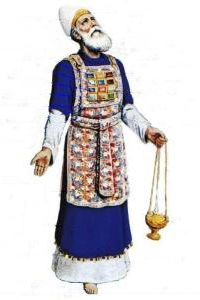
\includegraphics[width=50mm,scale=1.5]{Extras/Melchisedec.jpg}
\vspace{0.4in}  % Create a title for the document and write it in bold font
\LARGE{\textbf{\date}} % Again, do a line break
\linebreak 
% Create a subtitle \large{with Outlines, Statistics, Cross References, and Notes}
\vspace{0.5in}
\begin{flushleft}
\LARGE{Day \#46: Tuesday, 15 February 2022  \\}\vspace{0.25in}
\LARGE{Numbers 16-18 Psalm 46 Proverb 15}
\end{flushleft}
\vspace{0.6in}
\bigskip

\normalsize{Xenia, Oh.\\}
\normalsize{created: \today}
\vspace{1.3in}

\end{flushright}
\end{titlepage}

\newpage 
\tableofcontents\hypertarget{TOC}{}
\listoffigures
\listoftables

\hyphenation{A-bim-e-lech bre-thren E-phra-im  Gib-e-o-nites Jer-u-sa-lem through-out Phil-i-stines The-o-phil-us Am-a-le-kites ven-geance Mesh-el-e-mi-ah onan-ism Phar-a-oh thoughts grev-ous-ness Hach-a-liah adul-ter-er Shad-rach}

%%%%%%%%%%%%%%%%% EXTRA COLORS
%%%%%%%%%%%%%%%%% EXTRA COLORS
%%%%%%%%%%%%%%%%% EXTRA COLORS
\definecolor{champagne}{rgb}{0.97,0.91,0.81}
\definecolor{bone}{rgb}{0.89,0.85,0.79}

\definecolor{ForestGreen}{rgb}{0.00,0.29,0.098}
\definecolor{GIVING}{cmyk}{1,0.0,0.72,.1}

\definecolor{MLPE}{cmyk}{1,1,0,.45}
\definecolor{SOCCER}{cmyk}{.77, 0, .42, .49}
\definecolor{PAYBILL}{cmyk}{0,0.83,0.76,0.07}
\definecolor{SERMON}{cmyk}{.14,.9,0,.30} % aka seance \href{http://www.flatuicolorpicker.com/purple-cmyk-color-model/}{seance}
\definecolor{BIBLE}{cmyk}{0,.17,.74,.17}
\definecolor{WORKBLUE}{cmyk}{1, .5, 0, .6}
\definecolor{myOrange}{cmyk}{0, .4, .98, .03}
\definecolor{myTan}{cmyk}{0.0,.07,.17,.10}
\definecolor{myRed}{cmyk}{0,1,1,0}
\definecolor{myWhite}{cmyk}{0,0,0,0}
\definecolor{BLUESoD}{cmyk}{.97,.84,0,.04}
\definecolor{WHITE}{cmyk}{0,0,0,0}
\definecolor{OLDGOLD}{cmyk}{0.05,0.3,1.00,0}
\definecolor{CASTLETON}{cmyk}{1,0,0.31,0.66}
\definecolor{cadmiumgreen}{rgb}{0.0, 0.42, 0.24}
\definecolor{jungle}{rgb}{0.203,0.4882,0.1718}
\definecolor{MYGOLD}{rgb}{1,.84,0}

\definecolor{MYLIGHTGRAY}{rgb}{.85,.85,.85}

\definecolor{codegreen}{rgb}{0,0.6,0}
\definecolor{codegray}{rgb}{0.5,0.5,0.5}
\definecolor{codepurple}{rgb}{0.58,0,0.82}
\definecolor{backcolour}{rgb}{0.95,0.95,0.92}


\mdfdefinestyle{MyFrame}{%
    linecolor=blue,
    outerlinewidth=2pt,
    roundcorner=5pt,
    innertopmargin=\baselineskip,
    innerbottommargin=\baselineskip,
    innerrightmargin=10pt,
    innerleftmargin=10pt,
    backgroundcolor=gray!25!white}


\mdfdefinestyle{MyFrame2}{%
    linecolor=black,
    outerlinewidth=2pt,
    roundcorner=5pt,
    innertopmargin=\baselineskip,
    innerbottommargin=\baselineskip,
    innerrightmargin=10pt,
    innerleftmargin=10pt,
    backgroundcolor=yellow!25!white}


%%%%%
%% for PFTTIS list
%%%%%

%%% And Joseph said unto
\index[PFTTIS]{And Joseph said unto!Genesis!Gen 40:008}
\index[PFTTIS]{And Joseph said unto!Genesis!Gen 40:012}
\index[PFTTIS]{And Joseph said unto!Genesis!Gen 41:025}
\index[PFTTIS]{And Joseph said unto!Genesis!Gen 42:014}
\index[PFTTIS]{And Joseph said unto!Genesis!Gen 42:018}
\index[PFTTIS]{And Joseph said unto!Genesis!Gen 44:015}
\index[PFTTIS]{And Joseph said unto!Genesis!Gen 45:003}
\index[PFTTIS]{And Joseph said unto!Genesis!Gen 45:004}
\index[PFTTIS]{And Joseph said unto!Genesis!Gen 46:031}
\index[PFTTIS]{And Joseph said unto!Genesis!Gen 48:009}
\index[PFTTIS]{And Joseph said unto!Genesis!Gen 48:018}
\index[PFTTIS]{And Joseph said unto!Genesis!Gen 50:019}
\index[PFTTIS]{And Joseph said unto!Genesis!Gen 50:024}


%%% a shadow
\index[PFTTIS]{a shadow!1Chronicles!1Chr 029:15}
\index[PFTTIS]{a shadow!Job!Job 008:09}
\index[PFTTIS]{a shadow!Job!Job 014:02}
\index[PFTTIS]{a shadow!Job!Job 017:07}
\index[PFTTIS]{a shadow!Psalm!Psa 102:011}
\index[PFTTIS]{a shadow!Psalm!Psa 144:004}
\index[PFTTIS]{a shadow!Ecclesiastes!Eccl 006:012}
\index[PFTTIS]{a shadow!Ecclesiastes!Eccl 008:013}
\index[PFTTIS]{a shadow!Isaiah!Isa 04:006}
\index[PFTTIS]{a shadow!Isaiah!Isa 25:004}
\index[PFTTIS]{a shadow!Jonah!Jnh 04:06}
\index[PFTTIS]{a shadow!Colossians!Col 02:017}
\index[PFTTIS]{a shadow!Hebews!Heb 10:001}

%%% blessed is the man
\index[PFTTIS]{blessed is the man!Psalm!Psa 001:001}
\index[PFTTIS]{blessed is the man!Psalm!Psa 032:002}
\index[PFTTIS]{blessed is the man!Psalm!Psa 034:008}
\index[PFTTIS]{blessed is the man!Psalm!Psa 065:004}
\index[PFTTIS]{blessed is the man!Psalm!Psa 084:005}
\index[PFTTIS]{blessed is the man!Psalm!Psa 084:012}
\index[PFTTIS]{blessed is the man!Psalm!Psa 094:012}
\index[PFTTIS]{blessed is the man!Psalm!Psa 112:001}
\index[PFTTIS]{blessed is the man!Proverbs!Pro 008:034}
\index[PFTTIS]{blessed is the man!Isaiah!Isa 056:002}
\index[PFTTIS]{blessed is the man!Jeremiah!Jer 017:007}
\index[PFTTIS]{blessed is the man!Romans!Rom 004:008}
\index[PFTTIS]{blessed is the man!James!Jam 001:012}


%%% carry them
\index[PFTTIS]{carry them!Leviticus!Lev 14:045}
\index[PFTTIS]{carry them!Numbers!Num 11:012}
\index[PFTTIS]{carry them!Joshua!Jsh 04:003}
\index[PFTTIS]{carry them!1Samuel!1Sam 20:040}
\index[PFTTIS]{carry them!1Kings!1Kng 08:046}
\index[PFTTIS]{carry them!2Chronicles!2Chr 06:036}
\index[PFTTIS]{carry them!Ezra!Ezra 05:015}
\index[PFTTIS]{carry them!Isaiah!Isa 40:011}
\index[PFTTIS]{carry them!Isaiah!Isa 41:016}
\index[PFTTIS]{carry them!Isaiah!Isa 57:013}
\index[PFTTIS]{carry them!Jeremiah!Jer 20:004}
\index[PFTTIS]{carry them!Jeremiah!Jer 20:005}
\index[PFTTIS]{carry them!Jeremiah!Jer 43:012}


\index[PFTTIS]{good tidings!2Samuel!2Sam 18:027}
\index[PFTTIS]{good tidings!1Kings!1Ki 01:042}
\index[PFTTIS]{good tidings!2Kings!2Ki 07:009 (2x)}
\index[PFTTIS]{good tidings!Isaiah!Isa 40:009 (2x)}
\index[PFTTIS]{good tidings!Isaiah!Isa 41:007}
\index[PFTTIS]{good tidings!Isaiah!Isa 52:007}
\index[PFTTIS]{good tidings!Isaiah!Isa 61:001}
\index[PFTTIS]{good tidings!Nahum!Nah 01:005}
\index[PFTTIS]{good tidings!Luke!Lk 02:010}
\index[PFTTIS]{good tidings!1Thessalonians!1Thess 03:006}


%%% dead body
\index[PFTTIS]{dead body!Leviticus!Lev 21:011}
\index[PFTTIS]{dead body!Numbers!Num 06:006}
\index[PFTTIS]{dead body!Numbers!Num 09:006}
\index[PFTTIS]{dead body!Numbers!Num 09:007}
\index[PFTTIS]{dead body!Numbers!Num 09:010}
\index[PFTTIS]{dead body!Numbers!Num 09:011}
\index[PFTTIS]{dead body!Numbers!Num 09:013}
\index[PFTTIS]{dead body!Numbers!Num 09:016}
\index[PFTTIS]{dead body!2Kings!2Ki 08:005}
\index[PFTTIS]{dead body!Isaiah!Isa 26:019}
\index[PFTTIS]{dead body!Jeremiah!Jer 26:023}
\index[PFTTIS]{dead body!Jeremiah!Jer 36:030}
\index[PFTTIS]{dead body!Haggai!Hag 02:013}

%%% great sea
\index[PFTTIS]{great sea!Numbers!Num 34:006}
\index[PFTTIS]{great sea!Numbers!Num 34:007}
\index[PFTTIS]{great sea!Joshua!Jos 01:004}
\index[PFTTIS]{great sea!Joshua!Jos 09:001}
\index[PFTTIS]{great sea!Joshua!Jos 15:012}
\index[PFTTIS]{great sea!Joshua!Jos 15:047}
\index[PFTTIS]{great sea!Joshua!Jos 23:004}
\index[PFTTIS]{great sea!Ezekiel!Eze 47:010}
\index[PFTTIS]{great sea!Ezekiel!Eze 47:015}
\index[PFTTIS]{great sea!Ezekiel!Eze 47:019}
\index[PFTTIS]{great sea!Ezekiel!Eze 47:020}
\index[PFTTIS]{great sea!Ezekiel!Eze 48:028}
\index[PFTTIS]{great sea!Daniel!Dan 07:002}


%%% have forsaken me
\index[PFTTIS]{have forsaken me!Judges!Jdg 10:013}
\index[PFTTIS]{have forsaken me!1Samuel!1Sam 08:008}
\index[PFTTIS]{have forsaken me!1Kings!1Ki 11:033}
\index[PFTTIS]{have forsaken me!2Kings!2Ki 22:017}
\index[PFTTIS]{have forsaken me!2Chronicles!2Chr 12:005}
\index[PFTTIS]{have forsaken me!2Chronicles!2Chr 34:025}
\index[PFTTIS]{have forsaken me!Jeremiah!Jer 01:016}
\index[PFTTIS]{have forsaken me!Jeremiah!Jer 02:013}
\index[PFTTIS]{have forsaken me!Jeremiah!Jer 05:007}
\index[PFTTIS]{have forsaken me!Jeremiah!Jer 05:019}
\index[PFTTIS]{have forsaken me!Jeremiah!Jer 16:011 (2x)}
\index[PFTTIS]{have forsaken me!Jeremiah!Jer 19:004}

%%% no king
\index[PFTTIS]{no king!Judges!Jdg 17:06}
\index[PFTTIS]{no king!Judges!Jdg 18:01}
\index[PFTTIS]{no king!Judges!Jdg 19:01}
\index[PFTTIS]{no king!Judges!Jdg 21:25}
\index[PFTTIS]{no king!1Kings!1Ki 22:47}
\index[PFTTIS]{no king!2Kings!2Ki 23:25}
\index[PFTTIS]{no king!Nehemiah!Neh 13:26}
\index[PFTTIS]{no king!Psalms!Psa 033:016}
\index[PFTTIS]{no king!Proverbs!Pro 30:27}
\index[PFTTIS]{no king!Daniel!Dan 02:10}
\index[PFTTIS]{no king!Hosea!Hos 10:03}
\index[PFTTIS]{no king!Micah!Mic 04:09}
\index[PFTTIS]{no king!John!Jhn 19:15}


%%% rebellious house
\index[PFTTIS]{rebellious house!Exodus!Exo 02:005}
\index[PFTTIS]{rebellious house!Exodus!Exo 02:006}
\index[PFTTIS]{rebellious house!Exodus!Exo 02:008}
\index[PFTTIS]{rebellious house!Exodus!Exo 03:009}
\index[PFTTIS]{rebellious house!Exodus!Exo 03:026}
\index[PFTTIS]{rebellious house!Exodus!Exo 03:027}
\index[PFTTIS]{rebellious house!Exodus!Exo 12:002 (2x)}
\index[PFTTIS]{rebellious house!Exodus!Exo 12:003}
\index[PFTTIS]{rebellious house!Exodus!Exo 12:009}
\index[PFTTIS]{rebellious house!Exodus!Exo 12:025}
\index[PFTTIS]{rebellious house!Exodus!Exo 17:012}
\index[PFTTIS]{rebellious house!Exodus!Exo 24:003}

%%% seek him
\index[PFTTIS]{seek him!Deuteronomy!Deu 04:029}\index[PFTTIS]{seek him!1Samuel!1Sam 23:025}
\index[PFTTIS]{seek him!1Chronicles!1Chr 28:009}
\index[PFTTIS]{seek him!2Chronicles!1Chr 15:002}
\index[PFTTIS]{seek him!Ezra!Ezr 08:022}
\index[PFTTIS]{seek him!Psalms!Psa 022:026}
\index[PFTTIS]{seek him!Psalms!Psa 024:006}
\index[PFTTIS]{seek him!Psalms!Psa 119:002}
\index[PFTTIS]{seek him!SoS!SoS 03:002}
\index[PFTTIS]{seek him!SoS!SoS 06:001}
\index[PFTTIS]{seek him!Hosea!Hos 07:010}
\index[PFTTIS]{seek him!Amos!Amo 05:008}
\index[PFTTIS]{seek him!Hebrews!Heb 11:0063}


%%% seek ye
\index[PFTTIS]{seek ye!Isaiah!Isa 34:016}
\index[PFTTIS]{seek ye!Isaiah!Isa 45:019}
\index[PFTTIS]{seek ye!Isaiah!Isa 55:006}
\index[PFTTIS]{seek ye!Amos!Amos 5:004}
\index[PFTTIS]{seek ye!John!John 1:38}
\index[PFTTIS]{seek ye!John!John 18:4}
\index[PFTTIS]{seek ye!John!John 18:7}
\index[PFTTIS]{seek ye!Matthew!Matt 6:33}
\index[PFTTIS]{seek ye!Numbers!Num 16:10}
\index[PFTTIS]{seek ye!Luke!Luke 12:31}
\index[PFTTIS]{seek ye!Luke!Luke 24:5}
\index[PFTTIS]{seek ye!Psalm!Psa 27:8}
\index[PFTTIS]{seek ye!Zephaniah!Zeph 2:3}

%%% the uncircumcised
\index[PFTTIS]{the uncircumcised!Genesis!Gen 17:014}
\index[PFTTIS]{the uncircumcised!Judges!Jdg 14:003}
\index[PFTTIS]{the uncircumcised!Judges!Jdg 15:018}
\index[PFTTIS]{the uncircumcised!2Samuel!2Sam 01:020}
\index[PFTTIS]{the uncircumcised!Isaiah!Isa 02:001}
\index[PFTTIS]{the uncircumcised!Jeremiah!Jer 09:025}
\index[PFTTIS]{the uncircumcised!Ezekiel!Eze 28:010}
\index[PFTTIS]{the uncircumcised!Ezekiel!Eze 31:018}
\index[PFTTIS]{the uncircumcised!Ezekiel!Eze 32:019}
\index[PFTTIS]{the uncircumcised!Ezekiel!Eze 32:027}
\index[PFTTIS]{the uncircumcised!Ezekiel!Eze 32:028}
\index[PFTTIS]{the uncircumcised!Ezekiel!Eze 32:029}
\index[PFTTIS]{the uncircumcised!Ezekiel!Eze 32:032}

%%% worship him
\index[PFTTIS]{worship him!Psalms!Psa 97:007}
\index[PFTTIS]{worship him!Zephaniah!Zeph 02:011}
\index[PFTTIS]{worship him!Matthew!Matt 02:002}
\index[PFTTIS]{worship him!Matthew!Matt 02:008}
\index[PFTTIS]{worship him!John!John 04:023}
\index[PFTTIS]{worship him!John!John 04:024 (2x)} 
\index[PFTTIS]{worship him!Acts!Acts 17:023}
\index[PFTTIS]{worship him!Hebrews!Heb 01:006}
\index[PFTTIS]{worship him!Revelation!Rev 04:010}
\index[PFTTIS]{worship him!Revelation!Rev 13:008}
\index[PFTTIS]{worship him!Revelation!Rev 14:007}
\index[PFTTIS]{worship him!Revelation!Rev 19:010}


%%%%%
%% for PFTTIS list
%%%%%

%%% afflictions
\index[WFTTIS]{afflictions!Psalms!Psa 34:019}
\index[WFTTIS]{afflictions!Psalms!Psa 132:001}
\index[WFTTIS]{afflictions!Acts!Acts 07:010}
\index[WFTTIS]{afflictions!Acts!Acts 20:023}
\index[WFTTIS]{afflictions!2Corinthians!2Cor 06:004}
\index[WFTTIS]{afflictions!Colossians!Col 01:024}
\index[WFTTIS]{afflictions!1Thessalonians!1Thess 03:003}
\index[WFTTIS]{afflictions!2Timothy!2Tim 01:008}
\index[WFTTIS]{afflictions!2Timothy!2Tim 03:011}
\index[WFTTIS]{afflictions!2Timothy!2Tim 04:005}
\index[WFTTIS]{afflictions!Hebrews!Heb 10:032}
\index[WFTTIS]{afflictions!Hebrews!Heb 10:033}
\index[WFTTIS]{afflictions!1Peter!1Pet 05:009}

%%% acsend
\index[WFTTIS]{acsend!Joshua!Jos 06:05}
\index[WFTTIS]{acsend!Psalm!Psa 024:003}
\index[WFTTIS]{acsend!Psalm!Psa 135:007}
\index[WFTTIS]{acsend!Psalm!Psa 139:008}
\index[WFTTIS]{acsend!Isaiah!Isa 14:013}
\index[WFTTIS]{acsend!Isaiah!Isa 14:014}
\index[WFTTIS]{acsend!Jeremiah!Jer 10:013}
\index[WFTTIS]{acsend!Jeremiah!Jer 51:016}
\index[WFTTIS]{acsend!Ezekiel!Eze 38:009}
\index[WFTTIS]{acsend!John!John 06:062}
\index[WFTTIS]{acsend!John!John 20:017}
\index[WFTTIS]{acsend!Romans!Rom 10:006}
\index[WFTTIS]{acsend!Revelation!Rev 17:008}

%%% Assyrian
\index[WFTTIS]{Assyrian!Isaiah!Isa 10:005}
\index[WFTTIS]{Assyrian!Isaiah!Isa 10:024}
\index[WFTTIS]{Assyrian!Isaiah!Isa 14:025}
\index[WFTTIS]{Assyrian!Isaiah!Isa 19:023}
\index[WFTTIS]{Assyrian!Isaiah!Isa 23:013}
\index[WFTTIS]{Assyrian!Isaiah!Isa 30:031}
\index[WFTTIS]{Assyrian!Isaiah!Isa 31:008}
\index[WFTTIS]{Assyrian!Isaiah!Isa 52:004}
\index[WFTTIS]{Assyrian!Ezekiel!Eze 31:003}
\index[WFTTIS]{Assyrian!Hosea!Hos 05:013}
\index[WFTTIS]{Assyrian!Hosea!Hos 11:005}
\index[WFTTIS]{Assyrian!Micah!Hos 05:005}
\index[WFTTIS]{Assyrian!Micah!Hos 05:006}

%%% blot
\index[WFTTIS]{blot!Exodus!Exo 32:032}
\index[WFTTIS]{blot!Exodus!Exo 32:033}
\index[WFTTIS]{blot!Numbers!Num 05:026}
\index[WFTTIS]{blot!Deuteronomy!Deut 09:014}
\index[WFTTIS]{blot!Deuteronomy!Deut 25:019}
\index[WFTTIS]{blot!Deuteronomy!Deut 29:020}
\index[WFTTIS]{blot!2Kings!2Ki 14:027}
\index[WFTTIS]{blot!Job!Job 31:007}
\index[WFTTIS]{blot!Psalms!Psa 51:001}
\index[WFTTIS]{blot!Psalms!Psa 51:009}
\index[WFTTIS]{blot!Proverbs!Pro 09:007}
\index[WFTTIS]{blot!Jeremiah!Jer 18:023}
\index[WFTTIS]{blot!Revelation!Rev 03:005}


%%% chain
\index[WFTTIS]{chain!Genesis!Gen 41:042}
\index[WFTTIS]{chain!1Kings!1Ki 07:017}
\index[WFTTIS]{chain!Psalms!Psa 73:006}
\index[WFTTIS]{chain!SoS!Sos 04:009}
\index[WFTTIS]{chain!Lamentations!Lam 03:007}
\index[WFTTIS]{chain!Ezekiel!Eze 07:023}
\index[WFTTIS]{chain!Ezekiel!Eze 16:011}
\index[WFTTIS]{chain!Daniel!Dan 05:007}
\index[WFTTIS]{chain!Daniel!Dan 05:016}
\index[WFTTIS]{chain!Daniel!Dan 05:029}
\index[WFTTIS]{chain!Acts!Acts 28:020}
\index[WFTTIS]{chain!2Timothy!2Tim 01:016}
\index[WFTTIS]{chain!Revelation!Rev 20:001}


%%% controversy
\index[WFTTIS]{controversy!Deuteronomy!Deu 17:008}
\index[WFTTIS]{controversy!Deuteronomy!Deu 19:017}
\index[WFTTIS]{controversy!Deuteronomy!Deu 21:005}
\index[WFTTIS]{controversy!Deuteronomy!Deu 25:001}
\index[WFTTIS]{controversy!2Samuel!2Sam 15:002}
\index[WFTTIS]{controversy!Isaiah!Isa 34:008}
\index[WFTTIS]{controversy!Jeremiah!Jer 25:031}
\index[WFTTIS]{controversy!Ezekiel!Eze 44:024}
\index[WFTTIS]{controversy!Hosea!Hos 04:001}
\index[WFTTIS]{controversy!Hosea!Hos 12:002}
\index[WFTTIS]{controversy!Micah!Mic 06:002 (2x)}
\index[WFTTIS]{controversy!1Timothy!1Tim 03:016}


%%% Dagon/Dagon's
\index[WFTTIS]{Dagon!Judges!Jdg 16:023}
\index[WFTTIS]{Dagon!1Samuel!1Sam 05:002 (2x)}
\index[WFTTIS]{Dagon!1Samuel!1Sam 05:003 (2x)}
\index[WFTTIS]{Dagon!1Samuel!1Sam 05:004 (3x)}
\index[WFTTIS]{Dagon!1Samuel!1Sam 05:005 (3x)}
\index[WFTTIS]{Dagon!1Samuel!1Sam 05:007}
\index[WFTTIS]{Dagon!1Chronicles!1Chr 10:010}

%%% disobedient
\index[WFTTIS]{disobedient!1Kings!1Ki 13:026}
\index[WFTTIS]{disobedient!Nehemiah!Neh 09:026}
\index[WFTTIS]{disobedient!Luke!Luke 01:017}
\index[WFTTIS]{disobedient!Acts!Acts 26:019}
\index[WFTTIS]{disobedient!Romans!Rom 01:030}
\index[WFTTIS]{disobedient!Romans!Rom 10:021}
\index[WFTTIS]{disobedient!1Timothy!1Tim 01:009}
\index[WFTTIS]{disobedient!2Timothy!2Tim 03:002}
\index[WFTTIS]{disobedient!Titus!Titus 01:016}
\index[WFTTIS]{disobedient!Titus!Titus 03:003}
\index[WFTTIS]{disobedient!1Peter!1Pet 02:007}
\index[WFTTIS]{disobedient!1Peter!1Pet 02:008}
\index[WFTTIS]{disobedient!1Peter!1Pet 03:020}


%%% doubt
\index[WFTTIS]{doubt!Genesis!Gen 37:033}
\index[WFTTIS]{doubt!Deuteronomy!Deu 28:066}
\index[WFTTIS]{doubt!Job!Job 12:002}
\index[WFTTIS]{doubt!Matthew!Matt 14:031}
\index[WFTTIS]{doubt!Matthew!Matt 21:021}
\index[WFTTIS]{doubt!Mark!Mk 11:023}
\index[WFTTIS]{doubt!Luke!Lk 11:020}
\index[WFTTIS]{doubt!John!Jhn 10:024}
\index[WFTTIS]{doubt!Acts!Acts 02:012}
\index[WFTTIS]{doubt!Acts!Acts 28:004}
\index[WFTTIS]{doubt!1Corinthians!1Cor 09:010}
\index[WFTTIS]{doubt!Galatians!Gal 04:020}
\index[WFTTIS]{doubt!1John!1Jhn 02:019}


%%% dungeon
\index[WFTTIS]{dungeon!Genesis!Gen 40:015}
\index[WFTTIS]{dungeon!Genesis!Gen 41:014}
\index[WFTTIS]{dungeon!Exodus!Exo 12:029}
\index[WFTTIS]{dungeon!Jeremiah!Jer 37:016}
\index[WFTTIS]{dungeon!Jeremiah!Jer 38:006 (2x)}
\index[WFTTIS]{dungeon!Jeremiah!Jer 38:007}
\index[WFTTIS]{dungeon!Jeremiah!Jer 38:009}
\index[WFTTIS]{dungeon!Jeremiah!Jer 38:010}
\index[WFTTIS]{dungeon!Jeremiah!Jer 38:011}
\index[WFTTIS]{dungeon!Jeremiah!Jer 38:013}
\index[WFTTIS]{dungeon!Lamentations!Lam 03:053}
\index[WFTTIS]{dungeon!Lamentations!Lam 03:055}


%%% error
\index[WFTTIS]{error!2Samuel!2Sam 06:007}
\index[WFTTIS]{error!Job!Job 19:004}
\index[WFTTIS]{error!Ecclesiastes!Ecc 05:006}
\index[WFTTIS]{error!Ecclesiastes!Ecc 10:005}
\index[WFTTIS]{error!Isaiah!Isa 32:006}
\index[WFTTIS]{error!Daniel!Dan 06:004}
\index[WFTTIS]{error!Matthew!Matt 27:064}
\index[WFTTIS]{error!Romans!Rom 01:027}
\index[WFTTIS]{error!James!Jam 05:020}
\index[WFTTIS]{error!2Peter!2Pet 02:018}
\index[WFTTIS]{error!2Peter!2Pet 03:017}
\index[WFTTIS]{error!1John!1Jn 04:006}
\index[WFTTIS]{error!Jude!Jude 01:011}

%%% fourish
\index[WFTTIS]{fourish!Psalms!Psa 072:007}
\index[WFTTIS]{fourish!Psalms!Psa 072:016}
\index[WFTTIS]{fourish!Psalms!Psa 092:007}
\index[WFTTIS]{fourish!Psalms!Psa 092:012}
\index[WFTTIS]{fourish!Psalms!Psa 092:013}
\index[WFTTIS]{fourish!Psalms!Psa 132:018}
\index[WFTTIS]{fourish!Proverbs!Pro 11:28}
\index[WFTTIS]{fourish!Proverbs!Pro 14:11}
\index[WFTTIS]{fourish!Ecclesiastes!Ecc 12:05}
\index[WFTTIS]{fourish!SongOfSolomon!SOS 07:12}
\index[WFTTIS]{fourish!Isaiah!Isa 17:11}
\index[WFTTIS]{fourish!Isaiah!Isa 66:14}
\index[WFTTIS]{fourish!Ezekiel!Eze 17:24}




%%% giants
\index[WFTTIS]{giants!Genesis!Gen 06:004}
\index[WFTTIS]{giants!Numbers!Num 13:033}
\index[WFTTIS]{giants!Deuteronomy!Deut 02:011}
\index[WFTTIS]{giants!Deuteronomy!Deut 02:021}
\index[WFTTIS]{giants!Deuteronomy!Deut 03:011}
\index[WFTTIS]{giants!Deuteronomy!Deut 03:013}
\index[WFTTIS]{giants!Joshua!Josh 12:004}
\index[WFTTIS]{giants!Joshua!Josh 13:012}
\index[WFTTIS]{giants!Joshua!Josh 15:008}
\index[WFTTIS]{giants!Joshua!Josh 17:015}
\index[WFTTIS]{giants!Joshua!Josh 16:016}

%%% good man
\index[WFTTIS]{good man!2 Samuel!2Sa 18:27}
%(1) Psalms 37:23 [5]
%(1) Psalms 112:5 [2]
%(1) Proverbs 12:2 [2]
%(1) Proverbs 13:22 [2]
%(1) Proverbs 14:14 [14]
%(1) Micah 7:2 [2]
%(1) Matthew 12:35 [2]
%(1) Luke 6:45 [2]
%(1) Luke 23:50 [15]
%(1) John 7:12 [17]
%(1) Acts 11:24 [5]
%(1) Romans 5:7 [14]

%%% Hinnom
\index[WFTTIS]{Hinnom!Joshua!Jsh 15:008}
\index[WFTTIS]{Hinnom!Joshua!Jsh 18:016}
\index[WFTTIS]{Hinnom!2Kings!2Ki 23:010}
\index[WFTTIS]{Hinnom!2Chronicles!2Chr 28:003}
\index[WFTTIS]{Hinnom!2Chronicles!2Chr 33:006}
\index[WFTTIS]{Hinnom!Nehemiah!Neh 11:030}
\index[WFTTIS]{Hinnom!Jeremiah!Jer 07:031}
\index[WFTTIS]{Hinnom!Jeremiah!Jer 07:032}
\index[WFTTIS]{Hinnom!Jeremiah!Jer 19:002}
\index[WFTTIS]{Hinnom!Jeremiah!Jer 19:006}
\index[WFTTIS]{Hinnom!Jeremiah!Jer 32:035}

%%% inclined
\index[WFTTIS]{inclined!Judges!Jdg 09:003}
\index[WFTTIS]{inclined!Psalms!Psa 040:001}
\index[WFTTIS]{inclined!Psalms!Psa 116:002}
\index[WFTTIS]{inclined!Psalms!Psa 119:112}
\index[WFTTIS]{inclined!Proverbs!Pro 05:13}
\index[WFTTIS]{inclined!Jeremiah!Jer 07:24}
\index[WFTTIS]{inclined!Jeremiah!Jer 07:26}
\index[WFTTIS]{inclined!Jeremiah!Jer 11:08}
\index[WFTTIS]{inclined!Jeremiah!Jer 17:23}
\index[WFTTIS]{inclined!Jeremiah!Jer 25:04}
\index[WFTTIS]{inclined!Jeremiah!Jer 34:14}
\index[WFTTIS]{inclined!Jeremiah!Jer 35:15}
\index[WFTTIS]{inclined!Jeremiah!Jer 44:05}


%%% laughed
\index[WFTTIS]{laughed!Genesis!Gen 17:017}
\index[WFTTIS]{laughed!Genesis!Gen 18:012}
\index[WFTTIS]{laughed!Genesis!Gen 18:015}
\index[WFTTIS]{laughed!2Kings!2Ki 19:021}
\index[WFTTIS]{laughed!2Chronicles!2Chr 30:010}
\index[WFTTIS]{laughed!Nehemiah!Neh 02:019}
\index[WFTTIS]{laughed!Job!Job 12:004}
\index[WFTTIS]{laughed!Job!Job 29:024}
\index[WFTTIS]{laughed!Isaiah!Isa 37:022}
\index[WFTTIS]{laughed!Ezekiel!Ezek 23:032}
\index[WFTTIS]{laughed!Matthew!Matt 09:024}
\index[WFTTIS]{laughed!Mark!Mk 05:040}
\index[WFTTIS]{laughed!Luke!Lk 08:053}

%%% liar
\index[WFTTIS]{liar!Job!Job 24:025}
\index[WFTTIS]{liar!Proverbs!Pro 17:004}
\index[WFTTIS]{liar!Proverbs!Pro 19:022}
\index[WFTTIS]{liar!Proverbs!Pro 30:006}
\index[WFTTIS]{liar!Jeremiah!Jer 15:018}
\index[WFTTIS]{liar!John!Jhn 08:044}
\index[WFTTIS]{liar!John!Jhn 08:055}
\index[WFTTIS]{liar!Romans!Rom 03:004}
\index[WFTTIS]{liar!1John!1Jhn 01:010}
\index[WFTTIS]{liar!1John!1Jhn 02:004}
\index[WFTTIS]{liar!1John!1Jhn 02:022}
\index[WFTTIS]{liar!1John!1Jhn 04:020}
\index[WFTTIS]{liar!1John!1Jhn 05:010}

%%% palsy
\index[WFTTIS]{palsy!Matthew!Matt 04:024}
\index[WFTTIS]{palsy!Matthew!Matt 08:006}
\index[WFTTIS]{palsy!Matthew!Matt 09:002}
\index[WFTTIS]{palsy!Matthew!Matt 09:006}
\index[WFTTIS]{palsy!Mark!Mk 02:003}
\index[WFTTIS]{palsy!Mark!Mk 02:004}
\index[WFTTIS]{palsy!Mark!Mk 02:005}
\index[WFTTIS]{palsy!Mark!Mk 02:009}
\index[WFTTIS]{palsy!Mark!Mk 02:010}
\index[WFTTIS]{palsy!Luke!Lk 05:018}
\index[WFTTIS]{palsy!Luke!Lk 05:024}
\index[WFTTIS]{palsy!Acts!Acts 09:033}

%%% Profitable
\index[WFTTIS]{profitable!Job!Job 22:002 (2x)}
\index[WFTTIS]{profitable!Ecclesiastes!Ecc 10:010}
\index[WFTTIS]{profitable!Isaiah!Isa 44:010}
\index[WFTTIS]{profitable!Jeremiah!Jer 13:007}
\index[WFTTIS]{profitable!Matthew!Matt 05:029}
\index[WFTTIS]{profitable!Matthew!Matt 05:030}
\index[WFTTIS]{profitable!Acts!Acts 20:020}
\index[WFTTIS]{profitable!1Timothy!1Tim 04:008}
\index[WFTTIS]{profitable!2Timothy!2Tim 03:016}
\index[WFTTIS]{profitable!2Timothy!2Tim 04:011}
\index[WFTTIS]{profitable!Titus!Titus 03:008}
\index[WFTTIS]{profitable!Philemon!Phlm 01:011}

%%% Rechab
\index[WFTTIS]{Rechab!2Samuel!2Sam 04:002}
\index[WFTTIS]{Rechab!2Samuel!2Sam 04:005}
\index[WFTTIS]{Rechab!2Samuel!2Sam 04:006}
\index[WFTTIS]{Rechab!2Samuel!2Sam 04:009}
\index[WFTTIS]{Rechab!2KIngs!2Ki 10:015}
\index[WFTTIS]{Rechab!2KIngs!2Ki 10:023}
\index[WFTTIS]{Rechab!1Chronicles!1Chr 02:055}
\index[WFTTIS]{Rechab!Nehemiah!Neh 03:014}
\index[WFTTIS]{Rechab!Jeremiah!Jer 35:006}
\index[WFTTIS]{Rechab!Jeremiah!Jer 35:008}
\index[WFTTIS]{Rechab!Jeremiah!Jer 35:014}
\index[WFTTIS]{Rechab!Jeremiah!Jer 35:016}
\index[WFTTIS]{Rechab!Jeremiah!Jer 35:019}

%%% serpents
\index[WFTTIS]{serpents!Exodus!Exo 07:012}
\index[WFTTIS]{serpents!Numbers!Num 21:006}
\index[WFTTIS]{serpents!Numbers!Num 21:007}
\index[WFTTIS]{serpents!Deuteronomy!Deu 08:015}
\index[WFTTIS]{serpents!Deuteronomy!Deu 32:024}
\index[WFTTIS]{serpents!Jeremiah!Jer 08:017}
\index[WFTTIS]{serpents!Matthew!Matt 10:016}
\index[WFTTIS]{serpents!Matthew!Matt 23:033}
\index[WFTTIS]{serpents!Mark!Mk 16:018}
\index[WFTTIS]{serpents!Luke!Lk 10:019}
\index[WFTTIS]{serpents!1Corinthians!1Cor 10:009}
\index[WFTTIS]{serpents!James!Jas 03:007}
\index[WFTTIS]{serpents!Revelation!Rev 09:019}

%%% short
\index[WFTTIS]{short!Numbers!Num 11:023}
\index[WFTTIS]{short!2Kings!2Ki 10:032}
\index[WFTTIS]{short!Job!Job 17:012}
\index[WFTTIS]{short!Job!Job 20:005}
\index[WFTTIS]{short!Psalms!Psa 89:047}
\index[WFTTIS]{short!Romans!Rom 03:023}
\index[WFTTIS]{short!Romans!Rom 09:028  (2x)}
\index[WFTTIS]{short!1Corinthians!1Cor 07:029}
\index[WFTTIS]{short!1Thessalonians!1Thess 02:017}
\index[WFTTIS]{short!Hebrews!Heb 04:001}
\index[WFTTIS]{short!Revelation!Rev 12:012}
\index[WFTTIS]{short!Revelation!Rev 17:010}

%%% smiteth
\index[WFTTIS]{smiteth!Exodus!Exo 21:012}
\index[WFTTIS]{smiteth!Exodus!Exo 21:15}
\index[WFTTIS]{smiteth!Deuteronomy!Dt 25:11}
\index[WFTTIS]{smiteth!Deuteronomy!Dt 27:24}
\index[WFTTIS]{smiteth!Joshua!Jsh 15:16}
\index[WFTTIS]{smiteth!Judges!Jdg 15:16}
\index[WFTTIS]{smiteth!2 Samuel!2Sa 05:08}
\index[WFTTIS]{smiteth!1Chronicles!1Chr 11:06}
\index[WFTTIS]{smiteth!Job!1Chr 26:12}
\index[WFTTIS]{smiteth!Isaiah!Isa 09:13}
\index[WFTTIS]{smiteth!Lamentations!Lam 03:30}
\index[WFTTIS]{smiteth!Ezekiel!Eze 07:09}
\index[WFTTIS]{smiteth!Luke!Lk 06:29}



%%% vanities
\index[WFTTIS]{vanities!Deuteronomy!Deut 21:021}
\index[WFTTIS]{vanities!1Kings!1Ki 16:013}
\index[WFTTIS]{vanities!1Kings!1Ki 16:026}
\index[WFTTIS]{vanities!Psalms!Psa 031:006}
\index[WFTTIS]{vanities!Ecclesiastes!Ecc 01:002 (2x)}
\index[WFTTIS]{vanities!Ecclesiastes!Ecc 05:007}
\index[WFTTIS]{vanities!Ecclesiastes!Ecc 12:008}
\index[WFTTIS]{vanities!Jeremiah!Jer 08:019}
\index[WFTTIS]{vanities!Jeremiah!Jer 10:008}
\index[WFTTIS]{vanities!Jeremiah!Jer 14:022}
\index[WFTTIS]{vanities!Jonah!Jnh 02:008}
\index[WFTTIS]{vanities!Acts!Acts 14:015}



%%%%%
%% for PFTTIS list
%%%%%

%%% worm
\index[WFITV]{worm!Exodus!Exo 16:024}
\index[WFITV]{worm!Job!Job 17:014}
\index[WFITV]{worm!Job!Job 24:029}
\index[WFITV]{worm!Job!Job 25:005 (2x)}
\index[WFITV]{worm!Psalms!Psa 022:006}
\index[WFITV]{worm!Isaiah!Isa 14:011}
\index[WFITV]{worm!Isaiah!Isa 41:014}
\index[WFITV]{worm!Isaiah!Isa 51:008}
\index[WFITV]{worm!Isaiah!Isa 66:024}
\index[WFITV]{worm!Jonah!Jnh 04:007}
\index[WFITV]{worm!Mark!Mk 09:044}
\index[WFITV]{worm!Mark!Mk 09:046}
\index[WFITV]{worm!Mark!Mk 09:048}


%\subsubsection{Title}
%\textbf{Introduction:} Isaiah 46 
%\index[speaker]{Speaker!Isaiah 49 (Title}
%\index[series]{Book (Speaker)!IPassage (Title)}
%\index[date]{2017/07/09!Isaiah 49 (Title)}
%\begin{compactenum}[I.]
%    \item  \textbf{Point} \index[scripture]{Isaiah!IPassage} (IPassage)
%\end{compactenum}




  


%\input{02OT-Exodus/ExodusIntroduction}
\newpage
\begin{figure}
\begin{center}
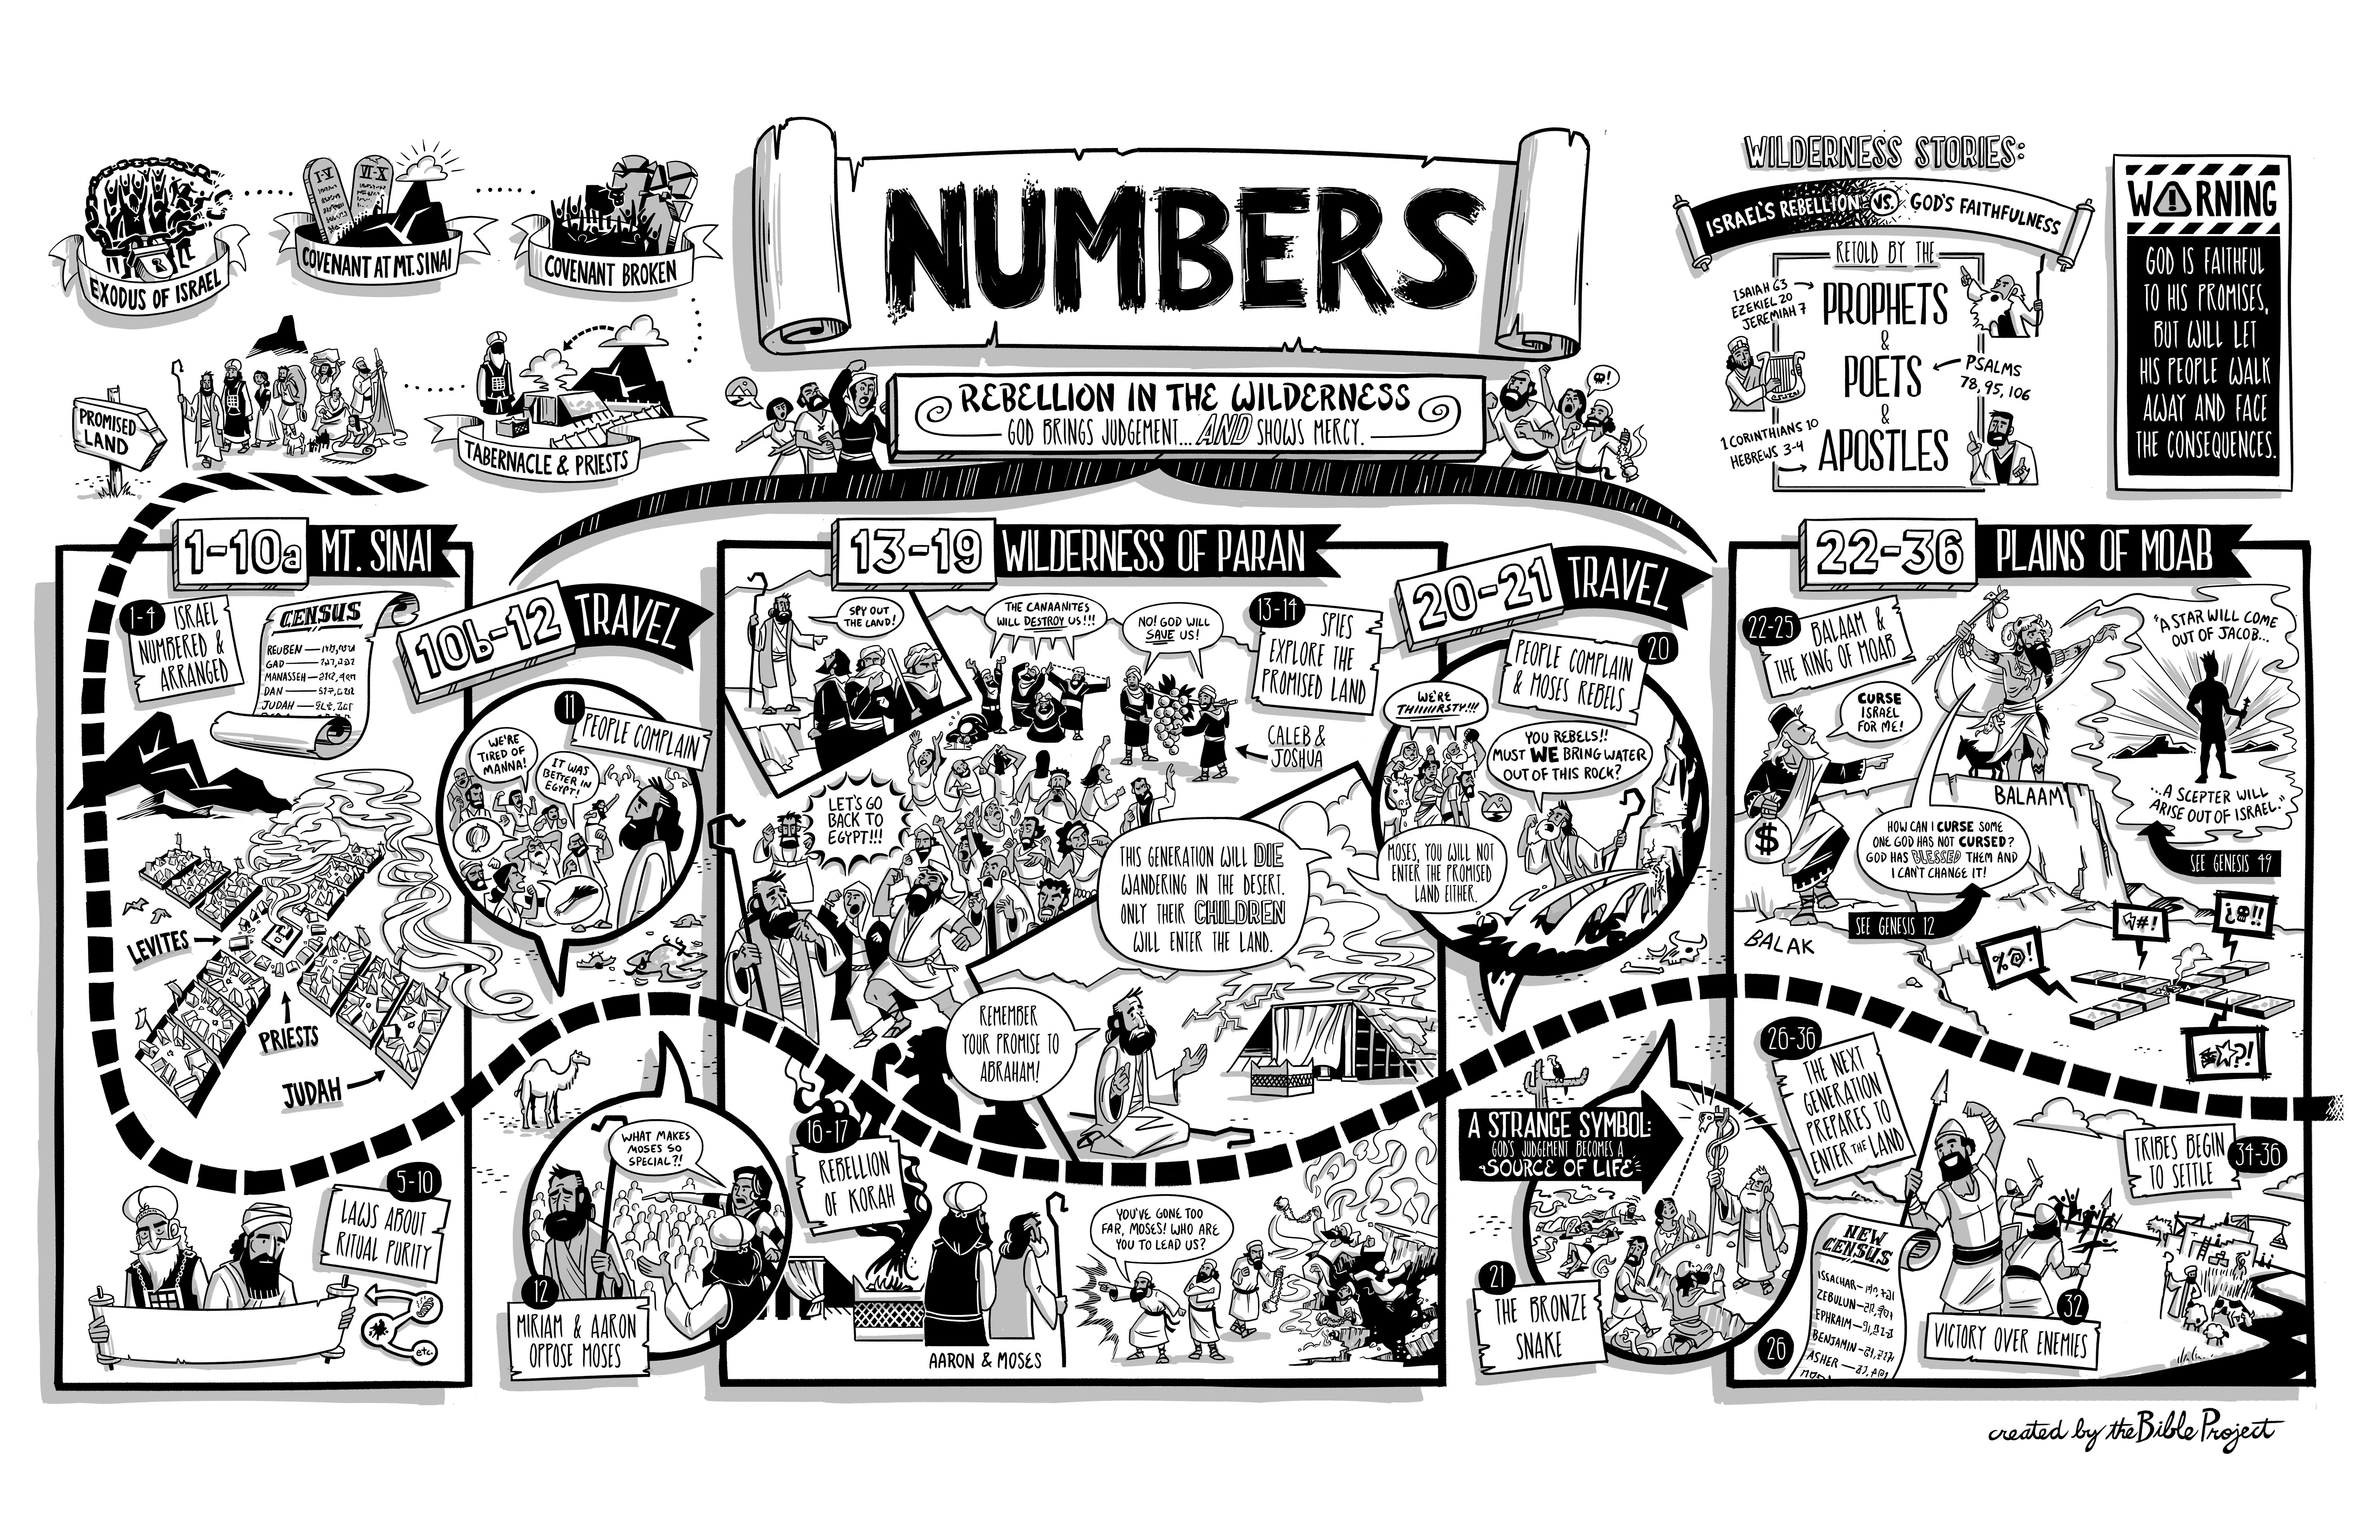
\includegraphics[scale=0.5, angle=90]{04OT-Numbers/References/BibleProject-Numbers.jpg}
\caption[Numbers from the Bible Project]{Numbers from the Bible Project}
\label{fig:Numbers from the Bible Project}
\end{center}
\end{figure}

\newpage
\begin{figure}
\begin{center}
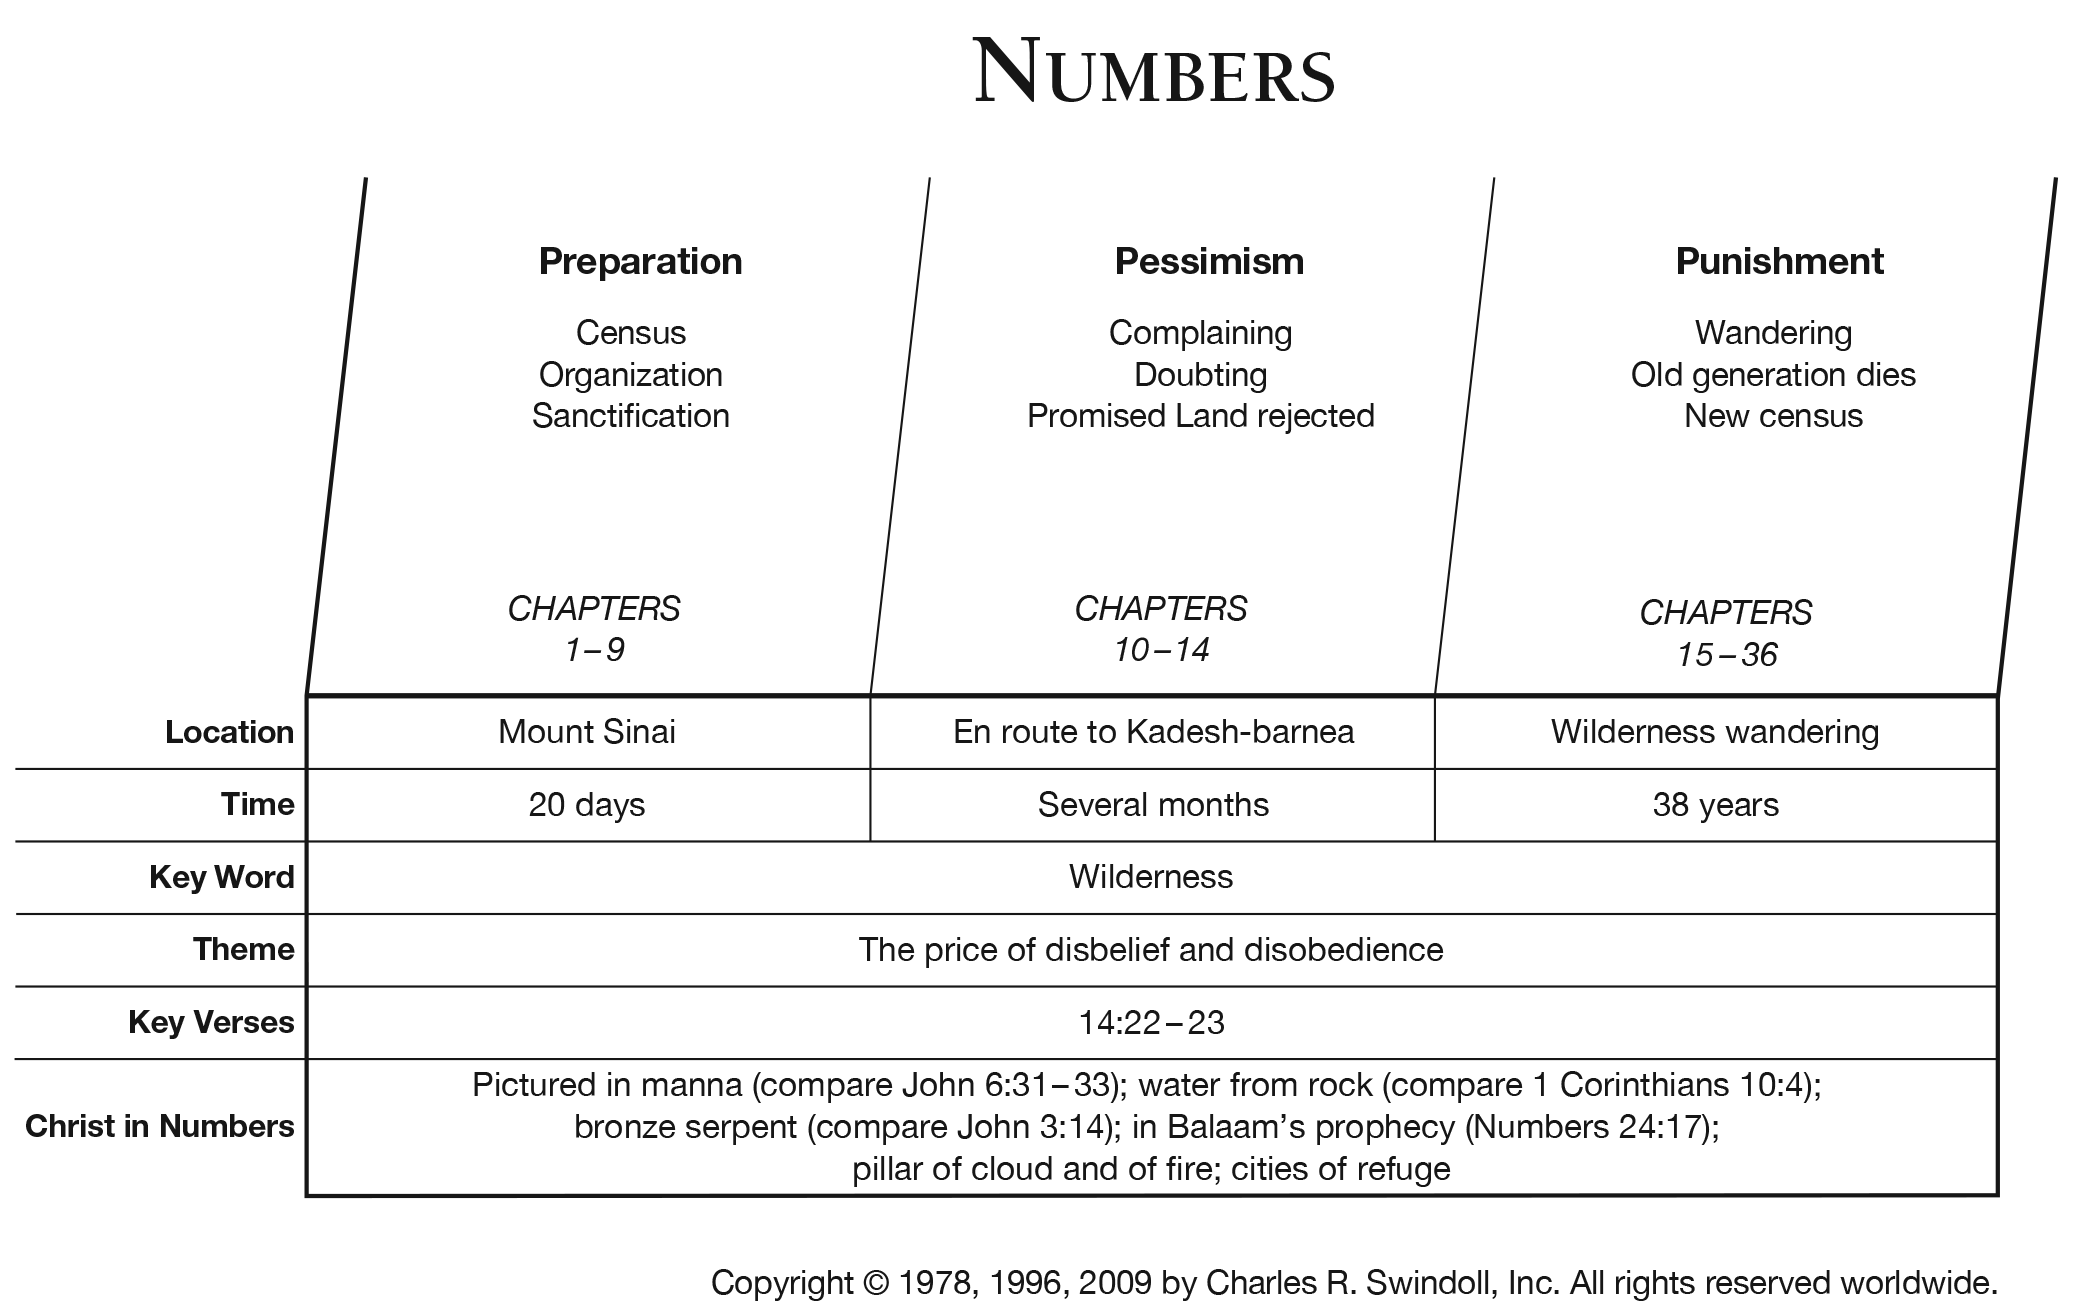
\includegraphics[scale=0.3, angle=90]{04OT-Numbers/References/Swindoll-Numbers.png}
\caption[Numbers by Swindoll]{Numbers by Swindoll}
\label{fig:Numbers by Swindoll}
\end{center}
\end{figure}

\newpage
\begin{figure}
\begin{center}
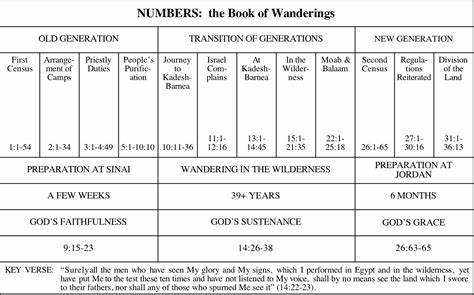
\includegraphics[scale=1.2, angle=90]{04OT-Numbers/References/Numbers.jpg}
\caption[Numbers by Unknown]{Numbers by Unknown}
\label{fig:Numbers by Unknown}
\end{center}
\end{figure}

\newpage
\begin{figure}
\begin{center}
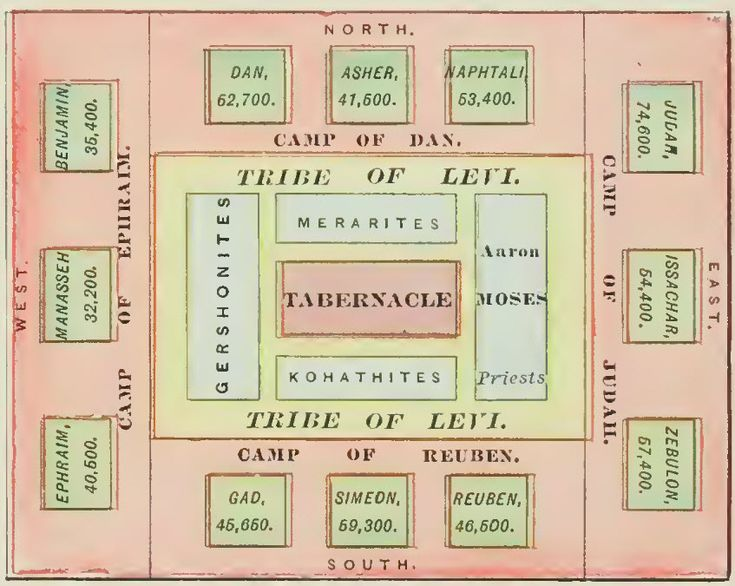
\includegraphics[scale=.8, angle=0]{04OT-Numbers/References/LayoutOfTribesAndTabernacle.jpg}
\caption[Layout of Tribes and Tabernacle]{Layout of Tribes and Tabernacle}
\label{fig:Layout of Tribes and Tabernacle}
\end{center}
\end{figure}


\chapter{Numbers 16}

\begin{figure}
  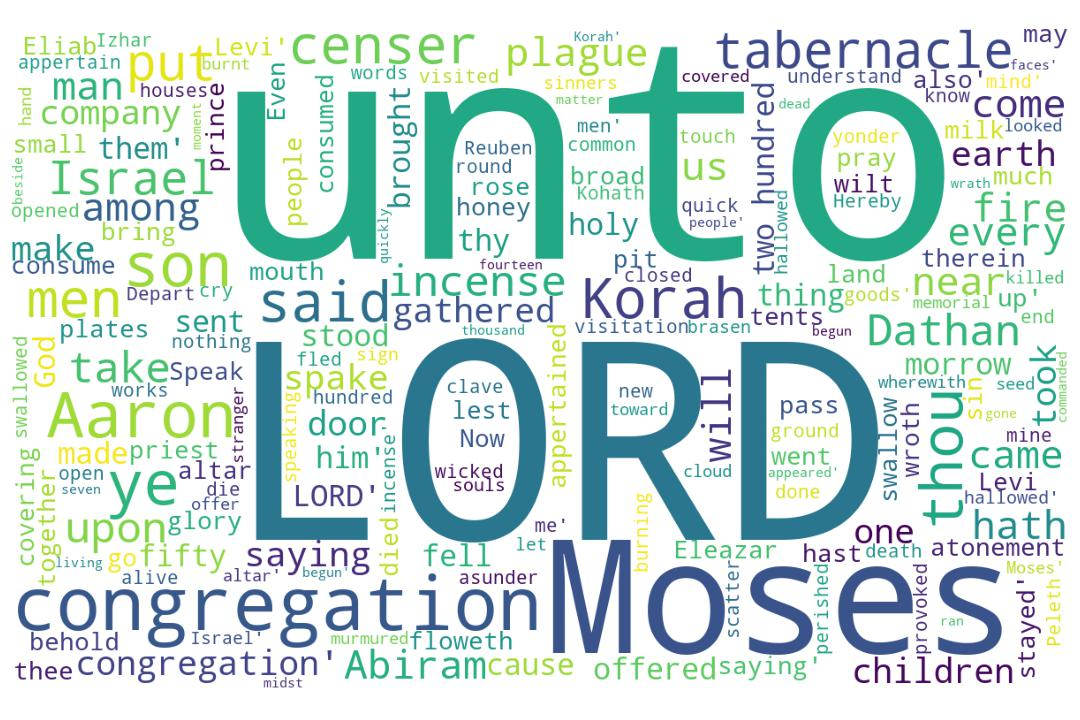
\includegraphics[width=\linewidth]{04OT-Numbers/Numbers16-WordCloud.jpg}
  \caption{Numbers 16 Word Cloud}
  \label{fig:Numbers 16 word Cloud}
\end{figure}

\marginpar{\scriptsize \centering \fcolorbox{bone}{lime}{\textbf{THE KORAH INCIDENT}}\\ (Numbers 16:1-50) \begin{compactenum}[I.][8]
    \item  \textbf{Rebelllion} \index[scripture]{Numbers!Num 16:03} (Numbers 16:3) 
    \item  \textbf{Regard} \index[scripture]{Numbers!Num 16:09} (Numbers 16:9) 
    \item  \textbf{Responsibility} \index[scripture]{Numbers!Num 16:14} (Numbers 16:14)  -- for the consequnces of sin of the people
    \item  \textbf{Request} \index[scripture]{Numbers!Num 16:15} (Numbers 16:15)  -- for the LORD to not resect their offerings
    \item  \textbf{Removal} \index[scripture]{Numbers!Num 16:32} (Numbers 16:32)  250 men\
    \item  A \textbf{Remembrance} \index[scripture]{Numbers!Num 16:40} (Numbers 16:40)
    \item  A \textbf{Return} \index[scripture]{Numbers!Num 16:50} (Numbers 16:50) to normal
\end{compactenum}}
    


\footnote{\textcolor[cmyk]{0.99998,1,0,0}{\hyperlink{TOC}{Return to end of Table of Contents.}}}\footnote{\href{https://audiobible.com/bible/numbers_16.html}{\textcolor[cmyk]{0.99998,1,0,0}{Numbers 16 Audio}}}\textcolor[cmyk]{0.99998,1,0,0}{Now Korah, the son of Izhar, the son of Kohath, the son of Levi, and Dathan and Abiram, the sons of Eliab, and On, the son of Peleth, sons of Reuben, took \emph{men}:}
[2] \textcolor[cmyk]{0.99998,1,0,0}{And they rose \fcolorbox{bone}{bone}{up} before Moses, with certain of the children of Israel, two hundred and fifty princes of the assembly, famous in the congregation, men of renown:}
[3] \textcolor[cmyk]{0.99998,1,0,0}{And they \fcolorbox{bone}{lime}{gathered} themselves together against Moses and against Aaron, and said unto them, \emph{Ye} \emph{take} too much upon you, seeing all the congregation \emph{are} holy, every one of them, and the LORD \emph{is} among them: wherefore then lift ye \fcolorbox{bone}{bone}{up} yourselves above the congregation of the LORD?}
[4] \textcolor[cmyk]{0.99998,1,0,0}{And when Moses heard \emph{it}, he fell upon his face:}
[5] \textcolor[cmyk]{0.99998,1,0,0}{And he spake unto Korah and unto all his company, saying, Even to morrow the LORD will shew who \emph{are} his, and \emph{who} \emph{is} holy; and will cause \emph{him} to come near unto him: even \emph{him} whom he hath chosen will he cause to come near unto him.}
[6] \textcolor[cmyk]{0.99998,1,0,0}{This do; Take you censers, Korah, and all his company;}
[7] \textcolor[cmyk]{0.99998,1,0,0}{And put fire therein, and put incense in them before the LORD to morrow: and it shall be \emph{that} the man whom the LORD doth choose, he \emph{shall} \emph{be} holy: \emph{ye} \emph{take} too much upon you, ye sons of Levi.}
[8] \textcolor[cmyk]{0.99998,1,0,0}{And Moses said unto Korah, Hear, I pray you, ye sons of Levi:}
[9] \textcolor[cmyk]{0.99998,1,0,0}{\emph{Seemeth} \emph{it} \emph{but} \fcolorbox{bone}{lime}{a small thing} unto you, that the God of Israel hath separated you from the congregation of Israel, to bring you near to himself to do the service of the tabernacle of the LORD, and to stand before the congregation to minister unto them?}
[10] \textcolor[cmyk]{0.99998,1,0,0}{And he hath brought thee near \emph{to} \emph{him}, and all thy brethren the sons of Levi with thee: and seek ye the priesthood also?}
[11] \textcolor[cmyk]{0.99998,1,0,0}{For which cause \emph{both} thou and all thy company \emph{are} gathered together against the LORD: and what \emph{is} Aaron, that ye murmur against him?}\\
\\
\P \textcolor[cmyk]{0.99998,1,0,0}{And Moses sent to call Dathan and Abiram, the sons of Eliab: which said, We will not come \fcolorbox{bone}{bone}{up}:}
[13] \textcolor[cmyk]{0.99998,1,0,0}{\emph{Is} \emph{it} a small thing that thou hast brought us \fcolorbox{bone}{bone}{up} out of a land that floweth with milk and honey, to kill us in the wilderness, except thou make thyself altogether a prince over us?}
[14] \textcolor[cmyk]{0.99998,1,0,0}{Moreover thou hast not brought us into a land that floweth with milk and honey, or given us inheritance of fields and vineyards: wilt thou put out the eyes of \fcolorbox{bone}{lime}{these men}? we will not come \fcolorbox{bone}{bone}{up}.}
[15] \textcolor[cmyk]{0.99998,1,0,0}{And Moses was very wroth, and said unto the LORD, \fcolorbox{bone}{lime}{Respect not} thou their offering: I have not taken one ass from them, neither have I hurt one of them.}
[16] \textcolor[cmyk]{0.99998,1,0,0}{And Moses said unto Korah, Be thou and all thy company before the LORD, thou, and they, and Aaron, to morrow:}
[17] \textcolor[cmyk]{0.99998,1,0,0}{And take every man his censer, and put incense in them, and bring ye before the LORD every man his censer, two hundred and fifty censers; thou also, and Aaron, each \emph{of} \emph{you} his censer.}
[18] \textcolor[cmyk]{0.99998,1,0,0}{And they took every man his censer, and put fire in them, and laid incense thereon, and stood in the door of the tabernacle of the congregation with Moses and Aaron.}
[19] \textcolor[cmyk]{0.99998,1,0,0}{And Korah gathered all the congregation against them unto the door of the tabernacle of the congregation: and the glory of the LORD appeared unto all the congregation.}
[20] \textcolor[cmyk]{0.99998,1,0,0}{And the LORD spake unto Moses and unto Aaron, saying,}
[21] \textcolor[cmyk]{0.99998,1,0,0}{Separate yourselves from among this congregation, that I may consume them in a moment.}
[22] \textcolor[cmyk]{0.99998,1,0,0}{And they fell upon their faces, and said, O God, the God of the spirits of all flesh, shall one man sin, and wilt thou be wroth with all the congregation?}\\
\\
\P \textcolor[cmyk]{0.99998,1,0,0}{And the LORD spake unto Moses, saying,}
[24] \textcolor[cmyk]{0.99998,1,0,0}{Speak unto the congregation, saying, Get you \fcolorbox{bone}{bone}{up} from about the tabernacle of Korah, Dathan, and Abiram.}
[25] \textcolor[cmyk]{0.99998,1,0,0}{And Moses rose \fcolorbox{bone}{bone}{up} and went unto Dathan and Abiram; and the elders of Israel followed him.}
[26] \textcolor[cmyk]{0.99998,1,0,0}{And he spake unto the congregation, saying, Depart, I pray you, from the tents of these wicked men, and touch nothing of their's, lest ye be consumed in all their sins.}
[27] \textcolor[cmyk]{0.99998,1,0,0}{So they gat \fcolorbox{bone}{bone}{up} from the tabernacle of Korah, Dathan, and Abiram, on every side: and Dathan and Abiram came out, and stood in the door of their tents, and their wives, and their sons, and their little children.}
[28] \textcolor[cmyk]{0.99998,1,0,0}{And Moses said, Hereby ye shall know that the LORD hath sent me to do all these works; for \emph{I} \emph{have} not \emph{done} \emph{them} of mine own mind.}
[29] \textcolor[cmyk]{0.99998,1,0,0}{If these men die the common death of all men, or if they be visited after the visitation of all men; \emph{then} the LORD hath not sent me.}
[30] \textcolor[cmyk]{0.99998,1,0,0}{But if the LORD make a new thing, and the earth open her mouth, and swallow them \fcolorbox{bone}{bone}{up}, with all that \emph{appertain} unto them, and they go down quick into the pit; then ye shall understand that these men have provoked the LORD.}\\
\\
\P \textcolor[cmyk]{0.99998,1,0,0}{And it came to pass, as he had made an end of speaking all these words, that the ground clave asunder that \emph{was} under them:}
[32] \textcolor[cmyk]{0.99998,1,0,0}{And the earth opened her mouth, and \fcolorbox{bone}{lime}{swallowed} them \fcolorbox{bone}{bone}{up}, and their houses, and all the men that \emph{appertained} unto Korah, and all \emph{their} goods.}
[33] \textcolor[cmyk]{0.99998,1,0,0}{They, and all that \emph{appertained} to them, went down alive into the pit, and the earth closed upon them: and they perished from among the congregation.}
[34] \textcolor[cmyk]{0.99998,1,0,0}{And all Israel that \emph{were} round about them fled at the cry of them: for they said, Lest the earth swallow us \fcolorbox{bone}{bone}{up} \emph{also}.}
[35] \textcolor[cmyk]{0.99998,1,0,0}{And there came out a fire from the LORD, and consumed the two hundred and fifty men that offered incense.}\\
\\
\P \textcolor[cmyk]{0.99998,1,0,0}{And the LORD spake unto Moses, saying,}
[37] \textcolor[cmyk]{0.99998,1,0,0}{Speak unto Eleazar the son of Aaron the priest, that he take \fcolorbox{bone}{bone}{up} the censers out of the burning, and scatter thou the fire yonder; for they are hallowed.}
[38] \textcolor[cmyk]{0.99998,1,0,0}{The censers of these sinners against their own souls, let them make them broad plates \emph{for} a covering of the altar: for they offered them before the LORD, therefore they are hallowed: and they shall be a sign unto the children of Israel.}
[39] \textcolor[cmyk]{0.99998,1,0,0}{And Eleazar the priest took the brasen censers, wherewith they that were burnt had offered; and they were made broad \emph{plates} \emph{for} a covering of the altar:}
[40] \textcolor[cmyk]{0.99998,1,0,0}{\emph{To} \emph{be} a \fcolorbox{bone}{lime}{memorial} unto the children of Israel, that no stranger, which \emph{is} not of the seed of Aaron, come near to offer incense before the LORD; that he be not as Korah, and as his company: as the LORD said to him by the hand of Moses.}
[41] \textcolor[cmyk]{0.99998,1,0,0}{But on the morrow all the congregation of the children of Israel murmured against Moses and against Aaron, saying, Ye have killed the people of the LORD.}
[42] \textcolor[cmyk]{0.99998,1,0,0}{And it came to pass, when the congregation was gathered against Moses and against Aaron, that they looked toward the tabernacle of the congregation: and, behold, the cloud covered it, and the glory of the LORD appeared.}
[43] \textcolor[cmyk]{0.99998,1,0,0}{And Moses and Aaron came before the tabernacle of the congregation.}\\
\\
\P \textcolor[cmyk]{0.99998,1,0,0}{And the LORD spake unto Moses, saying,}
[45] \textcolor[cmyk]{0.99998,1,0,0}{Get you \fcolorbox{bone}{bone}{up} from among this congregation, that I may consume them as in a moment. And they fell upon their faces.}\\
\\
\P \textcolor[cmyk]{0.99998,1,0,0}{And Moses said unto Aaron, Take a censer, and put fire therein from off the altar, and put on incense, and go quickly unto the congregation, and make an atonement for them: for there is wrath gone out from the LORD; the plague is begun.}
[47] \textcolor[cmyk]{0.99998,1,0,0}{And Aaron took as Moses commanded, and ran into the midst of the congregation; and, behold, the plague was begun among the people: and he put on incense, and made an atonement for the people.}
[48] \textcolor[cmyk]{0.99998,1,0,0}{And he stood between the dead and the living; and the plague was stayed.}
[49] \textcolor[cmyk]{0.99998,1,0,0}{Now they that died in the plague were fourteen thousand and seven hundred, beside them that died about the matter of Korah.}
[50] \textcolor[cmyk]{0.99998,1,0,0}{And Aaron \fcolorbox{bone}{lime}{returned} unto Moses unto the door of the tabernacle of the congregation: and the plague was stayed.}
\index[NWIV]{33!Numbers!Num 16:1}\index[AWIP]{Now!Numbers!Num 16:1}\index[AWIP]{Korah!Numbers!Num 16:1}\index[AWIP]{the!Numbers!Num 16:1}\index[AWIP]{the!Numbers!Num 16:1 (2)}\index[AWIP]{the!Numbers!Num 16:1 (3)}\index[AWIP]{the!Numbers!Num 16:1 (4)}\index[AWIP]{the!Numbers!Num 16:1 (5)}\index[AWIP]{son!Numbers!Num 16:1}\index[AWIP]{son!Numbers!Num 16:1 (2)}\index[AWIP]{son!Numbers!Num 16:1 (3)}\index[AWIP]{son!Numbers!Num 16:1 (4)}\index[AWIP]{of!Numbers!Num 16:1}\index[AWIP]{of!Numbers!Num 16:1 (2)}\index[AWIP]{of!Numbers!Num 16:1 (3)}\index[AWIP]{of!Numbers!Num 16:1 (4)}\index[AWIP]{of!Numbers!Num 16:1 (5)}\index[AWIP]{of!Numbers!Num 16:1 (6)}\index[AWIP]{Izhar!Numbers!Num 16:1}\index[AWIP]{Kohath!Numbers!Num 16:1}\index[AWIP]{Levi!Numbers!Num 16:1}\index[AWIP]{and!Numbers!Num 16:1}\index[AWIP]{and!Numbers!Num 16:1 (2)}\index[AWIP]{and!Numbers!Num 16:1 (3)}\index[AWIP]{Dathan!Numbers!Num 16:1}\index[AWIP]{Abiram!Numbers!Num 16:1}\index[AWIP]{sons!Numbers!Num 16:1}\index[AWIP]{sons!Numbers!Num 16:1 (2)}\index[AWIP]{Eliab!Numbers!Num 16:1}\index[AWIP]{On!Numbers!Num 16:1}\index[AWIP]{Peleth!Numbers!Num 16:1}\index[AWIP]{Reuben!Numbers!Num 16:1}\index[AWIP]{took!Numbers!Num 16:1}\index[AWIP]{\emph{men}!Numbers!Num 16:1}\index[AWIP]{\emph{men}!Numbers!Num 16:1}

\index[NWIV]{28!Numbers!Num 16:2}\index[AWIP]{And!Numbers!Num 16:2}\index[AWIP]{they!Numbers!Num 16:2}\index[AWIP]{rose!Numbers!Num 16:2}\index[AWIP]{up!Numbers!Num 16:2}\index[AWIP]{before!Numbers!Num 16:2}\index[AWIP]{Moses!Numbers!Num 16:2}\index[AWIP]{with!Numbers!Num 16:2}\index[AWIP]{certain!Numbers!Num 16:2}\index[AWIP]{of!Numbers!Num 16:2}\index[AWIP]{of!Numbers!Num 16:2 (2)}\index[AWIP]{of!Numbers!Num 16:2 (3)}\index[AWIP]{of!Numbers!Num 16:2 (4)}\index[AWIP]{the!Numbers!Num 16:2}\index[AWIP]{the!Numbers!Num 16:2 (2)}\index[AWIP]{the!Numbers!Num 16:2 (3)}\index[AWIP]{children!Numbers!Num 16:2}\index[AWIP]{Israel!Numbers!Num 16:2}\index[AWIP]{two!Numbers!Num 16:2}\index[AWIP]{hundred!Numbers!Num 16:2}\index[AWIP]{and!Numbers!Num 16:2}\index[AWIP]{fifty!Numbers!Num 16:2}\index[AWIP]{princes!Numbers!Num 16:2}\index[AWIP]{assembly!Numbers!Num 16:2}\index[AWIP]{famous!Numbers!Num 16:2}\index[AWIP]{in!Numbers!Num 16:2}\index[AWIP]{congregation!Numbers!Num 16:2}\index[AWIP]{men!Numbers!Num 16:2}\index[AWIP]{renown!Numbers!Num 16:2}

\index[NWIV]{48!Numbers!Num 16:3}\index[AWIP]{And!Numbers!Num 16:3}\index[AWIP]{they!Numbers!Num 16:3}\index[AWIP]{gathered!Numbers!Num 16:3}\index[AWIP]{themselves!Numbers!Num 16:3}\index[AWIP]{together!Numbers!Num 16:3}\index[AWIP]{against!Numbers!Num 16:3}\index[AWIP]{against!Numbers!Num 16:3 (2)}\index[AWIP]{Moses!Numbers!Num 16:3}\index[AWIP]{and!Numbers!Num 16:3}\index[AWIP]{and!Numbers!Num 16:3 (2)}\index[AWIP]{and!Numbers!Num 16:3 (3)}\index[AWIP]{Aaron!Numbers!Num 16:3}\index[AWIP]{said!Numbers!Num 16:3}\index[AWIP]{unto!Numbers!Num 16:3}\index[AWIP]{them!Numbers!Num 16:3}\index[AWIP]{them!Numbers!Num 16:3 (2)}\index[AWIP]{them!Numbers!Num 16:3 (3)}\index[AWIP]{\emph{Ye}!Numbers!Num 16:3}\index[AWIP]{\emph{take}!Numbers!Num 16:3}\index[AWIP]{too!Numbers!Num 16:3}\index[AWIP]{much!Numbers!Num 16:3}\index[AWIP]{upon!Numbers!Num 16:3}\index[AWIP]{you!Numbers!Num 16:3}\index[AWIP]{seeing!Numbers!Num 16:3}\index[AWIP]{all!Numbers!Num 16:3}\index[AWIP]{the!Numbers!Num 16:3}\index[AWIP]{the!Numbers!Num 16:3 (2)}\index[AWIP]{the!Numbers!Num 16:3 (3)}\index[AWIP]{the!Numbers!Num 16:3 (4)}\index[AWIP]{congregation!Numbers!Num 16:3}\index[AWIP]{congregation!Numbers!Num 16:3 (2)}\index[AWIP]{\emph{are}!Numbers!Num 16:3}\index[AWIP]{holy!Numbers!Num 16:3}\index[AWIP]{every!Numbers!Num 16:3}\index[AWIP]{one!Numbers!Num 16:3}\index[AWIP]{of!Numbers!Num 16:3}\index[AWIP]{of!Numbers!Num 16:3 (2)}\index[AWIP]{LORD!Numbers!Num 16:3}\index[AWIP]{\emph{is}!Numbers!Num 16:3}\index[AWIP]{among!Numbers!Num 16:3}\index[AWIP]{wherefore!Numbers!Num 16:3}\index[AWIP]{then!Numbers!Num 16:3}\index[AWIP]{lift!Numbers!Num 16:3}\index[AWIP]{ye!Numbers!Num 16:3}\index[AWIP]{up!Numbers!Num 16:3}\index[AWIP]{yourselves!Numbers!Num 16:3}\index[AWIP]{above!Numbers!Num 16:3}\index[AWIP]{LORD?!Numbers!Num 16:3}\index[AWIP]{\emph{Ye}!Numbers!Num 16:3}\index[AWIP]{\emph{take}!Numbers!Num 16:3}\index[AWIP]{\emph{are}!Numbers!Num 16:3}\index[AWIP]{\emph{is}!Numbers!Num 16:3}

\index[NWIV]{10!Numbers!Num 16:4}\index[AWIP]{And!Numbers!Num 16:4}\index[AWIP]{when!Numbers!Num 16:4}\index[AWIP]{Moses!Numbers!Num 16:4}\index[AWIP]{heard!Numbers!Num 16:4}\index[AWIP]{\emph{it}!Numbers!Num 16:4}\index[AWIP]{he!Numbers!Num 16:4}\index[AWIP]{fell!Numbers!Num 16:4}\index[AWIP]{upon!Numbers!Num 16:4}\index[AWIP]{his!Numbers!Num 16:4}\index[AWIP]{face!Numbers!Num 16:4}\index[AWIP]{\emph{it}!Numbers!Num 16:4}

\index[NWIV]{48!Numbers!Num 16:5}\index[AWIP]{And!Numbers!Num 16:5}\index[AWIP]{he!Numbers!Num 16:5}\index[AWIP]{he!Numbers!Num 16:5 (2)}\index[AWIP]{he!Numbers!Num 16:5 (3)}\index[AWIP]{spake!Numbers!Num 16:5}\index[AWIP]{unto!Numbers!Num 16:5}\index[AWIP]{unto!Numbers!Num 16:5 (2)}\index[AWIP]{unto!Numbers!Num 16:5 (3)}\index[AWIP]{unto!Numbers!Num 16:5 (4)}\index[AWIP]{Korah!Numbers!Num 16:5}\index[AWIP]{and!Numbers!Num 16:5}\index[AWIP]{and!Numbers!Num 16:5 (2)}\index[AWIP]{and!Numbers!Num 16:5 (3)}\index[AWIP]{all!Numbers!Num 16:5}\index[AWIP]{his!Numbers!Num 16:5}\index[AWIP]{his!Numbers!Num 16:5 (2)}\index[AWIP]{company!Numbers!Num 16:5}\index[AWIP]{saying!Numbers!Num 16:5}\index[AWIP]{Even!Numbers!Num 16:5}\index[AWIP]{to!Numbers!Num 16:5}\index[AWIP]{to!Numbers!Num 16:5 (2)}\index[AWIP]{to!Numbers!Num 16:5 (3)}\index[AWIP]{morrow!Numbers!Num 16:5}\index[AWIP]{the!Numbers!Num 16:5}\index[AWIP]{LORD!Numbers!Num 16:5}\index[AWIP]{will!Numbers!Num 16:5}\index[AWIP]{will!Numbers!Num 16:5 (2)}\index[AWIP]{will!Numbers!Num 16:5 (3)}\index[AWIP]{shew!Numbers!Num 16:5}\index[AWIP]{who!Numbers!Num 16:5}\index[AWIP]{\emph{are}!Numbers!Num 16:5}\index[AWIP]{\emph{who}!Numbers!Num 16:5}\index[AWIP]{\emph{is}!Numbers!Num 16:5}\index[AWIP]{holy!Numbers!Num 16:5}\index[AWIP]{cause!Numbers!Num 16:5}\index[AWIP]{cause!Numbers!Num 16:5 (2)}\index[AWIP]{\emph{him}!Numbers!Num 16:5}\index[AWIP]{\emph{him}!Numbers!Num 16:5 (2)}\index[AWIP]{come!Numbers!Num 16:5}\index[AWIP]{come!Numbers!Num 16:5 (2)}\index[AWIP]{near!Numbers!Num 16:5}\index[AWIP]{near!Numbers!Num 16:5 (2)}\index[AWIP]{him!Numbers!Num 16:5}\index[AWIP]{him!Numbers!Num 16:5 (2)}\index[AWIP]{even!Numbers!Num 16:5}\index[AWIP]{whom!Numbers!Num 16:5}\index[AWIP]{hath!Numbers!Num 16:5}\index[AWIP]{chosen!Numbers!Num 16:5}\index[AWIP]{\emph{are}!Numbers!Num 16:5}\index[AWIP]{\emph{who}!Numbers!Num 16:5}\index[AWIP]{\emph{is}!Numbers!Num 16:5}\index[AWIP]{\emph{him}!Numbers!Num 16:5}\index[AWIP]{\emph{him}!Numbers!Num 16:5 (2)}

\index[NWIV]{10!Numbers!Num 16:6}\index[AWIP]{This!Numbers!Num 16:6}\index[AWIP]{do!Numbers!Num 16:6}\index[AWIP]{Take!Numbers!Num 16:6}\index[AWIP]{you!Numbers!Num 16:6}\index[AWIP]{censers!Numbers!Num 16:6}\index[AWIP]{Korah!Numbers!Num 16:6}\index[AWIP]{and!Numbers!Num 16:6}\index[AWIP]{all!Numbers!Num 16:6}\index[AWIP]{his!Numbers!Num 16:6}\index[AWIP]{company!Numbers!Num 16:6}

\index[NWIV]{40!Numbers!Num 16:7}\index[AWIP]{And!Numbers!Num 16:7}\index[AWIP]{put!Numbers!Num 16:7}\index[AWIP]{put!Numbers!Num 16:7 (2)}\index[AWIP]{fire!Numbers!Num 16:7}\index[AWIP]{therein!Numbers!Num 16:7}\index[AWIP]{and!Numbers!Num 16:7}\index[AWIP]{and!Numbers!Num 16:7 (2)}\index[AWIP]{incense!Numbers!Num 16:7}\index[AWIP]{in!Numbers!Num 16:7}\index[AWIP]{them!Numbers!Num 16:7}\index[AWIP]{before!Numbers!Num 16:7}\index[AWIP]{the!Numbers!Num 16:7}\index[AWIP]{the!Numbers!Num 16:7 (2)}\index[AWIP]{the!Numbers!Num 16:7 (3)}\index[AWIP]{LORD!Numbers!Num 16:7}\index[AWIP]{LORD!Numbers!Num 16:7 (2)}\index[AWIP]{to!Numbers!Num 16:7}\index[AWIP]{morrow!Numbers!Num 16:7}\index[AWIP]{it!Numbers!Num 16:7}\index[AWIP]{shall!Numbers!Num 16:7}\index[AWIP]{be!Numbers!Num 16:7}\index[AWIP]{\emph{that}!Numbers!Num 16:7}\index[AWIP]{man!Numbers!Num 16:7}\index[AWIP]{whom!Numbers!Num 16:7}\index[AWIP]{doth!Numbers!Num 16:7}\index[AWIP]{choose!Numbers!Num 16:7}\index[AWIP]{he!Numbers!Num 16:7}\index[AWIP]{\emph{shall}!Numbers!Num 16:7}\index[AWIP]{\emph{be}!Numbers!Num 16:7}\index[AWIP]{holy!Numbers!Num 16:7}\index[AWIP]{\emph{ye}!Numbers!Num 16:7}\index[AWIP]{\emph{take}!Numbers!Num 16:7}\index[AWIP]{too!Numbers!Num 16:7}\index[AWIP]{much!Numbers!Num 16:7}\index[AWIP]{upon!Numbers!Num 16:7}\index[AWIP]{you!Numbers!Num 16:7}\index[AWIP]{ye!Numbers!Num 16:7}\index[AWIP]{sons!Numbers!Num 16:7}\index[AWIP]{of!Numbers!Num 16:7}\index[AWIP]{Levi!Numbers!Num 16:7}\index[AWIP]{\emph{that}!Numbers!Num 16:7}\index[AWIP]{\emph{shall}!Numbers!Num 16:7}\index[AWIP]{\emph{be}!Numbers!Num 16:7}\index[AWIP]{\emph{ye}!Numbers!Num 16:7}\index[AWIP]{\emph{take}!Numbers!Num 16:7}

\index[NWIV]{13!Numbers!Num 16:8}\index[AWIP]{And!Numbers!Num 16:8}\index[AWIP]{Moses!Numbers!Num 16:8}\index[AWIP]{said!Numbers!Num 16:8}\index[AWIP]{unto!Numbers!Num 16:8}\index[AWIP]{Korah!Numbers!Num 16:8}\index[AWIP]{Hear!Numbers!Num 16:8}\index[AWIP]{I!Numbers!Num 16:8}\index[AWIP]{pray!Numbers!Num 16:8}\index[AWIP]{you!Numbers!Num 16:8}\index[AWIP]{ye!Numbers!Num 16:8}\index[AWIP]{sons!Numbers!Num 16:8}\index[AWIP]{of!Numbers!Num 16:8}\index[AWIP]{Levi!Numbers!Num 16:8}

\index[NWIV]{47!Numbers!Num 16:9}\index[AWIP]{\emph{Seemeth}!Numbers!Num 16:9}\index[AWIP]{\emph{it}!Numbers!Num 16:9}\index[AWIP]{\emph{but}!Numbers!Num 16:9}\index[AWIP]{a!Numbers!Num 16:9}\index[AWIP]{small!Numbers!Num 16:9}\index[AWIP]{thing!Numbers!Num 16:9}\index[AWIP]{unto!Numbers!Num 16:9}\index[AWIP]{unto!Numbers!Num 16:9 (2)}\index[AWIP]{you!Numbers!Num 16:9}\index[AWIP]{you!Numbers!Num 16:9 (2)}\index[AWIP]{you!Numbers!Num 16:9 (3)}\index[AWIP]{that!Numbers!Num 16:9}\index[AWIP]{the!Numbers!Num 16:9}\index[AWIP]{the!Numbers!Num 16:9 (2)}\index[AWIP]{the!Numbers!Num 16:9 (3)}\index[AWIP]{the!Numbers!Num 16:9 (4)}\index[AWIP]{the!Numbers!Num 16:9 (5)}\index[AWIP]{the!Numbers!Num 16:9 (6)}\index[AWIP]{God!Numbers!Num 16:9}\index[AWIP]{of!Numbers!Num 16:9}\index[AWIP]{of!Numbers!Num 16:9 (2)}\index[AWIP]{of!Numbers!Num 16:9 (3)}\index[AWIP]{of!Numbers!Num 16:9 (4)}\index[AWIP]{Israel!Numbers!Num 16:9}\index[AWIP]{Israel!Numbers!Num 16:9 (2)}\index[AWIP]{hath!Numbers!Num 16:9}\index[AWIP]{separated!Numbers!Num 16:9}\index[AWIP]{from!Numbers!Num 16:9}\index[AWIP]{congregation!Numbers!Num 16:9}\index[AWIP]{congregation!Numbers!Num 16:9 (2)}\index[AWIP]{to!Numbers!Num 16:9}\index[AWIP]{to!Numbers!Num 16:9 (2)}\index[AWIP]{to!Numbers!Num 16:9 (3)}\index[AWIP]{to!Numbers!Num 16:9 (4)}\index[AWIP]{to!Numbers!Num 16:9 (5)}\index[AWIP]{bring!Numbers!Num 16:9}\index[AWIP]{near!Numbers!Num 16:9}\index[AWIP]{himself!Numbers!Num 16:9}\index[AWIP]{do!Numbers!Num 16:9}\index[AWIP]{service!Numbers!Num 16:9}\index[AWIP]{tabernacle!Numbers!Num 16:9}\index[AWIP]{LORD!Numbers!Num 16:9}\index[AWIP]{and!Numbers!Num 16:9}\index[AWIP]{stand!Numbers!Num 16:9}\index[AWIP]{before!Numbers!Num 16:9}\index[AWIP]{minister!Numbers!Num 16:9}\index[AWIP]{them?!Numbers!Num 16:9}\index[AWIP]{\emph{Seemeth}!Numbers!Num 16:9}\index[AWIP]{\emph{it}!Numbers!Num 16:9}\index[AWIP]{\emph{but}!Numbers!Num 16:9}

\index[NWIV]{24!Numbers!Num 16:10}\index[AWIP]{And!Numbers!Num 16:10}\index[AWIP]{he!Numbers!Num 16:10}\index[AWIP]{hath!Numbers!Num 16:10}\index[AWIP]{brought!Numbers!Num 16:10}\index[AWIP]{thee!Numbers!Num 16:10}\index[AWIP]{thee!Numbers!Num 16:10 (2)}\index[AWIP]{near!Numbers!Num 16:10}\index[AWIP]{\emph{to}!Numbers!Num 16:10}\index[AWIP]{\emph{him}!Numbers!Num 16:10}\index[AWIP]{and!Numbers!Num 16:10}\index[AWIP]{and!Numbers!Num 16:10 (2)}\index[AWIP]{all!Numbers!Num 16:10}\index[AWIP]{thy!Numbers!Num 16:10}\index[AWIP]{brethren!Numbers!Num 16:10}\index[AWIP]{the!Numbers!Num 16:10}\index[AWIP]{the!Numbers!Num 16:10 (2)}\index[AWIP]{sons!Numbers!Num 16:10}\index[AWIP]{of!Numbers!Num 16:10}\index[AWIP]{Levi!Numbers!Num 16:10}\index[AWIP]{with!Numbers!Num 16:10}\index[AWIP]{seek!Numbers!Num 16:10}\index[AWIP]{ye!Numbers!Num 16:10}\index[AWIP]{priesthood!Numbers!Num 16:10}\index[AWIP]{also?!Numbers!Num 16:10}\index[AWIP]{\emph{to}!Numbers!Num 16:10}\index[AWIP]{\emph{him}!Numbers!Num 16:10}

\index[NWIV]{24!Numbers!Num 16:11}\index[AWIP]{For!Numbers!Num 16:11}\index[AWIP]{which!Numbers!Num 16:11}\index[AWIP]{cause!Numbers!Num 16:11}\index[AWIP]{\emph{both}!Numbers!Num 16:11}\index[AWIP]{thou!Numbers!Num 16:11}\index[AWIP]{and!Numbers!Num 16:11}\index[AWIP]{and!Numbers!Num 16:11 (2)}\index[AWIP]{all!Numbers!Num 16:11}\index[AWIP]{thy!Numbers!Num 16:11}\index[AWIP]{company!Numbers!Num 16:11}\index[AWIP]{\emph{are}!Numbers!Num 16:11}\index[AWIP]{gathered!Numbers!Num 16:11}\index[AWIP]{together!Numbers!Num 16:11}\index[AWIP]{against!Numbers!Num 16:11}\index[AWIP]{against!Numbers!Num 16:11 (2)}\index[AWIP]{the!Numbers!Num 16:11}\index[AWIP]{LORD!Numbers!Num 16:11}\index[AWIP]{what!Numbers!Num 16:11}\index[AWIP]{\emph{is}!Numbers!Num 16:11}\index[AWIP]{Aaron!Numbers!Num 16:11}\index[AWIP]{that!Numbers!Num 16:11}\index[AWIP]{ye!Numbers!Num 16:11}\index[AWIP]{murmur!Numbers!Num 16:11}\index[AWIP]{him?!Numbers!Num 16:11}\index[AWIP]{\emph{both}!Numbers!Num 16:11}\index[AWIP]{\emph{are}!Numbers!Num 16:11}\index[AWIP]{\emph{is}!Numbers!Num 16:11}

\index[NWIV]{19!Numbers!Num 16:12}\index[AWIP]{And!Numbers!Num 16:12}\index[AWIP]{Moses!Numbers!Num 16:12}\index[AWIP]{sent!Numbers!Num 16:12}\index[AWIP]{to!Numbers!Num 16:12}\index[AWIP]{call!Numbers!Num 16:12}\index[AWIP]{Dathan!Numbers!Num 16:12}\index[AWIP]{and!Numbers!Num 16:12}\index[AWIP]{Abiram!Numbers!Num 16:12}\index[AWIP]{the!Numbers!Num 16:12}\index[AWIP]{sons!Numbers!Num 16:12}\index[AWIP]{of!Numbers!Num 16:12}\index[AWIP]{Eliab!Numbers!Num 16:12}\index[AWIP]{which!Numbers!Num 16:12}\index[AWIP]{said!Numbers!Num 16:12}\index[AWIP]{We!Numbers!Num 16:12}\index[AWIP]{will!Numbers!Num 16:12}\index[AWIP]{not!Numbers!Num 16:12}\index[AWIP]{come!Numbers!Num 16:12}\index[AWIP]{up!Numbers!Num 16:12}

\index[NWIV]{36!Numbers!Num 16:13}\index[AWIP]{\emph{Is}!Numbers!Num 16:13}\index[AWIP]{\emph{it}!Numbers!Num 16:13}\index[AWIP]{a!Numbers!Num 16:13}\index[AWIP]{a!Numbers!Num 16:13 (2)}\index[AWIP]{a!Numbers!Num 16:13 (3)}\index[AWIP]{small!Numbers!Num 16:13}\index[AWIP]{thing!Numbers!Num 16:13}\index[AWIP]{that!Numbers!Num 16:13}\index[AWIP]{that!Numbers!Num 16:13 (2)}\index[AWIP]{thou!Numbers!Num 16:13}\index[AWIP]{thou!Numbers!Num 16:13 (2)}\index[AWIP]{hast!Numbers!Num 16:13}\index[AWIP]{brought!Numbers!Num 16:13}\index[AWIP]{us!Numbers!Num 16:13}\index[AWIP]{us!Numbers!Num 16:13 (2)}\index[AWIP]{up!Numbers!Num 16:13}\index[AWIP]{out!Numbers!Num 16:13}\index[AWIP]{of!Numbers!Num 16:13}\index[AWIP]{land!Numbers!Num 16:13}\index[AWIP]{floweth!Numbers!Num 16:13}\index[AWIP]{with!Numbers!Num 16:13}\index[AWIP]{milk!Numbers!Num 16:13}\index[AWIP]{and!Numbers!Num 16:13}\index[AWIP]{honey!Numbers!Num 16:13}\index[AWIP]{to!Numbers!Num 16:13}\index[AWIP]{kill!Numbers!Num 16:13}\index[AWIP]{in!Numbers!Num 16:13}\index[AWIP]{the!Numbers!Num 16:13}\index[AWIP]{wilderness!Numbers!Num 16:13}\index[AWIP]{except!Numbers!Num 16:13}\index[AWIP]{make!Numbers!Num 16:13}\index[AWIP]{thyself!Numbers!Num 16:13}\index[AWIP]{altogether!Numbers!Num 16:13}\index[AWIP]{prince!Numbers!Num 16:13}\index[AWIP]{over!Numbers!Num 16:13}\index[AWIP]{us?!Numbers!Num 16:13}\index[AWIP]{\emph{Is}!Numbers!Num 16:13}\index[AWIP]{\emph{it}!Numbers!Num 16:13}

\index[NWIV]{37!Numbers!Num 16:14}\index[AWIP]{Moreover!Numbers!Num 16:14}\index[AWIP]{thou!Numbers!Num 16:14}\index[AWIP]{thou!Numbers!Num 16:14 (2)}\index[AWIP]{hast!Numbers!Num 16:14}\index[AWIP]{not!Numbers!Num 16:14}\index[AWIP]{not!Numbers!Num 16:14 (2)}\index[AWIP]{brought!Numbers!Num 16:14}\index[AWIP]{us!Numbers!Num 16:14}\index[AWIP]{us!Numbers!Num 16:14 (2)}\index[AWIP]{into!Numbers!Num 16:14}\index[AWIP]{a!Numbers!Num 16:14}\index[AWIP]{land!Numbers!Num 16:14}\index[AWIP]{that!Numbers!Num 16:14}\index[AWIP]{floweth!Numbers!Num 16:14}\index[AWIP]{with!Numbers!Num 16:14}\index[AWIP]{milk!Numbers!Num 16:14}\index[AWIP]{and!Numbers!Num 16:14}\index[AWIP]{and!Numbers!Num 16:14 (2)}\index[AWIP]{honey!Numbers!Num 16:14}\index[AWIP]{or!Numbers!Num 16:14}\index[AWIP]{given!Numbers!Num 16:14}\index[AWIP]{inheritance!Numbers!Num 16:14}\index[AWIP]{of!Numbers!Num 16:14}\index[AWIP]{of!Numbers!Num 16:14 (2)}\index[AWIP]{fields!Numbers!Num 16:14}\index[AWIP]{vineyards!Numbers!Num 16:14}\index[AWIP]{wilt!Numbers!Num 16:14}\index[AWIP]{put!Numbers!Num 16:14}\index[AWIP]{out!Numbers!Num 16:14}\index[AWIP]{the!Numbers!Num 16:14}\index[AWIP]{eyes!Numbers!Num 16:14}\index[AWIP]{these!Numbers!Num 16:14}\index[AWIP]{men?!Numbers!Num 16:14}\index[AWIP]{we!Numbers!Num 16:14}\index[AWIP]{will!Numbers!Num 16:14}\index[AWIP]{come!Numbers!Num 16:14}\index[AWIP]{up!Numbers!Num 16:14}

\index[NWIV]{30!Numbers!Num 16:15}\index[AWIP]{And!Numbers!Num 16:15}\index[AWIP]{Moses!Numbers!Num 16:15}\index[AWIP]{was!Numbers!Num 16:15}\index[AWIP]{very!Numbers!Num 16:15}\index[AWIP]{wroth!Numbers!Num 16:15}\index[AWIP]{and!Numbers!Num 16:15}\index[AWIP]{said!Numbers!Num 16:15}\index[AWIP]{unto!Numbers!Num 16:15}\index[AWIP]{the!Numbers!Num 16:15}\index[AWIP]{LORD!Numbers!Num 16:15}\index[AWIP]{Respect!Numbers!Num 16:15}\index[AWIP]{not!Numbers!Num 16:15}\index[AWIP]{not!Numbers!Num 16:15 (2)}\index[AWIP]{thou!Numbers!Num 16:15}\index[AWIP]{their!Numbers!Num 16:15}\index[AWIP]{offering!Numbers!Num 16:15}\index[AWIP]{I!Numbers!Num 16:15}\index[AWIP]{I!Numbers!Num 16:15 (2)}\index[AWIP]{have!Numbers!Num 16:15}\index[AWIP]{have!Numbers!Num 16:15 (2)}\index[AWIP]{taken!Numbers!Num 16:15}\index[AWIP]{one!Numbers!Num 16:15}\index[AWIP]{one!Numbers!Num 16:15 (2)}\index[AWIP]{ass!Numbers!Num 16:15}\index[AWIP]{from!Numbers!Num 16:15}\index[AWIP]{them!Numbers!Num 16:15}\index[AWIP]{them!Numbers!Num 16:15 (2)}\index[AWIP]{neither!Numbers!Num 16:15}\index[AWIP]{hurt!Numbers!Num 16:15}\index[AWIP]{of!Numbers!Num 16:15}

\index[NWIV]{21!Numbers!Num 16:16}\index[AWIP]{And!Numbers!Num 16:16}\index[AWIP]{Moses!Numbers!Num 16:16}\index[AWIP]{said!Numbers!Num 16:16}\index[AWIP]{unto!Numbers!Num 16:16}\index[AWIP]{Korah!Numbers!Num 16:16}\index[AWIP]{Be!Numbers!Num 16:16}\index[AWIP]{thou!Numbers!Num 16:16}\index[AWIP]{thou!Numbers!Num 16:16 (2)}\index[AWIP]{and!Numbers!Num 16:16}\index[AWIP]{and!Numbers!Num 16:16 (2)}\index[AWIP]{and!Numbers!Num 16:16 (3)}\index[AWIP]{all!Numbers!Num 16:16}\index[AWIP]{thy!Numbers!Num 16:16}\index[AWIP]{company!Numbers!Num 16:16}\index[AWIP]{before!Numbers!Num 16:16}\index[AWIP]{the!Numbers!Num 16:16}\index[AWIP]{LORD!Numbers!Num 16:16}\index[AWIP]{they!Numbers!Num 16:16}\index[AWIP]{Aaron!Numbers!Num 16:16}\index[AWIP]{to!Numbers!Num 16:16}\index[AWIP]{morrow!Numbers!Num 16:16}

\index[NWIV]{35!Numbers!Num 16:17}\index[AWIP]{And!Numbers!Num 16:17}\index[AWIP]{take!Numbers!Num 16:17}\index[AWIP]{every!Numbers!Num 16:17}\index[AWIP]{every!Numbers!Num 16:17 (2)}\index[AWIP]{man!Numbers!Num 16:17}\index[AWIP]{man!Numbers!Num 16:17 (2)}\index[AWIP]{his!Numbers!Num 16:17}\index[AWIP]{his!Numbers!Num 16:17 (2)}\index[AWIP]{his!Numbers!Num 16:17 (3)}\index[AWIP]{censer!Numbers!Num 16:17}\index[AWIP]{censer!Numbers!Num 16:17 (2)}\index[AWIP]{censer!Numbers!Num 16:17 (3)}\index[AWIP]{and!Numbers!Num 16:17}\index[AWIP]{and!Numbers!Num 16:17 (2)}\index[AWIP]{and!Numbers!Num 16:17 (3)}\index[AWIP]{and!Numbers!Num 16:17 (4)}\index[AWIP]{put!Numbers!Num 16:17}\index[AWIP]{incense!Numbers!Num 16:17}\index[AWIP]{in!Numbers!Num 16:17}\index[AWIP]{them!Numbers!Num 16:17}\index[AWIP]{bring!Numbers!Num 16:17}\index[AWIP]{ye!Numbers!Num 16:17}\index[AWIP]{before!Numbers!Num 16:17}\index[AWIP]{the!Numbers!Num 16:17}\index[AWIP]{LORD!Numbers!Num 16:17}\index[AWIP]{two!Numbers!Num 16:17}\index[AWIP]{hundred!Numbers!Num 16:17}\index[AWIP]{fifty!Numbers!Num 16:17}\index[AWIP]{censers!Numbers!Num 16:17}\index[AWIP]{thou!Numbers!Num 16:17}\index[AWIP]{also!Numbers!Num 16:17}\index[AWIP]{Aaron!Numbers!Num 16:17}\index[AWIP]{each!Numbers!Num 16:17}\index[AWIP]{\emph{of}!Numbers!Num 16:17}\index[AWIP]{\emph{you}!Numbers!Num 16:17}\index[AWIP]{\emph{of}!Numbers!Num 16:17}\index[AWIP]{\emph{you}!Numbers!Num 16:17}

\index[NWIV]{31!Numbers!Num 16:18}\index[AWIP]{And!Numbers!Num 16:18}\index[AWIP]{they!Numbers!Num 16:18}\index[AWIP]{took!Numbers!Num 16:18}\index[AWIP]{every!Numbers!Num 16:18}\index[AWIP]{man!Numbers!Num 16:18}\index[AWIP]{his!Numbers!Num 16:18}\index[AWIP]{censer!Numbers!Num 16:18}\index[AWIP]{and!Numbers!Num 16:18}\index[AWIP]{and!Numbers!Num 16:18 (2)}\index[AWIP]{and!Numbers!Num 16:18 (3)}\index[AWIP]{and!Numbers!Num 16:18 (4)}\index[AWIP]{put!Numbers!Num 16:18}\index[AWIP]{fire!Numbers!Num 16:18}\index[AWIP]{in!Numbers!Num 16:18}\index[AWIP]{in!Numbers!Num 16:18 (2)}\index[AWIP]{them!Numbers!Num 16:18}\index[AWIP]{laid!Numbers!Num 16:18}\index[AWIP]{incense!Numbers!Num 16:18}\index[AWIP]{thereon!Numbers!Num 16:18}\index[AWIP]{stood!Numbers!Num 16:18}\index[AWIP]{the!Numbers!Num 16:18}\index[AWIP]{the!Numbers!Num 16:18 (2)}\index[AWIP]{the!Numbers!Num 16:18 (3)}\index[AWIP]{door!Numbers!Num 16:18}\index[AWIP]{of!Numbers!Num 16:18}\index[AWIP]{of!Numbers!Num 16:18 (2)}\index[AWIP]{tabernacle!Numbers!Num 16:18}\index[AWIP]{congregation!Numbers!Num 16:18}\index[AWIP]{with!Numbers!Num 16:18}\index[AWIP]{Moses!Numbers!Num 16:18}\index[AWIP]{Aaron!Numbers!Num 16:18}

\index[NWIV]{28!Numbers!Num 16:19}\index[AWIP]{And!Numbers!Num 16:19}\index[AWIP]{Korah!Numbers!Num 16:19}\index[AWIP]{gathered!Numbers!Num 16:19}\index[AWIP]{all!Numbers!Num 16:19}\index[AWIP]{all!Numbers!Num 16:19 (2)}\index[AWIP]{the!Numbers!Num 16:19}\index[AWIP]{the!Numbers!Num 16:19 (2)}\index[AWIP]{the!Numbers!Num 16:19 (3)}\index[AWIP]{the!Numbers!Num 16:19 (4)}\index[AWIP]{the!Numbers!Num 16:19 (5)}\index[AWIP]{the!Numbers!Num 16:19 (6)}\index[AWIP]{the!Numbers!Num 16:19 (7)}\index[AWIP]{congregation!Numbers!Num 16:19}\index[AWIP]{congregation!Numbers!Num 16:19 (2)}\index[AWIP]{congregation!Numbers!Num 16:19 (3)}\index[AWIP]{against!Numbers!Num 16:19}\index[AWIP]{them!Numbers!Num 16:19}\index[AWIP]{unto!Numbers!Num 16:19}\index[AWIP]{unto!Numbers!Num 16:19 (2)}\index[AWIP]{door!Numbers!Num 16:19}\index[AWIP]{of!Numbers!Num 16:19}\index[AWIP]{of!Numbers!Num 16:19 (2)}\index[AWIP]{of!Numbers!Num 16:19 (3)}\index[AWIP]{tabernacle!Numbers!Num 16:19}\index[AWIP]{and!Numbers!Num 16:19}\index[AWIP]{glory!Numbers!Num 16:19}\index[AWIP]{LORD!Numbers!Num 16:19}\index[AWIP]{appeared!Numbers!Num 16:19}

\index[NWIV]{10!Numbers!Num 16:20}\index[AWIP]{And!Numbers!Num 16:20}\index[AWIP]{the!Numbers!Num 16:20}\index[AWIP]{LORD!Numbers!Num 16:20}\index[AWIP]{spake!Numbers!Num 16:20}\index[AWIP]{unto!Numbers!Num 16:20}\index[AWIP]{unto!Numbers!Num 16:20 (2)}\index[AWIP]{Moses!Numbers!Num 16:20}\index[AWIP]{and!Numbers!Num 16:20}\index[AWIP]{Aaron!Numbers!Num 16:20}\index[AWIP]{saying!Numbers!Num 16:20}

\index[NWIV]{14!Numbers!Num 16:21}\index[AWIP]{Separate!Numbers!Num 16:21}\index[AWIP]{yourselves!Numbers!Num 16:21}\index[AWIP]{from!Numbers!Num 16:21}\index[AWIP]{among!Numbers!Num 16:21}\index[AWIP]{this!Numbers!Num 16:21}\index[AWIP]{congregation!Numbers!Num 16:21}\index[AWIP]{that!Numbers!Num 16:21}\index[AWIP]{I!Numbers!Num 16:21}\index[AWIP]{may!Numbers!Num 16:21}\index[AWIP]{consume!Numbers!Num 16:21}\index[AWIP]{them!Numbers!Num 16:21}\index[AWIP]{in!Numbers!Num 16:21}\index[AWIP]{a!Numbers!Num 16:21}\index[AWIP]{moment!Numbers!Num 16:21}

\index[NWIV]{31!Numbers!Num 16:22}\index[AWIP]{And!Numbers!Num 16:22}\index[AWIP]{they!Numbers!Num 16:22}\index[AWIP]{fell!Numbers!Num 16:22}\index[AWIP]{upon!Numbers!Num 16:22}\index[AWIP]{their!Numbers!Num 16:22}\index[AWIP]{faces!Numbers!Num 16:22}\index[AWIP]{and!Numbers!Num 16:22}\index[AWIP]{and!Numbers!Num 16:22 (2)}\index[AWIP]{said!Numbers!Num 16:22}\index[AWIP]{O!Numbers!Num 16:22}\index[AWIP]{God!Numbers!Num 16:22}\index[AWIP]{God!Numbers!Num 16:22 (2)}\index[AWIP]{the!Numbers!Num 16:22}\index[AWIP]{the!Numbers!Num 16:22 (2)}\index[AWIP]{the!Numbers!Num 16:22 (3)}\index[AWIP]{of!Numbers!Num 16:22}\index[AWIP]{of!Numbers!Num 16:22 (2)}\index[AWIP]{spirits!Numbers!Num 16:22}\index[AWIP]{all!Numbers!Num 16:22}\index[AWIP]{all!Numbers!Num 16:22 (2)}\index[AWIP]{flesh!Numbers!Num 16:22}\index[AWIP]{shall!Numbers!Num 16:22}\index[AWIP]{one!Numbers!Num 16:22}\index[AWIP]{man!Numbers!Num 16:22}\index[AWIP]{sin!Numbers!Num 16:22}\index[AWIP]{wilt!Numbers!Num 16:22}\index[AWIP]{thou!Numbers!Num 16:22}\index[AWIP]{be!Numbers!Num 16:22}\index[AWIP]{wroth!Numbers!Num 16:22}\index[AWIP]{with!Numbers!Num 16:22}\index[AWIP]{congregation?!Numbers!Num 16:22}

\index[NWIV]{7!Numbers!Num 16:23}\index[AWIP]{And!Numbers!Num 16:23}\index[AWIP]{the!Numbers!Num 16:23}\index[AWIP]{LORD!Numbers!Num 16:23}\index[AWIP]{spake!Numbers!Num 16:23}\index[AWIP]{unto!Numbers!Num 16:23}\index[AWIP]{Moses!Numbers!Num 16:23}\index[AWIP]{saying!Numbers!Num 16:23}

\index[NWIV]{17!Numbers!Num 16:24}\index[AWIP]{Speak!Numbers!Num 16:24}\index[AWIP]{unto!Numbers!Num 16:24}\index[AWIP]{the!Numbers!Num 16:24}\index[AWIP]{the!Numbers!Num 16:24 (2)}\index[AWIP]{congregation!Numbers!Num 16:24}\index[AWIP]{saying!Numbers!Num 16:24}\index[AWIP]{Get!Numbers!Num 16:24}\index[AWIP]{you!Numbers!Num 16:24}\index[AWIP]{up!Numbers!Num 16:24}\index[AWIP]{from!Numbers!Num 16:24}\index[AWIP]{about!Numbers!Num 16:24}\index[AWIP]{tabernacle!Numbers!Num 16:24}\index[AWIP]{of!Numbers!Num 16:24}\index[AWIP]{Korah!Numbers!Num 16:24}\index[AWIP]{Dathan!Numbers!Num 16:24}\index[AWIP]{and!Numbers!Num 16:24}\index[AWIP]{Abiram!Numbers!Num 16:24}

\index[NWIV]{17!Numbers!Num 16:25}\index[AWIP]{And!Numbers!Num 16:25}\index[AWIP]{Moses!Numbers!Num 16:25}\index[AWIP]{rose!Numbers!Num 16:25}\index[AWIP]{up!Numbers!Num 16:25}\index[AWIP]{and!Numbers!Num 16:25}\index[AWIP]{and!Numbers!Num 16:25 (2)}\index[AWIP]{and!Numbers!Num 16:25 (3)}\index[AWIP]{went!Numbers!Num 16:25}\index[AWIP]{unto!Numbers!Num 16:25}\index[AWIP]{Dathan!Numbers!Num 16:25}\index[AWIP]{Abiram!Numbers!Num 16:25}\index[AWIP]{the!Numbers!Num 16:25}\index[AWIP]{elders!Numbers!Num 16:25}\index[AWIP]{of!Numbers!Num 16:25}\index[AWIP]{Israel!Numbers!Num 16:25}\index[AWIP]{followed!Numbers!Num 16:25}\index[AWIP]{him!Numbers!Num 16:25}

\index[NWIV]{31!Numbers!Num 16:26}\index[AWIP]{And!Numbers!Num 16:26}\index[AWIP]{he!Numbers!Num 16:26}\index[AWIP]{spake!Numbers!Num 16:26}\index[AWIP]{unto!Numbers!Num 16:26}\index[AWIP]{the!Numbers!Num 16:26}\index[AWIP]{the!Numbers!Num 16:26 (2)}\index[AWIP]{congregation!Numbers!Num 16:26}\index[AWIP]{saying!Numbers!Num 16:26}\index[AWIP]{Depart!Numbers!Num 16:26}\index[AWIP]{I!Numbers!Num 16:26}\index[AWIP]{pray!Numbers!Num 16:26}\index[AWIP]{you!Numbers!Num 16:26}\index[AWIP]{from!Numbers!Num 16:26}\index[AWIP]{tents!Numbers!Num 16:26}\index[AWIP]{of!Numbers!Num 16:26}\index[AWIP]{of!Numbers!Num 16:26 (2)}\index[AWIP]{these!Numbers!Num 16:26}\index[AWIP]{wicked!Numbers!Num 16:26}\index[AWIP]{men!Numbers!Num 16:26}\index[AWIP]{and!Numbers!Num 16:26}\index[AWIP]{touch!Numbers!Num 16:26}\index[AWIP]{nothing!Numbers!Num 16:26}\index[AWIP]{their's!Numbers!Num 16:26}\index[AWIP]{lest!Numbers!Num 16:26}\index[AWIP]{ye!Numbers!Num 16:26}\index[AWIP]{be!Numbers!Num 16:26}\index[AWIP]{consumed!Numbers!Num 16:26}\index[AWIP]{in!Numbers!Num 16:26}\index[AWIP]{all!Numbers!Num 16:26}\index[AWIP]{their!Numbers!Num 16:26}\index[AWIP]{sins!Numbers!Num 16:26}

\index[NWIV]{39!Numbers!Num 16:27}\index[AWIP]{So!Numbers!Num 16:27}\index[AWIP]{they!Numbers!Num 16:27}\index[AWIP]{gat!Numbers!Num 16:27}\index[AWIP]{up!Numbers!Num 16:27}\index[AWIP]{from!Numbers!Num 16:27}\index[AWIP]{the!Numbers!Num 16:27}\index[AWIP]{the!Numbers!Num 16:27 (2)}\index[AWIP]{tabernacle!Numbers!Num 16:27}\index[AWIP]{of!Numbers!Num 16:27}\index[AWIP]{of!Numbers!Num 16:27 (2)}\index[AWIP]{Korah!Numbers!Num 16:27}\index[AWIP]{Dathan!Numbers!Num 16:27}\index[AWIP]{Dathan!Numbers!Num 16:27 (2)}\index[AWIP]{and!Numbers!Num 16:27}\index[AWIP]{and!Numbers!Num 16:27 (2)}\index[AWIP]{and!Numbers!Num 16:27 (3)}\index[AWIP]{and!Numbers!Num 16:27 (4)}\index[AWIP]{and!Numbers!Num 16:27 (5)}\index[AWIP]{and!Numbers!Num 16:27 (6)}\index[AWIP]{and!Numbers!Num 16:27 (7)}\index[AWIP]{Abiram!Numbers!Num 16:27}\index[AWIP]{Abiram!Numbers!Num 16:27 (2)}\index[AWIP]{on!Numbers!Num 16:27}\index[AWIP]{every!Numbers!Num 16:27}\index[AWIP]{side!Numbers!Num 16:27}\index[AWIP]{came!Numbers!Num 16:27}\index[AWIP]{out!Numbers!Num 16:27}\index[AWIP]{stood!Numbers!Num 16:27}\index[AWIP]{in!Numbers!Num 16:27}\index[AWIP]{door!Numbers!Num 16:27}\index[AWIP]{their!Numbers!Num 16:27}\index[AWIP]{their!Numbers!Num 16:27 (2)}\index[AWIP]{their!Numbers!Num 16:27 (3)}\index[AWIP]{their!Numbers!Num 16:27 (4)}\index[AWIP]{tents!Numbers!Num 16:27}\index[AWIP]{wives!Numbers!Num 16:27}\index[AWIP]{sons!Numbers!Num 16:27}\index[AWIP]{little!Numbers!Num 16:27}\index[AWIP]{children!Numbers!Num 16:27}

\index[NWIV]{28!Numbers!Num 16:28}\index[AWIP]{And!Numbers!Num 16:28}\index[AWIP]{Moses!Numbers!Num 16:28}\index[AWIP]{said!Numbers!Num 16:28}\index[AWIP]{Hereby!Numbers!Num 16:28}\index[AWIP]{ye!Numbers!Num 16:28}\index[AWIP]{shall!Numbers!Num 16:28}\index[AWIP]{know!Numbers!Num 16:28}\index[AWIP]{that!Numbers!Num 16:28}\index[AWIP]{the!Numbers!Num 16:28}\index[AWIP]{LORD!Numbers!Num 16:28}\index[AWIP]{hath!Numbers!Num 16:28}\index[AWIP]{sent!Numbers!Num 16:28}\index[AWIP]{me!Numbers!Num 16:28}\index[AWIP]{to!Numbers!Num 16:28}\index[AWIP]{do!Numbers!Num 16:28}\index[AWIP]{all!Numbers!Num 16:28}\index[AWIP]{these!Numbers!Num 16:28}\index[AWIP]{works!Numbers!Num 16:28}\index[AWIP]{for!Numbers!Num 16:28}\index[AWIP]{\emph{I}!Numbers!Num 16:28}\index[AWIP]{\emph{have}!Numbers!Num 16:28}\index[AWIP]{not!Numbers!Num 16:28}\index[AWIP]{\emph{done}!Numbers!Num 16:28}\index[AWIP]{\emph{them}!Numbers!Num 16:28}\index[AWIP]{of!Numbers!Num 16:28}\index[AWIP]{mine!Numbers!Num 16:28}\index[AWIP]{own!Numbers!Num 16:28}\index[AWIP]{mind!Numbers!Num 16:28}\index[AWIP]{\emph{I}!Numbers!Num 16:28}\index[AWIP]{\emph{have}!Numbers!Num 16:28}\index[AWIP]{\emph{done}!Numbers!Num 16:28}\index[AWIP]{\emph{them}!Numbers!Num 16:28}

\index[NWIV]{28!Numbers!Num 16:29}\index[AWIP]{If!Numbers!Num 16:29}\index[AWIP]{these!Numbers!Num 16:29}\index[AWIP]{men!Numbers!Num 16:29}\index[AWIP]{men!Numbers!Num 16:29 (2)}\index[AWIP]{men!Numbers!Num 16:29 (3)}\index[AWIP]{die!Numbers!Num 16:29}\index[AWIP]{the!Numbers!Num 16:29}\index[AWIP]{the!Numbers!Num 16:29 (2)}\index[AWIP]{the!Numbers!Num 16:29 (3)}\index[AWIP]{common!Numbers!Num 16:29}\index[AWIP]{death!Numbers!Num 16:29}\index[AWIP]{of!Numbers!Num 16:29}\index[AWIP]{of!Numbers!Num 16:29 (2)}\index[AWIP]{all!Numbers!Num 16:29}\index[AWIP]{all!Numbers!Num 16:29 (2)}\index[AWIP]{or!Numbers!Num 16:29}\index[AWIP]{if!Numbers!Num 16:29}\index[AWIP]{they!Numbers!Num 16:29}\index[AWIP]{be!Numbers!Num 16:29}\index[AWIP]{visited!Numbers!Num 16:29}\index[AWIP]{after!Numbers!Num 16:29}\index[AWIP]{visitation!Numbers!Num 16:29}\index[AWIP]{\emph{then}!Numbers!Num 16:29}\index[AWIP]{LORD!Numbers!Num 16:29}\index[AWIP]{hath!Numbers!Num 16:29}\index[AWIP]{not!Numbers!Num 16:29}\index[AWIP]{sent!Numbers!Num 16:29}\index[AWIP]{me!Numbers!Num 16:29}\index[AWIP]{\emph{then}!Numbers!Num 16:29}

\index[NWIV]{43!Numbers!Num 16:30}\index[AWIP]{But!Numbers!Num 16:30}\index[AWIP]{if!Numbers!Num 16:30}\index[AWIP]{the!Numbers!Num 16:30}\index[AWIP]{the!Numbers!Num 16:30 (2)}\index[AWIP]{the!Numbers!Num 16:30 (3)}\index[AWIP]{the!Numbers!Num 16:30 (4)}\index[AWIP]{LORD!Numbers!Num 16:30}\index[AWIP]{LORD!Numbers!Num 16:30 (2)}\index[AWIP]{make!Numbers!Num 16:30}\index[AWIP]{a!Numbers!Num 16:30}\index[AWIP]{new!Numbers!Num 16:30}\index[AWIP]{thing!Numbers!Num 16:30}\index[AWIP]{and!Numbers!Num 16:30}\index[AWIP]{and!Numbers!Num 16:30 (2)}\index[AWIP]{and!Numbers!Num 16:30 (3)}\index[AWIP]{earth!Numbers!Num 16:30}\index[AWIP]{open!Numbers!Num 16:30}\index[AWIP]{her!Numbers!Num 16:30}\index[AWIP]{mouth!Numbers!Num 16:30}\index[AWIP]{swallow!Numbers!Num 16:30}\index[AWIP]{them!Numbers!Num 16:30}\index[AWIP]{them!Numbers!Num 16:30 (2)}\index[AWIP]{up!Numbers!Num 16:30}\index[AWIP]{with!Numbers!Num 16:30}\index[AWIP]{all!Numbers!Num 16:30}\index[AWIP]{that!Numbers!Num 16:30}\index[AWIP]{that!Numbers!Num 16:30 (2)}\index[AWIP]{\emph{appertain}!Numbers!Num 16:30}\index[AWIP]{unto!Numbers!Num 16:30}\index[AWIP]{they!Numbers!Num 16:30}\index[AWIP]{go!Numbers!Num 16:30}\index[AWIP]{down!Numbers!Num 16:30}\index[AWIP]{quick!Numbers!Num 16:30}\index[AWIP]{into!Numbers!Num 16:30}\index[AWIP]{pit!Numbers!Num 16:30}\index[AWIP]{then!Numbers!Num 16:30}\index[AWIP]{ye!Numbers!Num 16:30}\index[AWIP]{shall!Numbers!Num 16:30}\index[AWIP]{understand!Numbers!Num 16:30}\index[AWIP]{these!Numbers!Num 16:30}\index[AWIP]{men!Numbers!Num 16:30}\index[AWIP]{have!Numbers!Num 16:30}\index[AWIP]{provoked!Numbers!Num 16:30}\index[AWIP]{\emph{appertain}!Numbers!Num 16:30}

\index[NWIV]{25!Numbers!Num 16:31}\index[AWIP]{And!Numbers!Num 16:31}\index[AWIP]{it!Numbers!Num 16:31}\index[AWIP]{came!Numbers!Num 16:31}\index[AWIP]{to!Numbers!Num 16:31}\index[AWIP]{pass!Numbers!Num 16:31}\index[AWIP]{as!Numbers!Num 16:31}\index[AWIP]{he!Numbers!Num 16:31}\index[AWIP]{had!Numbers!Num 16:31}\index[AWIP]{made!Numbers!Num 16:31}\index[AWIP]{an!Numbers!Num 16:31}\index[AWIP]{end!Numbers!Num 16:31}\index[AWIP]{of!Numbers!Num 16:31}\index[AWIP]{speaking!Numbers!Num 16:31}\index[AWIP]{all!Numbers!Num 16:31}\index[AWIP]{these!Numbers!Num 16:31}\index[AWIP]{words!Numbers!Num 16:31}\index[AWIP]{that!Numbers!Num 16:31}\index[AWIP]{that!Numbers!Num 16:31 (2)}\index[AWIP]{the!Numbers!Num 16:31}\index[AWIP]{ground!Numbers!Num 16:31}\index[AWIP]{clave!Numbers!Num 16:31}\index[AWIP]{asunder!Numbers!Num 16:31}\index[AWIP]{\emph{was}!Numbers!Num 16:31}\index[AWIP]{under!Numbers!Num 16:31}\index[AWIP]{them!Numbers!Num 16:31}\index[AWIP]{\emph{was}!Numbers!Num 16:31}

\index[NWIV]{25!Numbers!Num 16:32}\index[AWIP]{And!Numbers!Num 16:32}\index[AWIP]{the!Numbers!Num 16:32}\index[AWIP]{the!Numbers!Num 16:32 (2)}\index[AWIP]{earth!Numbers!Num 16:32}\index[AWIP]{opened!Numbers!Num 16:32}\index[AWIP]{her!Numbers!Num 16:32}\index[AWIP]{mouth!Numbers!Num 16:32}\index[AWIP]{and!Numbers!Num 16:32}\index[AWIP]{and!Numbers!Num 16:32 (2)}\index[AWIP]{and!Numbers!Num 16:32 (3)}\index[AWIP]{and!Numbers!Num 16:32 (4)}\index[AWIP]{swallowed!Numbers!Num 16:32}\index[AWIP]{them!Numbers!Num 16:32}\index[AWIP]{up!Numbers!Num 16:32}\index[AWIP]{their!Numbers!Num 16:32}\index[AWIP]{houses!Numbers!Num 16:32}\index[AWIP]{all!Numbers!Num 16:32}\index[AWIP]{all!Numbers!Num 16:32 (2)}\index[AWIP]{men!Numbers!Num 16:32}\index[AWIP]{that!Numbers!Num 16:32}\index[AWIP]{\emph{appertained}!Numbers!Num 16:32}\index[AWIP]{unto!Numbers!Num 16:32}\index[AWIP]{Korah!Numbers!Num 16:32}\index[AWIP]{\emph{their}!Numbers!Num 16:32}\index[AWIP]{goods!Numbers!Num 16:32}\index[AWIP]{\emph{appertained}!Numbers!Num 16:32}\index[AWIP]{\emph{their}!Numbers!Num 16:32}

\index[NWIV]{26!Numbers!Num 16:33}\index[AWIP]{They!Numbers!Num 16:33}\index[AWIP]{and!Numbers!Num 16:33}\index[AWIP]{and!Numbers!Num 16:33 (2)}\index[AWIP]{and!Numbers!Num 16:33 (3)}\index[AWIP]{all!Numbers!Num 16:33}\index[AWIP]{that!Numbers!Num 16:33}\index[AWIP]{\emph{appertained}!Numbers!Num 16:33}\index[AWIP]{to!Numbers!Num 16:33}\index[AWIP]{them!Numbers!Num 16:33}\index[AWIP]{them!Numbers!Num 16:33 (2)}\index[AWIP]{went!Numbers!Num 16:33}\index[AWIP]{down!Numbers!Num 16:33}\index[AWIP]{alive!Numbers!Num 16:33}\index[AWIP]{into!Numbers!Num 16:33}\index[AWIP]{the!Numbers!Num 16:33}\index[AWIP]{the!Numbers!Num 16:33 (2)}\index[AWIP]{the!Numbers!Num 16:33 (3)}\index[AWIP]{pit!Numbers!Num 16:33}\index[AWIP]{earth!Numbers!Num 16:33}\index[AWIP]{closed!Numbers!Num 16:33}\index[AWIP]{upon!Numbers!Num 16:33}\index[AWIP]{they!Numbers!Num 16:33}\index[AWIP]{perished!Numbers!Num 16:33}\index[AWIP]{from!Numbers!Num 16:33}\index[AWIP]{among!Numbers!Num 16:33}\index[AWIP]{congregation!Numbers!Num 16:33}\index[AWIP]{\emph{appertained}!Numbers!Num 16:33}

\index[NWIV]{24!Numbers!Num 16:34}\index[AWIP]{And!Numbers!Num 16:34}\index[AWIP]{all!Numbers!Num 16:34}\index[AWIP]{Israel!Numbers!Num 16:34}\index[AWIP]{that!Numbers!Num 16:34}\index[AWIP]{\emph{were}!Numbers!Num 16:34}\index[AWIP]{round!Numbers!Num 16:34}\index[AWIP]{about!Numbers!Num 16:34}\index[AWIP]{them!Numbers!Num 16:34}\index[AWIP]{them!Numbers!Num 16:34 (2)}\index[AWIP]{fled!Numbers!Num 16:34}\index[AWIP]{at!Numbers!Num 16:34}\index[AWIP]{the!Numbers!Num 16:34}\index[AWIP]{the!Numbers!Num 16:34 (2)}\index[AWIP]{cry!Numbers!Num 16:34}\index[AWIP]{of!Numbers!Num 16:34}\index[AWIP]{for!Numbers!Num 16:34}\index[AWIP]{they!Numbers!Num 16:34}\index[AWIP]{said!Numbers!Num 16:34}\index[AWIP]{Lest!Numbers!Num 16:34}\index[AWIP]{earth!Numbers!Num 16:34}\index[AWIP]{swallow!Numbers!Num 16:34}\index[AWIP]{us!Numbers!Num 16:34}\index[AWIP]{up!Numbers!Num 16:34}\index[AWIP]{\emph{also}!Numbers!Num 16:34}\index[AWIP]{\emph{were}!Numbers!Num 16:34}\index[AWIP]{\emph{also}!Numbers!Num 16:34}

\index[NWIV]{20!Numbers!Num 16:35}\index[AWIP]{And!Numbers!Num 16:35}\index[AWIP]{there!Numbers!Num 16:35}\index[AWIP]{came!Numbers!Num 16:35}\index[AWIP]{out!Numbers!Num 16:35}\index[AWIP]{a!Numbers!Num 16:35}\index[AWIP]{fire!Numbers!Num 16:35}\index[AWIP]{from!Numbers!Num 16:35}\index[AWIP]{the!Numbers!Num 16:35}\index[AWIP]{the!Numbers!Num 16:35 (2)}\index[AWIP]{LORD!Numbers!Num 16:35}\index[AWIP]{and!Numbers!Num 16:35}\index[AWIP]{and!Numbers!Num 16:35 (2)}\index[AWIP]{consumed!Numbers!Num 16:35}\index[AWIP]{two!Numbers!Num 16:35}\index[AWIP]{hundred!Numbers!Num 16:35}\index[AWIP]{fifty!Numbers!Num 16:35}\index[AWIP]{men!Numbers!Num 16:35}\index[AWIP]{that!Numbers!Num 16:35}\index[AWIP]{offered!Numbers!Num 16:35}\index[AWIP]{incense!Numbers!Num 16:35}

\index[NWIV]{7!Numbers!Num 16:36}\index[AWIP]{And!Numbers!Num 16:36}\index[AWIP]{the!Numbers!Num 16:36}\index[AWIP]{LORD!Numbers!Num 16:36}\index[AWIP]{spake!Numbers!Num 16:36}\index[AWIP]{unto!Numbers!Num 16:36}\index[AWIP]{Moses!Numbers!Num 16:36}\index[AWIP]{saying!Numbers!Num 16:36}

\index[NWIV]{29!Numbers!Num 16:37}\index[AWIP]{Speak!Numbers!Num 16:37}\index[AWIP]{unto!Numbers!Num 16:37}\index[AWIP]{Eleazar!Numbers!Num 16:37}\index[AWIP]{the!Numbers!Num 16:37}\index[AWIP]{the!Numbers!Num 16:37 (2)}\index[AWIP]{the!Numbers!Num 16:37 (3)}\index[AWIP]{the!Numbers!Num 16:37 (4)}\index[AWIP]{the!Numbers!Num 16:37 (5)}\index[AWIP]{son!Numbers!Num 16:37}\index[AWIP]{of!Numbers!Num 16:37}\index[AWIP]{of!Numbers!Num 16:37 (2)}\index[AWIP]{Aaron!Numbers!Num 16:37}\index[AWIP]{priest!Numbers!Num 16:37}\index[AWIP]{that!Numbers!Num 16:37}\index[AWIP]{he!Numbers!Num 16:37}\index[AWIP]{take!Numbers!Num 16:37}\index[AWIP]{up!Numbers!Num 16:37}\index[AWIP]{censers!Numbers!Num 16:37}\index[AWIP]{out!Numbers!Num 16:37}\index[AWIP]{burning!Numbers!Num 16:37}\index[AWIP]{and!Numbers!Num 16:37}\index[AWIP]{scatter!Numbers!Num 16:37}\index[AWIP]{thou!Numbers!Num 16:37}\index[AWIP]{fire!Numbers!Num 16:37}\index[AWIP]{yonder!Numbers!Num 16:37}\index[AWIP]{for!Numbers!Num 16:37}\index[AWIP]{they!Numbers!Num 16:37}\index[AWIP]{are!Numbers!Num 16:37}\index[AWIP]{hallowed!Numbers!Num 16:37}

\index[NWIV]{43!Numbers!Num 16:38}\index[AWIP]{The!Numbers!Num 16:38}\index[AWIP]{censers!Numbers!Num 16:38}\index[AWIP]{of!Numbers!Num 16:38}\index[AWIP]{of!Numbers!Num 16:38 (2)}\index[AWIP]{of!Numbers!Num 16:38 (3)}\index[AWIP]{these!Numbers!Num 16:38}\index[AWIP]{sinners!Numbers!Num 16:38}\index[AWIP]{against!Numbers!Num 16:38}\index[AWIP]{their!Numbers!Num 16:38}\index[AWIP]{own!Numbers!Num 16:38}\index[AWIP]{souls!Numbers!Num 16:38}\index[AWIP]{let!Numbers!Num 16:38}\index[AWIP]{them!Numbers!Num 16:38}\index[AWIP]{them!Numbers!Num 16:38 (2)}\index[AWIP]{them!Numbers!Num 16:38 (3)}\index[AWIP]{make!Numbers!Num 16:38}\index[AWIP]{broad!Numbers!Num 16:38}\index[AWIP]{plates!Numbers!Num 16:38}\index[AWIP]{\emph{for}!Numbers!Num 16:38}\index[AWIP]{a!Numbers!Num 16:38}\index[AWIP]{a!Numbers!Num 16:38 (2)}\index[AWIP]{covering!Numbers!Num 16:38}\index[AWIP]{the!Numbers!Num 16:38}\index[AWIP]{the!Numbers!Num 16:38 (2)}\index[AWIP]{the!Numbers!Num 16:38 (3)}\index[AWIP]{altar!Numbers!Num 16:38}\index[AWIP]{for!Numbers!Num 16:38}\index[AWIP]{they!Numbers!Num 16:38}\index[AWIP]{they!Numbers!Num 16:38 (2)}\index[AWIP]{they!Numbers!Num 16:38 (3)}\index[AWIP]{offered!Numbers!Num 16:38}\index[AWIP]{before!Numbers!Num 16:38}\index[AWIP]{LORD!Numbers!Num 16:38}\index[AWIP]{therefore!Numbers!Num 16:38}\index[AWIP]{are!Numbers!Num 16:38}\index[AWIP]{hallowed!Numbers!Num 16:38}\index[AWIP]{and!Numbers!Num 16:38}\index[AWIP]{shall!Numbers!Num 16:38}\index[AWIP]{be!Numbers!Num 16:38}\index[AWIP]{sign!Numbers!Num 16:38}\index[AWIP]{unto!Numbers!Num 16:38}\index[AWIP]{children!Numbers!Num 16:38}\index[AWIP]{Israel!Numbers!Num 16:38}\index[AWIP]{\emph{for}!Numbers!Num 16:38}

\index[NWIV]{27!Numbers!Num 16:39}\index[AWIP]{And!Numbers!Num 16:39}\index[AWIP]{Eleazar!Numbers!Num 16:39}\index[AWIP]{the!Numbers!Num 16:39}\index[AWIP]{the!Numbers!Num 16:39 (2)}\index[AWIP]{the!Numbers!Num 16:39 (3)}\index[AWIP]{priest!Numbers!Num 16:39}\index[AWIP]{took!Numbers!Num 16:39}\index[AWIP]{brasen!Numbers!Num 16:39}\index[AWIP]{censers!Numbers!Num 16:39}\index[AWIP]{wherewith!Numbers!Num 16:39}\index[AWIP]{they!Numbers!Num 16:39}\index[AWIP]{they!Numbers!Num 16:39 (2)}\index[AWIP]{that!Numbers!Num 16:39}\index[AWIP]{were!Numbers!Num 16:39}\index[AWIP]{were!Numbers!Num 16:39 (2)}\index[AWIP]{burnt!Numbers!Num 16:39}\index[AWIP]{had!Numbers!Num 16:39}\index[AWIP]{offered!Numbers!Num 16:39}\index[AWIP]{and!Numbers!Num 16:39}\index[AWIP]{made!Numbers!Num 16:39}\index[AWIP]{broad!Numbers!Num 16:39}\index[AWIP]{\emph{plates}!Numbers!Num 16:39}\index[AWIP]{\emph{for}!Numbers!Num 16:39}\index[AWIP]{a!Numbers!Num 16:39}\index[AWIP]{covering!Numbers!Num 16:39}\index[AWIP]{of!Numbers!Num 16:39}\index[AWIP]{altar!Numbers!Num 16:39}\index[AWIP]{\emph{plates}!Numbers!Num 16:39}\index[AWIP]{\emph{for}!Numbers!Num 16:39}

\index[NWIV]{49!Numbers!Num 16:40}\index[AWIP]{\emph{To}!Numbers!Num 16:40}\index[AWIP]{\emph{be}!Numbers!Num 16:40}\index[AWIP]{a!Numbers!Num 16:40}\index[AWIP]{memorial!Numbers!Num 16:40}\index[AWIP]{unto!Numbers!Num 16:40}\index[AWIP]{the!Numbers!Num 16:40}\index[AWIP]{the!Numbers!Num 16:40 (2)}\index[AWIP]{the!Numbers!Num 16:40 (3)}\index[AWIP]{the!Numbers!Num 16:40 (4)}\index[AWIP]{the!Numbers!Num 16:40 (5)}\index[AWIP]{children!Numbers!Num 16:40}\index[AWIP]{of!Numbers!Num 16:40}\index[AWIP]{of!Numbers!Num 16:40 (2)}\index[AWIP]{of!Numbers!Num 16:40 (3)}\index[AWIP]{of!Numbers!Num 16:40 (4)}\index[AWIP]{Israel!Numbers!Num 16:40}\index[AWIP]{that!Numbers!Num 16:40}\index[AWIP]{that!Numbers!Num 16:40 (2)}\index[AWIP]{no!Numbers!Num 16:40}\index[AWIP]{stranger!Numbers!Num 16:40}\index[AWIP]{which!Numbers!Num 16:40}\index[AWIP]{\emph{is}!Numbers!Num 16:40}\index[AWIP]{not!Numbers!Num 16:40}\index[AWIP]{not!Numbers!Num 16:40 (2)}\index[AWIP]{seed!Numbers!Num 16:40}\index[AWIP]{Aaron!Numbers!Num 16:40}\index[AWIP]{come!Numbers!Num 16:40}\index[AWIP]{near!Numbers!Num 16:40}\index[AWIP]{to!Numbers!Num 16:40}\index[AWIP]{to!Numbers!Num 16:40 (2)}\index[AWIP]{offer!Numbers!Num 16:40}\index[AWIP]{incense!Numbers!Num 16:40}\index[AWIP]{before!Numbers!Num 16:40}\index[AWIP]{LORD!Numbers!Num 16:40}\index[AWIP]{LORD!Numbers!Num 16:40 (2)}\index[AWIP]{he!Numbers!Num 16:40}\index[AWIP]{be!Numbers!Num 16:40}\index[AWIP]{as!Numbers!Num 16:40}\index[AWIP]{as!Numbers!Num 16:40 (2)}\index[AWIP]{as!Numbers!Num 16:40 (3)}\index[AWIP]{Korah!Numbers!Num 16:40}\index[AWIP]{and!Numbers!Num 16:40}\index[AWIP]{his!Numbers!Num 16:40}\index[AWIP]{company!Numbers!Num 16:40}\index[AWIP]{said!Numbers!Num 16:40}\index[AWIP]{him!Numbers!Num 16:40}\index[AWIP]{by!Numbers!Num 16:40}\index[AWIP]{hand!Numbers!Num 16:40}\index[AWIP]{Moses!Numbers!Num 16:40}\index[AWIP]{\emph{To}!Numbers!Num 16:40}\index[AWIP]{\emph{be}!Numbers!Num 16:40}\index[AWIP]{\emph{is}!Numbers!Num 16:40}

\index[NWIV]{27!Numbers!Num 16:41}\index[AWIP]{But!Numbers!Num 16:41}\index[AWIP]{on!Numbers!Num 16:41}\index[AWIP]{the!Numbers!Num 16:41}\index[AWIP]{the!Numbers!Num 16:41 (2)}\index[AWIP]{the!Numbers!Num 16:41 (3)}\index[AWIP]{the!Numbers!Num 16:41 (4)}\index[AWIP]{the!Numbers!Num 16:41 (5)}\index[AWIP]{morrow!Numbers!Num 16:41}\index[AWIP]{all!Numbers!Num 16:41}\index[AWIP]{congregation!Numbers!Num 16:41}\index[AWIP]{of!Numbers!Num 16:41}\index[AWIP]{of!Numbers!Num 16:41 (2)}\index[AWIP]{of!Numbers!Num 16:41 (3)}\index[AWIP]{children!Numbers!Num 16:41}\index[AWIP]{Israel!Numbers!Num 16:41}\index[AWIP]{murmured!Numbers!Num 16:41}\index[AWIP]{against!Numbers!Num 16:41}\index[AWIP]{against!Numbers!Num 16:41 (2)}\index[AWIP]{Moses!Numbers!Num 16:41}\index[AWIP]{and!Numbers!Num 16:41}\index[AWIP]{Aaron!Numbers!Num 16:41}\index[AWIP]{saying!Numbers!Num 16:41}\index[AWIP]{Ye!Numbers!Num 16:41}\index[AWIP]{have!Numbers!Num 16:41}\index[AWIP]{killed!Numbers!Num 16:41}\index[AWIP]{people!Numbers!Num 16:41}\index[AWIP]{LORD!Numbers!Num 16:41}

\index[NWIV]{37!Numbers!Num 16:42}\index[AWIP]{And!Numbers!Num 16:42}\index[AWIP]{it!Numbers!Num 16:42}\index[AWIP]{it!Numbers!Num 16:42 (2)}\index[AWIP]{came!Numbers!Num 16:42}\index[AWIP]{to!Numbers!Num 16:42}\index[AWIP]{pass!Numbers!Num 16:42}\index[AWIP]{when!Numbers!Num 16:42}\index[AWIP]{the!Numbers!Num 16:42}\index[AWIP]{the!Numbers!Num 16:42 (2)}\index[AWIP]{the!Numbers!Num 16:42 (3)}\index[AWIP]{the!Numbers!Num 16:42 (4)}\index[AWIP]{the!Numbers!Num 16:42 (5)}\index[AWIP]{the!Numbers!Num 16:42 (6)}\index[AWIP]{congregation!Numbers!Num 16:42}\index[AWIP]{congregation!Numbers!Num 16:42 (2)}\index[AWIP]{was!Numbers!Num 16:42}\index[AWIP]{gathered!Numbers!Num 16:42}\index[AWIP]{against!Numbers!Num 16:42}\index[AWIP]{against!Numbers!Num 16:42 (2)}\index[AWIP]{Moses!Numbers!Num 16:42}\index[AWIP]{and!Numbers!Num 16:42}\index[AWIP]{and!Numbers!Num 16:42 (2)}\index[AWIP]{and!Numbers!Num 16:42 (3)}\index[AWIP]{Aaron!Numbers!Num 16:42}\index[AWIP]{that!Numbers!Num 16:42}\index[AWIP]{they!Numbers!Num 16:42}\index[AWIP]{looked!Numbers!Num 16:42}\index[AWIP]{toward!Numbers!Num 16:42}\index[AWIP]{tabernacle!Numbers!Num 16:42}\index[AWIP]{of!Numbers!Num 16:42}\index[AWIP]{of!Numbers!Num 16:42 (2)}\index[AWIP]{behold!Numbers!Num 16:42}\index[AWIP]{cloud!Numbers!Num 16:42}\index[AWIP]{covered!Numbers!Num 16:42}\index[AWIP]{glory!Numbers!Num 16:42}\index[AWIP]{LORD!Numbers!Num 16:42}\index[AWIP]{appeared!Numbers!Num 16:42}

\index[NWIV]{11!Numbers!Num 16:43}\index[AWIP]{And!Numbers!Num 16:43}\index[AWIP]{Moses!Numbers!Num 16:43}\index[AWIP]{and!Numbers!Num 16:43}\index[AWIP]{Aaron!Numbers!Num 16:43}\index[AWIP]{came!Numbers!Num 16:43}\index[AWIP]{before!Numbers!Num 16:43}\index[AWIP]{the!Numbers!Num 16:43}\index[AWIP]{the!Numbers!Num 16:43 (2)}\index[AWIP]{tabernacle!Numbers!Num 16:43}\index[AWIP]{of!Numbers!Num 16:43}\index[AWIP]{congregation!Numbers!Num 16:43}

\index[NWIV]{7!Numbers!Num 16:44}\index[AWIP]{And!Numbers!Num 16:44}\index[AWIP]{the!Numbers!Num 16:44}\index[AWIP]{LORD!Numbers!Num 16:44}\index[AWIP]{spake!Numbers!Num 16:44}\index[AWIP]{unto!Numbers!Num 16:44}\index[AWIP]{Moses!Numbers!Num 16:44}\index[AWIP]{saying!Numbers!Num 16:44}

\index[NWIV]{22!Numbers!Num 16:45}\index[AWIP]{Get!Numbers!Num 16:45}\index[AWIP]{you!Numbers!Num 16:45}\index[AWIP]{up!Numbers!Num 16:45}\index[AWIP]{from!Numbers!Num 16:45}\index[AWIP]{among!Numbers!Num 16:45}\index[AWIP]{this!Numbers!Num 16:45}\index[AWIP]{congregation!Numbers!Num 16:45}\index[AWIP]{that!Numbers!Num 16:45}\index[AWIP]{I!Numbers!Num 16:45}\index[AWIP]{may!Numbers!Num 16:45}\index[AWIP]{consume!Numbers!Num 16:45}\index[AWIP]{them!Numbers!Num 16:45}\index[AWIP]{as!Numbers!Num 16:45}\index[AWIP]{in!Numbers!Num 16:45}\index[AWIP]{a!Numbers!Num 16:45}\index[AWIP]{moment!Numbers!Num 16:45}\index[AWIP]{And!Numbers!Num 16:45}\index[AWIP]{they!Numbers!Num 16:45}\index[AWIP]{fell!Numbers!Num 16:45}\index[AWIP]{upon!Numbers!Num 16:45}\index[AWIP]{their!Numbers!Num 16:45}\index[AWIP]{faces!Numbers!Num 16:45}

\index[NWIV]{45!Numbers!Num 16:46}\index[AWIP]{And!Numbers!Num 16:46}\index[AWIP]{Moses!Numbers!Num 16:46}\index[AWIP]{said!Numbers!Num 16:46}\index[AWIP]{unto!Numbers!Num 16:46}\index[AWIP]{unto!Numbers!Num 16:46 (2)}\index[AWIP]{Aaron!Numbers!Num 16:46}\index[AWIP]{Take!Numbers!Num 16:46}\index[AWIP]{a!Numbers!Num 16:46}\index[AWIP]{censer!Numbers!Num 16:46}\index[AWIP]{and!Numbers!Num 16:46}\index[AWIP]{and!Numbers!Num 16:46 (2)}\index[AWIP]{and!Numbers!Num 16:46 (3)}\index[AWIP]{and!Numbers!Num 16:46 (4)}\index[AWIP]{put!Numbers!Num 16:46}\index[AWIP]{put!Numbers!Num 16:46 (2)}\index[AWIP]{fire!Numbers!Num 16:46}\index[AWIP]{therein!Numbers!Num 16:46}\index[AWIP]{from!Numbers!Num 16:46}\index[AWIP]{from!Numbers!Num 16:46 (2)}\index[AWIP]{off!Numbers!Num 16:46}\index[AWIP]{the!Numbers!Num 16:46}\index[AWIP]{the!Numbers!Num 16:46 (2)}\index[AWIP]{the!Numbers!Num 16:46 (3)}\index[AWIP]{the!Numbers!Num 16:46 (4)}\index[AWIP]{altar!Numbers!Num 16:46}\index[AWIP]{on!Numbers!Num 16:46}\index[AWIP]{incense!Numbers!Num 16:46}\index[AWIP]{go!Numbers!Num 16:46}\index[AWIP]{quickly!Numbers!Num 16:46}\index[AWIP]{congregation!Numbers!Num 16:46}\index[AWIP]{make!Numbers!Num 16:46}\index[AWIP]{an!Numbers!Num 16:46}\index[AWIP]{atonement!Numbers!Num 16:46}\index[AWIP]{for!Numbers!Num 16:46}\index[AWIP]{for!Numbers!Num 16:46 (2)}\index[AWIP]{them!Numbers!Num 16:46}\index[AWIP]{there!Numbers!Num 16:46}\index[AWIP]{is!Numbers!Num 16:46}\index[AWIP]{is!Numbers!Num 16:46 (2)}\index[AWIP]{wrath!Numbers!Num 16:46}\index[AWIP]{gone!Numbers!Num 16:46}\index[AWIP]{out!Numbers!Num 16:46}\index[AWIP]{LORD!Numbers!Num 16:46}\index[AWIP]{plague!Numbers!Num 16:46}\index[AWIP]{begun!Numbers!Num 16:46}

\index[NWIV]{35!Numbers!Num 16:47}\index[AWIP]{And!Numbers!Num 16:47}\index[AWIP]{Aaron!Numbers!Num 16:47}\index[AWIP]{took!Numbers!Num 16:47}\index[AWIP]{as!Numbers!Num 16:47}\index[AWIP]{Moses!Numbers!Num 16:47}\index[AWIP]{commanded!Numbers!Num 16:47}\index[AWIP]{and!Numbers!Num 16:47}\index[AWIP]{and!Numbers!Num 16:47 (2)}\index[AWIP]{and!Numbers!Num 16:47 (3)}\index[AWIP]{and!Numbers!Num 16:47 (4)}\index[AWIP]{ran!Numbers!Num 16:47}\index[AWIP]{into!Numbers!Num 16:47}\index[AWIP]{the!Numbers!Num 16:47}\index[AWIP]{the!Numbers!Num 16:47 (2)}\index[AWIP]{the!Numbers!Num 16:47 (3)}\index[AWIP]{the!Numbers!Num 16:47 (4)}\index[AWIP]{the!Numbers!Num 16:47 (5)}\index[AWIP]{midst!Numbers!Num 16:47}\index[AWIP]{of!Numbers!Num 16:47}\index[AWIP]{congregation!Numbers!Num 16:47}\index[AWIP]{behold!Numbers!Num 16:47}\index[AWIP]{plague!Numbers!Num 16:47}\index[AWIP]{was!Numbers!Num 16:47}\index[AWIP]{begun!Numbers!Num 16:47}\index[AWIP]{among!Numbers!Num 16:47}\index[AWIP]{people!Numbers!Num 16:47}\index[AWIP]{people!Numbers!Num 16:47 (2)}\index[AWIP]{he!Numbers!Num 16:47}\index[AWIP]{put!Numbers!Num 16:47}\index[AWIP]{on!Numbers!Num 16:47}\index[AWIP]{incense!Numbers!Num 16:47}\index[AWIP]{made!Numbers!Num 16:47}\index[AWIP]{an!Numbers!Num 16:47}\index[AWIP]{atonement!Numbers!Num 16:47}\index[AWIP]{for!Numbers!Num 16:47}

\index[NWIV]{14!Numbers!Num 16:48}\index[AWIP]{And!Numbers!Num 16:48}\index[AWIP]{he!Numbers!Num 16:48}\index[AWIP]{stood!Numbers!Num 16:48}\index[AWIP]{between!Numbers!Num 16:48}\index[AWIP]{the!Numbers!Num 16:48}\index[AWIP]{the!Numbers!Num 16:48 (2)}\index[AWIP]{the!Numbers!Num 16:48 (3)}\index[AWIP]{dead!Numbers!Num 16:48}\index[AWIP]{and!Numbers!Num 16:48}\index[AWIP]{and!Numbers!Num 16:48 (2)}\index[AWIP]{living!Numbers!Num 16:48}\index[AWIP]{plague!Numbers!Num 16:48}\index[AWIP]{was!Numbers!Num 16:48}\index[AWIP]{stayed!Numbers!Num 16:48}

\index[NWIV]{22!Numbers!Num 16:49}\index[AWIP]{Now!Numbers!Num 16:49}\index[AWIP]{they!Numbers!Num 16:49}\index[AWIP]{that!Numbers!Num 16:49}\index[AWIP]{that!Numbers!Num 16:49 (2)}\index[AWIP]{died!Numbers!Num 16:49}\index[AWIP]{died!Numbers!Num 16:49 (2)}\index[AWIP]{in!Numbers!Num 16:49}\index[AWIP]{the!Numbers!Num 16:49}\index[AWIP]{the!Numbers!Num 16:49 (2)}\index[AWIP]{plague!Numbers!Num 16:49}\index[AWIP]{were!Numbers!Num 16:49}\index[AWIP]{fourteen!Numbers!Num 16:49}\index[AWIP]{thousand!Numbers!Num 16:49}\index[AWIP]{and!Numbers!Num 16:49}\index[AWIP]{seven!Numbers!Num 16:49}\index[AWIP]{hundred!Numbers!Num 16:49}\index[AWIP]{beside!Numbers!Num 16:49}\index[AWIP]{them!Numbers!Num 16:49}\index[AWIP]{about!Numbers!Num 16:49}\index[AWIP]{matter!Numbers!Num 16:49}\index[AWIP]{of!Numbers!Num 16:49}\index[AWIP]{Korah!Numbers!Num 16:49}

\index[NWIV]{19!Numbers!Num 16:50}\index[AWIP]{And!Numbers!Num 16:50}\index[AWIP]{Aaron!Numbers!Num 16:50}\index[AWIP]{returned!Numbers!Num 16:50}\index[AWIP]{unto!Numbers!Num 16:50}\index[AWIP]{unto!Numbers!Num 16:50 (2)}\index[AWIP]{Moses!Numbers!Num 16:50}\index[AWIP]{the!Numbers!Num 16:50}\index[AWIP]{the!Numbers!Num 16:50 (2)}\index[AWIP]{the!Numbers!Num 16:50 (3)}\index[AWIP]{the!Numbers!Num 16:50 (4)}\index[AWIP]{door!Numbers!Num 16:50}\index[AWIP]{of!Numbers!Num 16:50}\index[AWIP]{of!Numbers!Num 16:50 (2)}\index[AWIP]{tabernacle!Numbers!Num 16:50}\index[AWIP]{congregation!Numbers!Num 16:50}\index[AWIP]{and!Numbers!Num 16:50}\index[AWIP]{plague!Numbers!Num 16:50}\index[AWIP]{was!Numbers!Num 16:50}\index[AWIP]{stayed!Numbers!Num 16:50}


\section{Number 16 Outlines}

\subsection{My Outlines}

\subsubsection{The Incident with Korah}
%Practical Wisdom from Proverbs 6:\footnote{03 November 2014, Keith Anthony}
\index[speaker]{Keith Anthony!Numbers 16 (The Incident with Korah)}
\index[series]{Numbers (Keith Anthony)!Numbers 16 (The Incident with Korah)}
\index[date]{2018/02/15!Numbers 16 (The Incident with Korah) (Keith Anthony)}

\begin{compactenum}[I.]
    \item  \textbf{Rebelllion} \index[scripture]{Numbers!Num 16:03} (Numbers 16:3) 
    \item  \textbf{Regard} \index[scripture]{Numbers!Num 16:09} (Numbers 16:9) 
    \item  \textbf{Responsibility} \index[scripture]{Numbers!Num 16:14} (Numbers 16:14)  -- for the consequnces of sin of the people
    \item  \textbf{Request} \index[scripture]{Numbers!Num 16:15} (Numbers 16:15)  -- for the LORD to not resect their offerings
    \item  \textbf{Removal} \index[scripture]{Numbers!Num 16:32} (Numbers 16:32)  250 men\
    \item  A \textbf{Remebrance} \index[scripture]{Numbers!Num 16:40} (Numbers 16:40)
    \item  A \textbf{Return} \index[scripture]{Numbers!Num 16:50} (Numbers 16:50) to normal
\end{compactenum}




\subsection{Outlines from Others}
\section{Numbers 16 Comments}

\subsection{Numeric Nuggets}
\textbf{13: } Verse 8 has 13 words, all unique. The word ``up'' is used 13 times in the chapter.

\subsection{Numbers 16 Introduction}
The incident here is referred to as ``the gainsaying of Core'' in Jude 11.\footnote{\textbf{Jude 11} - Woe unto them! for they have gone in the way of Cain, and ran greedily after the error of Balaam for reward, and perished in the gainsaying of Core.} In Jude, it is listed among three notable sins:\\
\begin{compactenum}
    \item the way of Cain,
    \item the error of Balaam,
    \item the gainsaying of Core
\end{compactenum}
\subsection{Numbers 16 Repeated Phrases}


%%%%%%%%%%
%%%%%%%%%%
\normalsize
 
\begin{center}
\begin{longtable}{|c|c|}
\caption[Numbers 16 Repeated Phrases]{Numbers 16 Repeated Phrases}\label{table:Repeated Phrases Numbers 16} \\
\hline \multicolumn{1}{|c|}{\textbf{Phrase}} & \multicolumn{1}{c|}{\textbf{Frequency}} \\ \hline 
\endfirsthead
 
\multicolumn{2}{c}
{{\bfseries \tablename\ \thetable{} -- continued from previous page}} \\  
\hline \multicolumn{1}{|c|}{\textbf{Phrase}} & \multicolumn{1}{c|}{\textbf{Frequency}} \\ \hline 
\endhead
 
\hline \multicolumn{2}{c}{{ }} \\ \hline
\endfoot 
the LORD & 26\\ \hline 
of the & 23\\ \hline 
the congregation & 20\\ \hline 
and the & 9\\ \hline 
And Moses & 8\\ \hline 
the tabernacle & 8\\ \hline 
the tabernacle of & 8\\ \hline 
tabernacle of & 8\\ \hline 
unto the & 8\\ \hline 
of Israel & 7\\ \hline 
and all & 7\\ \hline 
before the & 7\\ \hline 
Dathan and & 6\\ \hline 
Dathan and Abiram & 6\\ \hline 
and Abiram & 6\\ \hline 
sons of & 6\\ \hline 
Moses and & 6\\ \hline 
all the & 6\\ \hline 
spake unto & 6\\ \hline 
the tabernacle of the & 6\\ \hline 
tabernacle of the & 6\\ \hline 
of the congregation & 6\\ \hline 
the son & 5\\ \hline 
the son of & 5\\ \hline 
son of & 5\\ \hline 
And they & 5\\ \hline 
in the & 5\\ \hline 
said unto & 5\\ \hline 
all the congregation & 5\\ \hline 
them and & 5\\ \hline 
of the LORD & 5\\ \hline 
and put & 5\\ \hline 
before the LORD & 5\\ \hline 
from the & 5\\ \hline 
and they & 5\\ \hline 
the tabernacle of the congregation & 5\\ \hline 
tabernacle of the congregation & 5\\ \hline 
the congregation and & 5\\ \hline 
congregation and & 5\\ \hline 
And the & 5\\ \hline 
unto Moses & 5\\ \hline 
the plague & 5\\ \hline 
of Levi & 4\\ \hline 
the children & 4\\ \hline 
the children of & 4\\ \hline 
the children of Israel & 4\\ \hline 
children of & 4\\ \hline 
children of Israel & 4\\ \hline 
And he & 4\\ \hline 
unto Korah & 4\\ \hline 
Korah and & 4\\ \hline 
And Moses said & 4\\ \hline 
Moses said & 4\\ \hline 
of the tabernacle & 4\\ \hline 
of the tabernacle of & 4\\ \hline 
of the tabernacle of the & 4\\ \hline 
and Aaron & 4\\ \hline 
his censer & 4\\ \hline 
the door & 4\\ \hline 
the door of & 4\\ \hline 
door of & 4\\ \hline 
of the congregation and & 4\\ \hline 
And the LORD & 4\\ \hline 
And the LORD spake & 4\\ \hline 
And the LORD spake unto & 4\\ \hline 
And the LORD spake unto Moses & 4\\ \hline 
the LORD spake & 4\\ \hline 
the LORD spake unto & 4\\ \hline 
the LORD spake unto Moses & 4\\ \hline 
LORD spake & 4\\ \hline 
LORD spake unto & 4\\ \hline 
LORD spake unto Moses & 4\\ \hline 
spake unto Moses & 4\\ \hline 
and their & 4\\ \hline 
the earth & 4\\ \hline 
the sons & 3\\ \hline 
the sons of & 3\\ \hline 
two hundred & 3\\ \hline 
two hundred and & 3\\ \hline 
two hundred and fifty & 3\\ \hline 
hundred and & 3\\ \hline 
hundred and fifty & 3\\ \hline 
and fifty & 3\\ \hline 
against Moses & 3\\ \hline 
against Moses and & 3\\ \hline 
against Moses and against & 3\\ \hline 
against Moses and against Aaron & 3\\ \hline 
Moses and against & 3\\ \hline 
Moses and against Aaron & 3\\ \hline 
and against & 3\\ \hline 
and against Aaron & 3\\ \hline 
against Aaron & 3\\ \hline 
and said & 3\\ \hline 
unto them & 3\\ \hline 
of them & 3\\ \hline 
the congregation of & 3\\ \hline 
congregation of & 3\\ \hline 
fell upon & 3\\ \hline 
his company & 3\\ \hline 
to morrow & 3\\ \hline 
come near & 3\\ \hline 
put fire & 3\\ \hline 
in them & 3\\ \hline 
sons of Levi & 3\\ \hline 
And Moses said unto & 3\\ \hline 
Moses said unto & 3\\ \hline 
that the & 3\\ \hline 
the LORD and & 3\\ \hline 
LORD and & 3\\ \hline 
and all thy & 3\\ \hline 
all thy & 3\\ \hline 
thou and & 3\\ \hline 
of these & 3\\ \hline 
these men & 3\\ \hline 
every man & 3\\ \hline 
every man his & 3\\ \hline 
every man his censer & 3\\ \hline 
man his & 3\\ \hline 
man his censer & 3\\ \hline 
censer and & 3\\ \hline 
censer and put & 3\\ \hline 
the door of the & 3\\ \hline 
the door of the tabernacle & 3\\ \hline 
the door of the tabernacle of & 3\\ \hline 
the door of the tabernacle of the & 3\\ \hline 
the door of the tabernacle of the congregation & 3\\ \hline 
door of the & 3\\ \hline 
door of the tabernacle & 3\\ \hline 
door of the tabernacle of & 3\\ \hline 
door of the tabernacle of the & 3\\ \hline 
door of the tabernacle of the congregation & 3\\ \hline 
of the tabernacle of the congregation & 3\\ \hline 
the tabernacle of the congregation and & 3\\ \hline 
tabernacle of the congregation and & 3\\ \hline 
from among & 3\\ \hline 
of all & 3\\ \hline 
And the LORD spake unto Moses saying & 3\\ \hline 
the LORD spake unto Moses saying & 3\\ \hline 
LORD spake unto Moses saying & 3\\ \hline 
spake unto Moses saying & 3\\ \hline 
unto Moses saying & 3\\ \hline 
Moses saying & 3\\ \hline 
unto the congregation & 3\\ \hline 
up from & 3\\ \hline 
of Korah & 3\\ \hline 
into the & 3\\ \hline 
for they & 3\\ \hline 
the altar & 3\\ \hline 
the people & 3\\ \hline 
the plague was & 3\\ \hline 
plague was & 3\\ \hline 
\end{longtable}
\end{center}



%%%%%%%%%%
%%%%%%%%%%



\section{Numbers 16 Statistics}

%%%%%%%%%%%%%%%%%%%%%%%%%%%
%%%%% Word Statistics
%%%%%%%%%%%%%%%%%%%%%%%%%%


\normalsize



\subsection{Chapter Word Statistics}


%%%%%%%%%%
%%%%%%%%%%
 
\begin{center}
\begin{longtable}{l|c|c|c|c}
\caption[Stats for Numbers 16]{Stats for Numbers 16} \label{table:Stats for Numbers 16} \\ 
\hline \multicolumn{1}{|c|}{\textbf{Verse(s)}} & \multicolumn{1}{|c|}{\textbf{Count}} & \multicolumn{1}{|c|}{\textbf{Unique}} & \multicolumn{1}{|c|}{\textbf{Italics}} & \multicolumn{1}{|c|}{\textbf{Uniq Italic}}  \\ \hline 
\endfirsthead
 
\multicolumn{5}{c}
{{\bfseries \tablename\ \thetable{} -- continued from previous page}} \\  
\hline \multicolumn{1}{|c|}{\textbf{Verse(s)}} & \multicolumn{1}{|c|}{\textbf{Count}} & \multicolumn{1}{|c|}{\textbf{Unique}} & \multicolumn{1}{|c|}{\textbf{Italics}} & \multicolumn{1}{|c|}{\textbf{Uniq Italic}}  \\ \hline 
\endhead
 
\hline \multicolumn{5}{|r|}{{Continued if needed}} \\ \hline
\endfoot 
1 & 33 & 18 & 1 & 1\\ \hline
2 & 28 & 23 & 0 & 0\\ \hline
3 & 48 & 37 & 4 & 4\\ \hline
4 & 10 & 10 & 1 & 1\\ \hline
5 & 48 & 31 & 5 & 4\\ \hline
6 & 10 & 10 & 0 & 0\\ \hline
7 & 40 & 35 & 5 & 5\\ \hline
8 & 13 & 13 & 0 & 0\\ \hline
9 & 47 & 30 & 3 & 3\\ \hline
10 & 24 & 21 & 2 & 2\\ \hline
11 & 24 & 22 & 3 & 3\\ \hline
12 & 19 & 19 & 0 & 0\\ \hline
13 & 36 & 30 & 2 & 2\\ \hline
14 & 37 & 32 & 0 & 0\\ \hline
15 & 30 & 25 & 0 & 0\\ \hline
16 & 21 & 18 & 0 & 0\\ \hline
17 & 35 & 26 & 2 & 2\\ \hline
18 & 31 & 24 & 0 & 0\\ \hline
19 & 28 & 16 & 0 & 0\\ \hline
20 & 10 & 9 & 0 & 0\\ \hline
21 & 14 & 14 & 0 & 0\\ \hline
22 & 31 & 25 & 0 & 0\\ \hline
23 & 7 & 7 & 0 & 0\\ \hline
24 & 17 & 16 & 0 & 0\\ \hline
25 & 17 & 15 & 0 & 0\\ \hline
26 & 31 & 29 & 0 & 0\\ \hline
27 & 39 & 26 & 0 & 0\\ \hline
28 & 28 & 28 & 4 & 4\\ \hline
29 & 28 & 22 & 1 & 1\\ \hline
30 & 43 & 35 & 1 & 1\\ \hline
31 & 25 & 24 & 1 & 1\\ \hline
32 & 25 & 20 & 2 & 2\\ \hline
33 & 26 & 21 & 1 & 1\\ \hline
34 & 24 & 22 & 2 & 2\\ \hline
35 & 20 & 18 & 0 & 0\\ \hline
36 & 7 & 7 & 0 & 0\\ \hline
37 & 29 & 24 & 0 & 0\\ \hline
38 & 43 & 34 & 1 & 1\\ \hline
39 & 27 & 23 & 2 & 2\\ \hline
40 & 49 & 36 & 3 & 3\\ \hline
41 & 27 & 20 & 0 & 0\\ \hline
42 & 37 & 26 & 0 & 0\\ \hline
43 & 11 & 10 & 0 & 0\\ \hline
44 & 7 & 7 & 0 & 0\\ \hline
45 & 22 & 22 & 0 & 0\\ \hline
46 & 45 & 34 & 0 & 0\\ \hline
47 & 35 & 27 & 0 & 0\\ \hline
48 & 14 & 11 & 0 & 0\\ \hline
49 & 22 & 19 & 0 & 0\\ \hline
50 & 19 & 14 & 0 & 0\\ \hline
\hline \hline
Total & 1341 & 358 & 46 & 33



\end{longtable}
\end{center}

%%%%%%%%%%
%%%%%%%%%%
 
\subsection{Words by Frequency}

\begin{center}
\begin{longtable}{l|r}
\caption[Word Frequencies in Numbers 16]{Word Frequencies in Numbers 16} \label{table:WordsIn-Numbers-16} \\ 
\hline \multicolumn{1}{|c|}{\textbf{Word}} & \multicolumn{1}{c|}{\textbf{Frequency}} \\ \hline 
\endfirsthead
 
\multicolumn{2}{c}
{{\bfseries \tablename\ \thetable{} -- continued from previous page}} \\ 
\hline \multicolumn{1}{|c|}{\textbf{Word}} & \multicolumn{1}{c|}{\textbf{Frequency}} \\ \hline 
\endhead
 
\hline \multicolumn{2}{|r|}{{Continued if needed}} \\ \hline
\endfoot
 
\hline \hline
\endlastfoot
the & 120 \\ \hline
and & 83 \\ \hline
of & 62 \\ \hline
And & 33 \\ \hline
unto & 29 \\ \hline
LORD & 26 \\ \hline
them & 25 \\ \hline
that & 23 \\ \hline
congregation & 22 \\ \hline
Moses & 21 \\ \hline
all & 21 \\ \hline
they & 19 \\ \hline
to & 18 \\ \hline
Aaron & 14 \\ \hline
a & 14 \\ \hline
up & 13 \\ \hline
he & 12 \\ \hline
Korah & 11 \\ \hline
in & 11 \\ \hline
from & 11 \\ \hline
thou & 11 \\ \hline
against & 10 \\ \hline
said & 10 \\ \hline
you & 10 \\ \hline
their & 10 \\ \hline
men & 9 \\ \hline
ye & 9 \\ \hline
his & 9 \\ \hline
not & 9 \\ \hline
before & 8 \\ \hline
Israel & 8 \\ \hline
saying & 8 \\ \hline
put & 8 \\ \hline
tabernacle & 8 \\ \hline
sons & 7 \\ \hline
with & 7 \\ \hline
incense & 7 \\ \hline
these & 7 \\ \hline
for & 7 \\ \hline
Dathan & 6 \\ \hline
Abiram & 6 \\ \hline
upon & 6 \\ \hline
spake & 6 \\ \hline
be & 6 \\ \hline
I & 6 \\ \hline
us & 6 \\ \hline
out & 6 \\ \hline
as & 6 \\ \hline
son & 5 \\ \hline
children & 5 \\ \hline
every & 5 \\ \hline
among & 5 \\ \hline
company & 5 \\ \hline
will & 5 \\ \hline
come & 5 \\ \hline
near & 5 \\ \hline
him & 5 \\ \hline
hath & 5 \\ \hline
censers & 5 \\ \hline
fire & 5 \\ \hline
shall & 5 \\ \hline
man & 5 \\ \hline
was & 5 \\ \hline
censer & 5 \\ \hline
came & 5 \\ \hline
plague & 5 \\ \hline
Levi & 4 \\ \hline
took & 4 \\ \hline
hundred & 4 \\ \hline
gathered & 4 \\ \hline
one & 4 \\ \hline
\emph{is} & 4 \\ \hline
morrow & 4 \\ \hline
it & 4 \\ \hline
make & 4 \\ \hline
into & 4 \\ \hline
have & 4 \\ \hline
door & 4 \\ \hline
on & 4 \\ \hline
earth & 4 \\ \hline
two & 3 \\ \hline
fifty & 3 \\ \hline
\emph{are} & 3 \\ \hline
holy & 3 \\ \hline
\emph{it} & 3 \\ \hline
fell & 3 \\ \hline
cause & 3 \\ \hline
\emph{him} & 3 \\ \hline
do & 3 \\ \hline
thing & 3 \\ \hline
God & 3 \\ \hline
brought & 3 \\ \hline
thy & 3 \\ \hline
which & 3 \\ \hline
sent & 3 \\ \hline
stood & 3 \\ \hline
about & 3 \\ \hline
made & 3 \\ \hline
an & 3 \\ \hline
offered & 3 \\ \hline
altar & 3 \\ \hline
were & 3 \\ \hline
people & 3 \\ \hline
Now & 2 \\ \hline
Eliab & 2 \\ \hline
rose & 2 \\ \hline
together & 2 \\ \hline
\emph{take} & 2 \\ \hline
too & 2 \\ \hline
much & 2 \\ \hline
then & 2 \\ \hline
yourselves & 2 \\ \hline
when & 2 \\ \hline
whom & 2 \\ \hline
Take & 2 \\ \hline
therein & 2 \\ \hline
\emph{be} & 2 \\ \hline
pray & 2 \\ \hline
small & 2 \\ \hline
bring & 2 \\ \hline
thee & 2 \\ \hline
also & 2 \\ \hline
hast & 2 \\ \hline
land & 2 \\ \hline
floweth & 2 \\ \hline
milk & 2 \\ \hline
honey & 2 \\ \hline
or & 2 \\ \hline
wilt & 2 \\ \hline
wroth & 2 \\ \hline
take & 2 \\ \hline
glory & 2 \\ \hline
appeared & 2 \\ \hline
this & 2 \\ \hline
may & 2 \\ \hline
consume & 2 \\ \hline
moment & 2 \\ \hline
faces & 2 \\ \hline
Speak & 2 \\ \hline
Get & 2 \\ \hline
went & 2 \\ \hline
tents & 2 \\ \hline
consumed & 2 \\ \hline
me & 2 \\ \hline
own & 2 \\ \hline
if & 2 \\ \hline
But & 2 \\ \hline
her & 2 \\ \hline
mouth & 2 \\ \hline
swallow & 2 \\ \hline
go & 2 \\ \hline
down & 2 \\ \hline
pit & 2 \\ \hline
pass & 2 \\ \hline
had & 2 \\ \hline
\emph{appertained} & 2 \\ \hline
there & 2 \\ \hline
Eleazar & 2 \\ \hline
priest & 2 \\ \hline
are & 2 \\ \hline
hallowed & 2 \\ \hline
broad & 2 \\ \hline
\emph{for} & 2 \\ \hline
covering & 2 \\ \hline
behold & 2 \\ \hline
atonement & 2 \\ \hline
is & 2 \\ \hline
begun & 2 \\ \hline
stayed & 2 \\ \hline
died & 2 \\ \hline
Izhar & 1 \\ \hline
Kohath & 1 \\ \hline
On & 1 \\ \hline
Peleth & 1 \\ \hline
Reuben & 1 \\ \hline
\emph{men} & 1 \\ \hline
certain & 1 \\ \hline
princes & 1 \\ \hline
assembly & 1 \\ \hline
famous & 1 \\ \hline
renown & 1 \\ \hline
themselves & 1 \\ \hline
\emph{Ye} & 1 \\ \hline
seeing & 1 \\ \hline
wherefore & 1 \\ \hline
lift & 1 \\ \hline
above & 1 \\ \hline
heard & 1 \\ \hline
face & 1 \\ \hline
Even & 1 \\ \hline
shew & 1 \\ \hline
who & 1 \\ \hline
\emph{who} & 1 \\ \hline
even & 1 \\ \hline
chosen & 1 \\ \hline
This & 1 \\ \hline
\emph{that} & 1 \\ \hline
doth & 1 \\ \hline
choose & 1 \\ \hline
\emph{shall} & 1 \\ \hline
\emph{ye} & 1 \\ \hline
Hear & 1 \\ \hline
\emph{Seemeth} & 1 \\ \hline
\emph{but} & 1 \\ \hline
separated & 1 \\ \hline
himself & 1 \\ \hline
service & 1 \\ \hline
stand & 1 \\ \hline
minister & 1 \\ \hline
\emph{to} & 1 \\ \hline
brethren & 1 \\ \hline
seek & 1 \\ \hline
priesthood & 1 \\ \hline
For & 1 \\ \hline
\emph{both} & 1 \\ \hline
what & 1 \\ \hline
murmur & 1 \\ \hline
call & 1 \\ \hline
We & 1 \\ \hline
\emph{Is} & 1 \\ \hline
kill & 1 \\ \hline
wilderness & 1 \\ \hline
except & 1 \\ \hline
thyself & 1 \\ \hline
altogether & 1 \\ \hline
prince & 1 \\ \hline
over & 1 \\ \hline
Moreover & 1 \\ \hline
given & 1 \\ \hline
inheritance & 1 \\ \hline
fields & 1 \\ \hline
vineyards & 1 \\ \hline
eyes & 1 \\ \hline
we & 1 \\ \hline
very & 1 \\ \hline
Respect & 1 \\ \hline
offering & 1 \\ \hline
taken & 1 \\ \hline
ass & 1 \\ \hline
neither & 1 \\ \hline
hurt & 1 \\ \hline
Be & 1 \\ \hline
each & 1 \\ \hline
\emph{of} & 1 \\ \hline
\emph{you} & 1 \\ \hline
laid & 1 \\ \hline
thereon & 1 \\ \hline
Separate & 1 \\ \hline
O & 1 \\ \hline
spirits & 1 \\ \hline
flesh & 1 \\ \hline
sin & 1 \\ \hline
elders & 1 \\ \hline
followed & 1 \\ \hline
Depart & 1 \\ \hline
wicked & 1 \\ \hline
touch & 1 \\ \hline
nothing & 1 \\ \hline
their's & 1 \\ \hline
lest & 1 \\ \hline
sins & 1 \\ \hline
So & 1 \\ \hline
gat & 1 \\ \hline
side & 1 \\ \hline
wives & 1 \\ \hline
little & 1 \\ \hline
Hereby & 1 \\ \hline
know & 1 \\ \hline
works & 1 \\ \hline
\emph{I} & 1 \\ \hline
\emph{have} & 1 \\ \hline
\emph{done} & 1 \\ \hline
\emph{them} & 1 \\ \hline
mine & 1 \\ \hline
mind & 1 \\ \hline
If & 1 \\ \hline
die & 1 \\ \hline
common & 1 \\ \hline
death & 1 \\ \hline
visited & 1 \\ \hline
after & 1 \\ \hline
visitation & 1 \\ \hline
\emph{then} & 1 \\ \hline
new & 1 \\ \hline
open & 1 \\ \hline
\emph{appertain} & 1 \\ \hline
quick & 1 \\ \hline
understand & 1 \\ \hline
provoked & 1 \\ \hline
end & 1 \\ \hline
speaking & 1 \\ \hline
words & 1 \\ \hline
ground & 1 \\ \hline
clave & 1 \\ \hline
asunder & 1 \\ \hline
\emph{was} & 1 \\ \hline
under & 1 \\ \hline
opened & 1 \\ \hline
swallowed & 1 \\ \hline
houses & 1 \\ \hline
\emph{their} & 1 \\ \hline
goods & 1 \\ \hline
They & 1 \\ \hline
alive & 1 \\ \hline
closed & 1 \\ \hline
perished & 1 \\ \hline
\emph{were} & 1 \\ \hline
round & 1 \\ \hline
fled & 1 \\ \hline
at & 1 \\ \hline
cry & 1 \\ \hline
Lest & 1 \\ \hline
\emph{also} & 1 \\ \hline
burning & 1 \\ \hline
scatter & 1 \\ \hline
yonder & 1 \\ \hline
The & 1 \\ \hline
sinners & 1 \\ \hline
souls & 1 \\ \hline
let & 1 \\ \hline
plates & 1 \\ \hline
therefore & 1 \\ \hline
sign & 1 \\ \hline
brasen & 1 \\ \hline
wherewith & 1 \\ \hline
burnt & 1 \\ \hline
\emph{plates} & 1 \\ \hline
\emph{To} & 1 \\ \hline
memorial & 1 \\ \hline
no & 1 \\ \hline
stranger & 1 \\ \hline
seed & 1 \\ \hline
offer & 1 \\ \hline
by & 1 \\ \hline
hand & 1 \\ \hline
murmured & 1 \\ \hline
Ye & 1 \\ \hline
killed & 1 \\ \hline
looked & 1 \\ \hline
toward & 1 \\ \hline
cloud & 1 \\ \hline
covered & 1 \\ \hline
off & 1 \\ \hline
quickly & 1 \\ \hline
wrath & 1 \\ \hline
gone & 1 \\ \hline
commanded & 1 \\ \hline
ran & 1 \\ \hline
midst & 1 \\ \hline
between & 1 \\ \hline
dead & 1 \\ \hline
living & 1 \\ \hline
fourteen & 1 \\ \hline
thousand & 1 \\ \hline
seven & 1 \\ \hline
beside & 1 \\ \hline
matter & 1 \\ \hline
returned & 1 \\ \hline
\end{longtable}
\end{center}



\normalsize



\subsection{Words Alphabetically}

\begin{center}
\begin{longtable}{l|r}
\caption[Word Alphabetically in Numbers 16]{Word Alphabetically in Numbers 16} \label{table:WordsIn-Numbers-16} \\ 
\hline \multicolumn{1}{|c|}{\textbf{Word}} & \multicolumn{1}{c|}{\textbf{Frequency}} \\ \hline 
\endfirsthead
 
\multicolumn{2}{c}
{{\bfseries \tablename\ \thetable{} -- continued from previous page}} \\ 
\hline \multicolumn{1}{|c|}{\textbf{Word}} & \multicolumn{1}{c|}{\textbf{Frequency}} \\ \hline 
\endhead
 
\hline \multicolumn{2}{|r|}{{Continued if needed}} \\ \hline
\endfoot
 
\hline \hline
\endlastfoot
Aaron & 14 \\ \hline
Abiram & 6 \\ \hline
And & 33 \\ \hline
Be & 1 \\ \hline
But & 2 \\ \hline
Dathan & 6 \\ \hline
Depart & 1 \\ \hline
Eleazar & 2 \\ \hline
Eliab & 2 \\ \hline
Even & 1 \\ \hline
For & 1 \\ \hline
Get & 2 \\ \hline
God & 3 \\ \hline
Hear & 1 \\ \hline
Hereby & 1 \\ \hline
I & 6 \\ \hline
If & 1 \\ \hline
Israel & 8 \\ \hline
Izhar & 1 \\ \hline
Kohath & 1 \\ \hline
Korah & 11 \\ \hline
LORD & 26 \\ \hline
Lest & 1 \\ \hline
Levi & 4 \\ \hline
Moreover & 1 \\ \hline
Moses & 21 \\ \hline
Now & 2 \\ \hline
O & 1 \\ \hline
On & 1 \\ \hline
Peleth & 1 \\ \hline
Respect & 1 \\ \hline
Reuben & 1 \\ \hline
Separate & 1 \\ \hline
So & 1 \\ \hline
Speak & 2 \\ \hline
Take & 2 \\ \hline
The & 1 \\ \hline
They & 1 \\ \hline
This & 1 \\ \hline
We & 1 \\ \hline
Ye & 1 \\ \hline
\emph{Is} & 1 \\ \hline
\emph{I} & 1 \\ \hline
\emph{Seemeth} & 1 \\ \hline
\emph{To} & 1 \\ \hline
\emph{Ye} & 1 \\ \hline
\emph{also} & 1 \\ \hline
\emph{appertained} & 2 \\ \hline
\emph{appertain} & 1 \\ \hline
\emph{are} & 3 \\ \hline
\emph{be} & 2 \\ \hline
\emph{both} & 1 \\ \hline
\emph{but} & 1 \\ \hline
\emph{done} & 1 \\ \hline
\emph{for} & 2 \\ \hline
\emph{have} & 1 \\ \hline
\emph{him} & 3 \\ \hline
\emph{is} & 4 \\ \hline
\emph{it} & 3 \\ \hline
\emph{men} & 1 \\ \hline
\emph{of} & 1 \\ \hline
\emph{plates} & 1 \\ \hline
\emph{shall} & 1 \\ \hline
\emph{take} & 2 \\ \hline
\emph{that} & 1 \\ \hline
\emph{their} & 1 \\ \hline
\emph{them} & 1 \\ \hline
\emph{then} & 1 \\ \hline
\emph{to} & 1 \\ \hline
\emph{was} & 1 \\ \hline
\emph{were} & 1 \\ \hline
\emph{who} & 1 \\ \hline
\emph{ye} & 1 \\ \hline
\emph{you} & 1 \\ \hline
a & 14 \\ \hline
about & 3 \\ \hline
above & 1 \\ \hline
after & 1 \\ \hline
against & 10 \\ \hline
alive & 1 \\ \hline
all & 21 \\ \hline
also & 2 \\ \hline
altar & 3 \\ \hline
altogether & 1 \\ \hline
among & 5 \\ \hline
an & 3 \\ \hline
and & 83 \\ \hline
appeared & 2 \\ \hline
are & 2 \\ \hline
as & 6 \\ \hline
ass & 1 \\ \hline
assembly & 1 \\ \hline
asunder & 1 \\ \hline
at & 1 \\ \hline
atonement & 2 \\ \hline
be & 6 \\ \hline
before & 8 \\ \hline
begun & 2 \\ \hline
behold & 2 \\ \hline
beside & 1 \\ \hline
between & 1 \\ \hline
brasen & 1 \\ \hline
brethren & 1 \\ \hline
bring & 2 \\ \hline
broad & 2 \\ \hline
brought & 3 \\ \hline
burning & 1 \\ \hline
burnt & 1 \\ \hline
by & 1 \\ \hline
call & 1 \\ \hline
came & 5 \\ \hline
cause & 3 \\ \hline
censer & 5 \\ \hline
censers & 5 \\ \hline
certain & 1 \\ \hline
children & 5 \\ \hline
choose & 1 \\ \hline
chosen & 1 \\ \hline
clave & 1 \\ \hline
closed & 1 \\ \hline
cloud & 1 \\ \hline
come & 5 \\ \hline
commanded & 1 \\ \hline
common & 1 \\ \hline
company & 5 \\ \hline
congregation & 22 \\ \hline
consume & 2 \\ \hline
consumed & 2 \\ \hline
covered & 1 \\ \hline
covering & 2 \\ \hline
cry & 1 \\ \hline
dead & 1 \\ \hline
death & 1 \\ \hline
die & 1 \\ \hline
died & 2 \\ \hline
do & 3 \\ \hline
door & 4 \\ \hline
doth & 1 \\ \hline
down & 2 \\ \hline
each & 1 \\ \hline
earth & 4 \\ \hline
elders & 1 \\ \hline
end & 1 \\ \hline
even & 1 \\ \hline
every & 5 \\ \hline
except & 1 \\ \hline
eyes & 1 \\ \hline
face & 1 \\ \hline
faces & 2 \\ \hline
famous & 1 \\ \hline
fell & 3 \\ \hline
fields & 1 \\ \hline
fifty & 3 \\ \hline
fire & 5 \\ \hline
fled & 1 \\ \hline
flesh & 1 \\ \hline
floweth & 2 \\ \hline
followed & 1 \\ \hline
for & 7 \\ \hline
fourteen & 1 \\ \hline
from & 11 \\ \hline
gat & 1 \\ \hline
gathered & 4 \\ \hline
given & 1 \\ \hline
glory & 2 \\ \hline
go & 2 \\ \hline
gone & 1 \\ \hline
goods & 1 \\ \hline
ground & 1 \\ \hline
had & 2 \\ \hline
hallowed & 2 \\ \hline
hand & 1 \\ \hline
hast & 2 \\ \hline
hath & 5 \\ \hline
have & 4 \\ \hline
he & 12 \\ \hline
heard & 1 \\ \hline
her & 2 \\ \hline
him & 5 \\ \hline
himself & 1 \\ \hline
his & 9 \\ \hline
holy & 3 \\ \hline
honey & 2 \\ \hline
houses & 1 \\ \hline
hundred & 4 \\ \hline
hurt & 1 \\ \hline
if & 2 \\ \hline
in & 11 \\ \hline
incense & 7 \\ \hline
inheritance & 1 \\ \hline
into & 4 \\ \hline
is & 2 \\ \hline
it & 4 \\ \hline
kill & 1 \\ \hline
killed & 1 \\ \hline
know & 1 \\ \hline
laid & 1 \\ \hline
land & 2 \\ \hline
lest & 1 \\ \hline
let & 1 \\ \hline
lift & 1 \\ \hline
little & 1 \\ \hline
living & 1 \\ \hline
looked & 1 \\ \hline
made & 3 \\ \hline
make & 4 \\ \hline
man & 5 \\ \hline
matter & 1 \\ \hline
may & 2 \\ \hline
me & 2 \\ \hline
memorial & 1 \\ \hline
men & 9 \\ \hline
midst & 1 \\ \hline
milk & 2 \\ \hline
mind & 1 \\ \hline
mine & 1 \\ \hline
minister & 1 \\ \hline
moment & 2 \\ \hline
morrow & 4 \\ \hline
mouth & 2 \\ \hline
much & 2 \\ \hline
murmur & 1 \\ \hline
murmured & 1 \\ \hline
near & 5 \\ \hline
neither & 1 \\ \hline
new & 1 \\ \hline
no & 1 \\ \hline
not & 9 \\ \hline
nothing & 1 \\ \hline
of & 62 \\ \hline
off & 1 \\ \hline
offer & 1 \\ \hline
offered & 3 \\ \hline
offering & 1 \\ \hline
on & 4 \\ \hline
one & 4 \\ \hline
open & 1 \\ \hline
opened & 1 \\ \hline
or & 2 \\ \hline
out & 6 \\ \hline
over & 1 \\ \hline
own & 2 \\ \hline
pass & 2 \\ \hline
people & 3 \\ \hline
perished & 1 \\ \hline
pit & 2 \\ \hline
plague & 5 \\ \hline
plates & 1 \\ \hline
pray & 2 \\ \hline
priest & 2 \\ \hline
priesthood & 1 \\ \hline
prince & 1 \\ \hline
princes & 1 \\ \hline
provoked & 1 \\ \hline
put & 8 \\ \hline
quick & 1 \\ \hline
quickly & 1 \\ \hline
ran & 1 \\ \hline
renown & 1 \\ \hline
returned & 1 \\ \hline
rose & 2 \\ \hline
round & 1 \\ \hline
said & 10 \\ \hline
saying & 8 \\ \hline
scatter & 1 \\ \hline
seed & 1 \\ \hline
seeing & 1 \\ \hline
seek & 1 \\ \hline
sent & 3 \\ \hline
separated & 1 \\ \hline
service & 1 \\ \hline
seven & 1 \\ \hline
shall & 5 \\ \hline
shew & 1 \\ \hline
side & 1 \\ \hline
sign & 1 \\ \hline
sin & 1 \\ \hline
sinners & 1 \\ \hline
sins & 1 \\ \hline
small & 2 \\ \hline
son & 5 \\ \hline
sons & 7 \\ \hline
souls & 1 \\ \hline
spake & 6 \\ \hline
speaking & 1 \\ \hline
spirits & 1 \\ \hline
stand & 1 \\ \hline
stayed & 2 \\ \hline
stood & 3 \\ \hline
stranger & 1 \\ \hline
swallow & 2 \\ \hline
swallowed & 1 \\ \hline
tabernacle & 8 \\ \hline
take & 2 \\ \hline
taken & 1 \\ \hline
tents & 2 \\ \hline
that & 23 \\ \hline
the & 120 \\ \hline
thee & 2 \\ \hline
their & 10 \\ \hline
their's & 1 \\ \hline
them & 25 \\ \hline
themselves & 1 \\ \hline
then & 2 \\ \hline
there & 2 \\ \hline
therefore & 1 \\ \hline
therein & 2 \\ \hline
thereon & 1 \\ \hline
these & 7 \\ \hline
they & 19 \\ \hline
thing & 3 \\ \hline
this & 2 \\ \hline
thou & 11 \\ \hline
thousand & 1 \\ \hline
thy & 3 \\ \hline
thyself & 1 \\ \hline
to & 18 \\ \hline
together & 2 \\ \hline
too & 2 \\ \hline
took & 4 \\ \hline
touch & 1 \\ \hline
toward & 1 \\ \hline
two & 3 \\ \hline
under & 1 \\ \hline
understand & 1 \\ \hline
unto & 29 \\ \hline
up & 13 \\ \hline
upon & 6 \\ \hline
us & 6 \\ \hline
very & 1 \\ \hline
vineyards & 1 \\ \hline
visitation & 1 \\ \hline
visited & 1 \\ \hline
was & 5 \\ \hline
we & 1 \\ \hline
went & 2 \\ \hline
were & 3 \\ \hline
what & 1 \\ \hline
when & 2 \\ \hline
wherefore & 1 \\ \hline
wherewith & 1 \\ \hline
which & 3 \\ \hline
who & 1 \\ \hline
whom & 2 \\ \hline
wicked & 1 \\ \hline
wilderness & 1 \\ \hline
will & 5 \\ \hline
wilt & 2 \\ \hline
with & 7 \\ \hline
wives & 1 \\ \hline
words & 1 \\ \hline
works & 1 \\ \hline
wrath & 1 \\ \hline
wroth & 2 \\ \hline
ye & 9 \\ \hline
yonder & 1 \\ \hline
you & 10 \\ \hline
yourselves & 2 \\ \hline
\end{longtable}
\end{center}



\normalsize



\subsection{Word Lengths in Chapter}
\normalsize
\begin{longtable}{l|p{3.75in}}
\caption[Words by Length in Numbers 16]{Words by Length in Numbers 16} \label{table:WordsIn-Numbers-16} \\ 
\hline \multicolumn{1}{|c|}{\textbf{Length}} & \multicolumn{1}{c|}{\textbf{Words}} \\ \hline 
\endfirsthead
 
\multicolumn{2}{c}
{{\bfseries \tablename\ \thetable{} -- continued from previous page}} \\ 
\hline \multicolumn{1}{|c|}{\textbf{Length}} & \multicolumn{1}{c|}{\textbf{Words}} \\ \hline 
\endhead
 
\hline \multicolumn{2}{|r|}{{Continued if needed}} \\ \hline
\endfoot
 
\hline \hline
\endlastfoot
1 & I, a, O, \emph{I} \\ \hline
2 & of, On, up, in, \emph{Ye}, \emph{is}, ye, \emph{it}, he, to, do, it, be, \emph{be}, \emph{ye}, \emph{to}, We, \emph{Is}, us, or, we, Be, \emph{of}, So, on, me, If, if, go, as, an, at, \emph{To}, no, by, Ye, is \\ \hline
3 & Now, the, son, and, \emph{men}, And, two, men, too, you, all, \emph{are}, one, his, who, \emph{who}, \emph{him}, him, put, man, \emph{but}, God, thy, For, not, out, was, ass, \emph{you}, may, sin, Get, gat, for, own, die, But, new, her, pit, had, end, \emph{was}, cry, are, The, let, \emph{for}, off, ran \\ \hline
4 & Levi, sons, took, they, rose, with, said, unto, them, \emph{take}, much, upon, holy, LORD, then, lift, when, fell, face, Even, will, shew, come, near, even, whom, hath, This, Take, fire, \emph{that}, doth, Hear, pray, that, from, thee, seek, also, \emph{both}, thou, what, sent, call, hast, land, milk, kill, make, over, into, wilt, eyes, very, have, hurt, take, each, laid, door, this, went, lest, sins, side, came, know, \emph{have}, \emph{done}, \emph{them}, mine, mind, \emph{then}, open, down, pass, made, They, \emph{were}, fled, Lest, \emph{also}, sign, were, seed, hand, gone, dead, died \\ \hline
5 & Korah, Izhar, Eliab, Moses, fifty, Aaron, every, among, above, heard, spake, cause, shall, \emph{shall}, small, thing, bring, stand, which, honey, given, these, wroth, their, taken, stood, glory, faces, flesh, Speak, about, tents, touch, wives, works, death, after, earth, mouth, quick, words, clave, under, \emph{their}, goods, alive, round, there, souls, broad, altar, burnt, offer, cloud, wrath, begun, midst, seven \\ \hline
6 & Kohath, Dathan, Abiram, Peleth, Reuben, before, Israel, famous, renown, seeing, saying, morrow, chosen, choose, murmur, except, prince, fields, censer, moment, elders, Depart, wicked, little, Hereby, common, ground, opened, houses, closed, priest, yonder, plates, brasen, \emph{plates}, killed, people, looked, toward, behold, plague, living, stayed, beside, matter \\ \hline
7 & certain, hundred, princes, against, company, censers, therein, incense, \emph{Seemeth}, himself, service, brought, floweth, thyself, Respect, neither, thereon, consume, spirits, nothing, their's, visited, swallow, asunder, offered, Eleazar, burning, scatter, sinners, covered, quickly, between \\ \hline
8 & children, assembly, gathered, together, minister, brethren, Moreover, offering, appeared, Separate, followed, consumed, provoked, speaking, perished, hallowed, covering, memorial, stranger, murmured, fourteen, thousand, returned \\ \hline
9 & wherefore, separated, vineyards, \emph{appertain}, swallowed, therefore, wherewith, atonement, commanded \\ \hline
10 & themselves, yourselves, tabernacle, priesthood, wilderness, altogether, visitation, understand \\ \hline
11 & inheritance, \emph{appertained} \\ \hline
12 & congregation \\ \hline
\end{longtable}






%%%%%%%%%%
%%%%%%%%%%
 



%%%%%%%%%%
%%%%%%%%%%
\subsection{Verses with 13 Words in Chapter}
\normalsize
\begin{longtable}{l|p{3.75in}}
\caption[Verses with 13 Words  in Numbers 16]{Verses with 13 Words  in Numbers 16} \label{table:Verses with 13 Words in-Numbers-16} \\ 
\hline \multicolumn{1}{|c|}{\textbf{Reference}} & \multicolumn{1}{c|}{\textbf{Verse}} \\ \hline 
\endfirsthead
 
\multicolumn{2}{c}
{{\bfseries \tablename\ \thetable{} -- continued from previous page}} \\ 
\hline \multicolumn{1}{|c|}{\textbf{Reference}} & \multicolumn{1}{c|}{\textbf{Verse}} \\ \hline 
\endhead
 
\hline \multicolumn{2}{|r|}{{Continued if needed}} \\ \hline
\endfoot
 
\hline \hline
\endlastfoot
Numbers 16:8 & And Moses said unto Korah, Hear, I pray you, ye sons of Levi: \\ \hline
\end{longtable}






%%%%%%%%%%
%%%%%%%%%%

\chapter{Numbers 17}

\begin{figure}
  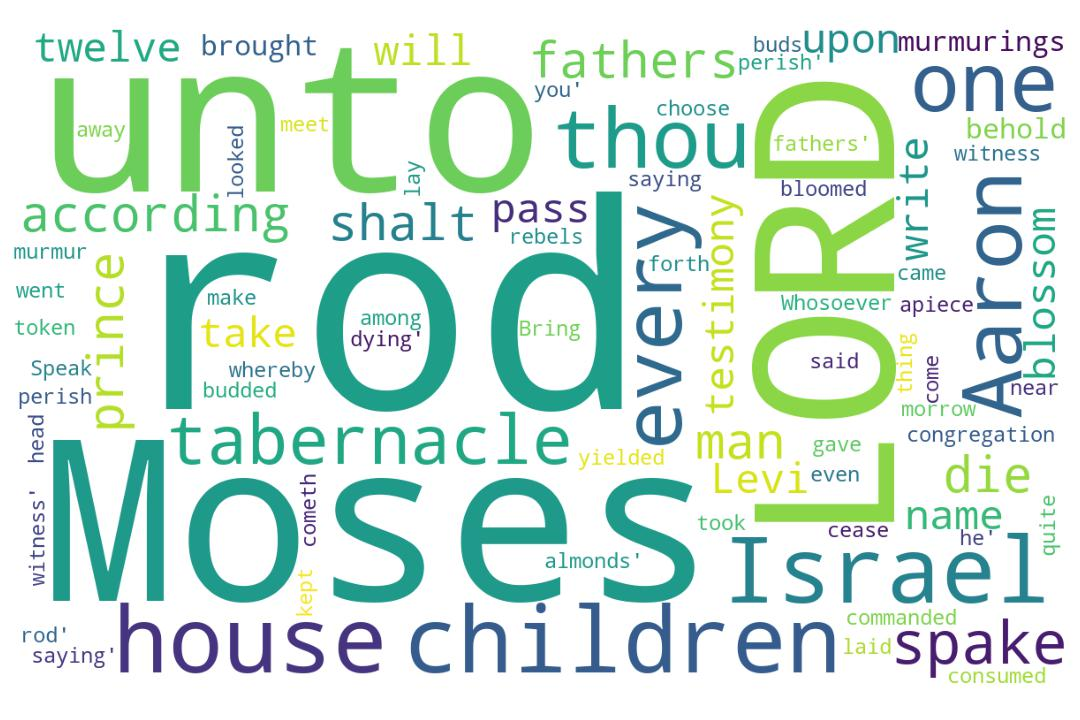
\includegraphics[width=\linewidth]{04OT-Numbers/Numbers17-WordCloud.jpg}
  \caption{Numbers 17 Word Cloud}
  \label{fig:Numbers 17 word Cloud}
\end{figure}

\marginpar{\scriptsize \centering \fcolorbox{bone}{lime}{\textbf{SHHHH}}\\ (Numbers 17:1-13) \begin{compactenum}[I.][8]
    \item  \textbf{Placement} \index[scripture]{Numbers!Num 17:04} (Numbers 17:4) 
    \item  \textbf{Purpose} \index[scripture]{Numbers!Num 17:05} (Numbers 17:5) 
    \item  \textbf{Princes} \index[scripture]{Numbers!Num 17:06} (Numbers 17:6) 
    \item  \textbf{Presence} \index[scripture]{Numbers!Num 17:07} (Numbers 17:7) 
    \item  \textbf{Prevention} \index[scripture]{Numbers!Num 17:10} (Numbers 17:10) 
    \item  \textbf{Perishing} \index[scripture]{Numbers!Num 17:12} (Numbers 17:12) 
    \item  \textbf{Pruning} %\index[scripture]{Numbers!Num 17:12} (Numbers 17:12) 
\end{compactenum}}
    



\footnote{\textcolor[cmyk]{0.99998,1,0,0}{\hyperlink{TOC}{Return to end of Table of Contents.}}}\footnote{\href{https://audiobible.com/bible/numbers_17.html}{\textcolor[cmyk]{0.99998,1,0,0}{Numbers 17 Audio}}}\textcolor[cmyk]{0.99998,1,0,0}{And the LORD spake unto Moses, saying,}
[2] \textcolor[cmyk]{0.99998,1,0,0}{Speak unto the children of Israel, and take of every one of them a rod according to the house of \emph{their} fathers, of all their princes according to the house of their fathers twelve rods: write thou every man's name upon his rod.}
[3] \textcolor[cmyk]{0.99998,1,0,0}{And thou shalt write Aaron's name upon the rod of Levi: for one rod \emph{shall} \emph{be} for the head of the house of their fathers.}
[4] \textcolor[cmyk]{0.99998,1,0,0}{And thou shalt lay them up \fcolorbox{bone}{lime}{in the tabernacle} of the congregation before the testimony, where I will meet with you.}
[5] \textcolor[cmyk]{0.99998,1,0,0}{And it shall come to pass, \emph{that} the man's rod, whom I shall choose, \fcolorbox{bone}{lime}{shall blossom}: and I will make to cease from me the murmurings of the children of Israel, whereby they murmur against you.}\\
\\
\P \textcolor[cmyk]{0.99998,1,0,0}{And Moses spake unto the children of Israel, and every one of their \fcolorbox{bone}{lime}{princes} gave him a rod apiece, for each prince one, according to their fathers' houses, \emph{even} twelve rods: and the rod of Aaron \emph{was} among their rods.}
[7] \textcolor[cmyk]{0.99998,1,0,0}{And Moses laid up the rods \fcolorbox{bone}{lime}{before the LORD} in the tabernacle of witness.}
[8] \textcolor[cmyk]{0.99998,1,0,0}{And it came to pass, that on the morrow Moses went into the tabernacle of witness; and, behold, the rod of Aaron for the house of Levi was budded, and brought forth buds, and bloomed blossoms, and yielded almonds.}\footnote{\textbf{Hebrews 9:4} - Which had the golden censer, and the ark of the covenant overlaid round about with gold, wherein was the golden pot that had manna, and Aaron’s rod that budded, and the tables of the covenant;}
[9] \textcolor[cmyk]{0.99998,1,0,0}{And Moses brought out all the rods from before the LORD unto all the children of Israel: and they looked, and took every man his rod.}\\
\\
\P \textcolor[cmyk]{0.99998,1,0,0}{And the LORD said unto Moses, Bring Aaron's rod again before the testimony, to be kept for a token \fcolorbox{bone}{lime}{against the rebels}; and thou shalt quite take away their murmurings from me, that they die not.}
[11] \textcolor[cmyk]{0.99998,1,0,0}{And Moses did \emph{so}: as the LORD commanded him, so did he.}
[12] \textcolor[cmyk]{0.99998,1,0,0}{And the children of Israel spake unto Moses, saying, Behold, we die, we \fcolorbox{bone}{lime}{perish}, we all perish.}
[13] \textcolor[cmyk]{0.99998,1,0,0}{Whosoever cometh any thing near unto the tabernacle of the LORD shall die: shall we be consumed with dying?}
\index[NWIV]{7!Numbers!Num 17:1}\index[AWIP]{And!Numbers!Num 17:1}\index[AWIP]{the!Numbers!Num 17:1}\index[AWIP]{LORD!Numbers!Num 17:1}\index[AWIP]{spake!Numbers!Num 17:1}\index[AWIP]{unto!Numbers!Num 17:1}\index[AWIP]{Moses!Numbers!Num 17:1}\index[AWIP]{saying!Numbers!Num 17:1}

\index[NWIV]{43!Numbers!Num 17:2}\index[AWIP]{Speak!Numbers!Num 17:2}\index[AWIP]{unto!Numbers!Num 17:2}\index[AWIP]{the!Numbers!Num 17:2}\index[AWIP]{the!Numbers!Num 17:2 (2)}\index[AWIP]{the!Numbers!Num 17:2 (3)}\index[AWIP]{children!Numbers!Num 17:2}\index[AWIP]{of!Numbers!Num 17:2}\index[AWIP]{of!Numbers!Num 17:2 (2)}\index[AWIP]{of!Numbers!Num 17:2 (3)}\index[AWIP]{of!Numbers!Num 17:2 (4)}\index[AWIP]{of!Numbers!Num 17:2 (5)}\index[AWIP]{of!Numbers!Num 17:2 (6)}\index[AWIP]{Israel!Numbers!Num 17:2}\index[AWIP]{and!Numbers!Num 17:2}\index[AWIP]{take!Numbers!Num 17:2}\index[AWIP]{every!Numbers!Num 17:2}\index[AWIP]{every!Numbers!Num 17:2 (2)}\index[AWIP]{one!Numbers!Num 17:2}\index[AWIP]{them!Numbers!Num 17:2}\index[AWIP]{a!Numbers!Num 17:2}\index[AWIP]{rod!Numbers!Num 17:2}\index[AWIP]{rod!Numbers!Num 17:2 (2)}\index[AWIP]{according!Numbers!Num 17:2}\index[AWIP]{according!Numbers!Num 17:2 (2)}\index[AWIP]{to!Numbers!Num 17:2}\index[AWIP]{to!Numbers!Num 17:2 (2)}\index[AWIP]{house!Numbers!Num 17:2}\index[AWIP]{house!Numbers!Num 17:2 (2)}\index[AWIP]{\emph{their}!Numbers!Num 17:2}\index[AWIP]{fathers!Numbers!Num 17:2}\index[AWIP]{fathers!Numbers!Num 17:2 (2)}\index[AWIP]{all!Numbers!Num 17:2}\index[AWIP]{their!Numbers!Num 17:2}\index[AWIP]{their!Numbers!Num 17:2 (2)}\index[AWIP]{princes!Numbers!Num 17:2}\index[AWIP]{twelve!Numbers!Num 17:2}\index[AWIP]{rods!Numbers!Num 17:2}\index[AWIP]{write!Numbers!Num 17:2}\index[AWIP]{thou!Numbers!Num 17:2}\index[AWIP]{man's!Numbers!Num 17:2}\index[AWIP]{name!Numbers!Num 17:2}\index[AWIP]{upon!Numbers!Num 17:2}\index[AWIP]{his!Numbers!Num 17:2}\index[AWIP]{\emph{their}!Numbers!Num 17:2}

\index[NWIV]{25!Numbers!Num 17:3}\index[AWIP]{And!Numbers!Num 17:3}\index[AWIP]{thou!Numbers!Num 17:3}\index[AWIP]{shalt!Numbers!Num 17:3}\index[AWIP]{write!Numbers!Num 17:3}\index[AWIP]{Aaron's!Numbers!Num 17:3}\index[AWIP]{name!Numbers!Num 17:3}\index[AWIP]{upon!Numbers!Num 17:3}\index[AWIP]{the!Numbers!Num 17:3}\index[AWIP]{the!Numbers!Num 17:3 (2)}\index[AWIP]{the!Numbers!Num 17:3 (3)}\index[AWIP]{rod!Numbers!Num 17:3}\index[AWIP]{rod!Numbers!Num 17:3 (2)}\index[AWIP]{of!Numbers!Num 17:3}\index[AWIP]{of!Numbers!Num 17:3 (2)}\index[AWIP]{of!Numbers!Num 17:3 (3)}\index[AWIP]{Levi!Numbers!Num 17:3}\index[AWIP]{for!Numbers!Num 17:3}\index[AWIP]{for!Numbers!Num 17:3 (2)}\index[AWIP]{one!Numbers!Num 17:3}\index[AWIP]{\emph{shall}!Numbers!Num 17:3}\index[AWIP]{\emph{be}!Numbers!Num 17:3}\index[AWIP]{head!Numbers!Num 17:3}\index[AWIP]{house!Numbers!Num 17:3}\index[AWIP]{their!Numbers!Num 17:3}\index[AWIP]{fathers!Numbers!Num 17:3}\index[AWIP]{\emph{shall}!Numbers!Num 17:3}\index[AWIP]{\emph{be}!Numbers!Num 17:3}

\index[NWIV]{21!Numbers!Num 17:4}\index[AWIP]{And!Numbers!Num 17:4}\index[AWIP]{thou!Numbers!Num 17:4}\index[AWIP]{shalt!Numbers!Num 17:4}\index[AWIP]{lay!Numbers!Num 17:4}\index[AWIP]{them!Numbers!Num 17:4}\index[AWIP]{up!Numbers!Num 17:4}\index[AWIP]{in!Numbers!Num 17:4}\index[AWIP]{the!Numbers!Num 17:4}\index[AWIP]{the!Numbers!Num 17:4 (2)}\index[AWIP]{the!Numbers!Num 17:4 (3)}\index[AWIP]{tabernacle!Numbers!Num 17:4}\index[AWIP]{of!Numbers!Num 17:4}\index[AWIP]{congregation!Numbers!Num 17:4}\index[AWIP]{before!Numbers!Num 17:4}\index[AWIP]{testimony!Numbers!Num 17:4}\index[AWIP]{where!Numbers!Num 17:4}\index[AWIP]{I!Numbers!Num 17:4}\index[AWIP]{will!Numbers!Num 17:4}\index[AWIP]{meet!Numbers!Num 17:4}\index[AWIP]{with!Numbers!Num 17:4}\index[AWIP]{you!Numbers!Num 17:4}

\index[NWIV]{36!Numbers!Num 17:5}\index[AWIP]{And!Numbers!Num 17:5}\index[AWIP]{it!Numbers!Num 17:5}\index[AWIP]{shall!Numbers!Num 17:5}\index[AWIP]{shall!Numbers!Num 17:5 (2)}\index[AWIP]{shall!Numbers!Num 17:5 (3)}\index[AWIP]{come!Numbers!Num 17:5}\index[AWIP]{to!Numbers!Num 17:5}\index[AWIP]{to!Numbers!Num 17:5 (2)}\index[AWIP]{pass!Numbers!Num 17:5}\index[AWIP]{\emph{that}!Numbers!Num 17:5}\index[AWIP]{the!Numbers!Num 17:5}\index[AWIP]{the!Numbers!Num 17:5 (2)}\index[AWIP]{the!Numbers!Num 17:5 (3)}\index[AWIP]{man's!Numbers!Num 17:5}\index[AWIP]{rod!Numbers!Num 17:5}\index[AWIP]{whom!Numbers!Num 17:5}\index[AWIP]{I!Numbers!Num 17:5}\index[AWIP]{I!Numbers!Num 17:5 (2)}\index[AWIP]{choose!Numbers!Num 17:5}\index[AWIP]{blossom!Numbers!Num 17:5}\index[AWIP]{and!Numbers!Num 17:5}\index[AWIP]{will!Numbers!Num 17:5}\index[AWIP]{make!Numbers!Num 17:5}\index[AWIP]{cease!Numbers!Num 17:5}\index[AWIP]{from!Numbers!Num 17:5}\index[AWIP]{me!Numbers!Num 17:5}\index[AWIP]{murmurings!Numbers!Num 17:5}\index[AWIP]{of!Numbers!Num 17:5}\index[AWIP]{of!Numbers!Num 17:5 (2)}\index[AWIP]{children!Numbers!Num 17:5}\index[AWIP]{Israel!Numbers!Num 17:5}\index[AWIP]{whereby!Numbers!Num 17:5}\index[AWIP]{they!Numbers!Num 17:5}\index[AWIP]{murmur!Numbers!Num 17:5}\index[AWIP]{against!Numbers!Num 17:5}\index[AWIP]{you!Numbers!Num 17:5}\index[AWIP]{\emph{that}!Numbers!Num 17:5}

\index[NWIV]{40!Numbers!Num 17:6}\index[AWIP]{And!Numbers!Num 17:6}\index[AWIP]{Moses!Numbers!Num 17:6}\index[AWIP]{spake!Numbers!Num 17:6}\index[AWIP]{unto!Numbers!Num 17:6}\index[AWIP]{the!Numbers!Num 17:6}\index[AWIP]{the!Numbers!Num 17:6 (2)}\index[AWIP]{children!Numbers!Num 17:6}\index[AWIP]{of!Numbers!Num 17:6}\index[AWIP]{of!Numbers!Num 17:6 (2)}\index[AWIP]{of!Numbers!Num 17:6 (3)}\index[AWIP]{Israel!Numbers!Num 17:6}\index[AWIP]{and!Numbers!Num 17:6}\index[AWIP]{and!Numbers!Num 17:6 (2)}\index[AWIP]{every!Numbers!Num 17:6}\index[AWIP]{one!Numbers!Num 17:6}\index[AWIP]{one!Numbers!Num 17:6 (2)}\index[AWIP]{their!Numbers!Num 17:6}\index[AWIP]{their!Numbers!Num 17:6 (2)}\index[AWIP]{their!Numbers!Num 17:6 (3)}\index[AWIP]{princes!Numbers!Num 17:6}\index[AWIP]{gave!Numbers!Num 17:6}\index[AWIP]{him!Numbers!Num 17:6}\index[AWIP]{a!Numbers!Num 17:6}\index[AWIP]{rod!Numbers!Num 17:6}\index[AWIP]{rod!Numbers!Num 17:6 (2)}\index[AWIP]{apiece!Numbers!Num 17:6}\index[AWIP]{for!Numbers!Num 17:6}\index[AWIP]{each!Numbers!Num 17:6}\index[AWIP]{prince!Numbers!Num 17:6}\index[AWIP]{according!Numbers!Num 17:6}\index[AWIP]{to!Numbers!Num 17:6}\index[AWIP]{fathers'!Numbers!Num 17:6}\index[AWIP]{houses!Numbers!Num 17:6}\index[AWIP]{\emph{even}!Numbers!Num 17:6}\index[AWIP]{twelve!Numbers!Num 17:6}\index[AWIP]{rods!Numbers!Num 17:6}\index[AWIP]{rods!Numbers!Num 17:6 (2)}\index[AWIP]{Aaron!Numbers!Num 17:6}\index[AWIP]{\emph{was}!Numbers!Num 17:6}\index[AWIP]{among!Numbers!Num 17:6}\index[AWIP]{\emph{even}!Numbers!Num 17:6}\index[AWIP]{\emph{was}!Numbers!Num 17:6}

\index[NWIV]{14!Numbers!Num 17:7}\index[AWIP]{And!Numbers!Num 17:7}\index[AWIP]{Moses!Numbers!Num 17:7}\index[AWIP]{laid!Numbers!Num 17:7}\index[AWIP]{up!Numbers!Num 17:7}\index[AWIP]{the!Numbers!Num 17:7}\index[AWIP]{the!Numbers!Num 17:7 (2)}\index[AWIP]{the!Numbers!Num 17:7 (3)}\index[AWIP]{rods!Numbers!Num 17:7}\index[AWIP]{before!Numbers!Num 17:7}\index[AWIP]{LORD!Numbers!Num 17:7}\index[AWIP]{in!Numbers!Num 17:7}\index[AWIP]{tabernacle!Numbers!Num 17:7}\index[AWIP]{of!Numbers!Num 17:7}\index[AWIP]{witness!Numbers!Num 17:7}

\index[NWIV]{39!Numbers!Num 17:8}\index[AWIP]{And!Numbers!Num 17:8}\index[AWIP]{it!Numbers!Num 17:8}\index[AWIP]{came!Numbers!Num 17:8}\index[AWIP]{to!Numbers!Num 17:8}\index[AWIP]{pass!Numbers!Num 17:8}\index[AWIP]{that!Numbers!Num 17:8}\index[AWIP]{on!Numbers!Num 17:8}\index[AWIP]{the!Numbers!Num 17:8}\index[AWIP]{the!Numbers!Num 17:8 (2)}\index[AWIP]{the!Numbers!Num 17:8 (3)}\index[AWIP]{the!Numbers!Num 17:8 (4)}\index[AWIP]{morrow!Numbers!Num 17:8}\index[AWIP]{Moses!Numbers!Num 17:8}\index[AWIP]{went!Numbers!Num 17:8}\index[AWIP]{into!Numbers!Num 17:8}\index[AWIP]{tabernacle!Numbers!Num 17:8}\index[AWIP]{of!Numbers!Num 17:8}\index[AWIP]{of!Numbers!Num 17:8 (2)}\index[AWIP]{of!Numbers!Num 17:8 (3)}\index[AWIP]{witness!Numbers!Num 17:8}\index[AWIP]{and!Numbers!Num 17:8}\index[AWIP]{and!Numbers!Num 17:8 (2)}\index[AWIP]{and!Numbers!Num 17:8 (3)}\index[AWIP]{and!Numbers!Num 17:8 (4)}\index[AWIP]{behold!Numbers!Num 17:8}\index[AWIP]{rod!Numbers!Num 17:8}\index[AWIP]{Aaron!Numbers!Num 17:8}\index[AWIP]{for!Numbers!Num 17:8}\index[AWIP]{house!Numbers!Num 17:8}\index[AWIP]{Levi!Numbers!Num 17:8}\index[AWIP]{was!Numbers!Num 17:8}\index[AWIP]{budded!Numbers!Num 17:8}\index[AWIP]{brought!Numbers!Num 17:8}\index[AWIP]{forth!Numbers!Num 17:8}\index[AWIP]{buds!Numbers!Num 17:8}\index[AWIP]{bloomed!Numbers!Num 17:8}\index[AWIP]{blossoms!Numbers!Num 17:8}\index[AWIP]{yielded!Numbers!Num 17:8}\index[AWIP]{almonds!Numbers!Num 17:8}

\index[NWIV]{26!Numbers!Num 17:9}\index[AWIP]{And!Numbers!Num 17:9}\index[AWIP]{Moses!Numbers!Num 17:9}\index[AWIP]{brought!Numbers!Num 17:9}\index[AWIP]{out!Numbers!Num 17:9}\index[AWIP]{all!Numbers!Num 17:9}\index[AWIP]{all!Numbers!Num 17:9 (2)}\index[AWIP]{the!Numbers!Num 17:9}\index[AWIP]{the!Numbers!Num 17:9 (2)}\index[AWIP]{the!Numbers!Num 17:9 (3)}\index[AWIP]{rods!Numbers!Num 17:9}\index[AWIP]{from!Numbers!Num 17:9}\index[AWIP]{before!Numbers!Num 17:9}\index[AWIP]{LORD!Numbers!Num 17:9}\index[AWIP]{unto!Numbers!Num 17:9}\index[AWIP]{children!Numbers!Num 17:9}\index[AWIP]{of!Numbers!Num 17:9}\index[AWIP]{Israel!Numbers!Num 17:9}\index[AWIP]{and!Numbers!Num 17:9}\index[AWIP]{and!Numbers!Num 17:9 (2)}\index[AWIP]{they!Numbers!Num 17:9}\index[AWIP]{looked!Numbers!Num 17:9}\index[AWIP]{took!Numbers!Num 17:9}\index[AWIP]{every!Numbers!Num 17:9}\index[AWIP]{man!Numbers!Num 17:9}\index[AWIP]{his!Numbers!Num 17:9}\index[AWIP]{rod!Numbers!Num 17:9}

\index[NWIV]{36!Numbers!Num 17:10}\index[AWIP]{And!Numbers!Num 17:10}\index[AWIP]{the!Numbers!Num 17:10}\index[AWIP]{the!Numbers!Num 17:10 (2)}\index[AWIP]{the!Numbers!Num 17:10 (3)}\index[AWIP]{LORD!Numbers!Num 17:10}\index[AWIP]{said!Numbers!Num 17:10}\index[AWIP]{unto!Numbers!Num 17:10}\index[AWIP]{Moses!Numbers!Num 17:10}\index[AWIP]{Bring!Numbers!Num 17:10}\index[AWIP]{Aaron's!Numbers!Num 17:10}\index[AWIP]{rod!Numbers!Num 17:10}\index[AWIP]{again!Numbers!Num 17:10}\index[AWIP]{before!Numbers!Num 17:10}\index[AWIP]{testimony!Numbers!Num 17:10}\index[AWIP]{to!Numbers!Num 17:10}\index[AWIP]{be!Numbers!Num 17:10}\index[AWIP]{kept!Numbers!Num 17:10}\index[AWIP]{for!Numbers!Num 17:10}\index[AWIP]{a!Numbers!Num 17:10}\index[AWIP]{token!Numbers!Num 17:10}\index[AWIP]{against!Numbers!Num 17:10}\index[AWIP]{rebels!Numbers!Num 17:10}\index[AWIP]{and!Numbers!Num 17:10}\index[AWIP]{thou!Numbers!Num 17:10}\index[AWIP]{shalt!Numbers!Num 17:10}\index[AWIP]{quite!Numbers!Num 17:10}\index[AWIP]{take!Numbers!Num 17:10}\index[AWIP]{away!Numbers!Num 17:10}\index[AWIP]{their!Numbers!Num 17:10}\index[AWIP]{murmurings!Numbers!Num 17:10}\index[AWIP]{from!Numbers!Num 17:10}\index[AWIP]{me!Numbers!Num 17:10}\index[AWIP]{that!Numbers!Num 17:10}\index[AWIP]{they!Numbers!Num 17:10}\index[AWIP]{die!Numbers!Num 17:10}\index[AWIP]{not!Numbers!Num 17:10}

\index[NWIV]{12!Numbers!Num 17:11}\index[AWIP]{And!Numbers!Num 17:11}\index[AWIP]{Moses!Numbers!Num 17:11}\index[AWIP]{did!Numbers!Num 17:11}\index[AWIP]{did!Numbers!Num 17:11 (2)}\index[AWIP]{\emph{so}!Numbers!Num 17:11}\index[AWIP]{as!Numbers!Num 17:11}\index[AWIP]{the!Numbers!Num 17:11}\index[AWIP]{LORD!Numbers!Num 17:11}\index[AWIP]{commanded!Numbers!Num 17:11}\index[AWIP]{him!Numbers!Num 17:11}\index[AWIP]{so!Numbers!Num 17:11}\index[AWIP]{he!Numbers!Num 17:11}\index[AWIP]{\emph{so}!Numbers!Num 17:11}

\index[NWIV]{17!Numbers!Num 17:12}\index[AWIP]{And!Numbers!Num 17:12}\index[AWIP]{the!Numbers!Num 17:12}\index[AWIP]{children!Numbers!Num 17:12}\index[AWIP]{of!Numbers!Num 17:12}\index[AWIP]{Israel!Numbers!Num 17:12}\index[AWIP]{spake!Numbers!Num 17:12}\index[AWIP]{unto!Numbers!Num 17:12}\index[AWIP]{Moses!Numbers!Num 17:12}\index[AWIP]{saying!Numbers!Num 17:12}\index[AWIP]{Behold!Numbers!Num 17:12}\index[AWIP]{we!Numbers!Num 17:12}\index[AWIP]{we!Numbers!Num 17:12 (2)}\index[AWIP]{we!Numbers!Num 17:12 (3)}\index[AWIP]{die!Numbers!Num 17:12}\index[AWIP]{perish!Numbers!Num 17:12}\index[AWIP]{perish!Numbers!Num 17:12 (2)}\index[AWIP]{all!Numbers!Num 17:12}

\index[NWIV]{19!Numbers!Num 17:13}\index[AWIP]{Whosoever!Numbers!Num 17:13}\index[AWIP]{cometh!Numbers!Num 17:13}\index[AWIP]{any!Numbers!Num 17:13}\index[AWIP]{thing!Numbers!Num 17:13}\index[AWIP]{near!Numbers!Num 17:13}\index[AWIP]{unto!Numbers!Num 17:13}\index[AWIP]{the!Numbers!Num 17:13}\index[AWIP]{the!Numbers!Num 17:13 (2)}\index[AWIP]{tabernacle!Numbers!Num 17:13}\index[AWIP]{of!Numbers!Num 17:13}\index[AWIP]{LORD!Numbers!Num 17:13}\index[AWIP]{shall!Numbers!Num 17:13}\index[AWIP]{shall!Numbers!Num 17:13 (2)}\index[AWIP]{die!Numbers!Num 17:13}\index[AWIP]{we!Numbers!Num 17:13}\index[AWIP]{be!Numbers!Num 17:13}\index[AWIP]{consumed!Numbers!Num 17:13}\index[AWIP]{with!Numbers!Num 17:13}\index[AWIP]{dying?!Numbers!Num 17:13}


\section{Number 17 Outlines}

\subsection{My Outlines}

\subsubsection{Shhhhh}
%Practical Wisdom from Proverbs 6:\footnote{03 November 2014, Keith Anthony}
\index[speaker]{Keith Anthony!Numbers 17 (Shhhhh}
\index[series]{Numbers (Keith Anthony)!Numbers 17 (Shhhhh)}
\index[date]{2018/02/15!Numbers 17 (Shhhhh (Keith Anthony)
(Keith Anthony)}
\begin{compactenum}[I.]
    \item  \textbf{Placement} \index[scripture]{Numbers!Num 17:04} (Numbers 17:4) 
    \item  \textbf{Purpose} \index[scripture]{Numbers!Num 17:05} (Numbers 17:5) 
    \item  \textbf{Princes} \index[scripture]{Numbers!Num 17:06} (Numbers 17:6) 
    \item  \textbf{Presence} \index[scripture]{Numbers!Num 17:07} (Numbers 17:7) 
    \item  \textbf{Prevention} \index[scripture]{Numbers!Num 17:10} (Numbers 17:10) 
    \item  \textbf{Perishing} \index[scripture]{Numbers!Num 17:12} (Numbers 17:12) 
    \item  \textbf{Pruning} %\index[scripture]{Numbers!Num 17:12} (Numbers 17:12) 
\end{compactenum}





\subsection{Outlines from Others}
\section{Numbers 17 Comments}


\subsection{Numbers 17 Repeated Phrases}


%%%%%%%%%%
%%%%%%%%%%
\normalsize
 
\begin{center}
\begin{longtable}{|c|c|}
\caption[Numbers 17 Repeated Phrases]{Numbers 17 Repeated Phrases}\label{table:Repeated Phrases Numbers 17} \\
\hline \multicolumn{1}{|c|}{\textbf{Phrase}} & \multicolumn{1}{c|}{\textbf{Frequency}} \\ \hline 
\endfirsthead
 
\multicolumn{2}{c}
{{\bfseries \tablename\ \thetable{} -- continued from previous page}} \\  
\hline \multicolumn{1}{|c|}{\textbf{Phrase}} & \multicolumn{1}{c|}{\textbf{Frequency}} \\ \hline 
\endhead
 
\hline \multicolumn{2}{c}{{ }} \\ \hline
\endfoot 
the LORD & 6\\ \hline 
the children & 5\\ \hline 
the children of & 5\\ \hline 
the children of Israel & 5\\ \hline 
children of & 5\\ \hline 
children of Israel & 5\\ \hline 
of Israel & 5\\ \hline 
the house & 4\\ \hline 
the house of & 4\\ \hline 
house of & 4\\ \hline 
of the & 4\\ \hline 
the tabernacle & 4\\ \hline 
the tabernacle of & 4\\ \hline 
tabernacle of & 4\\ \hline 
before the & 4\\ \hline 
And Moses & 4\\ \hline 
And the & 3\\ \hline 
spake unto & 3\\ \hline 
unto Moses & 3\\ \hline 
unto the & 3\\ \hline 
the children of Israel and & 3\\ \hline 
children of Israel and & 3\\ \hline 
of Israel and & 3\\ \hline 
Israel and & 3\\ \hline 
according to & 3\\ \hline 
of their & 3\\ \hline 
thou shalt & 3\\ \hline 
the rod & 3\\ \hline 
the rod of & 3\\ \hline 
rod of & 3\\ \hline 
\end{longtable}
\end{center}



%%%%%%%%%%
%%%%%%%%%%



\section{Numbers 17 Statistics}

%%%%%%%%%%%%%%%%%%%%%%%%%%%
%%%%% Word Statistics
%%%%%%%%%%%%%%%%%%%%%%%%%%


\normalsize



\subsection{Chapter Word Statistics}


%%%%%%%%%%
%%%%%%%%%%
 
\begin{center}
\begin{longtable}{l|c|c|c|c}
\caption[Stats for Numbers 17]{Stats for Numbers 17} \label{table:Stats for Numbers 17} \\ 
\hline \multicolumn{1}{|c|}{\textbf{Verse(s)}} & \multicolumn{1}{|c|}{\textbf{Count}} & \multicolumn{1}{|c|}{\textbf{Unique}} & \multicolumn{1}{|c|}{\textbf{Italics}} & \multicolumn{1}{|c|}{\textbf{Uniq Italic}}  \\ \hline 
\endfirsthead
 
\multicolumn{5}{c}
{{\bfseries \tablename\ \thetable{} -- continued from previous page}} \\  
\hline \multicolumn{1}{|c|}{\textbf{Verse(s)}} & \multicolumn{1}{|c|}{\textbf{Count}} & \multicolumn{1}{|c|}{\textbf{Unique}} & \multicolumn{1}{|c|}{\textbf{Italics}} & \multicolumn{1}{|c|}{\textbf{Uniq Italic}}  \\ \hline 
\endhead
 
\hline \multicolumn{5}{|r|}{{Continued if needed}} \\ \hline
\endfoot 
1 & 7 & 7 & 0 & 0\\ \hline
2 & 43 & 29 & 1 & 1\\ \hline
3 & 25 & 19 & 2 & 2\\ \hline
4 & 21 & 19 & 0 & 0\\ \hline
5 & 36 & 29 & 1 & 1\\ \hline
6 & 40 & 31 & 2 & 2\\ \hline
7 & 14 & 12 & 0 & 0\\ \hline
8 & 39 & 31 & 0 & 0\\ \hline
9 & 26 & 22 & 0 & 0\\ \hline
10 & 36 & 34 & 0 & 0\\ \hline
11 & 12 & 11 & 1 & 1\\ \hline
12 & 17 & 14 & 0 & 0\\ \hline
13 & 19 & 17 & 0 & 0\\ \hline
\hline \hline
Total & 335 & 131 & 7 & 7



\end{longtable}
\end{center}

%%%%%%%%%%
%%%%%%%%%%
 
\subsection{Words by Frequency}

\begin{center}
\begin{longtable}{l|r}
\caption[Word Frequencies in Numbers 17]{Word Frequencies in Numbers 17} \label{table:WordsIn-Numbers-17} \\ 
\hline \multicolumn{1}{|c|}{\textbf{Word}} & \multicolumn{1}{c|}{\textbf{Frequency}} \\ \hline 
\endfirsthead
 
\multicolumn{2}{c}
{{\bfseries \tablename\ \thetable{} -- continued from previous page}} \\ 
\hline \multicolumn{1}{|c|}{\textbf{Word}} & \multicolumn{1}{c|}{\textbf{Frequency}} \\ \hline 
\endhead
 
\hline \multicolumn{2}{|r|}{{Continued if needed}} \\ \hline
\endfoot
 
\hline \hline
\endlastfoot
the & 32 \\ \hline
of & 22 \\ \hline
And & 11 \\ \hline
and & 11 \\ \hline
rod & 10 \\ \hline
Moses & 8 \\ \hline
unto & 7 \\ \hline
to & 7 \\ \hline
their & 7 \\ \hline
LORD & 6 \\ \hline
children & 5 \\ \hline
Israel & 5 \\ \hline
rods & 5 \\ \hline
for & 5 \\ \hline
shall & 5 \\ \hline
every & 4 \\ \hline
one & 4 \\ \hline
house & 4 \\ \hline
all & 4 \\ \hline
thou & 4 \\ \hline
tabernacle & 4 \\ \hline
before & 4 \\ \hline
we & 4 \\ \hline
spake & 3 \\ \hline
a & 3 \\ \hline
according & 3 \\ \hline
fathers & 3 \\ \hline
shalt & 3 \\ \hline
I & 3 \\ \hline
from & 3 \\ \hline
they & 3 \\ \hline
die & 3 \\ \hline
saying & 2 \\ \hline
take & 2 \\ \hline
them & 2 \\ \hline
princes & 2 \\ \hline
twelve & 2 \\ \hline
write & 2 \\ \hline
man's & 2 \\ \hline
name & 2 \\ \hline
upon & 2 \\ \hline
his & 2 \\ \hline
Aaron's & 2 \\ \hline
Levi & 2 \\ \hline
up & 2 \\ \hline
in & 2 \\ \hline
testimony & 2 \\ \hline
will & 2 \\ \hline
with & 2 \\ \hline
you & 2 \\ \hline
it & 2 \\ \hline
pass & 2 \\ \hline
me & 2 \\ \hline
murmurings & 2 \\ \hline
against & 2 \\ \hline
him & 2 \\ \hline
Aaron & 2 \\ \hline
witness & 2 \\ \hline
that & 2 \\ \hline
brought & 2 \\ \hline
be & 2 \\ \hline
did & 2 \\ \hline
perish & 2 \\ \hline
Speak & 1 \\ \hline
\emph{their} & 1 \\ \hline
\emph{shall} & 1 \\ \hline
\emph{be} & 1 \\ \hline
head & 1 \\ \hline
lay & 1 \\ \hline
congregation & 1 \\ \hline
where & 1 \\ \hline
meet & 1 \\ \hline
come & 1 \\ \hline
\emph{that} & 1 \\ \hline
whom & 1 \\ \hline
choose & 1 \\ \hline
blossom & 1 \\ \hline
make & 1 \\ \hline
cease & 1 \\ \hline
whereby & 1 \\ \hline
murmur & 1 \\ \hline
gave & 1 \\ \hline
apiece & 1 \\ \hline
each & 1 \\ \hline
prince & 1 \\ \hline
fathers' & 1 \\ \hline
houses & 1 \\ \hline
\emph{even} & 1 \\ \hline
\emph{was} & 1 \\ \hline
among & 1 \\ \hline
laid & 1 \\ \hline
came & 1 \\ \hline
on & 1 \\ \hline
morrow & 1 \\ \hline
went & 1 \\ \hline
into & 1 \\ \hline
behold & 1 \\ \hline
was & 1 \\ \hline
budded & 1 \\ \hline
forth & 1 \\ \hline
buds & 1 \\ \hline
bloomed & 1 \\ \hline
blossoms & 1 \\ \hline
yielded & 1 \\ \hline
almonds & 1 \\ \hline
out & 1 \\ \hline
looked & 1 \\ \hline
took & 1 \\ \hline
man & 1 \\ \hline
said & 1 \\ \hline
Bring & 1 \\ \hline
again & 1 \\ \hline
kept & 1 \\ \hline
token & 1 \\ \hline
rebels & 1 \\ \hline
quite & 1 \\ \hline
away & 1 \\ \hline
not & 1 \\ \hline
\emph{so} & 1 \\ \hline
as & 1 \\ \hline
commanded & 1 \\ \hline
so & 1 \\ \hline
he & 1 \\ \hline
Behold & 1 \\ \hline
Whosoever & 1 \\ \hline
cometh & 1 \\ \hline
any & 1 \\ \hline
thing & 1 \\ \hline
near & 1 \\ \hline
consumed & 1 \\ \hline
dying & 1 \\ \hline
\end{longtable}
\end{center}



\normalsize



\subsection{Words Alphabetically}

\begin{center}
\begin{longtable}{l|r}
\caption[Word Alphabetically in Numbers 17]{Word Alphabetically in Numbers 17} \label{table:WordsIn-Numbers-17} \\ 
\hline \multicolumn{1}{|c|}{\textbf{Word}} & \multicolumn{1}{c|}{\textbf{Frequency}} \\ \hline 
\endfirsthead
 
\multicolumn{2}{c}
{{\bfseries \tablename\ \thetable{} -- continued from previous page}} \\ 
\hline \multicolumn{1}{|c|}{\textbf{Word}} & \multicolumn{1}{c|}{\textbf{Frequency}} \\ \hline 
\endhead
 
\hline \multicolumn{2}{|r|}{{Continued if needed}} \\ \hline
\endfoot
 
\hline \hline
\endlastfoot
Aaron & 2 \\ \hline
Aaron's & 2 \\ \hline
And & 11 \\ \hline
Behold & 1 \\ \hline
Bring & 1 \\ \hline
I & 3 \\ \hline
Israel & 5 \\ \hline
LORD & 6 \\ \hline
Levi & 2 \\ \hline
Moses & 8 \\ \hline
Speak & 1 \\ \hline
Whosoever & 1 \\ \hline
\emph{be} & 1 \\ \hline
\emph{even} & 1 \\ \hline
\emph{shall} & 1 \\ \hline
\emph{so} & 1 \\ \hline
\emph{that} & 1 \\ \hline
\emph{their} & 1 \\ \hline
\emph{was} & 1 \\ \hline
a & 3 \\ \hline
according & 3 \\ \hline
again & 1 \\ \hline
against & 2 \\ \hline
all & 4 \\ \hline
almonds & 1 \\ \hline
among & 1 \\ \hline
and & 11 \\ \hline
any & 1 \\ \hline
apiece & 1 \\ \hline
as & 1 \\ \hline
away & 1 \\ \hline
be & 2 \\ \hline
before & 4 \\ \hline
behold & 1 \\ \hline
bloomed & 1 \\ \hline
blossom & 1 \\ \hline
blossoms & 1 \\ \hline
brought & 2 \\ \hline
budded & 1 \\ \hline
buds & 1 \\ \hline
came & 1 \\ \hline
cease & 1 \\ \hline
children & 5 \\ \hline
choose & 1 \\ \hline
come & 1 \\ \hline
cometh & 1 \\ \hline
commanded & 1 \\ \hline
congregation & 1 \\ \hline
consumed & 1 \\ \hline
did & 2 \\ \hline
die & 3 \\ \hline
dying & 1 \\ \hline
each & 1 \\ \hline
every & 4 \\ \hline
fathers & 3 \\ \hline
fathers' & 1 \\ \hline
for & 5 \\ \hline
forth & 1 \\ \hline
from & 3 \\ \hline
gave & 1 \\ \hline
he & 1 \\ \hline
head & 1 \\ \hline
him & 2 \\ \hline
his & 2 \\ \hline
house & 4 \\ \hline
houses & 1 \\ \hline
in & 2 \\ \hline
into & 1 \\ \hline
it & 2 \\ \hline
kept & 1 \\ \hline
laid & 1 \\ \hline
lay & 1 \\ \hline
looked & 1 \\ \hline
make & 1 \\ \hline
man & 1 \\ \hline
man's & 2 \\ \hline
me & 2 \\ \hline
meet & 1 \\ \hline
morrow & 1 \\ \hline
murmur & 1 \\ \hline
murmurings & 2 \\ \hline
name & 2 \\ \hline
near & 1 \\ \hline
not & 1 \\ \hline
of & 22 \\ \hline
on & 1 \\ \hline
one & 4 \\ \hline
out & 1 \\ \hline
pass & 2 \\ \hline
perish & 2 \\ \hline
prince & 1 \\ \hline
princes & 2 \\ \hline
quite & 1 \\ \hline
rebels & 1 \\ \hline
rod & 10 \\ \hline
rods & 5 \\ \hline
said & 1 \\ \hline
saying & 2 \\ \hline
shall & 5 \\ \hline
shalt & 3 \\ \hline
so & 1 \\ \hline
spake & 3 \\ \hline
tabernacle & 4 \\ \hline
take & 2 \\ \hline
testimony & 2 \\ \hline
that & 2 \\ \hline
the & 32 \\ \hline
their & 7 \\ \hline
them & 2 \\ \hline
they & 3 \\ \hline
thing & 1 \\ \hline
thou & 4 \\ \hline
to & 7 \\ \hline
token & 1 \\ \hline
took & 1 \\ \hline
twelve & 2 \\ \hline
unto & 7 \\ \hline
up & 2 \\ \hline
upon & 2 \\ \hline
was & 1 \\ \hline
we & 4 \\ \hline
went & 1 \\ \hline
where & 1 \\ \hline
whereby & 1 \\ \hline
whom & 1 \\ \hline
will & 2 \\ \hline
with & 2 \\ \hline
witness & 2 \\ \hline
write & 2 \\ \hline
yielded & 1 \\ \hline
you & 2 \\ \hline
\end{longtable}
\end{center}



\normalsize



\subsection{Word Lengths in Chapter}
\normalsize
\begin{longtable}{l|p{3.75in}}
\caption[Words by Length in Numbers 17]{Words by Length in Numbers 17} \label{table:WordsIn-Numbers-17} \\ 
\hline \multicolumn{1}{|c|}{\textbf{Length}} & \multicolumn{1}{c|}{\textbf{Words}} \\ \hline 
\endfirsthead
 
\multicolumn{2}{c}
{{\bfseries \tablename\ \thetable{} -- continued from previous page}} \\ 
\hline \multicolumn{1}{|c|}{\textbf{Length}} & \multicolumn{1}{c|}{\textbf{Words}} \\ \hline 
\endhead
 
\hline \multicolumn{2}{|r|}{{Continued if needed}} \\ \hline
\endfoot
 
\hline \hline
\endlastfoot
1 & a, I \\ \hline
2 & of, to, \emph{be}, up, in, it, me, on, be, \emph{so}, as, so, he, we \\ \hline
3 & And, the, and, one, rod, all, his, for, lay, you, him, \emph{was}, was, out, man, die, not, did, any \\ \hline
4 & LORD, unto, take, them, rods, thou, name, upon, Levi, head, will, meet, with, come, pass, \emph{that}, whom, make, from, they, gave, each, \emph{even}, laid, came, that, went, into, buds, took, said, kept, away, near \\ \hline
5 & spake, Moses, Speak, every, house, \emph{their}, their, write, man's, shalt, \emph{shall}, where, shall, cease, Aaron, among, forth, Bring, again, token, quite, thing, dying \\ \hline
6 & saying, Israel, twelve, before, choose, murmur, apiece, prince, houses, morrow, behold, budded, looked, rebels, Behold, perish, cometh \\ \hline
7 & fathers, princes, Aaron's, blossom, whereby, against, witness, brought, bloomed, yielded, almonds \\ \hline
8 & children, fathers', blossoms, consumed \\ \hline
9 & according, testimony, commanded, Whosoever \\ \hline
10 & tabernacle, murmurings \\ \hline
12 & congregation \\ \hline
\end{longtable}






%%%%%%%%%%
%%%%%%%%%%

\chapter{Numbers 18}

\begin{figure}
  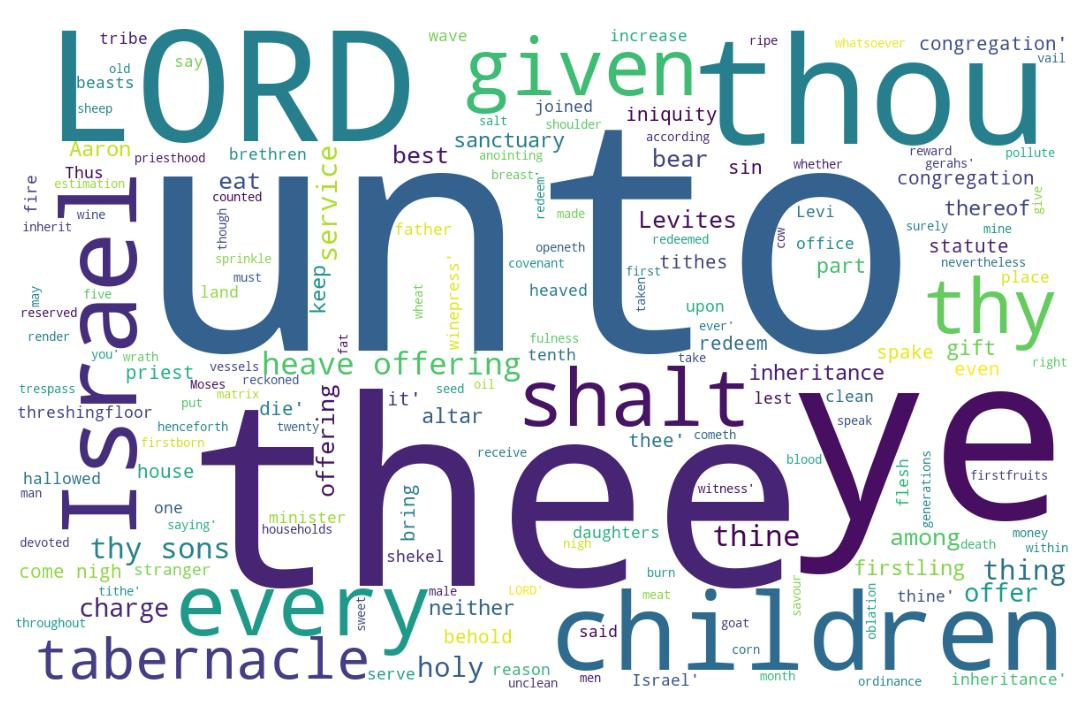
\includegraphics[width=\linewidth]{04OT-Numbers/Numbers18-WordCloud.jpg}
  \caption{Numbers 18 Word Cloud}
  \label{fig:Numbers 18 word Cloud}
\end{figure}


\marginpar{\scriptsize \centering \fcolorbox{bone}{lime}{\textbf{THE AARONIC PRIESTHOOD}}\\ (Numbers 18:1-32) \begin{compactenum}[I.][8]
    \item  \textbf{Sanctuary} \index[scripture]{Numbers!Num 18:01} \index[scripture]{Numbers!Num 18:03}\index[scripture]{Numbers!Num 18:05}\index[scripture]{Numbers!Num 18:16}(Numbers 18:1, 3, 5, 16) -- access to the sanctuary
    \item  \textbf{Sons} \index[scripture]{Numbers!Num 18:01} \index[scripture]{Numbers!Num 18:02}\index[scripture]{Numbers!Num 18:07}\index[scripture]{Numbers!Num 18:08}\index[scripture]{Numbers!Num 18:09}\index[scripture]{Numbers!Num 18:11}\index[scripture]{Numbers!Num 18:19} (Numbers 18:1, 2, 7, 8, 9, 11, 19) -- there is a family relationship between the priests. Here is the Aaronic priesthood. Elsewhere, see the priesthood of Melchisedek!
    \item  \textbf{Service} \index[scripture]{Numbers!Num 18:04} \index[scripture]{Numbers!Num 18:06}\index[scripture]{Numbers!Num 18:07}\index[scripture]{Numbers!Num 18:21}\index[scripture]{Numbers!Num 18:31}(Numbers 18:4, 6, 7, 21, 23, 31) -- the priests had duties of service
    \item  \textbf{Strangers} \index[scripture]{Numbers!Num 18:04} \index[scripture]{Numbers!Num 18:07}  (Numbers 18:4, 7) -- The strangers, people not part of God's fold, have no business with the priesthood
    \item  \textbf{Statutes} \index[scripture]{Numbers!Num 18:11} \index[scripture]{Numbers!Num 18:19}\index[scripture]{Numbers!Num 18:23} (Numbers 18:11, 19, 23) -- There are rules, God-given rules, for accessing and serving God
    \item  \textbf{Sin \& Sinners} \index[scripture]{Numbers!Num 18:09} \index[scripture]{Numbers!Num 18:22}\index[scripture]{Numbers!Num 18:26} \index[scripture]{Numbers!Num 18:32}(Numbers 18:9, 22, 26, 32) -- That sin problem -- always there to be dealt with
\end{compactenum}}
    




\footnote{\textcolor[cmyk]{0.99998,1,0,0}{\hyperlink{TOC}{Return to end of Table of Contents.}}}\footnote{\href{https://audiobible.com/bible/numbers_18.html}{\textcolor[cmyk]{0.99998,1,0,0}{Numbers 18 Audio}}}\textcolor[cmyk]{0.99998,1,0,0}{And the LORD said unto Aaron, Thou and thy \fcolorbox{bone}{lime}{sons} and thy father's house with thee shall bear the iniquity of the \fcolorbox{bone}{lime}{sanctuary}: and thou and thy sons with thee shall bear the iniquity of your priesthood.}
[2] \textcolor[cmyk]{0.99998,1,0,0}{And thy brethren also of the tribe of Levi, the tribe of thy father, bring thou with thee, that they may \fcolorbox{bone}{bone}{be} joined unto thee, and minister unto thee: but thou and thy \fcolorbox{bone}{lime}{sons} with thee \emph{shall} \emph{minister} before the tabernacle of witness.}
[3] \textcolor[cmyk]{0.99998,1,0,0}{And they shall keep thy charge, and the charge of all the tabernacle: only they shall not come nigh the vessels of the \fcolorbox{bone}{lime}{sanctuary} and the altar, that neither they, nor ye also, die.}
[4] \textcolor[cmyk]{0.99998,1,0,0}{And they shall \fcolorbox{bone}{bone}{be} joined unto thee, and keep the charge of the tabernacle of the congregation, for all the \fcolorbox{bone}{lime}{service} of the tabernacle: and \fcolorbox{bone}{bone}{a} \fcolorbox{bone}{lime}{stranger} shall not come nigh unto you.}
[5] \textcolor[cmyk]{0.99998,1,0,0}{And ye shall keep the charge of the \fcolorbox{bone}{lime}{sanctuary}, and the charge of the altar: that there \fcolorbox{bone}{bone}{be} no wrath any more upon \fcolorbox{bone}{bone}{the children of Israel}.}
[6] \textcolor[cmyk]{0.99998,1,0,0}{And \fcolorbox{bone}{bone}{I}, behold, \fcolorbox{bone}{bone}{I} have taken your brethren the Levites from among \fcolorbox{bone}{bone}{the children of Israel}: to you \emph{they} \emph{are} given \emph{as} \fcolorbox{bone}{bone}{a} gift for the LORD, to do the \fcolorbox{bone}{lime}{service} of the tabernacle of the congregation.}
[7] \textcolor[cmyk]{0.99998,1,0,0}{Therefore thou and thy \fcolorbox{bone}{lime}{sons} with thee shall keep your priest's office for every thing of the altar, and within the vail; and ye shall serve: \fcolorbox{bone}{bone}{I} have given your priest's office \emph{unto} \emph{you} as \fcolorbox{bone}{bone}{a} \fcolorbox{bone}{lime}{service} of gift: and the \fcolorbox{bone}{lime}{stranger} that cometh nigh shall \fcolorbox{bone}{bone}{be} put to death.}\\
\\
\P \textcolor[cmyk]{0.99998,1,0,0}{And the LORD spake unto Aaron, Behold, \fcolorbox{bone}{bone}{I} also have given thee the charge of mine heave offerings of all the hallowed things of \fcolorbox{bone}{bone}{the children of Israel}; unto thee have \fcolorbox{bone}{bone}{I} given them by reason of the anointing, and to thy \fcolorbox{bone}{lime}{sons}, by an ordinance for ever.}
[9] \textcolor[cmyk]{0.99998,1,0,0}{This shall \fcolorbox{bone}{bone}{be} thine of the most holy things, \emph{reserved} from the fire: every oblation of their's, every meat offering of their's, and every \fcolorbox{bone}{lime}{sin} offering of their's, and every trespass offering of their's, which they shall render unto me, \emph{shall} \emph{be} most holy for thee and for thy \fcolorbox{bone}{lime}{sons}.}
[10] \textcolor[cmyk]{0.99998,1,0,0}{In the most holy \emph{place} shalt thou eat it; every male shall eat it: it shall \fcolorbox{bone}{bone}{be} holy unto thee.}
[11] \textcolor[cmyk]{0.99998,1,0,0}{And this \emph{is} thine; the heave offering of their gift, with all the wave offerings of \fcolorbox{bone}{bone}{the children of Israel}: \fcolorbox{bone}{bone}{I} have given them unto thee, and to thy \fcolorbox{bone}{lime}{sons} and to thy daughters with thee, by \fcolorbox{bone}{bone}{a} \fcolorbox{bone}{lime}{statute} for ever: every one that is clean in thy house shall eat of it.}
[12] \textcolor[cmyk]{0.99998,1,0,0}{All the best of the oil, and all the best of the wine, and of the wheat, the firstfruits of them which they shall offer unto the LORD, them have \fcolorbox{bone}{bone}{I} given thee.}
[13] \textcolor[cmyk]{0.99998,1,0,0}{\emph{And} whatsoever is first ripe in the land, which they shall bring unto the LORD, shall \fcolorbox{bone}{bone}{be} thine; every one that is clean in thine house shall eat \emph{of} it.}
[14] \textcolor[cmyk]{0.99998,1,0,0}{Every thing devoted in Israel shall \fcolorbox{bone}{bone}{be} thine.}
[15] \textcolor[cmyk]{0.99998,1,0,0}{Every thing that openeth the matrix in all flesh, which they bring unto the LORD, \emph{whether} \emph{it} \emph{be} of men or beasts, shall \fcolorbox{bone}{bone}{be} thine: nevertheless the firstborn of man shalt thou surely redeem, and the firstling of unclean beasts shalt thou redeem.}
[16] \textcolor[cmyk]{0.99998,1,0,0}{And those that are to \fcolorbox{bone}{bone}{be} redeemed from \fcolorbox{bone}{bone}{a} month old shalt thou redeem, according to thine estimation, for the money of five shekels, after the shekel of the \fcolorbox{bone}{lime}{sanctuary}, which \emph{is} twenty gerahs.}
[17] \textcolor[cmyk]{0.99998,1,0,0}{But the firstling of \fcolorbox{bone}{bone}{a} cow, or the firstling of \fcolorbox{bone}{bone}{a} sheep, or the firstling of \fcolorbox{bone}{bone}{a} goat, thou shalt not redeem; they \emph{are} holy: thou shalt sprinkle their blood upon the altar, and shalt burn their fat \emph{for} an offering made by fire, for \fcolorbox{bone}{bone}{a} sweet savour unto the LORD.}
[18] \textcolor[cmyk]{0.99998,1,0,0}{And the flesh of them shall \fcolorbox{bone}{bone}{be} thine, as the wave breast and as the right shoulder are thine.}
[19] \textcolor[cmyk]{0.99998,1,0,0}{All the heave offerings of the holy things, which \fcolorbox{bone}{bone}{the children of Israel} offer unto the LORD, have \fcolorbox{bone}{bone}{I} given thee, and thy \fcolorbox{bone}{lime}{sons} and thy daughters with thee, by \fcolorbox{bone}{bone}{a} \fcolorbox{bone}{lime}{statute} for ever: it \emph{is} \fcolorbox{bone}{bone}{a} covenant of salt for ever before the LORD unto thee and to thy seed with thee.}\\
\\
\P \textcolor[cmyk]{0.99998,1,0,0}{And the LORD spake unto Aaron, Thou shalt have no inheritance in their land, neither shalt thou have any part among them: \fcolorbox{bone}{bone}{I} \emph{am} thy part and thine inheritance among \fcolorbox{bone}{bone}{the children of Israel}.}
[21] \textcolor[cmyk]{0.99998,1,0,0}{And, behold, \fcolorbox{bone}{bone}{I} have given the children of Levi all the tenth in Israel for an inheritance, for their service which they serve, \emph{even} the \fcolorbox{bone}{lime}{service} of the tabernacle of the congregation.}
[22] \textcolor[cmyk]{0.99998,1,0,0}{Neither must \fcolorbox{bone}{bone}{the children of Israel} henceforth come nigh the tabernacle of the congregation, lest they bear \fcolorbox{bone}{lime}{sin}, and die.}
[23] \textcolor[cmyk]{0.99998,1,0,0}{But the Levites shall do the \fcolorbox{bone}{lime}{service} of the tabernacle of the congregation, and they shall bear their iniquity: \emph{it} \emph{shall} \emph{be} \fcolorbox{bone}{bone}{a} \fcolorbox{bone}{lime}{statute} for ever throughout your generations, that among \fcolorbox{bone}{bone}{the children of Israel} they have no inheritance.}
[24] \textcolor[cmyk]{0.99998,1,0,0}{But the tithes of \fcolorbox{bone}{bone}{the children of Israel}, which they offer \emph{as} an heave offering unto the LORD, \fcolorbox{bone}{bone}{I} have given to the Levites to inherit: therefore \fcolorbox{bone}{bone}{I} have said unto them, Among \fcolorbox{bone}{bone}{the children of Israel} they shall have no inheritance.}\\
\\
\P \textcolor[cmyk]{0.99998,1,0,0}{And the LORD spake unto Moses, saying,}
[26] \textcolor[cmyk]{0.99998,1,0,0}{Thus speak unto the Levites, and say unto them, When ye take of \fcolorbox{bone}{bone}{the children of Israel} the tithes which \fcolorbox{bone}{bone}{I} have given you from them for your inheritance, then ye shall offer up an heave offering of it for the LORD, \emph{even} \fcolorbox{bone}{bone}{a} tenth \emph{part} of the tithe.}
[27] \textcolor[cmyk]{0.99998,1,0,0}{And \emph{this} your heave offering shall \fcolorbox{bone}{bone}{be} reckoned unto you, as though \emph{it} \emph{were} the corn of the threshingfloor, and as the fulness of the winepress.}
[28] \textcolor[cmyk]{0.99998,1,0,0}{Thus ye also shall offer an heave offering unto the LORD of all your tithes, which ye receive of \fcolorbox{bone}{bone}{the children of Israel}; and ye shall give thereof the LORD'S heave offering to Aaron the priest.}
[29] \textcolor[cmyk]{0.99998,1,0,0}{Out of all your gifts ye shall offer every heave offering of the LORD, of all the best thereof, \emph{even} the hallowed part thereof out of it.}
[30] \textcolor[cmyk]{0.99998,1,0,0}{Therefore thou shalt say unto them, When ye have heaved the best thereof from it, then it shall \fcolorbox{bone}{bone}{be} counted unto the Levites as the increase of the threshingfloor, and as the increase of the winepress.}
[31] \textcolor[cmyk]{0.99998,1,0,0}{And ye shall eat it in every place, ye and your households: for it \emph{is} your reward for your \fcolorbox{bone}{lime}{service} in the tabernacle of the congregation.}
[32] \textcolor[cmyk]{0.99998,1,0,0}{And ye shall bear no \fcolorbox{bone}{lime}{sin} by reason of it, when ye have heaved from it the best of it: neither shall ye pollute the holy things of \fcolorbox{bone}{bone}{the children of Israel}, lest ye die.}
\index[NWIV]{37!Numbers!Num 18:1}\index[AWIP]{And!Numbers!Num 18:1}\index[AWIP]{the!Numbers!Num 18:1}\index[AWIP]{the!Numbers!Num 18:1 (2)}\index[AWIP]{the!Numbers!Num 18:1 (3)}\index[AWIP]{the!Numbers!Num 18:1 (4)}\index[AWIP]{LORD!Numbers!Num 18:1}\index[AWIP]{said!Numbers!Num 18:1}\index[AWIP]{unto!Numbers!Num 18:1}\index[AWIP]{Aaron!Numbers!Num 18:1}\index[AWIP]{Thou!Numbers!Num 18:1}\index[AWIP]{and!Numbers!Num 18:1}\index[AWIP]{and!Numbers!Num 18:1 (2)}\index[AWIP]{and!Numbers!Num 18:1 (3)}\index[AWIP]{and!Numbers!Num 18:1 (4)}\index[AWIP]{thy!Numbers!Num 18:1}\index[AWIP]{thy!Numbers!Num 18:1 (2)}\index[AWIP]{thy!Numbers!Num 18:1 (3)}\index[AWIP]{sons!Numbers!Num 18:1}\index[AWIP]{sons!Numbers!Num 18:1 (2)}\index[AWIP]{father's!Numbers!Num 18:1}\index[AWIP]{house!Numbers!Num 18:1}\index[AWIP]{with!Numbers!Num 18:1}\index[AWIP]{with!Numbers!Num 18:1 (2)}\index[AWIP]{thee!Numbers!Num 18:1}\index[AWIP]{thee!Numbers!Num 18:1 (2)}\index[AWIP]{shall!Numbers!Num 18:1}\index[AWIP]{shall!Numbers!Num 18:1 (2)}\index[AWIP]{bear!Numbers!Num 18:1}\index[AWIP]{bear!Numbers!Num 18:1 (2)}\index[AWIP]{iniquity!Numbers!Num 18:1}\index[AWIP]{iniquity!Numbers!Num 18:1 (2)}\index[AWIP]{of!Numbers!Num 18:1}\index[AWIP]{of!Numbers!Num 18:1 (2)}\index[AWIP]{sanctuary!Numbers!Num 18:1}\index[AWIP]{thou!Numbers!Num 18:1}\index[AWIP]{your!Numbers!Num 18:1}\index[AWIP]{priesthood!Numbers!Num 18:1}

\index[NWIV]{43!Numbers!Num 18:2}\index[AWIP]{And!Numbers!Num 18:2}\index[AWIP]{thy!Numbers!Num 18:2}\index[AWIP]{thy!Numbers!Num 18:2 (2)}\index[AWIP]{thy!Numbers!Num 18:2 (3)}\index[AWIP]{brethren!Numbers!Num 18:2}\index[AWIP]{also!Numbers!Num 18:2}\index[AWIP]{of!Numbers!Num 18:2}\index[AWIP]{of!Numbers!Num 18:2 (2)}\index[AWIP]{of!Numbers!Num 18:2 (3)}\index[AWIP]{of!Numbers!Num 18:2 (4)}\index[AWIP]{the!Numbers!Num 18:2}\index[AWIP]{the!Numbers!Num 18:2 (2)}\index[AWIP]{the!Numbers!Num 18:2 (3)}\index[AWIP]{tribe!Numbers!Num 18:2}\index[AWIP]{tribe!Numbers!Num 18:2 (2)}\index[AWIP]{Levi!Numbers!Num 18:2}\index[AWIP]{father!Numbers!Num 18:2}\index[AWIP]{bring!Numbers!Num 18:2}\index[AWIP]{thou!Numbers!Num 18:2}\index[AWIP]{thou!Numbers!Num 18:2 (2)}\index[AWIP]{with!Numbers!Num 18:2}\index[AWIP]{with!Numbers!Num 18:2 (2)}\index[AWIP]{thee!Numbers!Num 18:2}\index[AWIP]{thee!Numbers!Num 18:2 (2)}\index[AWIP]{thee!Numbers!Num 18:2 (3)}\index[AWIP]{thee!Numbers!Num 18:2 (4)}\index[AWIP]{that!Numbers!Num 18:2}\index[AWIP]{they!Numbers!Num 18:2}\index[AWIP]{may!Numbers!Num 18:2}\index[AWIP]{be!Numbers!Num 18:2}\index[AWIP]{joined!Numbers!Num 18:2}\index[AWIP]{unto!Numbers!Num 18:2}\index[AWIP]{unto!Numbers!Num 18:2 (2)}\index[AWIP]{and!Numbers!Num 18:2}\index[AWIP]{and!Numbers!Num 18:2 (2)}\index[AWIP]{minister!Numbers!Num 18:2}\index[AWIP]{but!Numbers!Num 18:2}\index[AWIP]{sons!Numbers!Num 18:2}\index[AWIP]{\emph{shall}!Numbers!Num 18:2}\index[AWIP]{\emph{minister}!Numbers!Num 18:2}\index[AWIP]{before!Numbers!Num 18:2}\index[AWIP]{tabernacle!Numbers!Num 18:2}\index[AWIP]{witness!Numbers!Num 18:2}\index[AWIP]{\emph{shall}!Numbers!Num 18:2}\index[AWIP]{\emph{minister}!Numbers!Num 18:2}

\index[NWIV]{34!Numbers!Num 18:3}\index[AWIP]{And!Numbers!Num 18:3}\index[AWIP]{they!Numbers!Num 18:3}\index[AWIP]{they!Numbers!Num 18:3 (2)}\index[AWIP]{they!Numbers!Num 18:3 (3)}\index[AWIP]{shall!Numbers!Num 18:3}\index[AWIP]{shall!Numbers!Num 18:3 (2)}\index[AWIP]{keep!Numbers!Num 18:3}\index[AWIP]{thy!Numbers!Num 18:3}\index[AWIP]{charge!Numbers!Num 18:3}\index[AWIP]{charge!Numbers!Num 18:3 (2)}\index[AWIP]{and!Numbers!Num 18:3}\index[AWIP]{and!Numbers!Num 18:3 (2)}\index[AWIP]{the!Numbers!Num 18:3}\index[AWIP]{the!Numbers!Num 18:3 (2)}\index[AWIP]{the!Numbers!Num 18:3 (3)}\index[AWIP]{the!Numbers!Num 18:3 (4)}\index[AWIP]{the!Numbers!Num 18:3 (5)}\index[AWIP]{of!Numbers!Num 18:3}\index[AWIP]{of!Numbers!Num 18:3 (2)}\index[AWIP]{all!Numbers!Num 18:3}\index[AWIP]{tabernacle!Numbers!Num 18:3}\index[AWIP]{only!Numbers!Num 18:3}\index[AWIP]{not!Numbers!Num 18:3}\index[AWIP]{come!Numbers!Num 18:3}\index[AWIP]{nigh!Numbers!Num 18:3}\index[AWIP]{vessels!Numbers!Num 18:3}\index[AWIP]{sanctuary!Numbers!Num 18:3}\index[AWIP]{altar!Numbers!Num 18:3}\index[AWIP]{that!Numbers!Num 18:3}\index[AWIP]{neither!Numbers!Num 18:3}\index[AWIP]{nor!Numbers!Num 18:3}\index[AWIP]{ye!Numbers!Num 18:3}\index[AWIP]{also!Numbers!Num 18:3}\index[AWIP]{die!Numbers!Num 18:3}

\index[NWIV]{33!Numbers!Num 18:4}\index[AWIP]{And!Numbers!Num 18:4}\index[AWIP]{they!Numbers!Num 18:4}\index[AWIP]{shall!Numbers!Num 18:4}\index[AWIP]{shall!Numbers!Num 18:4 (2)}\index[AWIP]{be!Numbers!Num 18:4}\index[AWIP]{joined!Numbers!Num 18:4}\index[AWIP]{unto!Numbers!Num 18:4}\index[AWIP]{unto!Numbers!Num 18:4 (2)}\index[AWIP]{thee!Numbers!Num 18:4}\index[AWIP]{and!Numbers!Num 18:4}\index[AWIP]{and!Numbers!Num 18:4 (2)}\index[AWIP]{keep!Numbers!Num 18:4}\index[AWIP]{the!Numbers!Num 18:4}\index[AWIP]{the!Numbers!Num 18:4 (2)}\index[AWIP]{the!Numbers!Num 18:4 (3)}\index[AWIP]{the!Numbers!Num 18:4 (4)}\index[AWIP]{the!Numbers!Num 18:4 (5)}\index[AWIP]{charge!Numbers!Num 18:4}\index[AWIP]{of!Numbers!Num 18:4}\index[AWIP]{of!Numbers!Num 18:4 (2)}\index[AWIP]{of!Numbers!Num 18:4 (3)}\index[AWIP]{tabernacle!Numbers!Num 18:4}\index[AWIP]{tabernacle!Numbers!Num 18:4 (2)}\index[AWIP]{congregation!Numbers!Num 18:4}\index[AWIP]{for!Numbers!Num 18:4}\index[AWIP]{all!Numbers!Num 18:4}\index[AWIP]{service!Numbers!Num 18:4}\index[AWIP]{a!Numbers!Num 18:4}\index[AWIP]{stranger!Numbers!Num 18:4}\index[AWIP]{not!Numbers!Num 18:4}\index[AWIP]{come!Numbers!Num 18:4}\index[AWIP]{nigh!Numbers!Num 18:4}\index[AWIP]{you!Numbers!Num 18:4}

\index[NWIV]{27!Numbers!Num 18:5}\index[AWIP]{And!Numbers!Num 18:5}\index[AWIP]{ye!Numbers!Num 18:5}\index[AWIP]{shall!Numbers!Num 18:5}\index[AWIP]{keep!Numbers!Num 18:5}\index[AWIP]{the!Numbers!Num 18:5}\index[AWIP]{the!Numbers!Num 18:5 (2)}\index[AWIP]{the!Numbers!Num 18:5 (3)}\index[AWIP]{the!Numbers!Num 18:5 (4)}\index[AWIP]{the!Numbers!Num 18:5 (5)}\index[AWIP]{charge!Numbers!Num 18:5}\index[AWIP]{charge!Numbers!Num 18:5 (2)}\index[AWIP]{of!Numbers!Num 18:5}\index[AWIP]{of!Numbers!Num 18:5 (2)}\index[AWIP]{of!Numbers!Num 18:5 (3)}\index[AWIP]{sanctuary!Numbers!Num 18:5}\index[AWIP]{and!Numbers!Num 18:5}\index[AWIP]{altar!Numbers!Num 18:5}\index[AWIP]{that!Numbers!Num 18:5}\index[AWIP]{there!Numbers!Num 18:5}\index[AWIP]{be!Numbers!Num 18:5}\index[AWIP]{no!Numbers!Num 18:5}\index[AWIP]{wrath!Numbers!Num 18:5}\index[AWIP]{any!Numbers!Num 18:5}\index[AWIP]{more!Numbers!Num 18:5}\index[AWIP]{upon!Numbers!Num 18:5}\index[AWIP]{children!Numbers!Num 18:5}\index[AWIP]{Israel!Numbers!Num 18:5}

\index[NWIV]{37!Numbers!Num 18:6}\index[AWIP]{And!Numbers!Num 18:6}\index[AWIP]{I!Numbers!Num 18:6}\index[AWIP]{I!Numbers!Num 18:6 (2)}\index[AWIP]{behold!Numbers!Num 18:6}\index[AWIP]{have!Numbers!Num 18:6}\index[AWIP]{taken!Numbers!Num 18:6}\index[AWIP]{your!Numbers!Num 18:6}\index[AWIP]{brethren!Numbers!Num 18:6}\index[AWIP]{the!Numbers!Num 18:6}\index[AWIP]{the!Numbers!Num 18:6 (2)}\index[AWIP]{the!Numbers!Num 18:6 (3)}\index[AWIP]{the!Numbers!Num 18:6 (4)}\index[AWIP]{the!Numbers!Num 18:6 (5)}\index[AWIP]{the!Numbers!Num 18:6 (6)}\index[AWIP]{Levites!Numbers!Num 18:6}\index[AWIP]{from!Numbers!Num 18:6}\index[AWIP]{among!Numbers!Num 18:6}\index[AWIP]{children!Numbers!Num 18:6}\index[AWIP]{of!Numbers!Num 18:6}\index[AWIP]{of!Numbers!Num 18:6 (2)}\index[AWIP]{of!Numbers!Num 18:6 (3)}\index[AWIP]{Israel!Numbers!Num 18:6}\index[AWIP]{to!Numbers!Num 18:6}\index[AWIP]{to!Numbers!Num 18:6 (2)}\index[AWIP]{you!Numbers!Num 18:6}\index[AWIP]{\emph{they}!Numbers!Num 18:6}\index[AWIP]{\emph{are}!Numbers!Num 18:6}\index[AWIP]{given!Numbers!Num 18:6}\index[AWIP]{\emph{as}!Numbers!Num 18:6}\index[AWIP]{a!Numbers!Num 18:6}\index[AWIP]{gift!Numbers!Num 18:6}\index[AWIP]{for!Numbers!Num 18:6}\index[AWIP]{LORD!Numbers!Num 18:6}\index[AWIP]{do!Numbers!Num 18:6}\index[AWIP]{service!Numbers!Num 18:6}\index[AWIP]{tabernacle!Numbers!Num 18:6}\index[AWIP]{congregation!Numbers!Num 18:6}\index[AWIP]{\emph{they}!Numbers!Num 18:6}\index[AWIP]{\emph{are}!Numbers!Num 18:6}\index[AWIP]{\emph{as}!Numbers!Num 18:6}

\index[NWIV]{50!Numbers!Num 18:7}\index[AWIP]{Therefore!Numbers!Num 18:7}\index[AWIP]{thou!Numbers!Num 18:7}\index[AWIP]{and!Numbers!Num 18:7}\index[AWIP]{and!Numbers!Num 18:7 (2)}\index[AWIP]{and!Numbers!Num 18:7 (3)}\index[AWIP]{and!Numbers!Num 18:7 (4)}\index[AWIP]{thy!Numbers!Num 18:7}\index[AWIP]{sons!Numbers!Num 18:7}\index[AWIP]{with!Numbers!Num 18:7}\index[AWIP]{thee!Numbers!Num 18:7}\index[AWIP]{shall!Numbers!Num 18:7}\index[AWIP]{shall!Numbers!Num 18:7 (2)}\index[AWIP]{shall!Numbers!Num 18:7 (3)}\index[AWIP]{keep!Numbers!Num 18:7}\index[AWIP]{your!Numbers!Num 18:7}\index[AWIP]{your!Numbers!Num 18:7 (2)}\index[AWIP]{priest's!Numbers!Num 18:7}\index[AWIP]{priest's!Numbers!Num 18:7 (2)}\index[AWIP]{office!Numbers!Num 18:7}\index[AWIP]{office!Numbers!Num 18:7 (2)}\index[AWIP]{for!Numbers!Num 18:7}\index[AWIP]{every!Numbers!Num 18:7}\index[AWIP]{thing!Numbers!Num 18:7}\index[AWIP]{of!Numbers!Num 18:7}\index[AWIP]{of!Numbers!Num 18:7 (2)}\index[AWIP]{the!Numbers!Num 18:7}\index[AWIP]{the!Numbers!Num 18:7 (2)}\index[AWIP]{the!Numbers!Num 18:7 (3)}\index[AWIP]{altar!Numbers!Num 18:7}\index[AWIP]{within!Numbers!Num 18:7}\index[AWIP]{vail!Numbers!Num 18:7}\index[AWIP]{ye!Numbers!Num 18:7}\index[AWIP]{serve!Numbers!Num 18:7}\index[AWIP]{I!Numbers!Num 18:7}\index[AWIP]{have!Numbers!Num 18:7}\index[AWIP]{given!Numbers!Num 18:7}\index[AWIP]{\emph{unto}!Numbers!Num 18:7}\index[AWIP]{\emph{you}!Numbers!Num 18:7}\index[AWIP]{as!Numbers!Num 18:7}\index[AWIP]{a!Numbers!Num 18:7}\index[AWIP]{service!Numbers!Num 18:7}\index[AWIP]{gift!Numbers!Num 18:7}\index[AWIP]{stranger!Numbers!Num 18:7}\index[AWIP]{that!Numbers!Num 18:7}\index[AWIP]{cometh!Numbers!Num 18:7}\index[AWIP]{nigh!Numbers!Num 18:7}\index[AWIP]{be!Numbers!Num 18:7}\index[AWIP]{put!Numbers!Num 18:7}\index[AWIP]{to!Numbers!Num 18:7}\index[AWIP]{death!Numbers!Num 18:7}\index[AWIP]{\emph{unto}!Numbers!Num 18:7}\index[AWIP]{\emph{you}!Numbers!Num 18:7}

\index[NWIV]{48!Numbers!Num 18:8}\index[AWIP]{And!Numbers!Num 18:8}\index[AWIP]{the!Numbers!Num 18:8}\index[AWIP]{the!Numbers!Num 18:8 (2)}\index[AWIP]{the!Numbers!Num 18:8 (3)}\index[AWIP]{the!Numbers!Num 18:8 (4)}\index[AWIP]{the!Numbers!Num 18:8 (5)}\index[AWIP]{LORD!Numbers!Num 18:8}\index[AWIP]{spake!Numbers!Num 18:8}\index[AWIP]{unto!Numbers!Num 18:8}\index[AWIP]{unto!Numbers!Num 18:8 (2)}\index[AWIP]{Aaron!Numbers!Num 18:8}\index[AWIP]{Behold!Numbers!Num 18:8}\index[AWIP]{I!Numbers!Num 18:8}\index[AWIP]{I!Numbers!Num 18:8 (2)}\index[AWIP]{also!Numbers!Num 18:8}\index[AWIP]{have!Numbers!Num 18:8}\index[AWIP]{have!Numbers!Num 18:8 (2)}\index[AWIP]{given!Numbers!Num 18:8}\index[AWIP]{given!Numbers!Num 18:8 (2)}\index[AWIP]{thee!Numbers!Num 18:8}\index[AWIP]{thee!Numbers!Num 18:8 (2)}\index[AWIP]{charge!Numbers!Num 18:8}\index[AWIP]{of!Numbers!Num 18:8}\index[AWIP]{of!Numbers!Num 18:8 (2)}\index[AWIP]{of!Numbers!Num 18:8 (3)}\index[AWIP]{of!Numbers!Num 18:8 (4)}\index[AWIP]{of!Numbers!Num 18:8 (5)}\index[AWIP]{mine!Numbers!Num 18:8}\index[AWIP]{heave!Numbers!Num 18:8}\index[AWIP]{offerings!Numbers!Num 18:8}\index[AWIP]{all!Numbers!Num 18:8}\index[AWIP]{hallowed!Numbers!Num 18:8}\index[AWIP]{things!Numbers!Num 18:8}\index[AWIP]{children!Numbers!Num 18:8}\index[AWIP]{Israel!Numbers!Num 18:8}\index[AWIP]{them!Numbers!Num 18:8}\index[AWIP]{by!Numbers!Num 18:8}\index[AWIP]{by!Numbers!Num 18:8 (2)}\index[AWIP]{reason!Numbers!Num 18:8}\index[AWIP]{anointing!Numbers!Num 18:8}\index[AWIP]{and!Numbers!Num 18:8}\index[AWIP]{to!Numbers!Num 18:8}\index[AWIP]{thy!Numbers!Num 18:8}\index[AWIP]{sons!Numbers!Num 18:8}\index[AWIP]{an!Numbers!Num 18:8}\index[AWIP]{ordinance!Numbers!Num 18:8}\index[AWIP]{for!Numbers!Num 18:8}\index[AWIP]{ever!Numbers!Num 18:8}

\index[NWIV]{50!Numbers!Num 18:9}\index[AWIP]{This!Numbers!Num 18:9}\index[AWIP]{shall!Numbers!Num 18:9}\index[AWIP]{shall!Numbers!Num 18:9 (2)}\index[AWIP]{be!Numbers!Num 18:9}\index[AWIP]{thine!Numbers!Num 18:9}\index[AWIP]{of!Numbers!Num 18:9}\index[AWIP]{of!Numbers!Num 18:9 (2)}\index[AWIP]{of!Numbers!Num 18:9 (3)}\index[AWIP]{of!Numbers!Num 18:9 (4)}\index[AWIP]{of!Numbers!Num 18:9 (5)}\index[AWIP]{the!Numbers!Num 18:9}\index[AWIP]{the!Numbers!Num 18:9 (2)}\index[AWIP]{most!Numbers!Num 18:9}\index[AWIP]{most!Numbers!Num 18:9 (2)}\index[AWIP]{holy!Numbers!Num 18:9}\index[AWIP]{holy!Numbers!Num 18:9 (2)}\index[AWIP]{things!Numbers!Num 18:9}\index[AWIP]{\emph{reserved}!Numbers!Num 18:9}\index[AWIP]{from!Numbers!Num 18:9}\index[AWIP]{fire!Numbers!Num 18:9}\index[AWIP]{every!Numbers!Num 18:9}\index[AWIP]{every!Numbers!Num 18:9 (2)}\index[AWIP]{every!Numbers!Num 18:9 (3)}\index[AWIP]{every!Numbers!Num 18:9 (4)}\index[AWIP]{oblation!Numbers!Num 18:9}\index[AWIP]{their's!Numbers!Num 18:9}\index[AWIP]{their's!Numbers!Num 18:9 (2)}\index[AWIP]{their's!Numbers!Num 18:9 (3)}\index[AWIP]{their's!Numbers!Num 18:9 (4)}\index[AWIP]{meat!Numbers!Num 18:9}\index[AWIP]{offering!Numbers!Num 18:9}\index[AWIP]{offering!Numbers!Num 18:9 (2)}\index[AWIP]{offering!Numbers!Num 18:9 (3)}\index[AWIP]{and!Numbers!Num 18:9}\index[AWIP]{and!Numbers!Num 18:9 (2)}\index[AWIP]{and!Numbers!Num 18:9 (3)}\index[AWIP]{sin!Numbers!Num 18:9}\index[AWIP]{trespass!Numbers!Num 18:9}\index[AWIP]{which!Numbers!Num 18:9}\index[AWIP]{they!Numbers!Num 18:9}\index[AWIP]{render!Numbers!Num 18:9}\index[AWIP]{unto!Numbers!Num 18:9}\index[AWIP]{me!Numbers!Num 18:9}\index[AWIP]{\emph{shall}!Numbers!Num 18:9}\index[AWIP]{\emph{be}!Numbers!Num 18:9}\index[AWIP]{for!Numbers!Num 18:9}\index[AWIP]{for!Numbers!Num 18:9 (2)}\index[AWIP]{thee!Numbers!Num 18:9}\index[AWIP]{thy!Numbers!Num 18:9}\index[AWIP]{sons!Numbers!Num 18:9}\index[AWIP]{\emph{reserved}!Numbers!Num 18:9}\index[AWIP]{\emph{shall}!Numbers!Num 18:9}\index[AWIP]{\emph{be}!Numbers!Num 18:9}

\index[NWIV]{20!Numbers!Num 18:10}\index[AWIP]{In!Numbers!Num 18:10}\index[AWIP]{the!Numbers!Num 18:10}\index[AWIP]{most!Numbers!Num 18:10}\index[AWIP]{holy!Numbers!Num 18:10}\index[AWIP]{holy!Numbers!Num 18:10 (2)}\index[AWIP]{\emph{place}!Numbers!Num 18:10}\index[AWIP]{shalt!Numbers!Num 18:10}\index[AWIP]{thou!Numbers!Num 18:10}\index[AWIP]{eat!Numbers!Num 18:10}\index[AWIP]{eat!Numbers!Num 18:10 (2)}\index[AWIP]{it!Numbers!Num 18:10}\index[AWIP]{it!Numbers!Num 18:10 (2)}\index[AWIP]{it!Numbers!Num 18:10 (3)}\index[AWIP]{every!Numbers!Num 18:10}\index[AWIP]{male!Numbers!Num 18:10}\index[AWIP]{shall!Numbers!Num 18:10}\index[AWIP]{shall!Numbers!Num 18:10 (2)}\index[AWIP]{be!Numbers!Num 18:10}\index[AWIP]{unto!Numbers!Num 18:10}\index[AWIP]{thee!Numbers!Num 18:10}\index[AWIP]{\emph{place}!Numbers!Num 18:10}

\index[NWIV]{53!Numbers!Num 18:11}\index[AWIP]{And!Numbers!Num 18:11}\index[AWIP]{this!Numbers!Num 18:11}\index[AWIP]{\emph{is}!Numbers!Num 18:11}\index[AWIP]{thine!Numbers!Num 18:11}\index[AWIP]{the!Numbers!Num 18:11}\index[AWIP]{the!Numbers!Num 18:11 (2)}\index[AWIP]{the!Numbers!Num 18:11 (3)}\index[AWIP]{heave!Numbers!Num 18:11}\index[AWIP]{offering!Numbers!Num 18:11}\index[AWIP]{of!Numbers!Num 18:11}\index[AWIP]{of!Numbers!Num 18:11 (2)}\index[AWIP]{of!Numbers!Num 18:11 (3)}\index[AWIP]{of!Numbers!Num 18:11 (4)}\index[AWIP]{their!Numbers!Num 18:11}\index[AWIP]{gift!Numbers!Num 18:11}\index[AWIP]{with!Numbers!Num 18:11}\index[AWIP]{with!Numbers!Num 18:11 (2)}\index[AWIP]{all!Numbers!Num 18:11}\index[AWIP]{wave!Numbers!Num 18:11}\index[AWIP]{offerings!Numbers!Num 18:11}\index[AWIP]{children!Numbers!Num 18:11}\index[AWIP]{Israel!Numbers!Num 18:11}\index[AWIP]{I!Numbers!Num 18:11}\index[AWIP]{have!Numbers!Num 18:11}\index[AWIP]{given!Numbers!Num 18:11}\index[AWIP]{them!Numbers!Num 18:11}\index[AWIP]{unto!Numbers!Num 18:11}\index[AWIP]{thee!Numbers!Num 18:11}\index[AWIP]{thee!Numbers!Num 18:11 (2)}\index[AWIP]{and!Numbers!Num 18:11}\index[AWIP]{and!Numbers!Num 18:11 (2)}\index[AWIP]{to!Numbers!Num 18:11}\index[AWIP]{to!Numbers!Num 18:11 (2)}\index[AWIP]{thy!Numbers!Num 18:11}\index[AWIP]{thy!Numbers!Num 18:11 (2)}\index[AWIP]{thy!Numbers!Num 18:11 (3)}\index[AWIP]{sons!Numbers!Num 18:11}\index[AWIP]{daughters!Numbers!Num 18:11}\index[AWIP]{by!Numbers!Num 18:11}\index[AWIP]{a!Numbers!Num 18:11}\index[AWIP]{statute!Numbers!Num 18:11}\index[AWIP]{for!Numbers!Num 18:11}\index[AWIP]{ever!Numbers!Num 18:11}\index[AWIP]{every!Numbers!Num 18:11}\index[AWIP]{one!Numbers!Num 18:11}\index[AWIP]{that!Numbers!Num 18:11}\index[AWIP]{is!Numbers!Num 18:11}\index[AWIP]{clean!Numbers!Num 18:11}\index[AWIP]{in!Numbers!Num 18:11}\index[AWIP]{house!Numbers!Num 18:11}\index[AWIP]{shall!Numbers!Num 18:11}\index[AWIP]{eat!Numbers!Num 18:11}\index[AWIP]{it!Numbers!Num 18:11}\index[AWIP]{\emph{is}!Numbers!Num 18:11}

\index[NWIV]{33!Numbers!Num 18:12}\index[AWIP]{All!Numbers!Num 18:12}\index[AWIP]{the!Numbers!Num 18:12}\index[AWIP]{the!Numbers!Num 18:12 (2)}\index[AWIP]{the!Numbers!Num 18:12 (3)}\index[AWIP]{the!Numbers!Num 18:12 (4)}\index[AWIP]{the!Numbers!Num 18:12 (5)}\index[AWIP]{the!Numbers!Num 18:12 (6)}\index[AWIP]{the!Numbers!Num 18:12 (7)}\index[AWIP]{best!Numbers!Num 18:12}\index[AWIP]{best!Numbers!Num 18:12 (2)}\index[AWIP]{of!Numbers!Num 18:12}\index[AWIP]{of!Numbers!Num 18:12 (2)}\index[AWIP]{of!Numbers!Num 18:12 (3)}\index[AWIP]{of!Numbers!Num 18:12 (4)}\index[AWIP]{oil!Numbers!Num 18:12}\index[AWIP]{and!Numbers!Num 18:12}\index[AWIP]{and!Numbers!Num 18:12 (2)}\index[AWIP]{all!Numbers!Num 18:12}\index[AWIP]{wine!Numbers!Num 18:12}\index[AWIP]{wheat!Numbers!Num 18:12}\index[AWIP]{firstfruits!Numbers!Num 18:12}\index[AWIP]{them!Numbers!Num 18:12}\index[AWIP]{them!Numbers!Num 18:12 (2)}\index[AWIP]{which!Numbers!Num 18:12}\index[AWIP]{they!Numbers!Num 18:12}\index[AWIP]{shall!Numbers!Num 18:12}\index[AWIP]{offer!Numbers!Num 18:12}\index[AWIP]{unto!Numbers!Num 18:12}\index[AWIP]{LORD!Numbers!Num 18:12}\index[AWIP]{have!Numbers!Num 18:12}\index[AWIP]{I!Numbers!Num 18:12}\index[AWIP]{given!Numbers!Num 18:12}\index[AWIP]{thee!Numbers!Num 18:12}

\index[NWIV]{30!Numbers!Num 18:13}\index[AWIP]{\emph{And}!Numbers!Num 18:13}\index[AWIP]{whatsoever!Numbers!Num 18:13}\index[AWIP]{is!Numbers!Num 18:13}\index[AWIP]{is!Numbers!Num 18:13 (2)}\index[AWIP]{first!Numbers!Num 18:13}\index[AWIP]{ripe!Numbers!Num 18:13}\index[AWIP]{in!Numbers!Num 18:13}\index[AWIP]{in!Numbers!Num 18:13 (2)}\index[AWIP]{the!Numbers!Num 18:13}\index[AWIP]{the!Numbers!Num 18:13 (2)}\index[AWIP]{land!Numbers!Num 18:13}\index[AWIP]{which!Numbers!Num 18:13}\index[AWIP]{they!Numbers!Num 18:13}\index[AWIP]{shall!Numbers!Num 18:13}\index[AWIP]{shall!Numbers!Num 18:13 (2)}\index[AWIP]{shall!Numbers!Num 18:13 (3)}\index[AWIP]{bring!Numbers!Num 18:13}\index[AWIP]{unto!Numbers!Num 18:13}\index[AWIP]{LORD!Numbers!Num 18:13}\index[AWIP]{be!Numbers!Num 18:13}\index[AWIP]{thine!Numbers!Num 18:13}\index[AWIP]{thine!Numbers!Num 18:13 (2)}\index[AWIP]{every!Numbers!Num 18:13}\index[AWIP]{one!Numbers!Num 18:13}\index[AWIP]{that!Numbers!Num 18:13}\index[AWIP]{clean!Numbers!Num 18:13}\index[AWIP]{house!Numbers!Num 18:13}\index[AWIP]{eat!Numbers!Num 18:13}\index[AWIP]{\emph{of}!Numbers!Num 18:13}\index[AWIP]{it!Numbers!Num 18:13}\index[AWIP]{\emph{And}!Numbers!Num 18:13}\index[AWIP]{\emph{of}!Numbers!Num 18:13}

\index[NWIV]{8!Numbers!Num 18:14}\index[AWIP]{Every!Numbers!Num 18:14}\index[AWIP]{thing!Numbers!Num 18:14}\index[AWIP]{devoted!Numbers!Num 18:14}\index[AWIP]{in!Numbers!Num 18:14}\index[AWIP]{Israel!Numbers!Num 18:14}\index[AWIP]{shall!Numbers!Num 18:14}\index[AWIP]{be!Numbers!Num 18:14}\index[AWIP]{thine!Numbers!Num 18:14}

\index[NWIV]{43!Numbers!Num 18:15}\index[AWIP]{Every!Numbers!Num 18:15}\index[AWIP]{thing!Numbers!Num 18:15}\index[AWIP]{that!Numbers!Num 18:15}\index[AWIP]{openeth!Numbers!Num 18:15}\index[AWIP]{the!Numbers!Num 18:15}\index[AWIP]{the!Numbers!Num 18:15 (2)}\index[AWIP]{the!Numbers!Num 18:15 (3)}\index[AWIP]{the!Numbers!Num 18:15 (4)}\index[AWIP]{matrix!Numbers!Num 18:15}\index[AWIP]{in!Numbers!Num 18:15}\index[AWIP]{all!Numbers!Num 18:15}\index[AWIP]{flesh!Numbers!Num 18:15}\index[AWIP]{which!Numbers!Num 18:15}\index[AWIP]{they!Numbers!Num 18:15}\index[AWIP]{bring!Numbers!Num 18:15}\index[AWIP]{unto!Numbers!Num 18:15}\index[AWIP]{LORD!Numbers!Num 18:15}\index[AWIP]{\emph{whether}!Numbers!Num 18:15}\index[AWIP]{\emph{it}!Numbers!Num 18:15}\index[AWIP]{\emph{be}!Numbers!Num 18:15}\index[AWIP]{of!Numbers!Num 18:15}\index[AWIP]{of!Numbers!Num 18:15 (2)}\index[AWIP]{of!Numbers!Num 18:15 (3)}\index[AWIP]{men!Numbers!Num 18:15}\index[AWIP]{or!Numbers!Num 18:15}\index[AWIP]{beasts!Numbers!Num 18:15}\index[AWIP]{beasts!Numbers!Num 18:15 (2)}\index[AWIP]{shall!Numbers!Num 18:15}\index[AWIP]{be!Numbers!Num 18:15}\index[AWIP]{thine!Numbers!Num 18:15}\index[AWIP]{nevertheless!Numbers!Num 18:15}\index[AWIP]{firstborn!Numbers!Num 18:15}\index[AWIP]{man!Numbers!Num 18:15}\index[AWIP]{shalt!Numbers!Num 18:15}\index[AWIP]{shalt!Numbers!Num 18:15 (2)}\index[AWIP]{thou!Numbers!Num 18:15}\index[AWIP]{thou!Numbers!Num 18:15 (2)}\index[AWIP]{surely!Numbers!Num 18:15}\index[AWIP]{redeem!Numbers!Num 18:15}\index[AWIP]{redeem!Numbers!Num 18:15 (2)}\index[AWIP]{and!Numbers!Num 18:15}\index[AWIP]{firstling!Numbers!Num 18:15}\index[AWIP]{unclean!Numbers!Num 18:15}\index[AWIP]{\emph{whether}!Numbers!Num 18:15}\index[AWIP]{\emph{it}!Numbers!Num 18:15}\index[AWIP]{\emph{be}!Numbers!Num 18:15}

\index[NWIV]{34!Numbers!Num 18:16}\index[AWIP]{And!Numbers!Num 18:16}\index[AWIP]{those!Numbers!Num 18:16}\index[AWIP]{that!Numbers!Num 18:16}\index[AWIP]{are!Numbers!Num 18:16}\index[AWIP]{to!Numbers!Num 18:16}\index[AWIP]{to!Numbers!Num 18:16 (2)}\index[AWIP]{be!Numbers!Num 18:16}\index[AWIP]{redeemed!Numbers!Num 18:16}\index[AWIP]{from!Numbers!Num 18:16}\index[AWIP]{a!Numbers!Num 18:16}\index[AWIP]{month!Numbers!Num 18:16}\index[AWIP]{old!Numbers!Num 18:16}\index[AWIP]{shalt!Numbers!Num 18:16}\index[AWIP]{thou!Numbers!Num 18:16}\index[AWIP]{redeem!Numbers!Num 18:16}\index[AWIP]{according!Numbers!Num 18:16}\index[AWIP]{thine!Numbers!Num 18:16}\index[AWIP]{estimation!Numbers!Num 18:16}\index[AWIP]{for!Numbers!Num 18:16}\index[AWIP]{the!Numbers!Num 18:16}\index[AWIP]{the!Numbers!Num 18:16 (2)}\index[AWIP]{the!Numbers!Num 18:16 (3)}\index[AWIP]{money!Numbers!Num 18:16}\index[AWIP]{of!Numbers!Num 18:16}\index[AWIP]{of!Numbers!Num 18:16 (2)}\index[AWIP]{five!Numbers!Num 18:16}\index[AWIP]{shekels!Numbers!Num 18:16}\index[AWIP]{after!Numbers!Num 18:16}\index[AWIP]{shekel!Numbers!Num 18:16}\index[AWIP]{sanctuary!Numbers!Num 18:16}\index[AWIP]{which!Numbers!Num 18:16}\index[AWIP]{\emph{is}!Numbers!Num 18:16}\index[AWIP]{twenty!Numbers!Num 18:16}\index[AWIP]{gerahs!Numbers!Num 18:16}\index[AWIP]{\emph{is}!Numbers!Num 18:16}

\index[NWIV]{51!Numbers!Num 18:17}\index[AWIP]{But!Numbers!Num 18:17}\index[AWIP]{the!Numbers!Num 18:17}\index[AWIP]{the!Numbers!Num 18:17 (2)}\index[AWIP]{the!Numbers!Num 18:17 (3)}\index[AWIP]{the!Numbers!Num 18:17 (4)}\index[AWIP]{the!Numbers!Num 18:17 (5)}\index[AWIP]{firstling!Numbers!Num 18:17}\index[AWIP]{firstling!Numbers!Num 18:17 (2)}\index[AWIP]{firstling!Numbers!Num 18:17 (3)}\index[AWIP]{of!Numbers!Num 18:17}\index[AWIP]{of!Numbers!Num 18:17 (2)}\index[AWIP]{of!Numbers!Num 18:17 (3)}\index[AWIP]{a!Numbers!Num 18:17}\index[AWIP]{a!Numbers!Num 18:17 (2)}\index[AWIP]{a!Numbers!Num 18:17 (3)}\index[AWIP]{a!Numbers!Num 18:17 (4)}\index[AWIP]{cow!Numbers!Num 18:17}\index[AWIP]{or!Numbers!Num 18:17}\index[AWIP]{or!Numbers!Num 18:17 (2)}\index[AWIP]{sheep!Numbers!Num 18:17}\index[AWIP]{goat!Numbers!Num 18:17}\index[AWIP]{thou!Numbers!Num 18:17}\index[AWIP]{thou!Numbers!Num 18:17 (2)}\index[AWIP]{shalt!Numbers!Num 18:17}\index[AWIP]{shalt!Numbers!Num 18:17 (2)}\index[AWIP]{shalt!Numbers!Num 18:17 (3)}\index[AWIP]{not!Numbers!Num 18:17}\index[AWIP]{redeem!Numbers!Num 18:17}\index[AWIP]{they!Numbers!Num 18:17}\index[AWIP]{\emph{are}!Numbers!Num 18:17}\index[AWIP]{holy!Numbers!Num 18:17}\index[AWIP]{sprinkle!Numbers!Num 18:17}\index[AWIP]{their!Numbers!Num 18:17}\index[AWIP]{their!Numbers!Num 18:17 (2)}\index[AWIP]{blood!Numbers!Num 18:17}\index[AWIP]{upon!Numbers!Num 18:17}\index[AWIP]{altar!Numbers!Num 18:17}\index[AWIP]{and!Numbers!Num 18:17}\index[AWIP]{burn!Numbers!Num 18:17}\index[AWIP]{fat!Numbers!Num 18:17}\index[AWIP]{\emph{for}!Numbers!Num 18:17}\index[AWIP]{an!Numbers!Num 18:17}\index[AWIP]{offering!Numbers!Num 18:17}\index[AWIP]{made!Numbers!Num 18:17}\index[AWIP]{by!Numbers!Num 18:17}\index[AWIP]{fire!Numbers!Num 18:17}\index[AWIP]{for!Numbers!Num 18:17}\index[AWIP]{sweet!Numbers!Num 18:17}\index[AWIP]{savour!Numbers!Num 18:17}\index[AWIP]{unto!Numbers!Num 18:17}\index[AWIP]{LORD!Numbers!Num 18:17}\index[AWIP]{\emph{are}!Numbers!Num 18:17}\index[AWIP]{\emph{for}!Numbers!Num 18:17}

\index[NWIV]{19!Numbers!Num 18:18}\index[AWIP]{And!Numbers!Num 18:18}\index[AWIP]{the!Numbers!Num 18:18}\index[AWIP]{the!Numbers!Num 18:18 (2)}\index[AWIP]{the!Numbers!Num 18:18 (3)}\index[AWIP]{flesh!Numbers!Num 18:18}\index[AWIP]{of!Numbers!Num 18:18}\index[AWIP]{them!Numbers!Num 18:18}\index[AWIP]{shall!Numbers!Num 18:18}\index[AWIP]{be!Numbers!Num 18:18}\index[AWIP]{thine!Numbers!Num 18:18}\index[AWIP]{thine!Numbers!Num 18:18 (2)}\index[AWIP]{as!Numbers!Num 18:18}\index[AWIP]{as!Numbers!Num 18:18 (2)}\index[AWIP]{wave!Numbers!Num 18:18}\index[AWIP]{breast!Numbers!Num 18:18}\index[AWIP]{and!Numbers!Num 18:18}\index[AWIP]{right!Numbers!Num 18:18}\index[AWIP]{shoulder!Numbers!Num 18:18}\index[AWIP]{are!Numbers!Num 18:18}

\index[NWIV]{53!Numbers!Num 18:19}\index[AWIP]{All!Numbers!Num 18:19}\index[AWIP]{the!Numbers!Num 18:19}\index[AWIP]{the!Numbers!Num 18:19 (2)}\index[AWIP]{the!Numbers!Num 18:19 (3)}\index[AWIP]{the!Numbers!Num 18:19 (4)}\index[AWIP]{the!Numbers!Num 18:19 (5)}\index[AWIP]{heave!Numbers!Num 18:19}\index[AWIP]{offerings!Numbers!Num 18:19}\index[AWIP]{of!Numbers!Num 18:19}\index[AWIP]{of!Numbers!Num 18:19 (2)}\index[AWIP]{of!Numbers!Num 18:19 (3)}\index[AWIP]{holy!Numbers!Num 18:19}\index[AWIP]{things!Numbers!Num 18:19}\index[AWIP]{which!Numbers!Num 18:19}\index[AWIP]{children!Numbers!Num 18:19}\index[AWIP]{Israel!Numbers!Num 18:19}\index[AWIP]{offer!Numbers!Num 18:19}\index[AWIP]{unto!Numbers!Num 18:19}\index[AWIP]{unto!Numbers!Num 18:19 (2)}\index[AWIP]{LORD!Numbers!Num 18:19}\index[AWIP]{LORD!Numbers!Num 18:19 (2)}\index[AWIP]{have!Numbers!Num 18:19}\index[AWIP]{I!Numbers!Num 18:19}\index[AWIP]{given!Numbers!Num 18:19}\index[AWIP]{thee!Numbers!Num 18:19}\index[AWIP]{thee!Numbers!Num 18:19 (2)}\index[AWIP]{thee!Numbers!Num 18:19 (3)}\index[AWIP]{thee!Numbers!Num 18:19 (4)}\index[AWIP]{and!Numbers!Num 18:19}\index[AWIP]{and!Numbers!Num 18:19 (2)}\index[AWIP]{and!Numbers!Num 18:19 (3)}\index[AWIP]{thy!Numbers!Num 18:19}\index[AWIP]{thy!Numbers!Num 18:19 (2)}\index[AWIP]{thy!Numbers!Num 18:19 (3)}\index[AWIP]{sons!Numbers!Num 18:19}\index[AWIP]{daughters!Numbers!Num 18:19}\index[AWIP]{with!Numbers!Num 18:19}\index[AWIP]{with!Numbers!Num 18:19 (2)}\index[AWIP]{by!Numbers!Num 18:19}\index[AWIP]{a!Numbers!Num 18:19}\index[AWIP]{a!Numbers!Num 18:19 (2)}\index[AWIP]{statute!Numbers!Num 18:19}\index[AWIP]{for!Numbers!Num 18:19}\index[AWIP]{for!Numbers!Num 18:19 (2)}\index[AWIP]{ever!Numbers!Num 18:19}\index[AWIP]{ever!Numbers!Num 18:19 (2)}\index[AWIP]{it!Numbers!Num 18:19}\index[AWIP]{\emph{is}!Numbers!Num 18:19}\index[AWIP]{covenant!Numbers!Num 18:19}\index[AWIP]{salt!Numbers!Num 18:19}\index[AWIP]{before!Numbers!Num 18:19}\index[AWIP]{to!Numbers!Num 18:19}\index[AWIP]{seed!Numbers!Num 18:19}\index[AWIP]{\emph{is}!Numbers!Num 18:19}

\index[NWIV]{34!Numbers!Num 18:20}\index[AWIP]{And!Numbers!Num 18:20}\index[AWIP]{the!Numbers!Num 18:20}\index[AWIP]{the!Numbers!Num 18:20 (2)}\index[AWIP]{LORD!Numbers!Num 18:20}\index[AWIP]{spake!Numbers!Num 18:20}\index[AWIP]{unto!Numbers!Num 18:20}\index[AWIP]{Aaron!Numbers!Num 18:20}\index[AWIP]{Thou!Numbers!Num 18:20}\index[AWIP]{shalt!Numbers!Num 18:20}\index[AWIP]{shalt!Numbers!Num 18:20 (2)}\index[AWIP]{have!Numbers!Num 18:20}\index[AWIP]{have!Numbers!Num 18:20 (2)}\index[AWIP]{no!Numbers!Num 18:20}\index[AWIP]{inheritance!Numbers!Num 18:20}\index[AWIP]{inheritance!Numbers!Num 18:20 (2)}\index[AWIP]{in!Numbers!Num 18:20}\index[AWIP]{their!Numbers!Num 18:20}\index[AWIP]{land!Numbers!Num 18:20}\index[AWIP]{neither!Numbers!Num 18:20}\index[AWIP]{thou!Numbers!Num 18:20}\index[AWIP]{any!Numbers!Num 18:20}\index[AWIP]{part!Numbers!Num 18:20}\index[AWIP]{part!Numbers!Num 18:20 (2)}\index[AWIP]{among!Numbers!Num 18:20}\index[AWIP]{among!Numbers!Num 18:20 (2)}\index[AWIP]{them!Numbers!Num 18:20}\index[AWIP]{I!Numbers!Num 18:20}\index[AWIP]{\emph{am}!Numbers!Num 18:20}\index[AWIP]{thy!Numbers!Num 18:20}\index[AWIP]{and!Numbers!Num 18:20}\index[AWIP]{thine!Numbers!Num 18:20}\index[AWIP]{children!Numbers!Num 18:20}\index[AWIP]{of!Numbers!Num 18:20}\index[AWIP]{Israel!Numbers!Num 18:20}\index[AWIP]{\emph{am}!Numbers!Num 18:20}

\index[NWIV]{32!Numbers!Num 18:21}\index[AWIP]{And!Numbers!Num 18:21}\index[AWIP]{behold!Numbers!Num 18:21}\index[AWIP]{I!Numbers!Num 18:21}\index[AWIP]{have!Numbers!Num 18:21}\index[AWIP]{given!Numbers!Num 18:21}\index[AWIP]{the!Numbers!Num 18:21}\index[AWIP]{the!Numbers!Num 18:21 (2)}\index[AWIP]{the!Numbers!Num 18:21 (3)}\index[AWIP]{the!Numbers!Num 18:21 (4)}\index[AWIP]{the!Numbers!Num 18:21 (5)}\index[AWIP]{children!Numbers!Num 18:21}\index[AWIP]{of!Numbers!Num 18:21}\index[AWIP]{of!Numbers!Num 18:21 (2)}\index[AWIP]{of!Numbers!Num 18:21 (3)}\index[AWIP]{Levi!Numbers!Num 18:21}\index[AWIP]{all!Numbers!Num 18:21}\index[AWIP]{tenth!Numbers!Num 18:21}\index[AWIP]{in!Numbers!Num 18:21}\index[AWIP]{Israel!Numbers!Num 18:21}\index[AWIP]{for!Numbers!Num 18:21}\index[AWIP]{for!Numbers!Num 18:21 (2)}\index[AWIP]{an!Numbers!Num 18:21}\index[AWIP]{inheritance!Numbers!Num 18:21}\index[AWIP]{their!Numbers!Num 18:21}\index[AWIP]{service!Numbers!Num 18:21}\index[AWIP]{service!Numbers!Num 18:21 (2)}\index[AWIP]{which!Numbers!Num 18:21}\index[AWIP]{they!Numbers!Num 18:21}\index[AWIP]{serve!Numbers!Num 18:21}\index[AWIP]{\emph{even}!Numbers!Num 18:21}\index[AWIP]{tabernacle!Numbers!Num 18:21}\index[AWIP]{congregation!Numbers!Num 18:21}\index[AWIP]{\emph{even}!Numbers!Num 18:21}

\index[NWIV]{20!Numbers!Num 18:22}\index[AWIP]{Neither!Numbers!Num 18:22}\index[AWIP]{must!Numbers!Num 18:22}\index[AWIP]{the!Numbers!Num 18:22}\index[AWIP]{the!Numbers!Num 18:22 (2)}\index[AWIP]{the!Numbers!Num 18:22 (3)}\index[AWIP]{children!Numbers!Num 18:22}\index[AWIP]{of!Numbers!Num 18:22}\index[AWIP]{of!Numbers!Num 18:22 (2)}\index[AWIP]{Israel!Numbers!Num 18:22}\index[AWIP]{henceforth!Numbers!Num 18:22}\index[AWIP]{come!Numbers!Num 18:22}\index[AWIP]{nigh!Numbers!Num 18:22}\index[AWIP]{tabernacle!Numbers!Num 18:22}\index[AWIP]{congregation!Numbers!Num 18:22}\index[AWIP]{lest!Numbers!Num 18:22}\index[AWIP]{they!Numbers!Num 18:22}\index[AWIP]{bear!Numbers!Num 18:22}\index[AWIP]{sin!Numbers!Num 18:22}\index[AWIP]{and!Numbers!Num 18:22}\index[AWIP]{die!Numbers!Num 18:22}

\index[NWIV]{39!Numbers!Num 18:23}\index[AWIP]{But!Numbers!Num 18:23}\index[AWIP]{the!Numbers!Num 18:23}\index[AWIP]{the!Numbers!Num 18:23 (2)}\index[AWIP]{the!Numbers!Num 18:23 (3)}\index[AWIP]{the!Numbers!Num 18:23 (4)}\index[AWIP]{the!Numbers!Num 18:23 (5)}\index[AWIP]{Levites!Numbers!Num 18:23}\index[AWIP]{shall!Numbers!Num 18:23}\index[AWIP]{shall!Numbers!Num 18:23 (2)}\index[AWIP]{do!Numbers!Num 18:23}\index[AWIP]{service!Numbers!Num 18:23}\index[AWIP]{of!Numbers!Num 18:23}\index[AWIP]{of!Numbers!Num 18:23 (2)}\index[AWIP]{of!Numbers!Num 18:23 (3)}\index[AWIP]{tabernacle!Numbers!Num 18:23}\index[AWIP]{congregation!Numbers!Num 18:23}\index[AWIP]{and!Numbers!Num 18:23}\index[AWIP]{they!Numbers!Num 18:23}\index[AWIP]{they!Numbers!Num 18:23 (2)}\index[AWIP]{bear!Numbers!Num 18:23}\index[AWIP]{their!Numbers!Num 18:23}\index[AWIP]{iniquity!Numbers!Num 18:23}\index[AWIP]{\emph{it}!Numbers!Num 18:23}\index[AWIP]{\emph{shall}!Numbers!Num 18:23}\index[AWIP]{\emph{be}!Numbers!Num 18:23}\index[AWIP]{a!Numbers!Num 18:23}\index[AWIP]{statute!Numbers!Num 18:23}\index[AWIP]{for!Numbers!Num 18:23}\index[AWIP]{ever!Numbers!Num 18:23}\index[AWIP]{throughout!Numbers!Num 18:23}\index[AWIP]{your!Numbers!Num 18:23}\index[AWIP]{generations!Numbers!Num 18:23}\index[AWIP]{that!Numbers!Num 18:23}\index[AWIP]{among!Numbers!Num 18:23}\index[AWIP]{children!Numbers!Num 18:23}\index[AWIP]{Israel!Numbers!Num 18:23}\index[AWIP]{have!Numbers!Num 18:23}\index[AWIP]{no!Numbers!Num 18:23}\index[AWIP]{inheritance!Numbers!Num 18:23}\index[AWIP]{\emph{it}!Numbers!Num 18:23}\index[AWIP]{\emph{shall}!Numbers!Num 18:23}\index[AWIP]{\emph{be}!Numbers!Num 18:23}

\index[NWIV]{42!Numbers!Num 18:24}\index[AWIP]{But!Numbers!Num 18:24}\index[AWIP]{the!Numbers!Num 18:24}\index[AWIP]{the!Numbers!Num 18:24 (2)}\index[AWIP]{the!Numbers!Num 18:24 (3)}\index[AWIP]{the!Numbers!Num 18:24 (4)}\index[AWIP]{the!Numbers!Num 18:24 (5)}\index[AWIP]{tithes!Numbers!Num 18:24}\index[AWIP]{of!Numbers!Num 18:24}\index[AWIP]{of!Numbers!Num 18:24 (2)}\index[AWIP]{of!Numbers!Num 18:24 (3)}\index[AWIP]{children!Numbers!Num 18:24}\index[AWIP]{children!Numbers!Num 18:24 (2)}\index[AWIP]{Israel!Numbers!Num 18:24}\index[AWIP]{Israel!Numbers!Num 18:24 (2)}\index[AWIP]{which!Numbers!Num 18:24}\index[AWIP]{they!Numbers!Num 18:24}\index[AWIP]{they!Numbers!Num 18:24 (2)}\index[AWIP]{offer!Numbers!Num 18:24}\index[AWIP]{\emph{as}!Numbers!Num 18:24}\index[AWIP]{an!Numbers!Num 18:24}\index[AWIP]{heave!Numbers!Num 18:24}\index[AWIP]{offering!Numbers!Num 18:24}\index[AWIP]{unto!Numbers!Num 18:24}\index[AWIP]{unto!Numbers!Num 18:24 (2)}\index[AWIP]{LORD!Numbers!Num 18:24}\index[AWIP]{I!Numbers!Num 18:24}\index[AWIP]{I!Numbers!Num 18:24 (2)}\index[AWIP]{have!Numbers!Num 18:24}\index[AWIP]{have!Numbers!Num 18:24 (2)}\index[AWIP]{have!Numbers!Num 18:24 (3)}\index[AWIP]{given!Numbers!Num 18:24}\index[AWIP]{to!Numbers!Num 18:24}\index[AWIP]{to!Numbers!Num 18:24 (2)}\index[AWIP]{Levites!Numbers!Num 18:24}\index[AWIP]{inherit!Numbers!Num 18:24}\index[AWIP]{therefore!Numbers!Num 18:24}\index[AWIP]{said!Numbers!Num 18:24}\index[AWIP]{them!Numbers!Num 18:24}\index[AWIP]{Among!Numbers!Num 18:24}\index[AWIP]{shall!Numbers!Num 18:24}\index[AWIP]{no!Numbers!Num 18:24}\index[AWIP]{inheritance!Numbers!Num 18:24}\index[AWIP]{\emph{as}!Numbers!Num 18:24}

\index[NWIV]{7!Numbers!Num 18:25}\index[AWIP]{And!Numbers!Num 18:25}\index[AWIP]{the!Numbers!Num 18:25}\index[AWIP]{LORD!Numbers!Num 18:25}\index[AWIP]{spake!Numbers!Num 18:25}\index[AWIP]{unto!Numbers!Num 18:25}\index[AWIP]{Moses!Numbers!Num 18:25}\index[AWIP]{saying!Numbers!Num 18:25}

\index[NWIV]{49!Numbers!Num 18:26}\index[AWIP]{Thus!Numbers!Num 18:26}\index[AWIP]{speak!Numbers!Num 18:26}\index[AWIP]{unto!Numbers!Num 18:26}\index[AWIP]{unto!Numbers!Num 18:26 (2)}\index[AWIP]{the!Numbers!Num 18:26}\index[AWIP]{the!Numbers!Num 18:26 (2)}\index[AWIP]{the!Numbers!Num 18:26 (3)}\index[AWIP]{the!Numbers!Num 18:26 (4)}\index[AWIP]{the!Numbers!Num 18:26 (5)}\index[AWIP]{Levites!Numbers!Num 18:26}\index[AWIP]{and!Numbers!Num 18:26}\index[AWIP]{say!Numbers!Num 18:26}\index[AWIP]{them!Numbers!Num 18:26}\index[AWIP]{them!Numbers!Num 18:26 (2)}\index[AWIP]{When!Numbers!Num 18:26}\index[AWIP]{ye!Numbers!Num 18:26}\index[AWIP]{ye!Numbers!Num 18:26 (2)}\index[AWIP]{take!Numbers!Num 18:26}\index[AWIP]{of!Numbers!Num 18:26}\index[AWIP]{of!Numbers!Num 18:26 (2)}\index[AWIP]{of!Numbers!Num 18:26 (3)}\index[AWIP]{of!Numbers!Num 18:26 (4)}\index[AWIP]{children!Numbers!Num 18:26}\index[AWIP]{Israel!Numbers!Num 18:26}\index[AWIP]{tithes!Numbers!Num 18:26}\index[AWIP]{which!Numbers!Num 18:26}\index[AWIP]{I!Numbers!Num 18:26}\index[AWIP]{have!Numbers!Num 18:26}\index[AWIP]{given!Numbers!Num 18:26}\index[AWIP]{you!Numbers!Num 18:26}\index[AWIP]{from!Numbers!Num 18:26}\index[AWIP]{for!Numbers!Num 18:26}\index[AWIP]{for!Numbers!Num 18:26 (2)}\index[AWIP]{your!Numbers!Num 18:26}\index[AWIP]{inheritance!Numbers!Num 18:26}\index[AWIP]{then!Numbers!Num 18:26}\index[AWIP]{shall!Numbers!Num 18:26}\index[AWIP]{offer!Numbers!Num 18:26}\index[AWIP]{up!Numbers!Num 18:26}\index[AWIP]{an!Numbers!Num 18:26}\index[AWIP]{heave!Numbers!Num 18:26}\index[AWIP]{offering!Numbers!Num 18:26}\index[AWIP]{it!Numbers!Num 18:26}\index[AWIP]{LORD!Numbers!Num 18:26}\index[AWIP]{\emph{even}!Numbers!Num 18:26}\index[AWIP]{a!Numbers!Num 18:26}\index[AWIP]{tenth!Numbers!Num 18:26}\index[AWIP]{\emph{part}!Numbers!Num 18:26}\index[AWIP]{tithe!Numbers!Num 18:26}\index[AWIP]{\emph{even}!Numbers!Num 18:26}\index[AWIP]{\emph{part}!Numbers!Num 18:26}

\index[NWIV]{26!Numbers!Num 18:27}\index[AWIP]{And!Numbers!Num 18:27}\index[AWIP]{\emph{this}!Numbers!Num 18:27}\index[AWIP]{your!Numbers!Num 18:27}\index[AWIP]{heave!Numbers!Num 18:27}\index[AWIP]{offering!Numbers!Num 18:27}\index[AWIP]{shall!Numbers!Num 18:27}\index[AWIP]{be!Numbers!Num 18:27}\index[AWIP]{reckoned!Numbers!Num 18:27}\index[AWIP]{unto!Numbers!Num 18:27}\index[AWIP]{you!Numbers!Num 18:27}\index[AWIP]{as!Numbers!Num 18:27}\index[AWIP]{as!Numbers!Num 18:27 (2)}\index[AWIP]{though!Numbers!Num 18:27}\index[AWIP]{\emph{it}!Numbers!Num 18:27}\index[AWIP]{\emph{were}!Numbers!Num 18:27}\index[AWIP]{the!Numbers!Num 18:27}\index[AWIP]{the!Numbers!Num 18:27 (2)}\index[AWIP]{the!Numbers!Num 18:27 (3)}\index[AWIP]{the!Numbers!Num 18:27 (4)}\index[AWIP]{corn!Numbers!Num 18:27}\index[AWIP]{of!Numbers!Num 18:27}\index[AWIP]{of!Numbers!Num 18:27 (2)}\index[AWIP]{threshingfloor!Numbers!Num 18:27}\index[AWIP]{and!Numbers!Num 18:27}\index[AWIP]{fulness!Numbers!Num 18:27}\index[AWIP]{winepress!Numbers!Num 18:27}\index[AWIP]{\emph{this}!Numbers!Num 18:27}\index[AWIP]{\emph{it}!Numbers!Num 18:27}\index[AWIP]{\emph{were}!Numbers!Num 18:27}

\index[NWIV]{36!Numbers!Num 18:28}\index[AWIP]{Thus!Numbers!Num 18:28}\index[AWIP]{ye!Numbers!Num 18:28}\index[AWIP]{ye!Numbers!Num 18:28 (2)}\index[AWIP]{ye!Numbers!Num 18:28 (3)}\index[AWIP]{also!Numbers!Num 18:28}\index[AWIP]{shall!Numbers!Num 18:28}\index[AWIP]{shall!Numbers!Num 18:28 (2)}\index[AWIP]{offer!Numbers!Num 18:28}\index[AWIP]{an!Numbers!Num 18:28}\index[AWIP]{heave!Numbers!Num 18:28}\index[AWIP]{heave!Numbers!Num 18:28 (2)}\index[AWIP]{offering!Numbers!Num 18:28}\index[AWIP]{offering!Numbers!Num 18:28 (2)}\index[AWIP]{unto!Numbers!Num 18:28}\index[AWIP]{the!Numbers!Num 18:28}\index[AWIP]{the!Numbers!Num 18:28 (2)}\index[AWIP]{the!Numbers!Num 18:28 (3)}\index[AWIP]{the!Numbers!Num 18:28 (4)}\index[AWIP]{LORD!Numbers!Num 18:28}\index[AWIP]{of!Numbers!Num 18:28}\index[AWIP]{of!Numbers!Num 18:28 (2)}\index[AWIP]{of!Numbers!Num 18:28 (3)}\index[AWIP]{all!Numbers!Num 18:28}\index[AWIP]{your!Numbers!Num 18:28}\index[AWIP]{tithes!Numbers!Num 18:28}\index[AWIP]{which!Numbers!Num 18:28}\index[AWIP]{receive!Numbers!Num 18:28}\index[AWIP]{children!Numbers!Num 18:28}\index[AWIP]{Israel!Numbers!Num 18:28}\index[AWIP]{and!Numbers!Num 18:28}\index[AWIP]{give!Numbers!Num 18:28}\index[AWIP]{thereof!Numbers!Num 18:28}\index[AWIP]{LORD'S!Numbers!Num 18:28}\index[AWIP]{to!Numbers!Num 18:28}\index[AWIP]{Aaron!Numbers!Num 18:28}\index[AWIP]{priest!Numbers!Num 18:28}

\index[NWIV]{27!Numbers!Num 18:29}\index[AWIP]{Out!Numbers!Num 18:29}\index[AWIP]{of!Numbers!Num 18:29}\index[AWIP]{of!Numbers!Num 18:29 (2)}\index[AWIP]{of!Numbers!Num 18:29 (3)}\index[AWIP]{of!Numbers!Num 18:29 (4)}\index[AWIP]{all!Numbers!Num 18:29}\index[AWIP]{all!Numbers!Num 18:29 (2)}\index[AWIP]{your!Numbers!Num 18:29}\index[AWIP]{gifts!Numbers!Num 18:29}\index[AWIP]{ye!Numbers!Num 18:29}\index[AWIP]{shall!Numbers!Num 18:29}\index[AWIP]{offer!Numbers!Num 18:29}\index[AWIP]{every!Numbers!Num 18:29}\index[AWIP]{heave!Numbers!Num 18:29}\index[AWIP]{offering!Numbers!Num 18:29}\index[AWIP]{the!Numbers!Num 18:29}\index[AWIP]{the!Numbers!Num 18:29 (2)}\index[AWIP]{the!Numbers!Num 18:29 (3)}\index[AWIP]{LORD!Numbers!Num 18:29}\index[AWIP]{best!Numbers!Num 18:29}\index[AWIP]{thereof!Numbers!Num 18:29}\index[AWIP]{thereof!Numbers!Num 18:29 (2)}\index[AWIP]{\emph{even}!Numbers!Num 18:29}\index[AWIP]{hallowed!Numbers!Num 18:29}\index[AWIP]{part!Numbers!Num 18:29}\index[AWIP]{out!Numbers!Num 18:29}\index[AWIP]{it!Numbers!Num 18:29}\index[AWIP]{\emph{even}!Numbers!Num 18:29}

\index[NWIV]{36!Numbers!Num 18:30}\index[AWIP]{Therefore!Numbers!Num 18:30}\index[AWIP]{thou!Numbers!Num 18:30}\index[AWIP]{shalt!Numbers!Num 18:30}\index[AWIP]{say!Numbers!Num 18:30}\index[AWIP]{unto!Numbers!Num 18:30}\index[AWIP]{unto!Numbers!Num 18:30 (2)}\index[AWIP]{them!Numbers!Num 18:30}\index[AWIP]{When!Numbers!Num 18:30}\index[AWIP]{ye!Numbers!Num 18:30}\index[AWIP]{have!Numbers!Num 18:30}\index[AWIP]{heaved!Numbers!Num 18:30}\index[AWIP]{the!Numbers!Num 18:30}\index[AWIP]{the!Numbers!Num 18:30 (2)}\index[AWIP]{the!Numbers!Num 18:30 (3)}\index[AWIP]{the!Numbers!Num 18:30 (4)}\index[AWIP]{the!Numbers!Num 18:30 (5)}\index[AWIP]{the!Numbers!Num 18:30 (6)}\index[AWIP]{best!Numbers!Num 18:30}\index[AWIP]{thereof!Numbers!Num 18:30}\index[AWIP]{from!Numbers!Num 18:30}\index[AWIP]{it!Numbers!Num 18:30}\index[AWIP]{it!Numbers!Num 18:30 (2)}\index[AWIP]{then!Numbers!Num 18:30}\index[AWIP]{shall!Numbers!Num 18:30}\index[AWIP]{be!Numbers!Num 18:30}\index[AWIP]{counted!Numbers!Num 18:30}\index[AWIP]{Levites!Numbers!Num 18:30}\index[AWIP]{as!Numbers!Num 18:30}\index[AWIP]{as!Numbers!Num 18:30 (2)}\index[AWIP]{increase!Numbers!Num 18:30}\index[AWIP]{increase!Numbers!Num 18:30 (2)}\index[AWIP]{of!Numbers!Num 18:30}\index[AWIP]{of!Numbers!Num 18:30 (2)}\index[AWIP]{threshingfloor!Numbers!Num 18:30}\index[AWIP]{and!Numbers!Num 18:30}\index[AWIP]{winepress!Numbers!Num 18:30}

\index[NWIV]{26!Numbers!Num 18:31}\index[AWIP]{And!Numbers!Num 18:31}\index[AWIP]{ye!Numbers!Num 18:31}\index[AWIP]{ye!Numbers!Num 18:31 (2)}\index[AWIP]{shall!Numbers!Num 18:31}\index[AWIP]{eat!Numbers!Num 18:31}\index[AWIP]{it!Numbers!Num 18:31}\index[AWIP]{it!Numbers!Num 18:31 (2)}\index[AWIP]{in!Numbers!Num 18:31}\index[AWIP]{in!Numbers!Num 18:31 (2)}\index[AWIP]{every!Numbers!Num 18:31}\index[AWIP]{place!Numbers!Num 18:31}\index[AWIP]{and!Numbers!Num 18:31}\index[AWIP]{your!Numbers!Num 18:31}\index[AWIP]{your!Numbers!Num 18:31 (2)}\index[AWIP]{your!Numbers!Num 18:31 (3)}\index[AWIP]{households!Numbers!Num 18:31}\index[AWIP]{for!Numbers!Num 18:31}\index[AWIP]{for!Numbers!Num 18:31 (2)}\index[AWIP]{\emph{is}!Numbers!Num 18:31}\index[AWIP]{reward!Numbers!Num 18:31}\index[AWIP]{service!Numbers!Num 18:31}\index[AWIP]{the!Numbers!Num 18:31}\index[AWIP]{the!Numbers!Num 18:31 (2)}\index[AWIP]{tabernacle!Numbers!Num 18:31}\index[AWIP]{of!Numbers!Num 18:31}\index[AWIP]{congregation!Numbers!Num 18:31}\index[AWIP]{\emph{is}!Numbers!Num 18:31}

\index[NWIV]{35!Numbers!Num 18:32}\index[AWIP]{And!Numbers!Num 18:32}\index[AWIP]{ye!Numbers!Num 18:32}\index[AWIP]{ye!Numbers!Num 18:32 (2)}\index[AWIP]{ye!Numbers!Num 18:32 (3)}\index[AWIP]{ye!Numbers!Num 18:32 (4)}\index[AWIP]{shall!Numbers!Num 18:32}\index[AWIP]{shall!Numbers!Num 18:32 (2)}\index[AWIP]{bear!Numbers!Num 18:32}\index[AWIP]{no!Numbers!Num 18:32}\index[AWIP]{sin!Numbers!Num 18:32}\index[AWIP]{by!Numbers!Num 18:32}\index[AWIP]{reason!Numbers!Num 18:32}\index[AWIP]{of!Numbers!Num 18:32}\index[AWIP]{of!Numbers!Num 18:32 (2)}\index[AWIP]{of!Numbers!Num 18:32 (3)}\index[AWIP]{of!Numbers!Num 18:32 (4)}\index[AWIP]{it!Numbers!Num 18:32}\index[AWIP]{it!Numbers!Num 18:32 (2)}\index[AWIP]{it!Numbers!Num 18:32 (3)}\index[AWIP]{when!Numbers!Num 18:32}\index[AWIP]{have!Numbers!Num 18:32}\index[AWIP]{heaved!Numbers!Num 18:32}\index[AWIP]{from!Numbers!Num 18:32}\index[AWIP]{the!Numbers!Num 18:32}\index[AWIP]{the!Numbers!Num 18:32 (2)}\index[AWIP]{the!Numbers!Num 18:32 (3)}\index[AWIP]{best!Numbers!Num 18:32}\index[AWIP]{neither!Numbers!Num 18:32}\index[AWIP]{pollute!Numbers!Num 18:32}\index[AWIP]{holy!Numbers!Num 18:32}\index[AWIP]{things!Numbers!Num 18:32}\index[AWIP]{children!Numbers!Num 18:32}\index[AWIP]{Israel!Numbers!Num 18:32}\index[AWIP]{lest!Numbers!Num 18:32}\index[AWIP]{die!Numbers!Num 18:32}


\section{Number 18 Outlines}

\subsection{My Outlines}

\subsubsection{The Aaronic Priesthood}
%Practical Wisdom from Proverbs 6:\footnote{03 November 2014, Keith Anthony}
\index[speaker]{Keith Anthony!Numbers 18 (The Aaronic Priesthood)}
\index[series]{Numbers (Keith Anthony)!Numbers 18 (The Aaronic Priesthood)}
\index[date]{2018/02/17!Numbers 18 (The Aaronic Priesthood )
(Keith Anthony)}
\begin{compactenum}[I.]
    \item  \textbf{Sanctuary} \index[scripture]{Numbers!Num 18:01} \index[scripture]{Numbers!Num 18:03}\index[scripture]{Numbers!Num 18:05}\index[scripture]{Numbers!Num 18:16}(Numbers 18:1, 3, 5, 16) -- access to the sanctuary
    \item  \textbf{Sons} \index[scripture]{Numbers!Num 18:01} \index[scripture]{Numbers!Num 18:02}\index[scripture]{Numbers!Num 18:07}\index[scripture]{Numbers!Num 18:08}\index[scripture]{Numbers!Num 18:09}\index[scripture]{Numbers!Num 18:11}\index[scripture]{Numbers!Num 18:19} (Numbers 18:1, 2, 7, 8, 9, 11, 19) -- there is a family relationship between the priests. Here is the Aaronic priesthood. Elsewhere, see the priesthood of Melchisedek!
    \item  \textbf{Service} \index[scripture]{Numbers!Num 18:04} \index[scripture]{Numbers!Num 18:06}\index[scripture]{Numbers!Num 18:07}\index[scripture]{Numbers!Num 18:21}\index[scripture]{Numbers!Num 18:31}(Numbers 18:4, 6, 7, 21, 23, 31) -- the priests had duties of service
    \item  \textbf{Strangers} \index[scripture]{Numbers!Num 18:04} \index[scripture]{Numbers!Num 18:07}  (Numbers 18:4, 7) -- The strangers, people not part of God's fold, have no business with the priesthood
    \item  \textbf{Statutes} \index[scripture]{Numbers!Num 18:11} \index[scripture]{Numbers!Num 18:19}\index[scripture]{Numbers!Num 18:23} (Numbers 18:11, 19, 23) -- There are rules, God-given rules, for accessing and serving God
    \item  \textbf{Sin \& Sinners} \index[scripture]{Numbers!Num 18:09} \index[scripture]{Numbers!Num 18:22}\index[scripture]{Numbers!Num 18:26} \index[scripture]{Numbers!Num 18:32}\index[scripture]{Numbers!Num 18:38}(Numbers 18:9, 22, 26, 32, 38) -- That sin problem -- always there to be dealt with
    \end{compactenum}
\subsection{Outlines from Others}
\section{Numbers 18 Comments}

\subsection{Numeric Nuggets}
\textbf{13: } The words ``be,'' ``a,'' and ``I'' are used 13 times in the chapter. The phrase ``the children of Israel'' is used 13 times in the chapter.
\subsection{Numbers 18 Repeated Phrases}


%%%%%%%%%%
%%%%%%%%%%
\normalsize
 
\begin{center}
\begin{longtable}{|c|c|}
\caption[Numbers 18 Repeated Phrases]{Numbers 18 Repeated Phrases}\label{table:Repeated Phrases Numbers 18} \\
\hline \multicolumn{1}{|c|}{\textbf{Phrase}} & \multicolumn{1}{c|}{\textbf{Frequency}} \\ \hline 
\endfirsthead
 
\multicolumn{2}{c}
{{\bfseries \tablename\ \thetable{} -- continued from previous page}} \\  
\hline \multicolumn{1}{|c|}{\textbf{Phrase}} & \multicolumn{1}{c|}{\textbf{Frequency}} \\ \hline 
\endhead
 
\hline \multicolumn{2}{c}{{ }} \\ \hline
\endfoot 
of the & 36\\ \hline 
the LORD & 15\\ \hline 
the children & 14\\ \hline 
the children of & 14\\ \hline 
children of & 14\\ \hline 
the children of Israel & 13\\ \hline 
children of Israel & 13\\ \hline 
of Israel & 13\\ \hline 
shall be & 10\\ \hline 
the tabernacle & 9\\ \hline 
unto the & 9\\ \hline 
thy sons & 8\\ \hline 
with thee & 8\\ \hline 
they shall & 8\\ \hline 
and thy & 7\\ \hline 
unto thee & 7\\ \hline 
the tabernacle of & 7\\ \hline 
tabernacle of & 7\\ \hline 
all the & 7\\ \hline 
ye shall & 7\\ \hline 
I have & 7\\ \hline 
heave offering & 7\\ \hline 
unto the LORD & 7\\ \hline 
thee and & 6\\ \hline 
the tabernacle of the & 6\\ \hline 
the tabernacle of the congregation & 6\\ \hline 
tabernacle of the & 6\\ \hline 
tabernacle of the congregation & 6\\ \hline 
of the congregation & 6\\ \hline 
the congregation & 6\\ \hline 
have given & 6\\ \hline 
of the children & 6\\ \hline 
of the children of & 6\\ \hline 
of the children of Israel & 6\\ \hline 
offering of & 6\\ \hline 
which they & 6\\ \hline 
And the & 5\\ \hline 
and thy sons & 5\\ \hline 
and the & 5\\ \hline 
the charge & 5\\ \hline 
the charge of & 5\\ \hline 
charge of & 5\\ \hline 
of all & 5\\ \hline 
of the tabernacle & 5\\ \hline 
service of & 5\\ \hline 
the Levites & 5\\ \hline 
I have given & 5\\ \hline 
for ever & 5\\ \hline 
shall be thine & 5\\ \hline 
be thine & 5\\ \hline 
shalt thou & 5\\ \hline 
of it & 5\\ \hline 
the best & 5\\ \hline 
as the & 5\\ \hline 
And the LORD & 4\\ \hline 
shall bear & 4\\ \hline 
of the sanctuary & 4\\ \hline 
the sanctuary & 4\\ \hline 
unto thee and & 4\\ \hline 
the altar & 4\\ \hline 
of the tabernacle of & 4\\ \hline 
of the tabernacle of the & 4\\ \hline 
of the tabernacle of the congregation & 4\\ \hline 
the service & 4\\ \hline 
the service of & 4\\ \hline 
the service of the & 4\\ \hline 
the service of the tabernacle & 4\\ \hline 
service of the & 4\\ \hline 
service of the tabernacle & 4\\ \hline 
and to & 4\\ \hline 
and to thy & 4\\ \hline 
to thy & 4\\ \hline 
of their's & 4\\ \hline 
shall eat & 4\\ \hline 
shall offer & 4\\ \hline 
the firstling & 4\\ \hline 
the firstling of & 4\\ \hline 
firstling of & 4\\ \hline 
unto Aaron & 3\\ \hline 
thy sons and & 3\\ \hline 
sons and & 3\\ \hline 
with thee shall & 3\\ \hline 
thee shall & 3\\ \hline 
of the sanctuary and & 3\\ \hline 
the sanctuary and & 3\\ \hline 
sanctuary and & 3\\ \hline 
thou and & 3\\ \hline 
thou and thy & 3\\ \hline 
thou and thy sons & 3\\ \hline 
thou and thy sons with & 3\\ \hline 
thou and thy sons with thee & 3\\ \hline 
and thy sons with & 3\\ \hline 
and thy sons with thee & 3\\ \hline 
thy sons with & 3\\ \hline 
thy sons with thee & 3\\ \hline 
sons with & 3\\ \hline 
sons with thee & 3\\ \hline 
shall keep & 3\\ \hline 
of all the & 3\\ \hline 
come nigh & 3\\ \hline 
the charge of the & 3\\ \hline 
charge of the & 3\\ \hline 
And ye & 3\\ \hline 
And ye shall & 3\\ \hline 
among the & 3\\ \hline 
among the children & 3\\ \hline 
among the children of & 3\\ \hline 
among the children of Israel & 3\\ \hline 
for the & 3\\ \hline 
the service of the tabernacle of & 3\\ \hline 
the service of the tabernacle of the & 3\\ \hline 
the service of the tabernacle of the congregation & 3\\ \hline 
service of the tabernacle of & 3\\ \hline 
service of the tabernacle of the & 3\\ \hline 
service of the tabernacle of the congregation & 3\\ \hline 
And the LORD spake & 3\\ \hline 
And the LORD spake unto & 3\\ \hline 
the LORD spake & 3\\ \hline 
the LORD spake unto & 3\\ \hline 
LORD spake & 3\\ \hline 
LORD spake unto & 3\\ \hline 
spake unto & 3\\ \hline 
given thee & 3\\ \hline 
offerings of & 3\\ \hline 
have I & 3\\ \hline 
have I given & 3\\ \hline 
I given & 3\\ \hline 
most holy & 3\\ \hline 
holy things & 3\\ \hline 
offering of their's & 3\\ \hline 
which they shall & 3\\ \hline 
eat it & 3\\ \hline 
heave offering of & 3\\ \hline 
a statute & 3\\ \hline 
a statute for & 3\\ \hline 
a statute for ever & 3\\ \hline 
statute for & 3\\ \hline 
statute for ever & 3\\ \hline 
the best of & 3\\ \hline 
best of & 3\\ \hline 
But the & 3\\ \hline 
the firstling of a & 3\\ \hline 
firstling of a & 3\\ \hline 
of a & 3\\ \hline 
thou shalt & 3\\ \hline 
and as & 3\\ \hline 
and as the & 3\\ \hline 
have no & 3\\ \hline 
have no inheritance & 3\\ \hline 
no inheritance & 3\\ \hline 
an heave & 3\\ \hline 
an heave offering & 3\\ \hline 
unto them & 3\\ \hline 
\end{longtable}
\end{center}



%%%%%%%%%%
%%%%%%%%%%



\section{Numbers 18 Statistics}

%%%%%%%%%%%%%%%%%%%%%%%%%%%
%%%%% Word Statistics
%%%%%%%%%%%%%%%%%%%%%%%%%%


\normalsize



\subsection{Chapter Word Statistics}


%%%%%%%%%%
%%%%%%%%%%
 
\begin{center}
\begin{longtable}{l|c|c|c|c}
\caption[Stats for Numbers 18]{Stats for Numbers 18} \label{table:Stats for Numbers 18} \\ 
\hline \multicolumn{1}{|c|}{\textbf{Verse(s)}} & \multicolumn{1}{|c|}{\textbf{Count}} & \multicolumn{1}{|c|}{\textbf{Unique}} & \multicolumn{1}{|c|}{\textbf{Italics}} & \multicolumn{1}{|c|}{\textbf{Uniq Italic}}  \\ \hline 
\endfirsthead
 
\multicolumn{5}{c}
{{\bfseries \tablename\ \thetable{} -- continued from previous page}} \\  
\hline \multicolumn{1}{|c|}{\textbf{Verse(s)}} & \multicolumn{1}{|c|}{\textbf{Count}} & \multicolumn{1}{|c|}{\textbf{Unique}} & \multicolumn{1}{|c|}{\textbf{Italics}} & \multicolumn{1}{|c|}{\textbf{Uniq Italic}}  \\ \hline 
\endhead
 
\hline \multicolumn{5}{|r|}{{Continued if needed}} \\ \hline
\endfoot 
1 & 37 & 22 & 0 & 0\\ \hline
2 & 43 & 28 & 2 & 2\\ \hline
3 & 34 & 24 & 0 & 0\\ \hline
4 & 33 & 23 & 0 & 0\\ \hline
5 & 27 & 20 & 0 & 0\\ \hline
6 & 37 & 28 & 3 & 3\\ \hline
7 & 50 & 39 & 2 & 2\\ \hline
8 & 48 & 34 & 0 & 0\\ \hline
9 & 50 & 31 & 3 & 3\\ \hline
10 & 20 & 15 & 1 & 1\\ \hline
11 & 53 & 42 & 1 & 1\\ \hline
12 & 33 & 21 & 0 & 0\\ \hline
13 & 30 & 24 & 2 & 2\\ \hline
14 & 8 & 8 & 0 & 0\\ \hline
15 & 43 & 34 & 3 & 3\\ \hline
16 & 34 & 30 & 1 & 1\\ \hline
17 & 51 & 35 & 2 & 2\\ \hline
18 & 19 & 15 & 0 & 0\\ \hline
19 & 53 & 34 & 1 & 1\\ \hline
20 & 34 & 28 & 1 & 1\\ \hline
21 & 32 & 24 & 1 & 1\\ \hline
22 & 20 & 17 & 0 & 0\\ \hline
23 & 39 & 31 & 3 & 3\\ \hline
24 & 42 & 28 & 1 & 1\\ \hline
25 & 7 & 7 & 0 & 0\\ \hline
26 & 49 & 38 & 2 & 2\\ \hline
27 & 26 & 21 & 3 & 3\\ \hline
28 & 36 & 26 & 0 & 0\\ \hline
29 & 27 & 20 & 1 & 1\\ \hline
30 & 36 & 26 & 0 & 0\\ \hline
31 & 26 & 19 & 1 & 1\\ \hline
32 & 35 & 24 & 0 & 0\\ \hline
\hline \hline
Total & 1112 & 253 & 34 & 21



\end{longtable}
\end{center}

%%%%%%%%%%
%%%%%%%%%%
 
\subsection{Words by Frequency}

\begin{center}
\begin{longtable}{l|r}
\caption[Word Frequencies in Numbers 18]{Word Frequencies in Numbers 18} \label{table:WordsIn-Numbers-18} \\ 
\hline \multicolumn{1}{|c|}{\textbf{Word}} & \multicolumn{1}{c|}{\textbf{Frequency}} \\ \hline 
\endfirsthead
 
\multicolumn{2}{c}
{{\bfseries \tablename\ \thetable{} -- continued from previous page}} \\ 
\hline \multicolumn{1}{|c|}{\textbf{Word}} & \multicolumn{1}{c|}{\textbf{Frequency}} \\ \hline 
\endhead
 
\hline \multicolumn{2}{|r|}{{Continued if needed}} \\ \hline
\endfoot
 
\hline \hline
\endlastfoot
the & 119 \\ \hline
of & 81 \\ \hline
and & 37 \\ \hline
shall & 34 \\ \hline
unto & 26 \\ \hline
thee & 19 \\ \hline
for & 18 \\ \hline
thy & 17 \\ \hline
have & 17 \\ \hline
And & 16 \\ \hline
they & 16 \\ \hline
ye & 16 \\ \hline
LORD & 15 \\ \hline
Israel & 15 \\ \hline
it & 15 \\ \hline
children & 14 \\ \hline
be & 13 \\ \hline
a & 13 \\ \hline
I & 13 \\ \hline
thou & 12 \\ \hline
your & 12 \\ \hline
to & 12 \\ \hline
offering & 11 \\ \hline
all & 10 \\ \hline
given & 10 \\ \hline
every & 10 \\ \hline
them & 10 \\ \hline
thine & 10 \\ \hline
which & 10 \\ \hline
shalt & 10 \\ \hline
with & 9 \\ \hline
that & 9 \\ \hline
tabernacle & 9 \\ \hline
heave & 9 \\ \hline
in & 9 \\ \hline
sons & 8 \\ \hline
service & 7 \\ \hline
as & 7 \\ \hline
holy & 7 \\ \hline
charge & 6 \\ \hline
congregation & 6 \\ \hline
from & 6 \\ \hline
by & 6 \\ \hline
an & 6 \\ \hline
their & 6 \\ \hline
offer & 6 \\ \hline
inheritance & 6 \\ \hline
bear & 5 \\ \hline
no & 5 \\ \hline
Levites & 5 \\ \hline
ever & 5 \\ \hline
eat & 5 \\ \hline
best & 5 \\ \hline
Aaron & 4 \\ \hline
sanctuary & 4 \\ \hline
also & 4 \\ \hline
keep & 4 \\ \hline
nigh & 4 \\ \hline
altar & 4 \\ \hline
you & 4 \\ \hline
among & 4 \\ \hline
things & 4 \\ \hline
their's & 4 \\ \hline
\emph{is} & 4 \\ \hline
redeem & 4 \\ \hline
firstling & 4 \\ \hline
thereof & 4 \\ \hline
house & 3 \\ \hline
iniquity & 3 \\ \hline
bring & 3 \\ \hline
\emph{shall} & 3 \\ \hline
not & 3 \\ \hline
come & 3 \\ \hline
neither & 3 \\ \hline
die & 3 \\ \hline
gift & 3 \\ \hline
thing & 3 \\ \hline
spake & 3 \\ \hline
offerings & 3 \\ \hline
most & 3 \\ \hline
sin & 3 \\ \hline
\emph{be} & 3 \\ \hline
statute & 3 \\ \hline
is & 3 \\ \hline
\emph{it} & 3 \\ \hline
or & 3 \\ \hline
But & 3 \\ \hline
part & 3 \\ \hline
\emph{even} & 3 \\ \hline
tithes & 3 \\ \hline
said & 2 \\ \hline
Thou & 2 \\ \hline
brethren & 2 \\ \hline
tribe & 2 \\ \hline
Levi & 2 \\ \hline
joined & 2 \\ \hline
before & 2 \\ \hline
stranger & 2 \\ \hline
any & 2 \\ \hline
upon & 2 \\ \hline
behold & 2 \\ \hline
\emph{are} & 2 \\ \hline
\emph{as} & 2 \\ \hline
do & 2 \\ \hline
Therefore & 2 \\ \hline
priest's & 2 \\ \hline
office & 2 \\ \hline
serve & 2 \\ \hline
hallowed & 2 \\ \hline
reason & 2 \\ \hline
fire & 2 \\ \hline
wave & 2 \\ \hline
daughters & 2 \\ \hline
one & 2 \\ \hline
clean & 2 \\ \hline
All & 2 \\ \hline
land & 2 \\ \hline
Every & 2 \\ \hline
flesh & 2 \\ \hline
beasts & 2 \\ \hline
are & 2 \\ \hline
tenth & 2 \\ \hline
lest & 2 \\ \hline
Thus & 2 \\ \hline
say & 2 \\ \hline
When & 2 \\ \hline
then & 2 \\ \hline
threshingfloor & 2 \\ \hline
winepress & 2 \\ \hline
heaved & 2 \\ \hline
increase & 2 \\ \hline
father's & 1 \\ \hline
priesthood & 1 \\ \hline
father & 1 \\ \hline
may & 1 \\ \hline
minister & 1 \\ \hline
but & 1 \\ \hline
\emph{minister} & 1 \\ \hline
witness & 1 \\ \hline
only & 1 \\ \hline
vessels & 1 \\ \hline
nor & 1 \\ \hline
there & 1 \\ \hline
wrath & 1 \\ \hline
more & 1 \\ \hline
taken & 1 \\ \hline
\emph{they} & 1 \\ \hline
within & 1 \\ \hline
vail & 1 \\ \hline
\emph{unto} & 1 \\ \hline
\emph{you} & 1 \\ \hline
cometh & 1 \\ \hline
put & 1 \\ \hline
death & 1 \\ \hline
Behold & 1 \\ \hline
mine & 1 \\ \hline
anointing & 1 \\ \hline
ordinance & 1 \\ \hline
This & 1 \\ \hline
\emph{reserved} & 1 \\ \hline
oblation & 1 \\ \hline
meat & 1 \\ \hline
trespass & 1 \\ \hline
render & 1 \\ \hline
me & 1 \\ \hline
In & 1 \\ \hline
\emph{place} & 1 \\ \hline
male & 1 \\ \hline
this & 1 \\ \hline
oil & 1 \\ \hline
wine & 1 \\ \hline
wheat & 1 \\ \hline
firstfruits & 1 \\ \hline
\emph{And} & 1 \\ \hline
whatsoever & 1 \\ \hline
first & 1 \\ \hline
ripe & 1 \\ \hline
\emph{of} & 1 \\ \hline
devoted & 1 \\ \hline
openeth & 1 \\ \hline
matrix & 1 \\ \hline
\emph{whether} & 1 \\ \hline
men & 1 \\ \hline
nevertheless & 1 \\ \hline
firstborn & 1 \\ \hline
man & 1 \\ \hline
surely & 1 \\ \hline
unclean & 1 \\ \hline
those & 1 \\ \hline
redeemed & 1 \\ \hline
month & 1 \\ \hline
old & 1 \\ \hline
according & 1 \\ \hline
estimation & 1 \\ \hline
money & 1 \\ \hline
five & 1 \\ \hline
shekels & 1 \\ \hline
after & 1 \\ \hline
shekel & 1 \\ \hline
twenty & 1 \\ \hline
gerahs & 1 \\ \hline
cow & 1 \\ \hline
sheep & 1 \\ \hline
goat & 1 \\ \hline
sprinkle & 1 \\ \hline
blood & 1 \\ \hline
burn & 1 \\ \hline
fat & 1 \\ \hline
\emph{for} & 1 \\ \hline
made & 1 \\ \hline
sweet & 1 \\ \hline
savour & 1 \\ \hline
breast & 1 \\ \hline
right & 1 \\ \hline
shoulder & 1 \\ \hline
covenant & 1 \\ \hline
salt & 1 \\ \hline
seed & 1 \\ \hline
\emph{am} & 1 \\ \hline
Neither & 1 \\ \hline
must & 1 \\ \hline
henceforth & 1 \\ \hline
throughout & 1 \\ \hline
generations & 1 \\ \hline
inherit & 1 \\ \hline
therefore & 1 \\ \hline
Among & 1 \\ \hline
Moses & 1 \\ \hline
saying & 1 \\ \hline
speak & 1 \\ \hline
take & 1 \\ \hline
up & 1 \\ \hline
\emph{part} & 1 \\ \hline
tithe & 1 \\ \hline
\emph{this} & 1 \\ \hline
reckoned & 1 \\ \hline
though & 1 \\ \hline
\emph{were} & 1 \\ \hline
corn & 1 \\ \hline
fulness & 1 \\ \hline
receive & 1 \\ \hline
give & 1 \\ \hline
LORD'S & 1 \\ \hline
priest & 1 \\ \hline
Out & 1 \\ \hline
gifts & 1 \\ \hline
out & 1 \\ \hline
counted & 1 \\ \hline
place & 1 \\ \hline
households & 1 \\ \hline
reward & 1 \\ \hline
when & 1 \\ \hline
pollute & 1 \\ \hline
\end{longtable}
\end{center}



\normalsize



\subsection{Words Alphabetically}

\begin{center}
\begin{longtable}{l|r}
\caption[Word Alphabetically in Numbers 18]{Word Alphabetically in Numbers 18} \label{table:WordsIn-Numbers-18} \\ 
\hline \multicolumn{1}{|c|}{\textbf{Word}} & \multicolumn{1}{c|}{\textbf{Frequency}} \\ \hline 
\endfirsthead
 
\multicolumn{2}{c}
{{\bfseries \tablename\ \thetable{} -- continued from previous page}} \\ 
\hline \multicolumn{1}{|c|}{\textbf{Word}} & \multicolumn{1}{c|}{\textbf{Frequency}} \\ \hline 
\endhead
 
\hline \multicolumn{2}{|r|}{{Continued if needed}} \\ \hline
\endfoot
 
\hline \hline
\endlastfoot
Aaron & 4 \\ \hline
All & 2 \\ \hline
Among & 1 \\ \hline
And & 16 \\ \hline
Behold & 1 \\ \hline
But & 3 \\ \hline
Every & 2 \\ \hline
I & 13 \\ \hline
In & 1 \\ \hline
Israel & 15 \\ \hline
LORD & 15 \\ \hline
LORD'S & 1 \\ \hline
Levi & 2 \\ \hline
Levites & 5 \\ \hline
Moses & 1 \\ \hline
Neither & 1 \\ \hline
Out & 1 \\ \hline
Therefore & 2 \\ \hline
This & 1 \\ \hline
Thou & 2 \\ \hline
Thus & 2 \\ \hline
When & 2 \\ \hline
\emph{And} & 1 \\ \hline
\emph{am} & 1 \\ \hline
\emph{are} & 2 \\ \hline
\emph{as} & 2 \\ \hline
\emph{be} & 3 \\ \hline
\emph{even} & 3 \\ \hline
\emph{for} & 1 \\ \hline
\emph{is} & 4 \\ \hline
\emph{it} & 3 \\ \hline
\emph{minister} & 1 \\ \hline
\emph{of} & 1 \\ \hline
\emph{part} & 1 \\ \hline
\emph{place} & 1 \\ \hline
\emph{reserved} & 1 \\ \hline
\emph{shall} & 3 \\ \hline
\emph{they} & 1 \\ \hline
\emph{this} & 1 \\ \hline
\emph{unto} & 1 \\ \hline
\emph{were} & 1 \\ \hline
\emph{whether} & 1 \\ \hline
\emph{you} & 1 \\ \hline
a & 13 \\ \hline
according & 1 \\ \hline
after & 1 \\ \hline
all & 10 \\ \hline
also & 4 \\ \hline
altar & 4 \\ \hline
among & 4 \\ \hline
an & 6 \\ \hline
and & 37 \\ \hline
anointing & 1 \\ \hline
any & 2 \\ \hline
are & 2 \\ \hline
as & 7 \\ \hline
be & 13 \\ \hline
bear & 5 \\ \hline
beasts & 2 \\ \hline
before & 2 \\ \hline
behold & 2 \\ \hline
best & 5 \\ \hline
blood & 1 \\ \hline
breast & 1 \\ \hline
brethren & 2 \\ \hline
bring & 3 \\ \hline
burn & 1 \\ \hline
but & 1 \\ \hline
by & 6 \\ \hline
charge & 6 \\ \hline
children & 14 \\ \hline
clean & 2 \\ \hline
come & 3 \\ \hline
cometh & 1 \\ \hline
congregation & 6 \\ \hline
corn & 1 \\ \hline
counted & 1 \\ \hline
covenant & 1 \\ \hline
cow & 1 \\ \hline
daughters & 2 \\ \hline
death & 1 \\ \hline
devoted & 1 \\ \hline
die & 3 \\ \hline
do & 2 \\ \hline
eat & 5 \\ \hline
estimation & 1 \\ \hline
ever & 5 \\ \hline
every & 10 \\ \hline
fat & 1 \\ \hline
father & 1 \\ \hline
father's & 1 \\ \hline
fire & 2 \\ \hline
first & 1 \\ \hline
firstborn & 1 \\ \hline
firstfruits & 1 \\ \hline
firstling & 4 \\ \hline
five & 1 \\ \hline
flesh & 2 \\ \hline
for & 18 \\ \hline
from & 6 \\ \hline
fulness & 1 \\ \hline
generations & 1 \\ \hline
gerahs & 1 \\ \hline
gift & 3 \\ \hline
gifts & 1 \\ \hline
give & 1 \\ \hline
given & 10 \\ \hline
goat & 1 \\ \hline
hallowed & 2 \\ \hline
have & 17 \\ \hline
heave & 9 \\ \hline
heaved & 2 \\ \hline
henceforth & 1 \\ \hline
holy & 7 \\ \hline
house & 3 \\ \hline
households & 1 \\ \hline
in & 9 \\ \hline
increase & 2 \\ \hline
inherit & 1 \\ \hline
inheritance & 6 \\ \hline
iniquity & 3 \\ \hline
is & 3 \\ \hline
it & 15 \\ \hline
joined & 2 \\ \hline
keep & 4 \\ \hline
land & 2 \\ \hline
lest & 2 \\ \hline
made & 1 \\ \hline
male & 1 \\ \hline
man & 1 \\ \hline
matrix & 1 \\ \hline
may & 1 \\ \hline
me & 1 \\ \hline
meat & 1 \\ \hline
men & 1 \\ \hline
mine & 1 \\ \hline
minister & 1 \\ \hline
money & 1 \\ \hline
month & 1 \\ \hline
more & 1 \\ \hline
most & 3 \\ \hline
must & 1 \\ \hline
neither & 3 \\ \hline
nevertheless & 1 \\ \hline
nigh & 4 \\ \hline
no & 5 \\ \hline
nor & 1 \\ \hline
not & 3 \\ \hline
oblation & 1 \\ \hline
of & 81 \\ \hline
offer & 6 \\ \hline
offering & 11 \\ \hline
offerings & 3 \\ \hline
office & 2 \\ \hline
oil & 1 \\ \hline
old & 1 \\ \hline
one & 2 \\ \hline
only & 1 \\ \hline
openeth & 1 \\ \hline
or & 3 \\ \hline
ordinance & 1 \\ \hline
out & 1 \\ \hline
part & 3 \\ \hline
place & 1 \\ \hline
pollute & 1 \\ \hline
priest & 1 \\ \hline
priest's & 2 \\ \hline
priesthood & 1 \\ \hline
put & 1 \\ \hline
reason & 2 \\ \hline
receive & 1 \\ \hline
reckoned & 1 \\ \hline
redeem & 4 \\ \hline
redeemed & 1 \\ \hline
render & 1 \\ \hline
reward & 1 \\ \hline
right & 1 \\ \hline
ripe & 1 \\ \hline
said & 2 \\ \hline
salt & 1 \\ \hline
sanctuary & 4 \\ \hline
savour & 1 \\ \hline
say & 2 \\ \hline
saying & 1 \\ \hline
seed & 1 \\ \hline
serve & 2 \\ \hline
service & 7 \\ \hline
shall & 34 \\ \hline
shalt & 10 \\ \hline
sheep & 1 \\ \hline
shekel & 1 \\ \hline
shekels & 1 \\ \hline
shoulder & 1 \\ \hline
sin & 3 \\ \hline
sons & 8 \\ \hline
spake & 3 \\ \hline
speak & 1 \\ \hline
sprinkle & 1 \\ \hline
statute & 3 \\ \hline
stranger & 2 \\ \hline
surely & 1 \\ \hline
sweet & 1 \\ \hline
tabernacle & 9 \\ \hline
take & 1 \\ \hline
taken & 1 \\ \hline
tenth & 2 \\ \hline
that & 9 \\ \hline
the & 119 \\ \hline
thee & 19 \\ \hline
their & 6 \\ \hline
their's & 4 \\ \hline
them & 10 \\ \hline
then & 2 \\ \hline
there & 1 \\ \hline
therefore & 1 \\ \hline
thereof & 4 \\ \hline
they & 16 \\ \hline
thine & 10 \\ \hline
thing & 3 \\ \hline
things & 4 \\ \hline
this & 1 \\ \hline
those & 1 \\ \hline
thou & 12 \\ \hline
though & 1 \\ \hline
threshingfloor & 2 \\ \hline
throughout & 1 \\ \hline
thy & 17 \\ \hline
tithe & 1 \\ \hline
tithes & 3 \\ \hline
to & 12 \\ \hline
trespass & 1 \\ \hline
tribe & 2 \\ \hline
twenty & 1 \\ \hline
unclean & 1 \\ \hline
unto & 26 \\ \hline
up & 1 \\ \hline
upon & 2 \\ \hline
vail & 1 \\ \hline
vessels & 1 \\ \hline
wave & 2 \\ \hline
whatsoever & 1 \\ \hline
wheat & 1 \\ \hline
when & 1 \\ \hline
which & 10 \\ \hline
wine & 1 \\ \hline
winepress & 2 \\ \hline
with & 9 \\ \hline
within & 1 \\ \hline
witness & 1 \\ \hline
wrath & 1 \\ \hline
ye & 16 \\ \hline
you & 4 \\ \hline
your & 12 \\ \hline
\end{longtable}
\end{center}



\normalsize



\subsection{Word Lengths in Chapter}
\normalsize
\begin{longtable}{l|p{3.75in}}
\caption[Words by Length in Numbers 18]{Words by Length in Numbers 18} \label{table:WordsIn-Numbers-18} \\ 
\hline \multicolumn{1}{|c|}{\textbf{Length}} & \multicolumn{1}{c|}{\textbf{Words}} \\ \hline 
\endfirsthead
 
\multicolumn{2}{c}
{{\bfseries \tablename\ \thetable{} -- continued from previous page}} \\ 
\hline \multicolumn{1}{|c|}{\textbf{Length}} & \multicolumn{1}{c|}{\textbf{Words}} \\ \hline 
\endhead
 
\hline \multicolumn{2}{|r|}{{Continued if needed}} \\ \hline
\endfoot
 
\hline \hline
\endlastfoot
1 & a, I \\ \hline
2 & of, be, ye, no, to, \emph{as}, do, as, by, an, me, \emph{be}, In, it, \emph{is}, is, in, \emph{of}, \emph{it}, or, \emph{am}, up \\ \hline
3 & And, the, and, thy, may, but, all, not, nor, die, for, you, any, \emph{are}, \emph{you}, put, sin, eat, one, All, oil, \emph{And}, men, man, are, old, But, cow, fat, \emph{for}, say, Out, out \\ \hline
4 & LORD, said, unto, Thou, sons, with, thee, bear, thou, your, also, Levi, that, they, keep, only, come, nigh, more, upon, have, from, \emph{they}, gift, vail, \emph{unto}, mine, them, ever, This, most, holy, fire, meat, male, this, wave, best, wine, ripe, land, five, goat, burn, made, salt, seed, part, \emph{even}, must, lest, Thus, When, take, then, \emph{part}, \emph{this}, \emph{were}, corn, give, when \\ \hline
5 & Aaron, house, shall, tribe, bring, \emph{shall}, altar, there, wrath, taken, among, given, every, thing, serve, death, spake, heave, thine, which, \emph{place}, shalt, their, clean, wheat, offer, first, Every, flesh, those, month, money, after, sheep, blood, sweet, right, tenth, Among, Moses, speak, tithe, gifts, place \\ \hline
6 & father, joined, before, charge, Israel, behold, office, within, cometh, Behold, things, reason, render, matrix, beasts, surely, redeem, shekel, twenty, gerahs, savour, breast, tithes, saying, though, LORD'S, priest, heaved, reward \\ \hline
7 & witness, vessels, neither, service, Levites, their's, statute, devoted, openeth, \emph{whether}, unclean, shekels, Neither, inherit, fulness, receive, thereof, counted, pollute \\ \hline
8 & father's, iniquity, brethren, minister, \emph{minister}, stranger, children, priest's, hallowed, \emph{reserved}, oblation, offering, trespass, redeemed, sprinkle, shoulder, covenant, reckoned, increase \\ \hline
9 & sanctuary, Therefore, offerings, anointing, ordinance, daughters, firstborn, firstling, according, therefore, winepress \\ \hline
10 & priesthood, tabernacle, whatsoever, estimation, henceforth, throughout, households \\ \hline
11 & firstfruits, inheritance, generations \\ \hline
12 & congregation, nevertheless \\ \hline
14 & threshingfloor \\ \hline
\end{longtable}






%%%%%%%%%%
%%%%%%%%%%

\chapter{Psalm 46}

\begin{figure}
  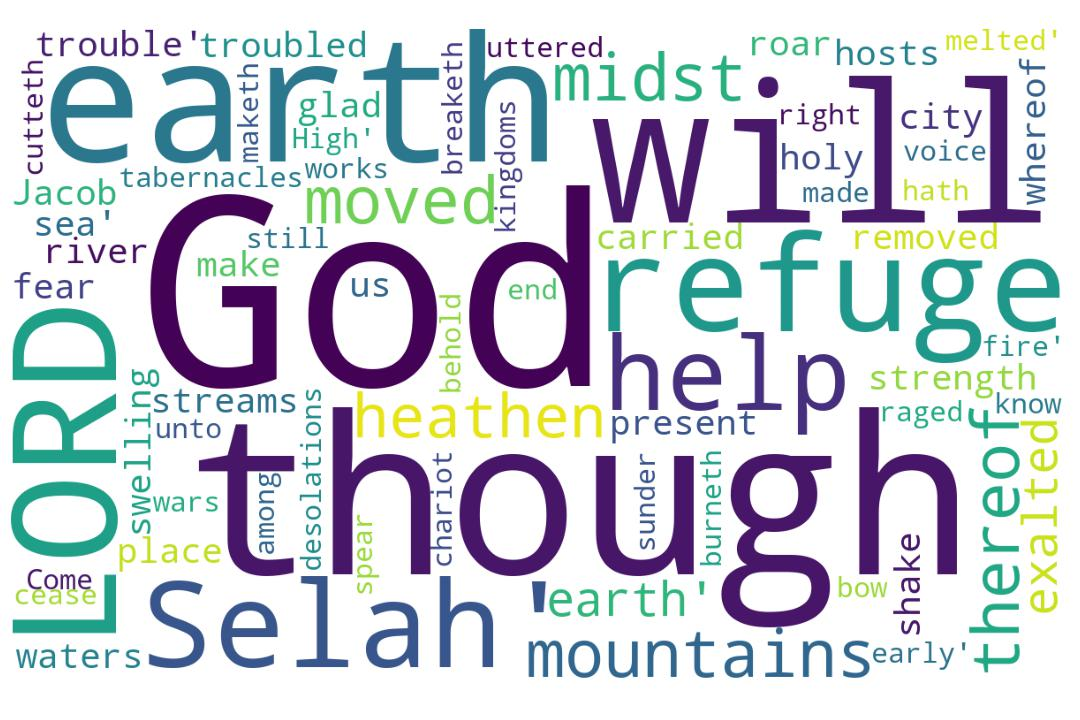
\includegraphics[width=\linewidth]{19OT-Psalms/Psalm46-WordCloud.jpg}
  \caption{Psalm 46 Word Cloud}
  \label{fig:Psalm 46 word Cloud}
\end{figure}

\marginpar{\scriptsize \centering \fcolorbox{bone}{lime}{\textbf{THERE IS A REFUGE}}\\ (Psalm 46) 
\begin{compactenum}[I.][8]
	\item There is a \textbf{Refuge} \index[scripture]{Psalms!Psa 046:01}\index[scripture]{Psalms!Psa 046:07}\index[scripture]{Psalms!Psa 046:11}(Psalm 46:1, 7, 11)
	\item There is a \textbf{Removal} of Evil \index[scripture]{Psalms!Psa 046:02}(Psa 46:2)
	\item There is a \textbf{River} of Life -- for God's People \index[scripture]{Psalms!Psa 046:04}(Psa 46:4)
	\item There is a \textbf{Raging} by God's Enemies \index[scripture]{Psalms!Psa 046:06}(Psa 46:6)
	\item There is \textbf{Ruin} for Evil \index[scripture]{Psalms!Psa 046:08}(Psa 46:8)
	\item There is a \textbf{Resolution} of the Conflict between Good and Evil \index[scripture]{Psalms!Psa 046:09}(Psa 46:9)
	\item There is a \textbf{Remedy} for Sin \index[scripture]{Psalms!Psa 046:10}(Psa 46:10)
	\item There is a \textbf{Repose} for Righteousness \index[scripture]{Psalms!Psa 046:11}(Psa 46:11)
\end{compactenum}}
    
\marginpar{\scriptsize \centering \fcolorbox{bone}{yellow}{\textbf{THERE IS A REFUGE}}\\ (Psalm 46) 
\begin{compactenum}[I.][8]
    \item \textbf{Welcome} of the Lord \index[scripture]{Psalms!Psa 046:01}\index[scripture]{Psalms!Psa 046:11} (Psa 46:1, 11)
    \item The \textbf{Water} of the Lord \index[scripture]{Psalms!Psa 046:04} (Psa 46:4)
    \item The \textbf{Words} of the Lord \index[scripture]{Psalms!Psa 046:06} (Psa 46:6)
    \item The \textbf{Works} of the Lord \index[scripture]{Psalms!Psa 046:08} (Psa 46:8)
    \item The \textbf{Wrath} of the Lord \index[scripture]{Psalms!Psa 046:09} (Psa 46:9)
    \item The \textbf{Wars} of the Lord \index[scripture]{Psalms!Psa 046:09} (Psa 46:9)
    \item The \textbf{Worship} of the Lord \index[scripture]{Psalms!Psa 046:10} (Psa 46:10)
\end{compactenum}}

\footnote{\textcolor[cmyk]{0.99998,1,0,0}{\hyperlink{TOC}{Return to end of Table of Contents.}}}\footnote{\href{https://audiobible.com/bible/psalms_46.html}{\textcolor[cmyk]{0.99998,1,0,0}{Psalms Audio}}}\textcolor[cmyk]{0.99998,1,0,0}{To the chief Musician for the sons of Korah, A Song upon Alamoth.}\\
\\
\textcolor[cmyk]{0.99998,1,0,0}{God \emph{is} our \fcolorbox{bone}{lime}{refuge} and strength, a very present help in trouble.}
[2] \textcolor[cmyk]{0.99998,1,0,0}{Therefore will not we fear, though the earth be \fcolorbox{bone}{lime}{removed}, and though the mountains be carried into the midst of the sea;}
[3] \textcolor[cmyk]{0.99998,1,0,0}{\emph{Though} the waters thereof roar \emph{and} be troubled, \emph{though} the mountains shake with the swelling thereof. Selah.}
[4] \textcolor[cmyk]{0.99998,1,0,0}{\emph{There} \emph{is} a \fcolorbox{bone}{lime}{river}, the streams whereof shall make glad the city of God, the holy \emph{place} of the tabernacles of the most High.}
[5] \textcolor[cmyk]{0.99998,1,0,0}{God \emph{is} in the midst of her; she shall not be moved: God shall help her, \emph{and} \emph{that} right early.}
[6] \textcolor[cmyk]{0.99998,1,0,0}{The heathen \fcolorbox{bone}{lime}{raged}, the kingdoms were moved: he uttered his voice, the earth melted.}\footnote{\textbf{Psalm 2:1} - Why do the heathen rage, and the people imagine a vain thing?, with \textbf{Acts 4:25} - Who by the mouth of thy servant David hast said, Why did the heathen rage, and the people imagine vain things?}\footnote{\textbf{Judges 5:5} - The mountains melted from before the LORD, even that Sinai from before the LORD God of Israel.}\footnote{\textbf{Psalm 97:5} - The hills melted like wax at the presence of the LORD, at the presence of the Lord of the whole earth.}\footnote{\textbf{Amos 9:5} - And the Lord GOD of hosts is he that toucheth the land, and it shall melt, and all that dwell therein shall mourn: and it shall rise up wholly like a flood; and shall be drowned, as by the flood of Egypt.}\footnote{\textbf{Amos 9:13} - Behold, the days come, saith the LORD, that the plowman shall overtake the reaper, and the treader of grapes him that soweth seed; and the mountains shall drop sweet wine, and all the hills shall melt.}\footnote{\textbf{Nahum 1:5} - The mountains quake at him, and the hills melt, and the earth is burned at his presence, yea, the world, and all that dwell therein.}\footnote{\textbf{2 Peter 3:10-12} - But the day of the Lord will come as a thief in the night; in the which the heavens shall pass away with a great noise, and the elements shall melt with fervent heat, the earth also and the works that are therein shall be burned up. [11] Seeing then that all these things shall be dissolved, what manner of persons ought ye to be in all holy conversation and godliness, [12] Looking for and hasting unto the coming of the day of God, wherein the heavens being on fire shall be dissolved, and the elements shall melt with fervent heat?}
[7] \textcolor[cmyk]{0.99998,1,0,0}{The LORD of hosts \emph{is} with us; the God of Jacob \emph{is} our \fcolorbox{bone}{lime}{refuge}. Selah.}
[8] \textcolor[cmyk]{0.99998,1,0,0}{Come, behold the works of the LORD, what \fcolorbox{bone}{lime}{desolations} he hath made in the earth.}\footnote{\textbf{Psalm 73:19} - How are they brought into desolation, as in a moment! they are utterly consumed with terrors.}\footnote{\textbf{Isaiah 10:3} - And what will ye do in the day of visitation, and in the desolation which shall come from far? to whom will ye flee for help? and where will ye leave your glory?}\footnote{\textbf{Isaiah 61:4} - And they shall build the old wastes, they shall raise up the former desolations, and they shall repair the waste cities, the desolations of many generations.}
[9] \textcolor[cmyk]{0.99998,1,0,0}{He maketh wars to cease unto the end of the earth; he breaketh the bow, and cutteth the spear in sunder; he burneth the chariot in the fire.}\marginpar{\scriptsize \textcolor[rgb]{0.00,0.545,0.269}{Four things the Lord does:
\begin{compactenum}
\item Maketh wars to cease
\item Breaketh the bow
\item Cutteth the spear in sunder
\item Burneth the chariot in the fire
\end{compactenum}} }\footnote{\textbf{Isaiah 2:4} - And he shall judge among the nations, and shall rebuke many people: and they shall beat their swords into plowshares, and their spears into pruninghooks: nation shall not lift up sword against nation, neither shall they learn war any more.}\footnote{\textbf{Joel 3:10} - Beat your plowshares into swords, and your pruninghooks into spears: let the weak say, I am strong.}\footnote{\textbf{Micah 4:3-7} - And he shall judge among many people, and rebuke strong nations afar off; and they shall beat their swords into plowshares, and their spears into pruninghooks: nation shall not lift up a sword against nation, neither shall they learn war any more. [4] But they shall sit every man under his vine and under his fig tree; and none shall make them afraid: for the mouth of the LORD of hosts hath spoken it. [5] For all people will walk every one in the name of his god, and we will walk in the name of the LORD our God for ever and ever. [6] In that day, saith the LORD, will I assemble her that halteth, and I will gather her that is driven out, and her that I have afflicted; [7] And I will make her that halted a remnant, and her that was cast far off a strong nation: and the LORD shall reign over them in mount Zion from henceforth, even for ever.}
[10] \textcolor[cmyk]{0.99998,1,0,0}{Be still, and know that I \emph{am} God: I will be \fcolorbox{bone}{lime}{exalted} among the heathen, I will be exalted in the earth.}
[11] \textcolor[cmyk]{0.99998,1,0,0}{The LORD of hosts \emph{is} with us; the God of Jacob \emph{is} our \fcolorbox{bone}{lime}{refuge}. Selah.}




\index[NWIV]{12!Psalms!Psa 46:1}\index[AWIP]{God!Psalms!Psa 46:1}\index[AWIP]{\emph{is}!Psalms!Psa 46:1}\index[AWIP]{our!Psalms!Psa 46:1}\index[AWIP]{refuge!Psalms!Psa 46:1}\index[AWIP]{and!Psalms!Psa 46:1}\index[AWIP]{strength!Psalms!Psa 46:1}\index[AWIP]{a!Psalms!Psa 46:1}\index[AWIP]{very!Psalms!Psa 46:1}\index[AWIP]{present!Psalms!Psa 46:1}\index[AWIP]{help!Psalms!Psa 46:1}\index[AWIP]{in!Psalms!Psa 46:1}\index[AWIP]{trouble!Psalms!Psa 46:1}\index[AWIP]{\emph{is}!Psalms!Psa 46:1}

\index[NWIV]{22!Psalms!Psa 46:2}\index[AWIP]{Therefore!Psalms!Psa 46:2}\index[AWIP]{will!Psalms!Psa 46:2}\index[AWIP]{not!Psalms!Psa 46:2}\index[AWIP]{we!Psalms!Psa 46:2}\index[AWIP]{fear!Psalms!Psa 46:2}\index[AWIP]{though!Psalms!Psa 46:2}\index[AWIP]{though!Psalms!Psa 46:2 (2)}\index[AWIP]{the!Psalms!Psa 46:2}\index[AWIP]{the!Psalms!Psa 46:2 (2)}\index[AWIP]{the!Psalms!Psa 46:2 (3)}\index[AWIP]{the!Psalms!Psa 46:2 (4)}\index[AWIP]{earth!Psalms!Psa 46:2}\index[AWIP]{be!Psalms!Psa 46:2}\index[AWIP]{be!Psalms!Psa 46:2 (2)}\index[AWIP]{removed!Psalms!Psa 46:2}\index[AWIP]{and!Psalms!Psa 46:2}\index[AWIP]{mountains!Psalms!Psa 46:2}\index[AWIP]{carried!Psalms!Psa 46:2}\index[AWIP]{into!Psalms!Psa 46:2}\index[AWIP]{midst!Psalms!Psa 46:2}\index[AWIP]{of!Psalms!Psa 46:2}\index[AWIP]{sea!Psalms!Psa 46:2}

\index[NWIV]{17!Psalms!Psa 46:3}\index[AWIP]{\emph{Though}!Psalms!Psa 46:3}\index[AWIP]{the!Psalms!Psa 46:3}\index[AWIP]{the!Psalms!Psa 46:3 (2)}\index[AWIP]{the!Psalms!Psa 46:3 (3)}\index[AWIP]{waters!Psalms!Psa 46:3}\index[AWIP]{thereof!Psalms!Psa 46:3}\index[AWIP]{thereof!Psalms!Psa 46:3 (2)}\index[AWIP]{roar!Psalms!Psa 46:3}\index[AWIP]{\emph{and}!Psalms!Psa 46:3}\index[AWIP]{be!Psalms!Psa 46:3}\index[AWIP]{troubled!Psalms!Psa 46:3}\index[AWIP]{\emph{though}!Psalms!Psa 46:3}\index[AWIP]{mountains!Psalms!Psa 46:3}\index[AWIP]{shake!Psalms!Psa 46:3}\index[AWIP]{with!Psalms!Psa 46:3}\index[AWIP]{swelling!Psalms!Psa 46:3}\index[AWIP]{Selah!Psalms!Psa 46:3}\index[AWIP]{\emph{Though}!Psalms!Psa 46:3}\index[AWIP]{\emph{and}!Psalms!Psa 46:3}\index[AWIP]{\emph{though}!Psalms!Psa 46:3}

\index[NWIV]{24!Psalms!Psa 46:4}\index[AWIP]{\emph{There}!Psalms!Psa 46:4}\index[AWIP]{\emph{is}!Psalms!Psa 46:4}\index[AWIP]{a!Psalms!Psa 46:4}\index[AWIP]{river!Psalms!Psa 46:4}\index[AWIP]{the!Psalms!Psa 46:4}\index[AWIP]{the!Psalms!Psa 46:4 (2)}\index[AWIP]{the!Psalms!Psa 46:4 (3)}\index[AWIP]{the!Psalms!Psa 46:4 (4)}\index[AWIP]{the!Psalms!Psa 46:4 (5)}\index[AWIP]{streams!Psalms!Psa 46:4}\index[AWIP]{whereof!Psalms!Psa 46:4}\index[AWIP]{shall!Psalms!Psa 46:4}\index[AWIP]{make!Psalms!Psa 46:4}\index[AWIP]{glad!Psalms!Psa 46:4}\index[AWIP]{city!Psalms!Psa 46:4}\index[AWIP]{of!Psalms!Psa 46:4}\index[AWIP]{of!Psalms!Psa 46:4 (2)}\index[AWIP]{of!Psalms!Psa 46:4 (3)}\index[AWIP]{God!Psalms!Psa 46:4}\index[AWIP]{holy!Psalms!Psa 46:4}\index[AWIP]{\emph{place}!Psalms!Psa 46:4}\index[AWIP]{tabernacles!Psalms!Psa 46:4}\index[AWIP]{most!Psalms!Psa 46:4}\index[AWIP]{High!Psalms!Psa 46:4}\index[AWIP]{\emph{There}!Psalms!Psa 46:4}\index[AWIP]{\emph{is}!Psalms!Psa 46:4}\index[AWIP]{\emph{place}!Psalms!Psa 46:4}

\index[NWIV]{20!Psalms!Psa 46:5}\index[AWIP]{God!Psalms!Psa 46:5}\index[AWIP]{God!Psalms!Psa 46:5 (2)}\index[AWIP]{\emph{is}!Psalms!Psa 46:5}\index[AWIP]{in!Psalms!Psa 46:5}\index[AWIP]{the!Psalms!Psa 46:5}\index[AWIP]{midst!Psalms!Psa 46:5}\index[AWIP]{of!Psalms!Psa 46:5}\index[AWIP]{her!Psalms!Psa 46:5}\index[AWIP]{her!Psalms!Psa 46:5 (2)}\index[AWIP]{she!Psalms!Psa 46:5}\index[AWIP]{shall!Psalms!Psa 46:5}\index[AWIP]{shall!Psalms!Psa 46:5 (2)}\index[AWIP]{not!Psalms!Psa 46:5}\index[AWIP]{be!Psalms!Psa 46:5}\index[AWIP]{moved!Psalms!Psa 46:5}\index[AWIP]{help!Psalms!Psa 46:5}\index[AWIP]{\emph{and}!Psalms!Psa 46:5}\index[AWIP]{\emph{that}!Psalms!Psa 46:5}\index[AWIP]{right!Psalms!Psa 46:5}\index[AWIP]{early!Psalms!Psa 46:5}\index[AWIP]{\emph{is}!Psalms!Psa 46:5}\index[AWIP]{\emph{and}!Psalms!Psa 46:5}\index[AWIP]{\emph{that}!Psalms!Psa 46:5}

\index[NWIV]{14!Psalms!Psa 46:6}\index[AWIP]{The!Psalms!Psa 46:6}\index[AWIP]{heathen!Psalms!Psa 46:6}\index[AWIP]{raged!Psalms!Psa 46:6}\index[AWIP]{the!Psalms!Psa 46:6}\index[AWIP]{the!Psalms!Psa 46:6 (2)}\index[AWIP]{kingdoms!Psalms!Psa 46:6}\index[AWIP]{were!Psalms!Psa 46:6}\index[AWIP]{moved!Psalms!Psa 46:6}\index[AWIP]{he!Psalms!Psa 46:6}\index[AWIP]{uttered!Psalms!Psa 46:6}\index[AWIP]{his!Psalms!Psa 46:6}\index[AWIP]{voice!Psalms!Psa 46:6}\index[AWIP]{earth!Psalms!Psa 46:6}\index[AWIP]{melted!Psalms!Psa 46:6}

\index[NWIV]{15!Psalms!Psa 46:7}\index[AWIP]{The!Psalms!Psa 46:7}\index[AWIP]{LORD!Psalms!Psa 46:7}\index[AWIP]{of!Psalms!Psa 46:7}\index[AWIP]{of!Psalms!Psa 46:7 (2)}\index[AWIP]{hosts!Psalms!Psa 46:7}\index[AWIP]{\emph{is}!Psalms!Psa 46:7}\index[AWIP]{\emph{is}!Psalms!Psa 46:7 (2)}\index[AWIP]{with!Psalms!Psa 46:7}\index[AWIP]{us!Psalms!Psa 46:7}\index[AWIP]{the!Psalms!Psa 46:7}\index[AWIP]{God!Psalms!Psa 46:7}\index[AWIP]{Jacob!Psalms!Psa 46:7}\index[AWIP]{our!Psalms!Psa 46:7}\index[AWIP]{refuge!Psalms!Psa 46:7}\index[AWIP]{Selah!Psalms!Psa 46:7}\index[AWIP]{\emph{is}!Psalms!Psa 46:7}\index[AWIP]{\emph{is}!Psalms!Psa 46:7 (2)}

\index[NWIV]{15!Psalms!Psa 46:8}\index[AWIP]{Come!Psalms!Psa 46:8}\index[AWIP]{behold!Psalms!Psa 46:8}\index[AWIP]{the!Psalms!Psa 46:8}\index[AWIP]{the!Psalms!Psa 46:8 (2)}\index[AWIP]{the!Psalms!Psa 46:8 (3)}\index[AWIP]{works!Psalms!Psa 46:8}\index[AWIP]{of!Psalms!Psa 46:8}\index[AWIP]{LORD!Psalms!Psa 46:8}\index[AWIP]{what!Psalms!Psa 46:8}\index[AWIP]{desolations!Psalms!Psa 46:8}\index[AWIP]{he!Psalms!Psa 46:8}\index[AWIP]{hath!Psalms!Psa 46:8}\index[AWIP]{made!Psalms!Psa 46:8}\index[AWIP]{in!Psalms!Psa 46:8}\index[AWIP]{earth!Psalms!Psa 46:8}

\index[NWIV]{28!Psalms!Psa 46:9}\index[AWIP]{He!Psalms!Psa 46:9}\index[AWIP]{maketh!Psalms!Psa 46:9}\index[AWIP]{wars!Psalms!Psa 46:9}\index[AWIP]{to!Psalms!Psa 46:9}\index[AWIP]{cease!Psalms!Psa 46:9}\index[AWIP]{unto!Psalms!Psa 46:9}\index[AWIP]{the!Psalms!Psa 46:9}\index[AWIP]{the!Psalms!Psa 46:9 (2)}\index[AWIP]{the!Psalms!Psa 46:9 (3)}\index[AWIP]{the!Psalms!Psa 46:9 (4)}\index[AWIP]{the!Psalms!Psa 46:9 (5)}\index[AWIP]{the!Psalms!Psa 46:9 (6)}\index[AWIP]{end!Psalms!Psa 46:9}\index[AWIP]{of!Psalms!Psa 46:9}\index[AWIP]{earth!Psalms!Psa 46:9}\index[AWIP]{he!Psalms!Psa 46:9}\index[AWIP]{he!Psalms!Psa 46:9 (2)}\index[AWIP]{breaketh!Psalms!Psa 46:9}\index[AWIP]{bow!Psalms!Psa 46:9}\index[AWIP]{and!Psalms!Psa 46:9}\index[AWIP]{cutteth!Psalms!Psa 46:9}\index[AWIP]{spear!Psalms!Psa 46:9}\index[AWIP]{in!Psalms!Psa 46:9}\index[AWIP]{in!Psalms!Psa 46:9 (2)}\index[AWIP]{sunder!Psalms!Psa 46:9}\index[AWIP]{burneth!Psalms!Psa 46:9}\index[AWIP]{chariot!Psalms!Psa 46:9}\index[AWIP]{fire!Psalms!Psa 46:9}

\index[NWIV]{22!Psalms!Psa 46:10}\index[AWIP]{Be!Psalms!Psa 46:10}\index[AWIP]{still!Psalms!Psa 46:10}\index[AWIP]{and!Psalms!Psa 46:10}\index[AWIP]{know!Psalms!Psa 46:10}\index[AWIP]{that!Psalms!Psa 46:10}\index[AWIP]{I!Psalms!Psa 46:10}\index[AWIP]{I!Psalms!Psa 46:10 (2)}\index[AWIP]{I!Psalms!Psa 46:10 (3)}\index[AWIP]{\emph{am}!Psalms!Psa 46:10}\index[AWIP]{God!Psalms!Psa 46:10}\index[AWIP]{will!Psalms!Psa 46:10}\index[AWIP]{will!Psalms!Psa 46:10 (2)}\index[AWIP]{be!Psalms!Psa 46:10}\index[AWIP]{be!Psalms!Psa 46:10 (2)}\index[AWIP]{exalted!Psalms!Psa 46:10}\index[AWIP]{exalted!Psalms!Psa 46:10 (2)}\index[AWIP]{among!Psalms!Psa 46:10}\index[AWIP]{the!Psalms!Psa 46:10}\index[AWIP]{the!Psalms!Psa 46:10 (2)}\index[AWIP]{heathen!Psalms!Psa 46:10}\index[AWIP]{in!Psalms!Psa 46:10}\index[AWIP]{earth!Psalms!Psa 46:10}\index[AWIP]{\emph{am}!Psalms!Psa 46:10}

\index[NWIV]{15!Psalms!Psa 46:11}\index[AWIP]{The!Psalms!Psa 46:11}\index[AWIP]{LORD!Psalms!Psa 46:11}\index[AWIP]{of!Psalms!Psa 46:11}\index[AWIP]{of!Psalms!Psa 46:11 (2)}\index[AWIP]{hosts!Psalms!Psa 46:11}\index[AWIP]{\emph{is}!Psalms!Psa 46:11}\index[AWIP]{\emph{is}!Psalms!Psa 46:11 (2)}\index[AWIP]{with!Psalms!Psa 46:11}\index[AWIP]{us!Psalms!Psa 46:11}\index[AWIP]{the!Psalms!Psa 46:11}\index[AWIP]{God!Psalms!Psa 46:11}\index[AWIP]{Jacob!Psalms!Psa 46:11}\index[AWIP]{our!Psalms!Psa 46:11}\index[AWIP]{refuge!Psalms!Psa 46:11}\index[AWIP]{Selah!Psalms!Psa 46:11}\index[AWIP]{\emph{is}!Psalms!Psa 46:11}\index[AWIP]{\emph{is}!Psalms!Psa 46:11 (2)}


\section{Psalm 46 Outlines}

\subsection{My Outlines}

\subsubsection{There is a Refuge}

\index[speaker]{Keith Anthony!Psalm 046 (There is a Refuge)}
\index[series]{Psalms (Keith Anthony)!Psalm 046 (There is a Refuge)}
\index[date]{2016/07/22!Psalm 046 (There is a Refuge) (Keith Anthony)}
\begin{compactenum}[I.][8]
	\item There is a \textbf{Refuge} \index[scripture]{Psalms!Psa 046:01}\index[scripture]{Psalms!Psa 046:07}\index[scripture]{Psalms!Psa 046:11}(Psa 46:1, 7, 11)
	\begin{compactenum}[A.]
		\item The Lord is described as a sure refuge throughout scripture. Proverb 14:26 states ``In the fear of the LORD is strong confidence: and his children shall have a place of refuge.''
		\item Hebrews 6:18 states ``That by two immutable things, in which it was impossible for God to lie, we might have a strong consolation, who have fled for refuge to lay hold upon the hope set before us:''
	\end{compactenum}
	\item There is a \textbf{Removal} of Evil \index[scripture]{Psalms!Psa 046:02}(Psa 46:2)
	\begin{compactenum}[A.]
		\item (Zechariah 3:9) "For behold the stone that I have laid before Joshua; upon one stone shall be seven eyes: behold, I will engrave the graving thereof, saith the LORD of hosts, and I will remove the iniquity of that land in one day."
	\end{compactenum}
	\item There is a \textbf{River} of Life -- for God's People \index[scripture]{Psalms!Psa 046:04}(Psa 46:4)
	\begin{compactenum}[A.]
		\item Revelation 22:1-2 Describes this: ``And he shewed me a pure river of water of life, clear as crystal, proceeding out of the throne of God and of the Lamb. [2] In the midst of the street of it, and on either side of the river, was there the tree of life, which bare twelve manner of fruits, and yielded her fruit every month: and the leaves of the tree were for the healing of the nations.''
	\end{compactenum}
	\item There is a \textbf{Raging} by God's Enemies \index[scripture]{Psalms!Psa 046:06}(Psa 46:6)
	\begin{compactenum}[A.]
		\item Psalm 2:1 talks of this: ``Why do the heathen rage, and the people imagine a vain thing?''
		\item Quoted in Acts 4:25: ``Who by the mouth of thy servant David hast said, Why did the heathen rage, and the people imagine vain things?''
		\item and in Nahum 2:4: ``The chariots shall rage in the streets, they shall justle one against another in the broad ways: they shall seem like torches, they shall run like the lightnings''
	\end{compactenum}
	\item There is \textbf{Ruin} for Evil \index[scripture]{Psalms!Psa 046:08}(Psa 46:8)
%	\item There is a \textbf{Resolution} of the Conflict between Good and Evil \index[scripture]{Psalms!Psa 046:09}(Psalm 46:9)
	\item There is a \textbf{Repose} for the Righteousness \index[scripture]{Psalms!Psa 046:11}(Psa 46:11)
	\begin{compactenum}[A.]
		\item Hebrews 4:9 There remaineth therefore a rest to the people of God.
	\end{compactenum}
    \item There is a \textbf{Remedy} for Sin \index[scripture]{Psalms!Psa 046:10}(Psa 46:10)
	\begin{compactenum}[A.]
		\item Ephesians 2:8 For by grace are ye saved through faith; and that not of yourselves: it is the gift of God:
	\end{compactenum}
\end{compactenum}

\subsubsection{Things of the Lord}

\index[speaker]{Keith Anthony!Psalm 046 (Things of the Lord)}
\index[series]{Psalms (Keith Anthony)!Psalm 046 (Things of the Lord)}
\index[date]{2016/07/22!Psalm 046 (Things of the Lord) (Keith Anthony)}
\begin{compactenum}[I.][8]
    \item The \textbf{Welcome} of the Lord \index[scripture]{Psalms!Psa 046:01}\index[scripture]{Psalms!Psa 046:11} (Psa 46:1, 11)
     \item The \textbf{Water} of the Lord \index[scripture]{Psalms!Psa 046:04} (Psa 46:4)
    \item The \textbf{Words} of the Lord \index[scripture]{Psalms!Psa 046:06} (Psa 46:6)
    \item The \textbf{Works} of the Lord \index[scripture]{Psalms!Psa 046:08} (Psa 46:8)
    \item The \textbf{Wrath} of the Lord \index[scripture]{Psalms!Psa 046:09} (Psa 46:9)
    \item The \textbf{Wars} of the Lord \index[scripture]{Psalms!Psa 046:09} (Psa 46:9)
    \item The \textbf{Worship} of the Lord \index[scripture]{Psalms!Psa 046:10} (Psa 46:10)
\end{compactenum}


%	\begin{compactenum}[A.]
%		\item Psalm 2:1 talks of this: ``Why do the heathen rage, and the people imagine a vain thing?''
%		\item Quoted in Acts 4:25: ``Who by the mouth of thy servant David hast said, Why did the heathen rage, and the people imagine vain things?''
%		\item and in Nahum 2:4: ``The chariots shall rage in the streets, they shall justle one against another in the broad ways: they shall seem like torches, they shall run like the lightnings''
%    \end{compactenum}

%	\begin{compactenum}[A.] There is NO remedy without the LORD
%		\item 2 Chonicles 36:16 speaks of Rebellious Israel who kept rejecting God's Pleas for them to repent: ``But they mocked the messengers of God, and despised his words, and misused his prophets, until the wrath of the LORD arose against his people, till there was no remedy.''
%	\end{compactenum}

\subsection{Outlines from Others}



\section{Psalm 46 Comments}

\subsection{Numeric Nuggets}
\textbf{13:} Verses 6, 7, 8, and 11 each contain 13 unique words.\\
\noindent \textbf{7:} The word ``God'' is used 7 times.\\
\noindent \textbf{5:} The word ``earth'' is used 5 times.



\subsection{Psalm 46:1}
One author notes that verse 1 is inscribed on the tombstone of Martin Luther.\cite{Ruckman1992PsalmsV1} What matters to a person in trouble is not past help, and not future help, but present help.
	
\subsection{Psalm 46:2}
The verse describes things that will happen at the Second Advent. All the mountains in the world will be flattened (the eventual Flat Earth that some believe in now) except for the mountain where Jerusalem sites. This place will be the highest point on Earth during the Millennium. 
	
\subsection{Psalm 46:3}
See verses like Joel 3:16 and Haggai 2:6-7 speaking of the mountains shaking.\footnote{\textbf{Joel 3:16-17} - The LORD also shall roar out of Zion, and utter his voice from Jerusalem; and the heavens and the earth shall shake: but the LORD will be the hope of his people, and the strength of the children of Israel. [17] So shall ye know that I am the LORD your God dwelling in Zion, my holy mountain: then shall Jerusalem be holy, and there shall no strangers pass through her any more.}\footnote{\textbf{Haggai 2:6-7} - For thus saith the LORD of hosts; Yet once, it is a little while, and I will shake the heavens, and the earth, and the sea, and the dry land; [7] And I will shake all nations, and the desire of all nations shall come: and I will fill this house with glory, saith the LORD of hosts.}
	
\subsection{Psalm 46:4}
This river is spoken of in Ezekiel 47. It will be in the midst of Jerusalem in the Millennium and in New Jerusalam in eternity, described in Revelation 22:1-2.\footnote{\textbf{Revelation 22:1-2} - And he shewed me a pure river of water of life, clear as crystal, proceeding out of the throne of God and of the Lamb. [2] In the midst of the street of it, and on either side of the river, was there the tree of life, which bare twelve manner of fruits, and yielded her fruit every month: and the leaves of the tree were for the healing of the nations.}

\subsection{Psalm 46:7}
Note the word ``Selah,'' which always indicates the tribulation context.  See the examples when the God of Jacob  protected Jacob:
\begin{compactenum}
	\item Protected from being killed by his brother in Genesis 27:41-46.
	\item Protected from being ignored during the blessing in Genesis 25:33-34.
	\item Protected from being cheated by Laban in Genesis 31:7.
	\item Protected from getting involved in a war over Dinah in Genesis 34:30.
	\item Protected from an early death -- lived 130 years (Genesis 47:9)
	\item Protected during the Great Tribulation, the context of Psalm 46.\cite{Ruckman1992PsalmsV1}
\end{compactenum}

\subsection{Psalm 46:8}
Compare this verse with Psalm 145:9.\footnote{\textbf{Psalm 145:9} - The LORD is good to all: and his tender mercies are over all his works.} Is this a contradiction? These works, here, involve making the Earth desolate. But they are merciful. Verse  9 explains that the Lord's ``war to end all wars'' will put an end to mankind's wars.

\subsection{Psalm 46:10}
In this age, the Lord is exalted locally, in churches where the Gospel is preached, where believers live lives to glorify him, and anyway God's truth is followed. Universally, that is worldwide, this will be true in the Millennium.

\subsection{Psalm 46 Repeated Phrases}


%%%%%%%%%%
%%%%%%%%%%
\normalsize
 
\begin{center}
\begin{longtable}{|c|c|}
\caption[Psalm 46 Repeated Phrases]{Psalm 46 Repeated Phrases}\label{table:Repeated Phrases Psalm 46} \\
\hline \multicolumn{1}{|c|}{\textbf{Phrase}} & \multicolumn{1}{c|}{\textbf{Frequency}} \\ \hline 
\endfirsthead
 
\multicolumn{2}{c}
{{\bfseries \tablename\ \thetable{} -- continued from previous page}} \\  
\hline \multicolumn{1}{|c|}{\textbf{Phrase}} & \multicolumn{1}{c|}{\textbf{Frequency}} \\ \hline 
\endhead
 
\hline \multicolumn{2}{c}{{ }} \\ \hline
\endfoot 
the earth & 5\\ \hline 
of the & 5\\ \hline 
in the & 4\\ \hline 
\emph{is} our & 3\\ \hline 
\emph{is} our refuge & 3\\ \hline 
our refuge & 3\\ \hline 
\end{longtable}
\end{center}



%%%%%%%%%%
%%%%%%%%%%



\section{Psalm 46 Statistics}

%%%%%%%%%%%%%%%%%%%%%%%%%%%
%%%%% Word Statistics
%%%%%%%%%%%%%%%%%%%%%%%%%%


\normalsize



\subsection{Chapter Word Statistics}


%%%%%%%%%%
%%%%%%%%%%
 
\begin{center}
\begin{longtable}{l|c|c|c|c}
\caption[Stats for Psalm 46]{Stats for Psalm 46} \label{table:Stats for Psalm 46} \\ 
\hline \multicolumn{1}{|c|}{\textbf{Verse(s)}} & \multicolumn{1}{|c|}{\textbf{Count}} & \multicolumn{1}{|c|}{\textbf{Unique}} & \multicolumn{1}{|c|}{\textbf{Italics}} & \multicolumn{1}{|c|}{\textbf{Uniq Italic}}  \\ \hline 
\endfirsthead
 
\multicolumn{5}{c}
{{\bfseries \tablename\ \thetable{} -- continued from previous page}} \\  
\hline \multicolumn{1}{|c|}{\textbf{Verse(s)}} & \multicolumn{1}{|c|}{\textbf{Count}} & \multicolumn{1}{|c|}{\textbf{Unique}} & \multicolumn{1}{|c|}{\textbf{Italics}} & \multicolumn{1}{|c|}{\textbf{Uniq Italic}}  \\ \hline 
\endhead
 
\hline \multicolumn{5}{|r|}{{Continued if needed}} \\ \hline
\endfoot 
1 & 12 & 12 & 1 & 1\\ \hline
2 & 22 & 17 & 0 & 0\\ \hline
3 & 17 & 14 & 3 & 3\\ \hline
4 & 24 & 18 & 3 & 3\\ \hline
5 & 20 & 17 & 3 & 3\\ \hline
6 & 14 & 13 & 0 & 0\\ \hline
7 & 15 & 13 & 2 & 1\\ \hline
8 & 15 & 13 & 0 & 0\\ \hline
9 & 28 & 21 & 0 & 0\\ \hline
10 & 22 & 16 & 1 & 1\\ \hline
11 & 15 & 13 & 2 & 1\\ \hline
\hline \hline
Total & 204 & 102 & 15 & 8



\end{longtable}
\end{center}

%%%%%%%%%%
%%%%%%%%%%
 
\subsection{Words by Frequency}

\begin{center}
\begin{longtable}{l|r}
\caption[Word Frequencies in Psalm 46]{Word Frequencies in Psalm 46} \label{table:WordsIn-Psalm-46} \\ 
\hline \multicolumn{1}{|c|}{\textbf{Word}} & \multicolumn{1}{c|}{\textbf{Frequency}} \\ \hline 
\endfirsthead
 
\multicolumn{2}{c}
{{\bfseries \tablename\ \thetable{} -- continued from previous page}} \\ 
\hline \multicolumn{1}{|c|}{\textbf{Word}} & \multicolumn{1}{c|}{\textbf{Frequency}} \\ \hline 
\endhead
 
\hline \multicolumn{2}{|r|}{{Continued if needed}} \\ \hline
\endfoot
 
\hline \hline
\endlastfoot
the & 28 \\ \hline
of & 11 \\ \hline
God & 7 \\ \hline
\emph{is} & 7 \\ \hline
in & 6 \\ \hline
be & 6 \\ \hline
earth & 5 \\ \hline
and & 4 \\ \hline
he & 4 \\ \hline
our & 3 \\ \hline
refuge & 3 \\ \hline
will & 3 \\ \hline
with & 3 \\ \hline
Selah & 3 \\ \hline
shall & 3 \\ \hline
The & 3 \\ \hline
LORD & 3 \\ \hline
I & 3 \\ \hline
a & 2 \\ \hline
help & 2 \\ \hline
not & 2 \\ \hline
though & 2 \\ \hline
mountains & 2 \\ \hline
midst & 2 \\ \hline
thereof & 2 \\ \hline
\emph{and} & 2 \\ \hline
her & 2 \\ \hline
moved & 2 \\ \hline
heathen & 2 \\ \hline
hosts & 2 \\ \hline
us & 2 \\ \hline
Jacob & 2 \\ \hline
exalted & 2 \\ \hline
strength & 1 \\ \hline
very & 1 \\ \hline
present & 1 \\ \hline
trouble & 1 \\ \hline
Therefore & 1 \\ \hline
we & 1 \\ \hline
fear & 1 \\ \hline
removed & 1 \\ \hline
carried & 1 \\ \hline
into & 1 \\ \hline
sea & 1 \\ \hline
\emph{Though} & 1 \\ \hline
waters & 1 \\ \hline
roar & 1 \\ \hline
troubled & 1 \\ \hline
\emph{though} & 1 \\ \hline
shake & 1 \\ \hline
swelling & 1 \\ \hline
\emph{There} & 1 \\ \hline
river & 1 \\ \hline
streams & 1 \\ \hline
whereof & 1 \\ \hline
make & 1 \\ \hline
glad & 1 \\ \hline
city & 1 \\ \hline
holy & 1 \\ \hline
\emph{place} & 1 \\ \hline
tabernacles & 1 \\ \hline
most & 1 \\ \hline
High & 1 \\ \hline
she & 1 \\ \hline
\emph{that} & 1 \\ \hline
right & 1 \\ \hline
early & 1 \\ \hline
raged & 1 \\ \hline
kingdoms & 1 \\ \hline
were & 1 \\ \hline
uttered & 1 \\ \hline
his & 1 \\ \hline
voice & 1 \\ \hline
melted & 1 \\ \hline
Come & 1 \\ \hline
behold & 1 \\ \hline
works & 1 \\ \hline
what & 1 \\ \hline
desolations & 1 \\ \hline
hath & 1 \\ \hline
made & 1 \\ \hline
He & 1 \\ \hline
maketh & 1 \\ \hline
wars & 1 \\ \hline
to & 1 \\ \hline
cease & 1 \\ \hline
unto & 1 \\ \hline
end & 1 \\ \hline
breaketh & 1 \\ \hline
bow & 1 \\ \hline
cutteth & 1 \\ \hline
spear & 1 \\ \hline
sunder & 1 \\ \hline
burneth & 1 \\ \hline
chariot & 1 \\ \hline
fire & 1 \\ \hline
Be & 1 \\ \hline
still & 1 \\ \hline
know & 1 \\ \hline
that & 1 \\ \hline
\emph{am} & 1 \\ \hline
among & 1 \\ \hline
\end{longtable}
\end{center}



\normalsize



\subsection{Words Alphabetically}

\begin{center}
\begin{longtable}{l|r}
\caption[Word Alphabetically in Psalm 46]{Word Alphabetically in Psalm 46} \label{table:WordsIn-Psalm-46} \\ 
\hline \multicolumn{1}{|c|}{\textbf{Word}} & \multicolumn{1}{c|}{\textbf{Frequency}} \\ \hline 
\endfirsthead
 
\multicolumn{2}{c}
{{\bfseries \tablename\ \thetable{} -- continued from previous page}} \\ 
\hline \multicolumn{1}{|c|}{\textbf{Word}} & \multicolumn{1}{c|}{\textbf{Frequency}} \\ \hline 
\endhead
 
\hline \multicolumn{2}{|r|}{{Continued if needed}} \\ \hline
\endfoot
 
\hline \hline
\endlastfoot
Be & 1 \\ \hline
Come & 1 \\ \hline
God & 7 \\ \hline
He & 1 \\ \hline
High & 1 \\ \hline
I & 3 \\ \hline
Jacob & 2 \\ \hline
LORD & 3 \\ \hline
Selah & 3 \\ \hline
The & 3 \\ \hline
Therefore & 1 \\ \hline
\emph{There} & 1 \\ \hline
\emph{Though} & 1 \\ \hline
\emph{am} & 1 \\ \hline
\emph{and} & 2 \\ \hline
\emph{is} & 7 \\ \hline
\emph{place} & 1 \\ \hline
\emph{that} & 1 \\ \hline
\emph{though} & 1 \\ \hline
a & 2 \\ \hline
among & 1 \\ \hline
and & 4 \\ \hline
be & 6 \\ \hline
behold & 1 \\ \hline
bow & 1 \\ \hline
breaketh & 1 \\ \hline
burneth & 1 \\ \hline
carried & 1 \\ \hline
cease & 1 \\ \hline
chariot & 1 \\ \hline
city & 1 \\ \hline
cutteth & 1 \\ \hline
desolations & 1 \\ \hline
early & 1 \\ \hline
earth & 5 \\ \hline
end & 1 \\ \hline
exalted & 2 \\ \hline
fear & 1 \\ \hline
fire & 1 \\ \hline
glad & 1 \\ \hline
hath & 1 \\ \hline
he & 4 \\ \hline
heathen & 2 \\ \hline
help & 2 \\ \hline
her & 2 \\ \hline
his & 1 \\ \hline
holy & 1 \\ \hline
hosts & 2 \\ \hline
in & 6 \\ \hline
into & 1 \\ \hline
kingdoms & 1 \\ \hline
know & 1 \\ \hline
made & 1 \\ \hline
make & 1 \\ \hline
maketh & 1 \\ \hline
melted & 1 \\ \hline
midst & 2 \\ \hline
most & 1 \\ \hline
mountains & 2 \\ \hline
moved & 2 \\ \hline
not & 2 \\ \hline
of & 11 \\ \hline
our & 3 \\ \hline
present & 1 \\ \hline
raged & 1 \\ \hline
refuge & 3 \\ \hline
removed & 1 \\ \hline
right & 1 \\ \hline
river & 1 \\ \hline
roar & 1 \\ \hline
sea & 1 \\ \hline
shake & 1 \\ \hline
shall & 3 \\ \hline
she & 1 \\ \hline
spear & 1 \\ \hline
still & 1 \\ \hline
streams & 1 \\ \hline
strength & 1 \\ \hline
sunder & 1 \\ \hline
swelling & 1 \\ \hline
tabernacles & 1 \\ \hline
that & 1 \\ \hline
the & 28 \\ \hline
thereof & 2 \\ \hline
though & 2 \\ \hline
to & 1 \\ \hline
trouble & 1 \\ \hline
troubled & 1 \\ \hline
unto & 1 \\ \hline
us & 2 \\ \hline
uttered & 1 \\ \hline
very & 1 \\ \hline
voice & 1 \\ \hline
wars & 1 \\ \hline
waters & 1 \\ \hline
we & 1 \\ \hline
were & 1 \\ \hline
what & 1 \\ \hline
whereof & 1 \\ \hline
will & 3 \\ \hline
with & 3 \\ \hline
works & 1 \\ \hline
\end{longtable}
\end{center}



\normalsize



\subsection{Word Lengths in Chapter}
\normalsize
\begin{longtable}{l|p{3.75in}}
\caption[Words by Length in Psalm 46]{Words by Length in Psalm 46} \label{table:WordsIn-Psalm-46} \\ 
\hline \multicolumn{1}{|c|}{\textbf{Length}} & \multicolumn{1}{c|}{\textbf{Words}} \\ \hline 
\endfirsthead
 
\multicolumn{2}{c}
{{\bfseries \tablename\ \thetable{} -- continued from previous page}} \\ 
\hline \multicolumn{1}{|c|}{\textbf{Length}} & \multicolumn{1}{c|}{\textbf{Words}} \\ \hline 
\endhead
 
\hline \multicolumn{2}{|r|}{{Continued if needed}} \\ \hline
\endfoot
 
\hline \hline
\endlastfoot
1 & a, I \\ \hline
2 & \emph{is}, in, we, be, of, he, us, He, to, Be, \emph{am} \\ \hline
3 & God, our, and, not, the, sea, \emph{and}, her, she, The, his, end, bow \\ \hline
4 & very, help, will, fear, into, roar, with, make, glad, city, holy, most, High, \emph{that}, were, LORD, Come, what, hath, made, wars, unto, fire, know, that \\ \hline
5 & earth, midst, shake, Selah, \emph{There}, river, shall, \emph{place}, moved, right, early, raged, voice, hosts, Jacob, works, cease, spear, still, among \\ \hline
6 & refuge, though, \emph{Though}, waters, \emph{though}, melted, behold, maketh, sunder \\ \hline
7 & present, trouble, removed, carried, thereof, streams, whereof, heathen, uttered, cutteth, burneth, chariot, exalted \\ \hline
8 & strength, troubled, swelling, kingdoms, breaketh \\ \hline
9 & Therefore, mountains \\ \hline
11 & tabernacles, desolations \\ \hline
\end{longtable}






%%%%%%%%%%
%%%%%%%%%%

\chapter{Proverb 15}\marginpar{\scriptsize \centering \fcolorbox{bone}{lime}{\textbf{RIGHTEOUS LIPS}}\\ (Proverbs 15:1-33) \begin{compactenum}[I.][8]
    \item \textbf{Turn Away Wrath}  \index[scripture]{Proverbs!Pro 15:01}(Pro 15:1)
    \item \textbf{Dispense Knowledge} \index[scripture]{Proverbs!Pro 15:02, 07}(Pro 15:2, 7)
    \item \textbf{Are Wholesome} \index[scripture]{Proverbs!Pro 15:04}(Pro 15:4)
    \item \textbf{Offer counsel} \index[scripture]{Proverbs!Pro 15:22}(Pro 15:22)
    \item \textbf{Speak in Due Season} \index[scripture]{Proverbs!Pro 15:23}(Pro 15:23)
    \item \textbf{Are Pure and Pleasant} \index[scripture]{Proverbs!Pro 15:26}(Pro 15:26)
    \item \textbf{Answer Slowly} \index[scripture]{Proverbs!Pro 15:28}(Pro 15:28) -- some answers are not easy
\end{compactenum}}

\marginpar{\scriptsize \centering \fcolorbox{bone}{yellow}{\textbf{RESPONDING TO CORRECTION}}\\ (Proverbs 15:1-33) \begin{compactenum}[I.][8]
    \item \textbf{Wrath}  \index[scripture]{Proverbs!Pro 15:01} 
                                      \index[scripture]{Proverbs!Pro 15:18} 
                                      (Pro 15:1, 18)
    \item \textbf{Reproof}  \index[scripture]{Proverbs!Pro 15:05} 
                                      \index[scripture]{Proverbs!Pro 15:10} 
                                      \index[scripture]{Proverbs!Pro 15:12} 
                                      \index[scripture]{Proverbs!Pro 15:31} 
                                      \index[scripture]{Proverbs!Pro 15:32}  (Pro 15:5, 10, 12, 31, 32)
    \item God's \textbf{Reconnaissance}  \index[scripture]{Proverbs!Pro 15:03}  (Pro 15:3)
    \item \textbf{Regard}  \index[scripture]{Proverbs!Pro 15:05}  (Pro 15:5)
    \item \textbf{Righteousness}  \index[scripture]{Proverbs!Pro 15:06} \index[scripture]{Proverbs!Pro 15:09} \index[scripture]{Proverbs!Pro 15:19} \index[scripture]{Proverbs!Pro 15:28} 
    \index[scripture]{Proverbs!Pro 15:29}  (Pro 15:6, 9, 19, 28, 29)
    \item \textbf{Refusal}  \index[scripture]{Proverbs!Pro 15:32}  (Pro 15:32)
    \item \textbf{Receiving}  \index[scripture]{Proverbs!Pro 15:32}  (Pro 15:32)
\end{compactenum}}
    
\footnote{\textcolor[cmyk]{0.99998,1,0,0}{\hyperlink{TOC}{Return to end of Table of Contents.}}}\footnote{\href{https://audiobible.com/bible/proverbs_15.html}{\textcolor[cmyk]{0.99998,1,0,0}{Proverbs Audio}}}\textcolor[cmyk]{0.99998,1,0,0}{A soft answer \fcolorbox{bone}{lime}{turneth away wrath}: but grievous words stir up anger.}
[2] \textcolor[cmyk]{0.99998,1,0,0}{The tongue of the wise \fcolorbox{bone}{lime}{useth knowledge} aright: but the mouth of fools poureth out foolishness.}
[3] \textcolor[cmyk]{0.99998,1,0,0}{The eyes of the LORD \emph{are} in every place, beholding the evil and the good.}
[4] \textcolor[cmyk]{0.99998,1,0,0}{\fcolorbox{bone}{lime}{A wholesome tongue} \emph{is} a tree of life: but perverseness therein \emph{is} a breach in the spirit.}
[5] \textcolor[cmyk]{0.99998,1,0,0}{A fool despiseth his father's instruction: but he \fcolorbox{bone}{bone}{that} regardeth reproof is prudent.}
[6] \textcolor[cmyk]{0.99998,1,0,0}{In the house of the righteous \emph{is} much treasure: but in the revenues of the wicked is trouble.}
[7] \textcolor[cmyk]{0.99998,1,0,0}{The lips of the wise \fcolorbox{bone}{lime}{disperse knowledge}: but the heart of the foolish \emph{doeth} not so.}
[8] \textcolor[cmyk]{0.99998,1,0,0}{The sacrifice of the wicked \emph{is} an abomination to the LORD: but the prayer of the upright \emph{is} his delight.}
[9] \textcolor[cmyk]{0.99998,1,0,0}{The way of the wicked \emph{is} an abomination unto the LORD: but he loveth him \fcolorbox{bone}{bone}{that} followeth after righteousness.}
[10] \textcolor[cmyk]{0.99998,1,0,0}{Correction \emph{is} grievous unto him \fcolorbox{bone}{bone}{that} forsaketh the way: \emph{and} he \fcolorbox{bone}{bone}{that} hateth reproof shall die.}\footnote{\textbf{Jeremiah 2:30} - In vain have I smitten your children; they received no correction: your own sword hath devoured your prophets, like a destroying lion.}\footnote{\textbf{Jeremiah 5:3} - O LORD, are not thine eyes upon the truth? thou hast stricken them, but they have not grieved; thou hast consumed them, but they have refused to receive correction: they have made their faces harder than a rock; they have refused to return.}\footnote{\textbf{Jeremiah 7:28} - But thou shalt say unto them, This is a nation that obeyeth not the voice of the LORD their God, nor receiveth correction: truth is perished, and is cut off from their mouth.}\footnote{\textbf{Zephaniah 3:2} - She obeyed not the voice; she received not correction; she trusted not in the LORD; she drew not near to her God.}\footnote{\textbf{2 Timothy 3:16} - All scripture is given by inspiration of God, and is profitable for doctrine, for reproof, for correction, for instruction in righteousness:}
[11] \textcolor[cmyk]{0.99998,1,0,0}{Hell and destruction \emph{are} before the LORD: how much more then the hearts of the children of men?}
[12] \textcolor[cmyk]{0.99998,1,0,0}{A scorner loveth not one \fcolorbox{bone}{bone}{that} reproveth him: neither will he go unto the wise.}
[13] \textcolor[cmyk]{0.99998,1,0,0}{A merry heart maketh a cheerful countenance: but by sorrow of the heart the spirit is broken.}
[14] \textcolor[cmyk]{0.99998,1,0,0}{The heart of him \fcolorbox{bone}{bone}{that} hath understanding seeketh knowledge: but the mouth of fools feedeth on foolishness.}
[15] \textcolor[cmyk]{0.99998,1,0,0}{All the days of the afflicted \emph{are} evil: but he \fcolorbox{bone}{bone}{that} is of a merry heart \emph{hath} a continual feast.}
[16] \textcolor[cmyk]{0.99998,1,0,0}{Better \emph{is} little with the fear of the LORD than great treasure and trouble therewith.}
[17] \textcolor[cmyk]{0.99998,1,0,0}{Better \emph{is} a dinner of herbs where love is, than a stalled ox and hatred therewith.}
[18] \textcolor[cmyk]{0.99998,1,0,0}{A wrathful man stirreth up strife: but \emph{he} \emph{that} \emph{is} slow to anger appeaseth strife.}
[19] \textcolor[cmyk]{0.99998,1,0,0}{The way of the slothful \emph{man} \emph{is} as an hedge of thorns: but the way of the righteous \emph{is} made plain.}
[20] \textcolor[cmyk]{0.99998,1,0,0}{A wise son maketh a glad father: but a foolish man despiseth his mother.}
[21] \textcolor[cmyk]{0.99998,1,0,0}{Folly \emph{is} joy to \emph{him} \emph{that} \emph{is} destitute of wisdom: but a man of understanding walketh uprightly.}
[22] \textcolor[cmyk]{0.99998,1,0,0}{Without \fcolorbox{bone}{lime}{counsel} purposes are disappointed: but in the multitude of \fcolorbox{bone}{lime}{counsellors} they are established.}
[23] \textcolor[cmyk]{0.99998,1,0,0}{A man hath joy by the answer of his mouth: and a word \emph{spoken} \fcolorbox{bone}{lime}{in due season}, how good \emph{is} \emph{it}!}
[24] \textcolor[cmyk]{0.99998,1,0,0}{The way of life \emph{is} above to the wise, \fcolorbox{bone}{bone}{that} he may depart from hell beneath.}
[25] \textcolor[cmyk]{0.99998,1,0,0}{The LORD will destroy the house of the proud: but he will establish the border of the widow.}
[26] \textcolor[cmyk]{0.99998,1,0,0}{The thoughts of the wicked \emph{are} an abomination to the LORD: but \emph{the} \emph{words} of the pure \emph{are} \fcolorbox{bone}{lime}{pleasant words}.}
[27] \textcolor[cmyk]{0.99998,1,0,0}{He \fcolorbox{bone}{bone}{that} is greedy of gain troubleth his own house; but he \fcolorbox{bone}{bone}{that} hateth gifts shall live.}
[28] \textcolor[cmyk]{0.99998,1,0,0}{The heart of the righteous \fcolorbox{bone}{lime}{studieth to answer}: but the mouth of the wicked poureth out evil things.}
[29] \textcolor[cmyk]{0.99998,1,0,0}{The LORD \emph{is} far from the wicked: but he heareth the prayer of the righteous.}
[30] \textcolor[cmyk]{0.99998,1,0,0}{The light of the eyes rejoiceth the heart: \emph{and} a good report maketh the bones fat.}
[31] \textcolor[cmyk]{0.99998,1,0,0}{The ear \fcolorbox{bone}{bone}{that} heareth the reproof of life abideth among the wise.}
[32] \textcolor[cmyk]{0.99998,1,0,0}{He \fcolorbox{bone}{bone}{that} refuseth instruction despiseth his own soul: but he \fcolorbox{bone}{bone}{that} heareth reproof getteth understanding.}
[33] \textcolor[cmyk]{0.99998,1,0,0}{The fear of the LORD \emph{is} the instruction of wisdom; and before honour \emph{is} humility.}



\index[NWIV]{12!Proverbs!Pro 15:1}\index[AWIP]{A!Proverbs!Pro 15:1}\index[AWIP]{soft!Proverbs!Pro 15:1}\index[AWIP]{answer!Proverbs!Pro 15:1}\index[AWIP]{turneth!Proverbs!Pro 15:1}\index[AWIP]{away!Proverbs!Pro 15:1}\index[AWIP]{wrath!Proverbs!Pro 15:1}\index[AWIP]{but!Proverbs!Pro 15:1}\index[AWIP]{grievous!Proverbs!Pro 15:1}\index[AWIP]{words!Proverbs!Pro 15:1}\index[AWIP]{stir!Proverbs!Pro 15:1}\index[AWIP]{up!Proverbs!Pro 15:1}\index[AWIP]{anger!Proverbs!Pro 15:1}

\index[NWIV]{16!Proverbs!Pro 15:2}\index[AWIP]{The!Proverbs!Pro 15:2}\index[AWIP]{tongue!Proverbs!Pro 15:2}\index[AWIP]{of!Proverbs!Pro 15:2}\index[AWIP]{of!Proverbs!Pro 15:2 (2)}\index[AWIP]{the!Proverbs!Pro 15:2}\index[AWIP]{the!Proverbs!Pro 15:2 (2)}\index[AWIP]{wise!Proverbs!Pro 15:2}\index[AWIP]{useth!Proverbs!Pro 15:2}\index[AWIP]{knowledge!Proverbs!Pro 15:2}\index[AWIP]{aright!Proverbs!Pro 15:2}\index[AWIP]{but!Proverbs!Pro 15:2}\index[AWIP]{mouth!Proverbs!Pro 15:2}\index[AWIP]{fools!Proverbs!Pro 15:2}\index[AWIP]{poureth!Proverbs!Pro 15:2}\index[AWIP]{out!Proverbs!Pro 15:2}\index[AWIP]{foolishness!Proverbs!Pro 15:2}

\index[NWIV]{15!Proverbs!Pro 15:3}\index[AWIP]{The!Proverbs!Pro 15:3}\index[AWIP]{eyes!Proverbs!Pro 15:3}\index[AWIP]{of!Proverbs!Pro 15:3}\index[AWIP]{the!Proverbs!Pro 15:3}\index[AWIP]{the!Proverbs!Pro 15:3 (2)}\index[AWIP]{the!Proverbs!Pro 15:3 (3)}\index[AWIP]{LORD!Proverbs!Pro 15:3}\index[AWIP]{\emph{are}!Proverbs!Pro 15:3}\index[AWIP]{in!Proverbs!Pro 15:3}\index[AWIP]{every!Proverbs!Pro 15:3}\index[AWIP]{place!Proverbs!Pro 15:3}\index[AWIP]{beholding!Proverbs!Pro 15:3}\index[AWIP]{evil!Proverbs!Pro 15:3}\index[AWIP]{and!Proverbs!Pro 15:3}\index[AWIP]{good!Proverbs!Pro 15:3}\index[AWIP]{\emph{are}!Proverbs!Pro 15:3}

\index[NWIV]{17!Proverbs!Pro 15:4}\index[AWIP]{A!Proverbs!Pro 15:4}\index[AWIP]{wholesome!Proverbs!Pro 15:4}\index[AWIP]{tongue!Proverbs!Pro 15:4}\index[AWIP]{\emph{is}!Proverbs!Pro 15:4}\index[AWIP]{\emph{is}!Proverbs!Pro 15:4 (2)}\index[AWIP]{a!Proverbs!Pro 15:4}\index[AWIP]{a!Proverbs!Pro 15:4 (2)}\index[AWIP]{tree!Proverbs!Pro 15:4}\index[AWIP]{of!Proverbs!Pro 15:4}\index[AWIP]{life!Proverbs!Pro 15:4}\index[AWIP]{but!Proverbs!Pro 15:4}\index[AWIP]{perverseness!Proverbs!Pro 15:4}\index[AWIP]{therein!Proverbs!Pro 15:4}\index[AWIP]{breach!Proverbs!Pro 15:4}\index[AWIP]{in!Proverbs!Pro 15:4}\index[AWIP]{the!Proverbs!Pro 15:4}\index[AWIP]{spirit!Proverbs!Pro 15:4}\index[AWIP]{\emph{is}!Proverbs!Pro 15:4}\index[AWIP]{\emph{is}!Proverbs!Pro 15:4 (2)}

\index[NWIV]{13!Proverbs!Pro 15:5}\index[AWIP]{A!Proverbs!Pro 15:5}\index[AWIP]{fool!Proverbs!Pro 15:5}\index[AWIP]{despiseth!Proverbs!Pro 15:5}\index[AWIP]{his!Proverbs!Pro 15:5}\index[AWIP]{father's!Proverbs!Pro 15:5}\index[AWIP]{instruction!Proverbs!Pro 15:5}\index[AWIP]{but!Proverbs!Pro 15:5}\index[AWIP]{he!Proverbs!Pro 15:5}\index[AWIP]{that!Proverbs!Pro 15:5}\index[AWIP]{regardeth!Proverbs!Pro 15:5}\index[AWIP]{reproof!Proverbs!Pro 15:5}\index[AWIP]{is!Proverbs!Pro 15:5}\index[AWIP]{prudent!Proverbs!Pro 15:5}

\index[NWIV]{18!Proverbs!Pro 15:6}\index[AWIP]{In!Proverbs!Pro 15:6}\index[AWIP]{the!Proverbs!Pro 15:6}\index[AWIP]{the!Proverbs!Pro 15:6 (2)}\index[AWIP]{the!Proverbs!Pro 15:6 (3)}\index[AWIP]{the!Proverbs!Pro 15:6 (4)}\index[AWIP]{house!Proverbs!Pro 15:6}\index[AWIP]{of!Proverbs!Pro 15:6}\index[AWIP]{of!Proverbs!Pro 15:6 (2)}\index[AWIP]{righteous!Proverbs!Pro 15:6}\index[AWIP]{\emph{is}!Proverbs!Pro 15:6}\index[AWIP]{much!Proverbs!Pro 15:6}\index[AWIP]{treasure!Proverbs!Pro 15:6}\index[AWIP]{but!Proverbs!Pro 15:6}\index[AWIP]{in!Proverbs!Pro 15:6}\index[AWIP]{revenues!Proverbs!Pro 15:6}\index[AWIP]{wicked!Proverbs!Pro 15:6}\index[AWIP]{is!Proverbs!Pro 15:6}\index[AWIP]{trouble!Proverbs!Pro 15:6}\index[AWIP]{\emph{is}!Proverbs!Pro 15:6}

\index[NWIV]{16!Proverbs!Pro 15:7}\index[AWIP]{The!Proverbs!Pro 15:7}\index[AWIP]{lips!Proverbs!Pro 15:7}\index[AWIP]{of!Proverbs!Pro 15:7}\index[AWIP]{of!Proverbs!Pro 15:7 (2)}\index[AWIP]{the!Proverbs!Pro 15:7}\index[AWIP]{the!Proverbs!Pro 15:7 (2)}\index[AWIP]{the!Proverbs!Pro 15:7 (3)}\index[AWIP]{wise!Proverbs!Pro 15:7}\index[AWIP]{disperse!Proverbs!Pro 15:7}\index[AWIP]{knowledge!Proverbs!Pro 15:7}\index[AWIP]{but!Proverbs!Pro 15:7}\index[AWIP]{heart!Proverbs!Pro 15:7}\index[AWIP]{foolish!Proverbs!Pro 15:7}\index[AWIP]{\emph{doeth}!Proverbs!Pro 15:7}\index[AWIP]{not!Proverbs!Pro 15:7}\index[AWIP]{so!Proverbs!Pro 15:7}\index[AWIP]{\emph{doeth}!Proverbs!Pro 15:7}

\index[NWIV]{20!Proverbs!Pro 15:8}\index[AWIP]{The!Proverbs!Pro 15:8}\index[AWIP]{sacrifice!Proverbs!Pro 15:8}\index[AWIP]{of!Proverbs!Pro 15:8}\index[AWIP]{of!Proverbs!Pro 15:8 (2)}\index[AWIP]{the!Proverbs!Pro 15:8}\index[AWIP]{the!Proverbs!Pro 15:8 (2)}\index[AWIP]{the!Proverbs!Pro 15:8 (3)}\index[AWIP]{the!Proverbs!Pro 15:8 (4)}\index[AWIP]{wicked!Proverbs!Pro 15:8}\index[AWIP]{\emph{is}!Proverbs!Pro 15:8}\index[AWIP]{\emph{is}!Proverbs!Pro 15:8 (2)}\index[AWIP]{an!Proverbs!Pro 15:8}\index[AWIP]{abomination!Proverbs!Pro 15:8}\index[AWIP]{to!Proverbs!Pro 15:8}\index[AWIP]{LORD!Proverbs!Pro 15:8}\index[AWIP]{but!Proverbs!Pro 15:8}\index[AWIP]{prayer!Proverbs!Pro 15:8}\index[AWIP]{upright!Proverbs!Pro 15:8}\index[AWIP]{his!Proverbs!Pro 15:8}\index[AWIP]{delight!Proverbs!Pro 15:8}\index[AWIP]{\emph{is}!Proverbs!Pro 15:8}\index[AWIP]{\emph{is}!Proverbs!Pro 15:8 (2)}

\index[NWIV]{19!Proverbs!Pro 15:9}\index[AWIP]{The!Proverbs!Pro 15:9}\index[AWIP]{way!Proverbs!Pro 15:9}\index[AWIP]{of!Proverbs!Pro 15:9}\index[AWIP]{the!Proverbs!Pro 15:9}\index[AWIP]{the!Proverbs!Pro 15:9 (2)}\index[AWIP]{wicked!Proverbs!Pro 15:9}\index[AWIP]{\emph{is}!Proverbs!Pro 15:9}\index[AWIP]{an!Proverbs!Pro 15:9}\index[AWIP]{abomination!Proverbs!Pro 15:9}\index[AWIP]{unto!Proverbs!Pro 15:9}\index[AWIP]{LORD!Proverbs!Pro 15:9}\index[AWIP]{but!Proverbs!Pro 15:9}\index[AWIP]{he!Proverbs!Pro 15:9}\index[AWIP]{loveth!Proverbs!Pro 15:9}\index[AWIP]{him!Proverbs!Pro 15:9}\index[AWIP]{that!Proverbs!Pro 15:9}\index[AWIP]{followeth!Proverbs!Pro 15:9}\index[AWIP]{after!Proverbs!Pro 15:9}\index[AWIP]{righteousness!Proverbs!Pro 15:9}\index[AWIP]{\emph{is}!Proverbs!Pro 15:9}

\index[NWIV]{16!Proverbs!Pro 15:10}\index[AWIP]{Correction!Proverbs!Pro 15:10}\index[AWIP]{\emph{is}!Proverbs!Pro 15:10}\index[AWIP]{grievous!Proverbs!Pro 15:10}\index[AWIP]{unto!Proverbs!Pro 15:10}\index[AWIP]{him!Proverbs!Pro 15:10}\index[AWIP]{that!Proverbs!Pro 15:10}\index[AWIP]{that!Proverbs!Pro 15:10 (2)}\index[AWIP]{forsaketh!Proverbs!Pro 15:10}\index[AWIP]{the!Proverbs!Pro 15:10}\index[AWIP]{way!Proverbs!Pro 15:10}\index[AWIP]{\emph{and}!Proverbs!Pro 15:10}\index[AWIP]{he!Proverbs!Pro 15:10}\index[AWIP]{hateth!Proverbs!Pro 15:10}\index[AWIP]{reproof!Proverbs!Pro 15:10}\index[AWIP]{shall!Proverbs!Pro 15:10}\index[AWIP]{die!Proverbs!Pro 15:10}\index[AWIP]{\emph{is}!Proverbs!Pro 15:10}\index[AWIP]{\emph{and}!Proverbs!Pro 15:10}

\index[NWIV]{18!Proverbs!Pro 15:11}\index[AWIP]{Hell!Proverbs!Pro 15:11}\index[AWIP]{and!Proverbs!Pro 15:11}\index[AWIP]{destruction!Proverbs!Pro 15:11}\index[AWIP]{\emph{are}!Proverbs!Pro 15:11}\index[AWIP]{before!Proverbs!Pro 15:11}\index[AWIP]{the!Proverbs!Pro 15:11}\index[AWIP]{the!Proverbs!Pro 15:11 (2)}\index[AWIP]{the!Proverbs!Pro 15:11 (3)}\index[AWIP]{LORD!Proverbs!Pro 15:11}\index[AWIP]{how!Proverbs!Pro 15:11}\index[AWIP]{much!Proverbs!Pro 15:11}\index[AWIP]{more!Proverbs!Pro 15:11}\index[AWIP]{then!Proverbs!Pro 15:11}\index[AWIP]{hearts!Proverbs!Pro 15:11}\index[AWIP]{of!Proverbs!Pro 15:11}\index[AWIP]{of!Proverbs!Pro 15:11 (2)}\index[AWIP]{children!Proverbs!Pro 15:11}\index[AWIP]{men?!Proverbs!Pro 15:11}\index[AWIP]{\emph{are}!Proverbs!Pro 15:11}

\index[NWIV]{15!Proverbs!Pro 15:12}\index[AWIP]{A!Proverbs!Pro 15:12}\index[AWIP]{scorner!Proverbs!Pro 15:12}\index[AWIP]{loveth!Proverbs!Pro 15:12}\index[AWIP]{not!Proverbs!Pro 15:12}\index[AWIP]{one!Proverbs!Pro 15:12}\index[AWIP]{that!Proverbs!Pro 15:12}\index[AWIP]{reproveth!Proverbs!Pro 15:12}\index[AWIP]{him!Proverbs!Pro 15:12}\index[AWIP]{neither!Proverbs!Pro 15:12}\index[AWIP]{will!Proverbs!Pro 15:12}\index[AWIP]{he!Proverbs!Pro 15:12}\index[AWIP]{go!Proverbs!Pro 15:12}\index[AWIP]{unto!Proverbs!Pro 15:12}\index[AWIP]{the!Proverbs!Pro 15:12}\index[AWIP]{wise!Proverbs!Pro 15:12}

\index[NWIV]{17!Proverbs!Pro 15:13}\index[AWIP]{A!Proverbs!Pro 15:13}\index[AWIP]{merry!Proverbs!Pro 15:13}\index[AWIP]{heart!Proverbs!Pro 15:13}\index[AWIP]{heart!Proverbs!Pro 15:13 (2)}\index[AWIP]{maketh!Proverbs!Pro 15:13}\index[AWIP]{a!Proverbs!Pro 15:13}\index[AWIP]{cheerful!Proverbs!Pro 15:13}\index[AWIP]{countenance!Proverbs!Pro 15:13}\index[AWIP]{but!Proverbs!Pro 15:13}\index[AWIP]{by!Proverbs!Pro 15:13}\index[AWIP]{sorrow!Proverbs!Pro 15:13}\index[AWIP]{of!Proverbs!Pro 15:13}\index[AWIP]{the!Proverbs!Pro 15:13}\index[AWIP]{the!Proverbs!Pro 15:13 (2)}\index[AWIP]{spirit!Proverbs!Pro 15:13}\index[AWIP]{is!Proverbs!Pro 15:13}\index[AWIP]{broken!Proverbs!Pro 15:13}

\index[NWIV]{17!Proverbs!Pro 15:14}\index[AWIP]{The!Proverbs!Pro 15:14}\index[AWIP]{heart!Proverbs!Pro 15:14}\index[AWIP]{of!Proverbs!Pro 15:14}\index[AWIP]{of!Proverbs!Pro 15:14 (2)}\index[AWIP]{him!Proverbs!Pro 15:14}\index[AWIP]{that!Proverbs!Pro 15:14}\index[AWIP]{hath!Proverbs!Pro 15:14}\index[AWIP]{understanding!Proverbs!Pro 15:14}\index[AWIP]{seeketh!Proverbs!Pro 15:14}\index[AWIP]{knowledge!Proverbs!Pro 15:14}\index[AWIP]{but!Proverbs!Pro 15:14}\index[AWIP]{the!Proverbs!Pro 15:14}\index[AWIP]{mouth!Proverbs!Pro 15:14}\index[AWIP]{fools!Proverbs!Pro 15:14}\index[AWIP]{feedeth!Proverbs!Pro 15:14}\index[AWIP]{on!Proverbs!Pro 15:14}\index[AWIP]{foolishness!Proverbs!Pro 15:14}

\index[NWIV]{20!Proverbs!Pro 15:15}\index[AWIP]{All!Proverbs!Pro 15:15}\index[AWIP]{the!Proverbs!Pro 15:15}\index[AWIP]{the!Proverbs!Pro 15:15 (2)}\index[AWIP]{days!Proverbs!Pro 15:15}\index[AWIP]{of!Proverbs!Pro 15:15}\index[AWIP]{of!Proverbs!Pro 15:15 (2)}\index[AWIP]{afflicted!Proverbs!Pro 15:15}\index[AWIP]{\emph{are}!Proverbs!Pro 15:15}\index[AWIP]{evil!Proverbs!Pro 15:15}\index[AWIP]{but!Proverbs!Pro 15:15}\index[AWIP]{he!Proverbs!Pro 15:15}\index[AWIP]{that!Proverbs!Pro 15:15}\index[AWIP]{is!Proverbs!Pro 15:15}\index[AWIP]{a!Proverbs!Pro 15:15}\index[AWIP]{a!Proverbs!Pro 15:15 (2)}\index[AWIP]{merry!Proverbs!Pro 15:15}\index[AWIP]{heart!Proverbs!Pro 15:15}\index[AWIP]{\emph{hath}!Proverbs!Pro 15:15}\index[AWIP]{continual!Proverbs!Pro 15:15}\index[AWIP]{feast!Proverbs!Pro 15:15}\index[AWIP]{\emph{are}!Proverbs!Pro 15:15}\index[AWIP]{\emph{hath}!Proverbs!Pro 15:15}

\index[NWIV]{15!Proverbs!Pro 15:16}\index[AWIP]{Better!Proverbs!Pro 15:16}\index[AWIP]{\emph{is}!Proverbs!Pro 15:16}\index[AWIP]{little!Proverbs!Pro 15:16}\index[AWIP]{with!Proverbs!Pro 15:16}\index[AWIP]{the!Proverbs!Pro 15:16}\index[AWIP]{the!Proverbs!Pro 15:16 (2)}\index[AWIP]{fear!Proverbs!Pro 15:16}\index[AWIP]{of!Proverbs!Pro 15:16}\index[AWIP]{LORD!Proverbs!Pro 15:16}\index[AWIP]{than!Proverbs!Pro 15:16}\index[AWIP]{great!Proverbs!Pro 15:16}\index[AWIP]{treasure!Proverbs!Pro 15:16}\index[AWIP]{and!Proverbs!Pro 15:16}\index[AWIP]{trouble!Proverbs!Pro 15:16}\index[AWIP]{therewith!Proverbs!Pro 15:16}\index[AWIP]{\emph{is}!Proverbs!Pro 15:16}

\index[NWIV]{16!Proverbs!Pro 15:17}\index[AWIP]{Better!Proverbs!Pro 15:17}\index[AWIP]{\emph{is}!Proverbs!Pro 15:17}\index[AWIP]{a!Proverbs!Pro 15:17}\index[AWIP]{a!Proverbs!Pro 15:17 (2)}\index[AWIP]{dinner!Proverbs!Pro 15:17}\index[AWIP]{of!Proverbs!Pro 15:17}\index[AWIP]{herbs!Proverbs!Pro 15:17}\index[AWIP]{where!Proverbs!Pro 15:17}\index[AWIP]{love!Proverbs!Pro 15:17}\index[AWIP]{is!Proverbs!Pro 15:17}\index[AWIP]{than!Proverbs!Pro 15:17}\index[AWIP]{stalled!Proverbs!Pro 15:17}\index[AWIP]{ox!Proverbs!Pro 15:17}\index[AWIP]{and!Proverbs!Pro 15:17}\index[AWIP]{hatred!Proverbs!Pro 15:17}\index[AWIP]{therewith!Proverbs!Pro 15:17}\index[AWIP]{\emph{is}!Proverbs!Pro 15:17}

\index[NWIV]{15!Proverbs!Pro 15:18}\index[AWIP]{A!Proverbs!Pro 15:18}\index[AWIP]{wrathful!Proverbs!Pro 15:18}\index[AWIP]{man!Proverbs!Pro 15:18}\index[AWIP]{stirreth!Proverbs!Pro 15:18}\index[AWIP]{up!Proverbs!Pro 15:18}\index[AWIP]{strife!Proverbs!Pro 15:18}\index[AWIP]{strife!Proverbs!Pro 15:18 (2)}\index[AWIP]{but!Proverbs!Pro 15:18}\index[AWIP]{\emph{he}!Proverbs!Pro 15:18}\index[AWIP]{\emph{that}!Proverbs!Pro 15:18}\index[AWIP]{\emph{is}!Proverbs!Pro 15:18}\index[AWIP]{slow!Proverbs!Pro 15:18}\index[AWIP]{to!Proverbs!Pro 15:18}\index[AWIP]{anger!Proverbs!Pro 15:18}\index[AWIP]{appeaseth!Proverbs!Pro 15:18}\index[AWIP]{\emph{he}!Proverbs!Pro 15:18}\index[AWIP]{\emph{that}!Proverbs!Pro 15:18}\index[AWIP]{\emph{is}!Proverbs!Pro 15:18}

\index[NWIV]{21!Proverbs!Pro 15:19}\index[AWIP]{The!Proverbs!Pro 15:19}\index[AWIP]{way!Proverbs!Pro 15:19}\index[AWIP]{way!Proverbs!Pro 15:19 (2)}\index[AWIP]{of!Proverbs!Pro 15:19}\index[AWIP]{of!Proverbs!Pro 15:19 (2)}\index[AWIP]{of!Proverbs!Pro 15:19 (3)}\index[AWIP]{the!Proverbs!Pro 15:19}\index[AWIP]{the!Proverbs!Pro 15:19 (2)}\index[AWIP]{the!Proverbs!Pro 15:19 (3)}\index[AWIP]{slothful!Proverbs!Pro 15:19}\index[AWIP]{\emph{man}!Proverbs!Pro 15:19}\index[AWIP]{\emph{is}!Proverbs!Pro 15:19}\index[AWIP]{\emph{is}!Proverbs!Pro 15:19 (2)}\index[AWIP]{as!Proverbs!Pro 15:19}\index[AWIP]{an!Proverbs!Pro 15:19}\index[AWIP]{hedge!Proverbs!Pro 15:19}\index[AWIP]{thorns!Proverbs!Pro 15:19}\index[AWIP]{but!Proverbs!Pro 15:19}\index[AWIP]{righteous!Proverbs!Pro 15:19}\index[AWIP]{made!Proverbs!Pro 15:19}\index[AWIP]{plain!Proverbs!Pro 15:19}\index[AWIP]{\emph{man}!Proverbs!Pro 15:19}\index[AWIP]{\emph{is}!Proverbs!Pro 15:19}\index[AWIP]{\emph{is}!Proverbs!Pro 15:19 (2)}

\index[NWIV]{14!Proverbs!Pro 15:20}\index[AWIP]{A!Proverbs!Pro 15:20}\index[AWIP]{wise!Proverbs!Pro 15:20}\index[AWIP]{son!Proverbs!Pro 15:20}\index[AWIP]{maketh!Proverbs!Pro 15:20}\index[AWIP]{a!Proverbs!Pro 15:20}\index[AWIP]{a!Proverbs!Pro 15:20 (2)}\index[AWIP]{glad!Proverbs!Pro 15:20}\index[AWIP]{father!Proverbs!Pro 15:20}\index[AWIP]{but!Proverbs!Pro 15:20}\index[AWIP]{foolish!Proverbs!Pro 15:20}\index[AWIP]{man!Proverbs!Pro 15:20}\index[AWIP]{despiseth!Proverbs!Pro 15:20}\index[AWIP]{his!Proverbs!Pro 15:20}\index[AWIP]{mother!Proverbs!Pro 15:20}

\index[NWIV]{17!Proverbs!Pro 15:21}\index[AWIP]{Folly!Proverbs!Pro 15:21}\index[AWIP]{\emph{is}!Proverbs!Pro 15:21}\index[AWIP]{\emph{is}!Proverbs!Pro 15:21 (2)}\index[AWIP]{joy!Proverbs!Pro 15:21}\index[AWIP]{to!Proverbs!Pro 15:21}\index[AWIP]{\emph{him}!Proverbs!Pro 15:21}\index[AWIP]{\emph{that}!Proverbs!Pro 15:21}\index[AWIP]{destitute!Proverbs!Pro 15:21}\index[AWIP]{of!Proverbs!Pro 15:21}\index[AWIP]{of!Proverbs!Pro 15:21 (2)}\index[AWIP]{wisdom!Proverbs!Pro 15:21}\index[AWIP]{but!Proverbs!Pro 15:21}\index[AWIP]{a!Proverbs!Pro 15:21}\index[AWIP]{man!Proverbs!Pro 15:21}\index[AWIP]{understanding!Proverbs!Pro 15:21}\index[AWIP]{walketh!Proverbs!Pro 15:21}\index[AWIP]{uprightly!Proverbs!Pro 15:21}\index[AWIP]{\emph{is}!Proverbs!Pro 15:21}\index[AWIP]{\emph{is}!Proverbs!Pro 15:21 (2)}\index[AWIP]{\emph{him}!Proverbs!Pro 15:21}\index[AWIP]{\emph{that}!Proverbs!Pro 15:21}

\index[NWIV]{14!Proverbs!Pro 15:22}\index[AWIP]{Without!Proverbs!Pro 15:22}\index[AWIP]{counsel!Proverbs!Pro 15:22}\index[AWIP]{purposes!Proverbs!Pro 15:22}\index[AWIP]{are!Proverbs!Pro 15:22}\index[AWIP]{are!Proverbs!Pro 15:22 (2)}\index[AWIP]{disappointed!Proverbs!Pro 15:22}\index[AWIP]{but!Proverbs!Pro 15:22}\index[AWIP]{in!Proverbs!Pro 15:22}\index[AWIP]{the!Proverbs!Pro 15:22}\index[AWIP]{multitude!Proverbs!Pro 15:22}\index[AWIP]{of!Proverbs!Pro 15:22}\index[AWIP]{counsellors!Proverbs!Pro 15:22}\index[AWIP]{they!Proverbs!Pro 15:22}\index[AWIP]{established!Proverbs!Pro 15:22}

\index[NWIV]{21!Proverbs!Pro 15:23}\index[AWIP]{A!Proverbs!Pro 15:23}\index[AWIP]{man!Proverbs!Pro 15:23}\index[AWIP]{hath!Proverbs!Pro 15:23}\index[AWIP]{joy!Proverbs!Pro 15:23}\index[AWIP]{by!Proverbs!Pro 15:23}\index[AWIP]{the!Proverbs!Pro 15:23}\index[AWIP]{answer!Proverbs!Pro 15:23}\index[AWIP]{of!Proverbs!Pro 15:23}\index[AWIP]{his!Proverbs!Pro 15:23}\index[AWIP]{mouth!Proverbs!Pro 15:23}\index[AWIP]{and!Proverbs!Pro 15:23}\index[AWIP]{a!Proverbs!Pro 15:23}\index[AWIP]{word!Proverbs!Pro 15:23}\index[AWIP]{\emph{spoken}!Proverbs!Pro 15:23}\index[AWIP]{in!Proverbs!Pro 15:23}\index[AWIP]{due!Proverbs!Pro 15:23}\index[AWIP]{season!Proverbs!Pro 15:23}\index[AWIP]{how!Proverbs!Pro 15:23}\index[AWIP]{good!Proverbs!Pro 15:23}\index[AWIP]{\emph{is}!Proverbs!Pro 15:23}\index[AWIP]{\emph{it}!!Proverbs!Pro 15:23}\index[AWIP]{\emph{spoken}!Proverbs!Pro 15:23}\index[AWIP]{\emph{is}!Proverbs!Pro 15:23}\index[AWIP]{\emph{it}!!Proverbs!Pro 15:23}

\index[NWIV]{16!Proverbs!Pro 15:24}\index[AWIP]{The!Proverbs!Pro 15:24}\index[AWIP]{way!Proverbs!Pro 15:24}\index[AWIP]{of!Proverbs!Pro 15:24}\index[AWIP]{life!Proverbs!Pro 15:24}\index[AWIP]{\emph{is}!Proverbs!Pro 15:24}\index[AWIP]{above!Proverbs!Pro 15:24}\index[AWIP]{to!Proverbs!Pro 15:24}\index[AWIP]{the!Proverbs!Pro 15:24}\index[AWIP]{wise!Proverbs!Pro 15:24}\index[AWIP]{that!Proverbs!Pro 15:24}\index[AWIP]{he!Proverbs!Pro 15:24}\index[AWIP]{may!Proverbs!Pro 15:24}\index[AWIP]{depart!Proverbs!Pro 15:24}\index[AWIP]{from!Proverbs!Pro 15:24}\index[AWIP]{hell!Proverbs!Pro 15:24}\index[AWIP]{beneath!Proverbs!Pro 15:24}\index[AWIP]{\emph{is}!Proverbs!Pro 15:24}

\index[NWIV]{18!Proverbs!Pro 15:25}\index[AWIP]{The!Proverbs!Pro 15:25}\index[AWIP]{LORD!Proverbs!Pro 15:25}\index[AWIP]{will!Proverbs!Pro 15:25}\index[AWIP]{will!Proverbs!Pro 15:25 (2)}\index[AWIP]{destroy!Proverbs!Pro 15:25}\index[AWIP]{the!Proverbs!Pro 15:25}\index[AWIP]{the!Proverbs!Pro 15:25 (2)}\index[AWIP]{the!Proverbs!Pro 15:25 (3)}\index[AWIP]{the!Proverbs!Pro 15:25 (4)}\index[AWIP]{house!Proverbs!Pro 15:25}\index[AWIP]{of!Proverbs!Pro 15:25}\index[AWIP]{of!Proverbs!Pro 15:25 (2)}\index[AWIP]{proud!Proverbs!Pro 15:25}\index[AWIP]{but!Proverbs!Pro 15:25}\index[AWIP]{he!Proverbs!Pro 15:25}\index[AWIP]{establish!Proverbs!Pro 15:25}\index[AWIP]{border!Proverbs!Pro 15:25}\index[AWIP]{widow!Proverbs!Pro 15:25}

\index[NWIV]{20!Proverbs!Pro 15:26}\index[AWIP]{The!Proverbs!Pro 15:26}\index[AWIP]{thoughts!Proverbs!Pro 15:26}\index[AWIP]{of!Proverbs!Pro 15:26}\index[AWIP]{of!Proverbs!Pro 15:26 (2)}\index[AWIP]{the!Proverbs!Pro 15:26}\index[AWIP]{the!Proverbs!Pro 15:26 (2)}\index[AWIP]{the!Proverbs!Pro 15:26 (3)}\index[AWIP]{wicked!Proverbs!Pro 15:26}\index[AWIP]{\emph{are}!Proverbs!Pro 15:26}\index[AWIP]{\emph{are}!Proverbs!Pro 15:26 (2)}\index[AWIP]{an!Proverbs!Pro 15:26}\index[AWIP]{abomination!Proverbs!Pro 15:26}\index[AWIP]{to!Proverbs!Pro 15:26}\index[AWIP]{LORD!Proverbs!Pro 15:26}\index[AWIP]{but!Proverbs!Pro 15:26}\index[AWIP]{\emph{the}!Proverbs!Pro 15:26}\index[AWIP]{\emph{words}!Proverbs!Pro 15:26}\index[AWIP]{pure!Proverbs!Pro 15:26}\index[AWIP]{pleasant!Proverbs!Pro 15:26}\index[AWIP]{words!Proverbs!Pro 15:26}\index[AWIP]{\emph{are}!Proverbs!Pro 15:26}\index[AWIP]{\emph{are}!Proverbs!Pro 15:26 (2)}\index[AWIP]{\emph{the}!Proverbs!Pro 15:26}\index[AWIP]{\emph{words}!Proverbs!Pro 15:26}

\index[NWIV]{17!Proverbs!Pro 15:27}\index[AWIP]{He!Proverbs!Pro 15:27}\index[AWIP]{that!Proverbs!Pro 15:27}\index[AWIP]{that!Proverbs!Pro 15:27 (2)}\index[AWIP]{is!Proverbs!Pro 15:27}\index[AWIP]{greedy!Proverbs!Pro 15:27}\index[AWIP]{of!Proverbs!Pro 15:27}\index[AWIP]{gain!Proverbs!Pro 15:27}\index[AWIP]{troubleth!Proverbs!Pro 15:27}\index[AWIP]{his!Proverbs!Pro 15:27}\index[AWIP]{own!Proverbs!Pro 15:27}\index[AWIP]{house!Proverbs!Pro 15:27}\index[AWIP]{but!Proverbs!Pro 15:27}\index[AWIP]{he!Proverbs!Pro 15:27}\index[AWIP]{hateth!Proverbs!Pro 15:27}\index[AWIP]{gifts!Proverbs!Pro 15:27}\index[AWIP]{shall!Proverbs!Pro 15:27}\index[AWIP]{live!Proverbs!Pro 15:27}

\index[NWIV]{18!Proverbs!Pro 15:28}\index[AWIP]{The!Proverbs!Pro 15:28}\index[AWIP]{heart!Proverbs!Pro 15:28}\index[AWIP]{of!Proverbs!Pro 15:28}\index[AWIP]{of!Proverbs!Pro 15:28 (2)}\index[AWIP]{the!Proverbs!Pro 15:28}\index[AWIP]{the!Proverbs!Pro 15:28 (2)}\index[AWIP]{the!Proverbs!Pro 15:28 (3)}\index[AWIP]{righteous!Proverbs!Pro 15:28}\index[AWIP]{studieth!Proverbs!Pro 15:28}\index[AWIP]{to!Proverbs!Pro 15:28}\index[AWIP]{answer!Proverbs!Pro 15:28}\index[AWIP]{but!Proverbs!Pro 15:28}\index[AWIP]{mouth!Proverbs!Pro 15:28}\index[AWIP]{wicked!Proverbs!Pro 15:28}\index[AWIP]{poureth!Proverbs!Pro 15:28}\index[AWIP]{out!Proverbs!Pro 15:28}\index[AWIP]{evil!Proverbs!Pro 15:28}\index[AWIP]{things!Proverbs!Pro 15:28}

\index[NWIV]{15!Proverbs!Pro 15:29}\index[AWIP]{The!Proverbs!Pro 15:29}\index[AWIP]{LORD!Proverbs!Pro 15:29}\index[AWIP]{\emph{is}!Proverbs!Pro 15:29}\index[AWIP]{far!Proverbs!Pro 15:29}\index[AWIP]{from!Proverbs!Pro 15:29}\index[AWIP]{the!Proverbs!Pro 15:29}\index[AWIP]{the!Proverbs!Pro 15:29 (2)}\index[AWIP]{the!Proverbs!Pro 15:29 (3)}\index[AWIP]{wicked!Proverbs!Pro 15:29}\index[AWIP]{but!Proverbs!Pro 15:29}\index[AWIP]{he!Proverbs!Pro 15:29}\index[AWIP]{heareth!Proverbs!Pro 15:29}\index[AWIP]{prayer!Proverbs!Pro 15:29}\index[AWIP]{of!Proverbs!Pro 15:29}\index[AWIP]{righteous!Proverbs!Pro 15:29}\index[AWIP]{\emph{is}!Proverbs!Pro 15:29}

\index[NWIV]{16!Proverbs!Pro 15:30}\index[AWIP]{The!Proverbs!Pro 15:30}\index[AWIP]{light!Proverbs!Pro 15:30}\index[AWIP]{of!Proverbs!Pro 15:30}\index[AWIP]{the!Proverbs!Pro 15:30}\index[AWIP]{the!Proverbs!Pro 15:30 (2)}\index[AWIP]{the!Proverbs!Pro 15:30 (3)}\index[AWIP]{eyes!Proverbs!Pro 15:30}\index[AWIP]{rejoiceth!Proverbs!Pro 15:30}\index[AWIP]{heart!Proverbs!Pro 15:30}\index[AWIP]{\emph{and}!Proverbs!Pro 15:30}\index[AWIP]{a!Proverbs!Pro 15:30}\index[AWIP]{good!Proverbs!Pro 15:30}\index[AWIP]{report!Proverbs!Pro 15:30}\index[AWIP]{maketh!Proverbs!Pro 15:30}\index[AWIP]{bones!Proverbs!Pro 15:30}\index[AWIP]{fat!Proverbs!Pro 15:30}\index[AWIP]{\emph{and}!Proverbs!Pro 15:30}

\index[NWIV]{12!Proverbs!Pro 15:31}\index[AWIP]{The!Proverbs!Pro 15:31}\index[AWIP]{ear!Proverbs!Pro 15:31}\index[AWIP]{that!Proverbs!Pro 15:31}\index[AWIP]{heareth!Proverbs!Pro 15:31}\index[AWIP]{the!Proverbs!Pro 15:31}\index[AWIP]{the!Proverbs!Pro 15:31 (2)}\index[AWIP]{reproof!Proverbs!Pro 15:31}\index[AWIP]{of!Proverbs!Pro 15:31}\index[AWIP]{life!Proverbs!Pro 15:31}\index[AWIP]{abideth!Proverbs!Pro 15:31}\index[AWIP]{among!Proverbs!Pro 15:31}\index[AWIP]{wise!Proverbs!Pro 15:31}

\index[NWIV]{15!Proverbs!Pro 15:32}\index[AWIP]{He!Proverbs!Pro 15:32}\index[AWIP]{that!Proverbs!Pro 15:32}\index[AWIP]{that!Proverbs!Pro 15:32 (2)}\index[AWIP]{refuseth!Proverbs!Pro 15:32}\index[AWIP]{instruction!Proverbs!Pro 15:32}\index[AWIP]{despiseth!Proverbs!Pro 15:32}\index[AWIP]{his!Proverbs!Pro 15:32}\index[AWIP]{own!Proverbs!Pro 15:32}\index[AWIP]{soul!Proverbs!Pro 15:32}\index[AWIP]{but!Proverbs!Pro 15:32}\index[AWIP]{he!Proverbs!Pro 15:32}\index[AWIP]{heareth!Proverbs!Pro 15:32}\index[AWIP]{reproof!Proverbs!Pro 15:32}\index[AWIP]{getteth!Proverbs!Pro 15:32}\index[AWIP]{understanding!Proverbs!Pro 15:32}

\index[NWIV]{15!Proverbs!Pro 15:33}\index[AWIP]{The!Proverbs!Pro 15:33}\index[AWIP]{fear!Proverbs!Pro 15:33}\index[AWIP]{of!Proverbs!Pro 15:33}\index[AWIP]{of!Proverbs!Pro 15:33 (2)}\index[AWIP]{the!Proverbs!Pro 15:33}\index[AWIP]{the!Proverbs!Pro 15:33 (2)}\index[AWIP]{LORD!Proverbs!Pro 15:33}\index[AWIP]{\emph{is}!Proverbs!Pro 15:33}\index[AWIP]{\emph{is}!Proverbs!Pro 15:33 (2)}\index[AWIP]{instruction!Proverbs!Pro 15:33}\index[AWIP]{wisdom!Proverbs!Pro 15:33}\index[AWIP]{and!Proverbs!Pro 15:33}\index[AWIP]{before!Proverbs!Pro 15:33}\index[AWIP]{honour!Proverbs!Pro 15:33}\index[AWIP]{humility!Proverbs!Pro 15:33}\index[AWIP]{\emph{is}!Proverbs!Pro 15:33}\index[AWIP]{\emph{is}!Proverbs!Pro 15:33 (2)}

%%%%%%%%%%%%%%%%%%%%%%%%%%%%%%%%%%%%%%%%%%


\index[DOCTRINES]{Practicology - Seeking!Proverbs!Pro 15:14}

\index[DOCTRINES]{Practicology - Speech!Proverbs!Pro 15:01}
\index[DOCTRINES]{Practicology - Speech!Proverbs!Pro 15:02}
\index[DOCTRINES]{Practicology - Speech!Proverbs!Pro 15:04}
\index[DOCTRINES]{Practicology - Speech!Proverbs!Pro 15:07}
\index[DOCTRINES]{Practicology - Speech!Proverbs!Pro 15:23}
\index[DOCTRINES]{Practicology - Speech!Proverbs!Pro 15:28}
\index[DOCTRINES]{Practicology - Speech!Proverbs!Pro 15:29}


\index[DOCTRINES]{Practicology - Strife!Proverbs!Pro 15:18}


\index[DOCTRINES]{Practicology - Substance!Proverbs!Pro 15:06}

\index[DOCTRINES]{Practicology - Superiority!Proverbs!Pro 15:24}

\index[DOCTRINES]{Practicology - Suppication!Proverbs!Pro 15:08}



\section{Proverbs 15 Outlines}

\subsection{My Outlines}

\subsubsection{Righteous Lips}

\index[speaker]{Keith Anthony!Proverb 15 (Righteous Lips)}
\index[series]{Proverbs (Keith Anthony)!Pro 15 (Righteous Lips)}
\index[date]{2016/05/15!Proverb 15 (Righteous Lips) (Keith Anthony)}
\textbf{Introduction: } (cf Prov 16:13)
\begin{compactenum}[I.]
    \item \textbf{Turn Away Wrath}  \index[scripture]{Proverbs!Pro 15:01}(Pro 15:1)
    \item \textbf{Dispense Knowledge} \index[scripture]{Proverbs!Pro 15:02, 07}(Pro 15:2, 7)
    \item \textbf{Are Wholesome} \index[scripture]{Proverbs!Pro 15:04}(Pro 15:4)
    \item \textbf{Offer counsel} \index[scripture]{Proverbs!Pro 15:22}(Pro 15:22)
    \item \textbf{Speak in Due Season} \index[scripture]{Proverbs!Pro 15:23}(Pro 15:23)
    \item \textbf{Are Pure and Pleasant} \index[scripture]{Proverbs!Pro 15:26}(Pro 15:26)
    \item \textbf{Answer Slowly} \index[scripture]{Proverbs!Pro 15:28}(Pro 15:28) -- because some answers are not easy answers
\end{compactenum}

\subsubsection{Responding to Correction}

\index[speaker]{Keith Anthony!Proverb 15 (Responding to Correction)}
\index[series]{Proverbs (Keith Anthony)!Pro 15 (Responding to Correction)}
\index[date]{2016/05/15!Proverb 15 (Responding to Correction) (Keith Anthony)}


\begin{compactenum}[I.][8]
    \item \textbf{Wrath}  \index[scripture]{Proverbs!Pro 15:01} 
                                      \index[scripture]{Proverbs!Pro 15:18} 
                                      (Pro 15:1, 18)
    \item \textbf{Reproof}  \index[scripture]{Proverbs!Pro 15:05} 
                                      \index[scripture]{Proverbs!Pro 15:10} 
                                      \index[scripture]{Proverbs!Pro 15:12} 
                                      \index[scripture]{Proverbs!Pro 15:31} 
                                      \index[scripture]{Proverbs!Pro 15:32}  (Pro 15:5, 10, 12, 31, 32)
    \item God's \textbf{Reconnaissance}  \index[scripture]{Proverbs!Pro 15:03}  (Pro 15:3)
    \item \textbf{Regard}  \index[scripture]{Proverbs!Pro 15:05}  (Pro 15:5)
    \item \textbf{Righteousness}  \index[scripture]{Proverbs!Pro 15:06} 
                                      \index[scripture]{Proverbs!Pro 15:09} 
                                      \index[scripture]{Proverbs!Pro 15:19} 
                                      \index[scripture]{Proverbs!Pro 15:28} 
                                      \index[scripture]{Proverbs!Pro 15:29}  (Pro 15:6, 9, 19, 28, 29)
    \item \textbf{Refusal}  \index[scripture]{Proverbs!Pro 15:32}  (Pro 15:32)
    \item \textbf{Receiving}  \index[scripture]{Proverbs!Pro 15:32}  (Pro 15:32)
\end{compactenum}

\subsection{Outlines from Others}


\section{Proverb 15 Comments}

\subsection{Numeric Nuggets}
\textbf{13:} Verse 5 has 13 words. Verses 3, 5, 7, 20, 22, 25, and 29 have 13 unique words. There  are 13 total unique italic words in the chapter. The word ``that'' is used 13 times in the chapter. 

\subsection{Proverb 15:32}
The word ``reproof'' is used 13 times in the book of Proverbs, indicating man's response: (1) Prov 1:23 - \textbf{turning at reproof}, (2) Prov 1:25 - \textbf{rejecting reproof}, (3) Prov 1:30, Prov 12:1, and Prov 15:10 - \textbf{hating reproof}, (4) Prov 5:12 - \textbf{despising reproof}, (5) Prov 10:17 - \textbf{Refusing reproof}, (6) Prov 13:18 and Prov 15:5 - \textbf{regarding reproof}, (7) Prov 15:31 and Prov 15:32 - \textbf{hearing reproof}, (8) Prov 18:10 - \textbf{reproof has entry into a wise man's life}, and (9) Prov 29:15 - \textbf{reproof gives wisdom.}
\subsection{Proverb 15 Repeated Phrases}


%%%%%%%%%%
%%%%%%%%%%
\normalsize
 
\begin{center}
\begin{longtable}{|c|c|}
\caption[Proverb 15 Repeated Phrases]{Proverb 15 Repeated Phrases}\label{table:Repeated Phrases Proverb 15} \\
\hline \multicolumn{1}{|c|}{\textbf{Phrase}} & \multicolumn{1}{c|}{\textbf{Frequency}} \\ \hline 
\endfirsthead
 
\multicolumn{2}{c}
{{\bfseries \tablename\ \thetable{} -- continued from previous page}} \\  
\hline \multicolumn{1}{|c|}{\textbf{Phrase}} & \multicolumn{1}{c|}{\textbf{Frequency}} \\ \hline 
\endhead
 
\hline \multicolumn{2}{c}{{ }} \\ \hline
\endfoot 
of the & 24\\ \hline 
the LORD & 7\\ \hline 
but he & 7\\ \hline 
but the & 6\\ \hline 
the wicked & 6\\ \hline 
the wise & 5\\ \hline 
he that & 5\\ \hline 
of the wicked & 5\\ \hline 
but he that & 4\\ \hline 
of the righteous & 4\\ \hline 
the righteous & 4\\ \hline 
way of & 4\\ \hline 
but the mouth & 3\\ \hline 
but the mouth of & 3\\ \hline 
the mouth & 3\\ \hline 
the mouth of & 3\\ \hline 
mouth of & 3\\ \hline 
of the LORD & 3\\ \hline 
\emph{is} a & 3\\ \hline 
of life & 3\\ \hline 
in the & 3\\ \hline 
despiseth his & 3\\ \hline 
the heart & 3\\ \hline 
heart of & 3\\ \hline 
an abomination & 3\\ \hline 
to the & 3\\ \hline 
the LORD but & 3\\ \hline 
LORD but & 3\\ \hline 
The way & 3\\ \hline 
The way of & 3\\ \hline 
way of the & 3\\ \hline 
him that & 3\\ \hline 
\end{longtable}
\end{center}



%%%%%%%%%%
%%%%%%%%%%



%\newpage
\section{Proverb 15 Statistics}

%%%%%%%%%%%%%%%%%%%%%%%%%%%
%%%%% Word Statistics
%%%%%%%%%%%%%%%%%%%%%%%%%%

\normalsize
\subsection{Chapter Word Statistics}


%%%%%%%%%%
%%%%%%%%%%
 
\begin{center}
\begin{longtable}{l|c|c|c|c}
\caption[Stats for Proverb 15]{Stats for Proverb 15} \label{table:Stats for Proverb 15} \\ 
\hline \multicolumn{1}{|c|}{\textbf{Verse(s)}} & \multicolumn{1}{|c|}{\textbf{Count}} & \multicolumn{1}{|c|}{\textbf{Unique}} & \multicolumn{1}{|c|}{\textbf{Italics}} & \multicolumn{1}{|c|}{\textbf{Uniq Italic}}  \\ \hline 
\endfirsthead
 
\multicolumn{5}{c}
{{\bfseries \tablename\ \thetable{} -- continued from previous page}} \\  
\hline \multicolumn{1}{|c|}{\textbf{Verse(s)}} & \multicolumn{1}{|c|}{\textbf{Count}} & \multicolumn{1}{|c|}{\textbf{Unique}} & \multicolumn{1}{|c|}{\textbf{Italics}} & \multicolumn{1}{|c|}{\textbf{Uniq Italic}}  \\ \hline 
\endhead
 
\hline \multicolumn{5}{|r|}{{Continued if needed}} \\ \hline
\endfoot 
1 & 12 & 12 & 0 & 0\\ \hline
2 & 16 & 14 & 0 & 0\\ \hline
3 & 15 & 13 & 1 & 1\\ \hline
4 & 17 & 15 & 2 & 1\\ \hline
5 & 13 & 13 & 0 & 0\\ \hline
6 & 18 & 14 & 1 & 1\\ \hline
7 & 16 & 13 & 1 & 1\\ \hline
8 & 20 & 15 & 2 & 1\\ \hline
9 & 19 & 18 & 1 & 1\\ \hline
10 & 16 & 15 & 2 & 2\\ \hline
11 & 18 & 15 & 1 & 1\\ \hline
12 & 15 & 15 & 0 & 0\\ \hline
13 & 17 & 15 & 0 & 0\\ \hline
14 & 17 & 16 & 0 & 0\\ \hline
15 & 20 & 17 & 2 & 2\\ \hline
16 & 15 & 14 & 1 & 1\\ \hline
17 & 16 & 15 & 1 & 1\\ \hline
18 & 15 & 14 & 3 & 3\\ \hline
19 & 21 & 15 & 3 & 2\\ \hline
20 & 14 & 13 & 0 & 0\\ \hline
21 & 17 & 15 & 4 & 3\\ \hline
22 & 14 & 13 & 0 & 0\\ \hline
23 & 21 & 21 & 3 & 3\\ \hline
24 & 16 & 16 & 1 & 1\\ \hline
25 & 18 & 13 & 0 & 0\\ \hline
26 & 20 & 16 & 4 & 3\\ \hline
27 & 17 & 16 & 0 & 0\\ \hline
28 & 18 & 15 & 0 & 0\\ \hline
29 & 15 & 13 & 1 & 1\\ \hline
30 & 16 & 14 & 1 & 1\\ \hline
31 & 12 & 11 & 0 & 0\\ \hline
32 & 15 & 14 & 0 & 0\\ \hline
33 & 15 & 12 & 2 & 1\\ \hline
\hline \hline
Total & 544 & 217 & 37 & 13




\end{longtable}
\end{center}

%%%%%%%%%%
%%%%%%%%%%


\subsection{Words by Frequency}
 
\begin{center}
\begin{longtable}{l|r}
\caption[Word Frequencies in Proverb 15]{Word Frequencies in Proverb 15} \label{table:WordsIn-Proverb-15} \\ 
\hline \multicolumn{1}{|c|}{\textbf{Word}} & \multicolumn{1}{c|}{\textbf{Frequency}} \\ \hline 
\endfirsthead
  
\multicolumn{2}{c}  
{{\bfseries \tablename\ \thetable{} -- continued from previous page}} \\   
\hline \multicolumn{1}{|c|}{\textbf{Word}} & \multicolumn{1}{c|}{\textbf{Frequency}} \\ \hline   
\endhead  
  
\hline \multicolumn{2}{|r|}{{Continue}} \\ \hline  
\endfoot  
  
\hline \hline  
\endlastfoot  
  
the & 57\\ \hline 
of & 40\\ \hline 
but & 22\\ \hline 
\emph{is} & 19\\ \hline 
The & 15\\ \hline 
that & 13\\ \hline 
a & 12\\ \hline 
he & 10\\ \hline 
LORD & 9\\ \hline 
A & 8\\ \hline 
heart & 7\\ \hline 
wise & 6\\ \hline 
and & 6\\ \hline 
his & 6\\ \hline 
is & 6\\ \hline 
wicked & 6\\ \hline 
to & 6\\ \hline 
\emph{are} & 5\\ \hline 
in & 5\\ \hline 
way & 5\\ \hline 
mouth & 4\\ \hline 
reproof & 4\\ \hline 
righteous & 4\\ \hline 
an & 4\\ \hline 
him & 4\\ \hline 
man & 4\\ \hline 
answer & 3\\ \hline 
knowledge & 3\\ \hline 
evil & 3\\ \hline 
good & 3\\ \hline 
life & 3\\ \hline 
despiseth & 3\\ \hline 
instruction & 3\\ \hline 
house & 3\\ \hline 
abomination & 3\\ \hline 
unto & 3\\ \hline 
will & 3\\ \hline 
maketh & 3\\ \hline 
understanding & 3\\ \hline 
heareth & 3\\ \hline 
grievous & 2\\ \hline 
words & 2\\ \hline 
up & 2\\ \hline 
anger & 2\\ \hline 
tongue & 2\\ \hline 
fools & 2\\ \hline 
poureth & 2\\ \hline 
out & 2\\ \hline 
foolishness & 2\\ \hline 
eyes & 2\\ \hline 
spirit & 2\\ \hline 
much & 2\\ \hline 
treasure & 2\\ \hline 
trouble & 2\\ \hline 
foolish & 2\\ \hline 
not & 2\\ \hline 
prayer & 2\\ \hline 
loveth & 2\\ \hline 
\emph{and} & 2\\ \hline 
hateth & 2\\ \hline 
shall & 2\\ \hline 
before & 2\\ \hline 
how & 2\\ \hline 
merry & 2\\ \hline 
by & 2\\ \hline 
hath & 2\\ \hline 
Better & 2\\ \hline 
fear & 2\\ \hline 
than & 2\\ \hline 
therewith & 2\\ \hline 
strife & 2\\ \hline 
\emph{that} & 2\\ \hline 
joy & 2\\ \hline 
wisdom & 2\\ \hline 
are & 2\\ \hline 
from & 2\\ \hline 
He & 2\\ \hline 
own & 2\\ \hline 
soft & 1\\ \hline 
turneth & 1\\ \hline 
away & 1\\ \hline 
wrath & 1\\ \hline 
stir & 1\\ \hline 
useth & 1\\ \hline 
aright & 1\\ \hline 
every & 1\\ \hline 
place & 1\\ \hline 
beholding & 1\\ \hline 
wholesome & 1\\ \hline 
tree & 1\\ \hline 
perverseness & 1\\ \hline 
therein & 1\\ \hline 
breach & 1\\ \hline 
fool & 1\\ \hline 
father's & 1\\ \hline 
regardeth & 1\\ \hline 
prudent & 1\\ \hline 
In & 1\\ \hline 
revenues & 1\\ \hline 
lips & 1\\ \hline 
disperse & 1\\ \hline 
\emph{doeth} & 1\\ \hline 
so & 1\\ \hline 
sacrifice & 1\\ \hline 
upright & 1\\ \hline 
delight & 1\\ \hline 
followeth & 1\\ \hline 
after & 1\\ \hline 
righteousness & 1\\ \hline 
Correction & 1\\ \hline 
forsaketh & 1\\ \hline 
die & 1\\ \hline 
Hell & 1\\ \hline 
destruction & 1\\ \hline 
more & 1\\ \hline 
then & 1\\ \hline 
hearts & 1\\ \hline 
children & 1\\ \hline 
men & 1\\ \hline 
scorner & 1\\ \hline 
one & 1\\ \hline 
reproveth & 1\\ \hline 
neither & 1\\ \hline 
go & 1\\ \hline 
cheerful & 1\\ \hline 
countenance & 1\\ \hline 
sorrow & 1\\ \hline 
broken & 1\\ \hline 
seeketh & 1\\ \hline 
feedeth & 1\\ \hline 
on & 1\\ \hline 
All & 1\\ \hline 
days & 1\\ \hline 
afflicted & 1\\ \hline 
\emph{hath} & 1\\ \hline 
continual & 1\\ \hline 
feast & 1\\ \hline 
little & 1\\ \hline 
with & 1\\ \hline 
great & 1\\ \hline 
dinner & 1\\ \hline 
herbs & 1\\ \hline 
where & 1\\ \hline 
love & 1\\ \hline 
stalled & 1\\ \hline 
ox & 1\\ \hline 
hatred & 1\\ \hline 
wrathful & 1\\ \hline 
stirreth & 1\\ \hline 
\emph{he} & 1\\ \hline 
slow & 1\\ \hline 
appeaseth & 1\\ \hline 
slothful & 1\\ \hline 
\emph{man} & 1\\ \hline 
as & 1\\ \hline 
hedge & 1\\ \hline 
thorns & 1\\ \hline 
made & 1\\ \hline 
plain & 1\\ \hline 
son & 1\\ \hline 
glad & 1\\ \hline 
father & 1\\ \hline 
mother & 1\\ \hline 
Folly & 1\\ \hline 
\emph{him} & 1\\ \hline 
destitute & 1\\ \hline 
walketh & 1\\ \hline 
uprightly & 1\\ \hline 
Without & 1\\ \hline 
counsel & 1\\ \hline 
purposes & 1\\ \hline 
disappointed & 1\\ \hline 
multitude & 1\\ \hline 
counsellors & 1\\ \hline 
they & 1\\ \hline 
established & 1\\ \hline 
word & 1\\ \hline 
\emph{spoken} & 1\\ \hline 
due & 1\\ \hline 
season & 1\\ \hline 
\emph{it} & 1\\ \hline 
above & 1\\ \hline 
may & 1\\ \hline 
depart & 1\\ \hline 
hell & 1\\ \hline 
beneath & 1\\ \hline 
destroy & 1\\ \hline 
proud & 1\\ \hline 
establish & 1\\ \hline 
border & 1\\ \hline 
widow & 1\\ \hline 
thoughts & 1\\ \hline 
\emph{the} & 1\\ \hline 
\emph{words} & 1\\ \hline 
pure & 1\\ \hline 
pleasant & 1\\ \hline 
greedy & 1\\ \hline 
gain & 1\\ \hline 
troubleth & 1\\ \hline 
gifts & 1\\ \hline 
live & 1\\ \hline 
studieth & 1\\ \hline 
things & 1\\ \hline 
far & 1\\ \hline 
light & 1\\ \hline 
rejoiceth & 1\\ \hline 
report & 1\\ \hline 
bones & 1\\ \hline 
fat & 1\\ \hline 
ear & 1\\ \hline 
abideth & 1\\ \hline 
among & 1\\ \hline 
refuseth & 1\\ \hline 
soul & 1\\ \hline 
getteth & 1\\ \hline 
honour & 1\\ \hline 
humility & 1\\ \hline 
\end{longtable}  
\end{center}  


  
\normalsize  

  
  


\subsection{Words Alphabetically}
 
\begin{center}
\begin{longtable}{l|r}
\caption[Word Frequencies in Proverb 15]{Word Frequencies in Proverb 15} \label{table:WordsIn-Proverb-15} \\ 
\hline \multicolumn{1}{|c|}{\textbf{Word}} & \multicolumn{1}{c|}{\textbf{Frequency}} \\ \hline 
\endfirsthead
  
\multicolumn{2}{c}  
{{\bfseries \tablename\ \thetable{} -- continued from previous page}} \\   
\hline \multicolumn{1}{|c|}{\textbf{Word}} & \multicolumn{1}{c|}{\textbf{Frequency}} \\ \hline   
\endhead  
  
\hline \multicolumn{2}{|r|}{{Continue}} \\ \hline  
\endfoot  
  
\hline \hline  
\endlastfoot  
  
A & 8\\ \hline 
All & 1\\ \hline 
Better & 2\\ \hline 
Correction & 1\\ \hline 
Folly & 1\\ \hline 
He & 2\\ \hline 
Hell & 1\\ \hline 
In & 1\\ \hline 
LORD & 9\\ \hline 
The & 15\\ \hline 
Without & 1\\ \hline 
\emph{and} & 2\\ \hline 
\emph{are} & 5\\ \hline 
\emph{doeth} & 1\\ \hline 
\emph{hath} & 1\\ \hline 
\emph{he} & 1\\ \hline 
\emph{him} & 1\\ \hline 
\emph{is} & 19\\ \hline 
\emph{it} & 1\\ \hline 
\emph{man} & 1\\ \hline 
\emph{spoken} & 1\\ \hline 
\emph{that} & 2\\ \hline 
\emph{the} & 1\\ \hline 
\emph{words} & 1\\ \hline 
a & 12\\ \hline 
abideth & 1\\ \hline 
abomination & 3\\ \hline 
above & 1\\ \hline 
afflicted & 1\\ \hline 
after & 1\\ \hline 
among & 1\\ \hline 
an & 4\\ \hline 
and & 6\\ \hline 
anger & 2\\ \hline 
answer & 3\\ \hline 
appeaseth & 1\\ \hline 
are & 2\\ \hline 
aright & 1\\ \hline 
as & 1\\ \hline 
away & 1\\ \hline 
before & 2\\ \hline 
beholding & 1\\ \hline 
beneath & 1\\ \hline 
bones & 1\\ \hline 
border & 1\\ \hline 
breach & 1\\ \hline 
broken & 1\\ \hline 
but & 22\\ \hline 
by & 2\\ \hline 
cheerful & 1\\ \hline 
children & 1\\ \hline 
continual & 1\\ \hline 
counsel & 1\\ \hline 
counsellors & 1\\ \hline 
countenance & 1\\ \hline 
days & 1\\ \hline 
delight & 1\\ \hline 
depart & 1\\ \hline 
despiseth & 3\\ \hline 
destitute & 1\\ \hline 
destroy & 1\\ \hline 
destruction & 1\\ \hline 
die & 1\\ \hline 
dinner & 1\\ \hline 
disappointed & 1\\ \hline 
disperse & 1\\ \hline 
due & 1\\ \hline 
ear & 1\\ \hline 
establish & 1\\ \hline 
established & 1\\ \hline 
every & 1\\ \hline 
evil & 3\\ \hline 
eyes & 2\\ \hline 
far & 1\\ \hline 
fat & 1\\ \hline 
father & 1\\ \hline 
father's & 1\\ \hline 
fear & 2\\ \hline 
feast & 1\\ \hline 
feedeth & 1\\ \hline 
followeth & 1\\ \hline 
fool & 1\\ \hline 
foolish & 2\\ \hline 
foolishness & 2\\ \hline 
fools & 2\\ \hline 
forsaketh & 1\\ \hline 
from & 2\\ \hline 
gain & 1\\ \hline 
getteth & 1\\ \hline 
gifts & 1\\ \hline 
glad & 1\\ \hline 
go & 1\\ \hline 
good & 3\\ \hline 
great & 1\\ \hline 
greedy & 1\\ \hline 
grievous & 2\\ \hline 
hateth & 2\\ \hline 
hath & 2\\ \hline 
hatred & 1\\ \hline 
he & 10\\ \hline 
heareth & 3\\ \hline 
heart & 7\\ \hline 
hearts & 1\\ \hline 
hedge & 1\\ \hline 
hell & 1\\ \hline 
herbs & 1\\ \hline 
him & 4\\ \hline 
his & 6\\ \hline 
honour & 1\\ \hline 
house & 3\\ \hline 
how & 2\\ \hline 
humility & 1\\ \hline 
in & 5\\ \hline 
instruction & 3\\ \hline 
is & 6\\ \hline 
joy & 2\\ \hline 
knowledge & 3\\ \hline 
life & 3\\ \hline 
light & 1\\ \hline 
lips & 1\\ \hline 
little & 1\\ \hline 
live & 1\\ \hline 
love & 1\\ \hline 
loveth & 2\\ \hline 
made & 1\\ \hline 
maketh & 3\\ \hline 
man & 4\\ \hline 
may & 1\\ \hline 
men & 1\\ \hline 
merry & 2\\ \hline 
more & 1\\ \hline 
mother & 1\\ \hline 
mouth & 4\\ \hline 
much & 2\\ \hline 
multitude & 1\\ \hline 
neither & 1\\ \hline 
not & 2\\ \hline 
of & 40\\ \hline 
on & 1\\ \hline 
one & 1\\ \hline 
out & 2\\ \hline 
own & 2\\ \hline 
ox & 1\\ \hline 
perverseness & 1\\ \hline 
place & 1\\ \hline 
plain & 1\\ \hline 
pleasant & 1\\ \hline 
poureth & 2\\ \hline 
prayer & 2\\ \hline 
proud & 1\\ \hline 
prudent & 1\\ \hline 
pure & 1\\ \hline 
purposes & 1\\ \hline 
refuseth & 1\\ \hline 
regardeth & 1\\ \hline 
rejoiceth & 1\\ \hline 
report & 1\\ \hline 
reproof & 4\\ \hline 
reproveth & 1\\ \hline 
revenues & 1\\ \hline 
righteous & 4\\ \hline 
righteousness & 1\\ \hline 
sacrifice & 1\\ \hline 
scorner & 1\\ \hline 
season & 1\\ \hline 
seeketh & 1\\ \hline 
shall & 2\\ \hline 
slothful & 1\\ \hline 
slow & 1\\ \hline 
so & 1\\ \hline 
soft & 1\\ \hline 
son & 1\\ \hline 
sorrow & 1\\ \hline 
soul & 1\\ \hline 
spirit & 2\\ \hline 
stalled & 1\\ \hline 
stir & 1\\ \hline 
stirreth & 1\\ \hline 
strife & 2\\ \hline 
studieth & 1\\ \hline 
than & 2\\ \hline 
that & 13\\ \hline 
the & 57\\ \hline 
then & 1\\ \hline 
therein & 1\\ \hline 
therewith & 2\\ \hline 
they & 1\\ \hline 
things & 1\\ \hline 
thorns & 1\\ \hline 
thoughts & 1\\ \hline 
to & 6\\ \hline 
tongue & 2\\ \hline 
treasure & 2\\ \hline 
tree & 1\\ \hline 
trouble & 2\\ \hline 
troubleth & 1\\ \hline 
turneth & 1\\ \hline 
understanding & 3\\ \hline 
unto & 3\\ \hline 
up & 2\\ \hline 
upright & 1\\ \hline 
uprightly & 1\\ \hline 
useth & 1\\ \hline 
walketh & 1\\ \hline 
way & 5\\ \hline 
where & 1\\ \hline 
wholesome & 1\\ \hline 
wicked & 6\\ \hline 
widow & 1\\ \hline 
will & 3\\ \hline 
wisdom & 2\\ \hline 
wise & 6\\ \hline 
with & 1\\ \hline 
word & 1\\ \hline 
words & 2\\ \hline 
wrath & 1\\ \hline 
wrathful & 1\\ \hline 
\end{longtable}  
\end{center}  


  
\normalsize  

  
  
\subsection{Word Lengths in Chapter} 
\normalsize 
\begin{center} 
\begin{longtable}{l|p{3.75in}} 
\caption[Words by Length in Proverb 15]{Words by Length in Proverb 15} \label{table:WordsIn-Proverb-15} \\ 
\hline \multicolumn{1}{|c|}{\textbf{Length}} & \multicolumn{1}{c|}{\textbf{Words}} \\ \hline 
\endfirsthead 
 
\multicolumn{2}{c} 
{{\bfseries \tablename\ \thetable{} -- continued from previous page}} \\ 
\hline \multicolumn{1}{|c|}{\textbf{Length}} & \multicolumn{1}{c|}{\textbf{Words}} \\ \hline 
\endhead 
 
\hline \multicolumn{2}{|r|}{{Continued}} \\ \hline 
\endfoot 
 
\hline \hline 
\endlastfoot 
1 & A, a\\ \hline 
2 & up, of, in, \emph{is}, he, is, In, so, an, to, go, by, on, ox, \emph{he}, as, \emph{it}, He\\ \hline 
3 & but, The, the, out, \emph{are}, and, his, not, way, him, \emph{and}, die, how, men, one, All, man, \emph{man}, son, joy, \emph{him}, are, due, may, \emph{the}, own, far, fat, ear\\ \hline 
4 & soft, away, stir, wise, eyes, LORD, evil, good, tree, life, fool, that, much, lips, unto, Hell, more, then, will, hath, days, \emph{hath}, with, fear, than, love, \emph{that}, slow, made, glad, they, word, from, hell, pure, gain, live, soul\\ \hline 
5 & wrath, words, anger, useth, mouth, fools, every, place, house, heart, \emph{doeth}, after, shall, merry, feast, great, herbs, where, hedge, plain, Folly, above, proud, widow, \emph{words}, gifts, light, bones, among\\ \hline 
6 & answer, tongue, aright, breach, spirit, wicked, prayer, loveth, hateth, before, hearts, maketh, sorrow, broken, Better, little, dinner, hatred, strife, thorns, father, mother, wisdom, \emph{spoken}, season, depart, border, greedy, things, report, honour\\ \hline 
7 & turneth, poureth, therein, reproof, prudent, trouble, foolish, upright, delight, scorner, neither, seeketh, feedeth, stalled, walketh, Without, counsel, beneath, destroy, heareth, abideth, getteth\\ \hline 
8 & grievous, father's, treasure, revenues, disperse, children, cheerful, wrathful, stirreth, slothful, purposes, thoughts, pleasant, studieth, refuseth, humility\\ \hline 
9 & knowledge, beholding, wholesome, despiseth, regardeth, righteous, sacrifice, followeth, forsaketh, reproveth, afflicted, continual, therewith, appeaseth, destitute, uprightly, multitude, establish, troubleth, rejoiceth\\ \hline 
10 & Correction\\ \hline 
11 & foolishness, instruction, abomination, destruction, countenance, counsellors, established\\ \hline 
12 & perverseness, disappointed\\ \hline 
13 & righteousness, understanding\\ \hline 
\end{longtable} 
\end{center} 




%%%%%%%%%%
%%%%%%%%%%
 

%\input{20OT-Proverbs/Example-DEVOTIONAL-Psalm3-DEVOTIONAL-BryanChapel}


%%% For Indexes

%\index[DEVOTIONAL]{TGIF1!Os Hillman (Living for a Cause Greater Than Yourself) - Proverb 19:17!2021/12/21}

%\index[DEVOTIONAL]{TGIF1!Os Hillman (Living for a Cause Greater Than Yourself) - Proverb 19:17!2021/12/21}

















%%% colour: cardinal red - \textcolor[cmyk]{0,0.85,0.70,0.23}{text}


%%%% Example marginpar with a compactenum list --- green color text
%\marginpar{\scriptsize \textcolor[rgb]{0.00,0.545,0.269}{$\rightarrow$7 Abominations: 
%\begin{compactenum}
%	\item A proud look,
%	\item a lying tongue,
%	\item hands that shed innocent blood,
%	\item An heart that deviseth wicked imaginations,
%	\item feet that be swift in running to mischief,
%	\item A false witness that speaketh lies, and
%	\item he that soweth discord among brethren.
%\end{compactenum}}}



%\newpage

%\begin{mdframed}[style=MyFrame]
%\begin{center}
%\begin{longtable}{|p{.5in}|p{3.5in}|}

%\caption[Corruption Alert: Proverbs 18:1]{Corruption Alert: Proverbs 18:1} \label{table:CorruptionProv18:1} \\ 

%\hline  
%\multicolumn{1}{|c|}{\textbf{Version}} & 
%\multicolumn{1}{c|}{\textbf{Corruption}}  \\ \hline 
%\endfirsthead
 
%\multicolumn{2}{c}
%{{\bfseries \tablename\ \thetable{} -- continued from previous page}} \\  \hline  
%\multicolumn{1}{|c|}{\textbf{Version}} & 
%\multicolumn{1}{c|}{\textbf{Corruption}}  \\ \hline 
%\endhead
 
%\hline \multicolumn{2}{|r|}{{Continued on next page}} \\ \hline
%\endfoot 
%\textcolor[rgb]{0.00,0.00,1.00}{AV} & \textcolor[rgb]{0.00,0.00,1.00}{Through desire a man, having separated himself, seeketh \emph{and} intermeddleth with all wisdom.} \\ \hline
%
%ASV &  He that separateth himself seeketh his own desire, And  rageth against all sound wisdom. \\ \hline
%
%CEB &  Unfriendly people look out for themselves; they bicker with sensible people.\\ \hline
%
%ESV & Whoever isolates himself seeks his own desire;  he breaks out against all sound judgment. \\ \hline
%
%NASV &  He who separates himself seeks his own desire, He quarrels against all sound wisdom.\\ \hline
%
%MEV & He who separates himself seeks his own desire; he seeks and quarrels against all wisdom.\\ \hline
%
%NIV &  An unfriendly person pursues selfish ends and against all sound judgment starts quarrels. \\ \hline
%
%NKJV &  A man who isolates himself seeks his own desire; He rages against all wise judgment.\\ \hline
%
%RSV &  He who is estranged seeks pretexts  to break out against all sound judgment.\\ \hline

% \multicolumn{2}{p{4.3in}}{{Modern translations, such as the ASV and others, strike out the first part of the verse, concealing the intent of mankind in genewisdom clearly revealed in scripture. How wonderful is the obfuscated RSV text: ``He who is estranged seeks pretexts.'' What does THAT mean?}} \\ %\hline

%\hline

%\end{longtable}
%\end{center}

%\normalsize 
%\end{mdframed}

%\marginpar{\scriptsize \centering \fcolorbox{black}{lime}{\textbf{OUTIDE THE PLACE OF PROMISE}}\\ (Psalm 137:1--9) 
%\begin{compactenum}[I.][8]
%	\item \textbf{Plight \& Distress} \index[scripture]{Psalms!Psa 137:01} (Psalm 137:1)
%	\item The \textbf{Place Desired} \index[scripture]{Psalms!Psa 137:01} (Psalm 137:1)
%	\item \textbf{Pining \& Despiar} \index[scripture]{Psalms!Psa 137:02} (Psalm 137:2)
%	\item \textbf{Provoked \& Degraded}\index[scripture]{Psalms!Psa 137:03} (Psalm 137:3)
%	\item The \textbf{Predicament Described}\index[scripture]{Psalms!Psa 137:04} (Psalm 137:4)
%	\item A \textbf{Preference Decided}\index[scripture]{Psalms!Psa 137:06} (Psalm 137:6)
%	\item A \textbf{Prediction of Destruction}\index[scripture]{Psalms!Psa 137:08} (Psalm 137:8)
%\end{compactenum} }


%\subsection{Outlines from Others}

%\subsubsection{Words on Wisdom}
%\index[speaker]{John Battles!Proverbs 01 (Words on Wisdom)}
%\index[series]{Proverbs (John Battles)!Proverbs 01 (Words on Wisdom)}
%\index[date]{2016/01/20!Proverbs 01 (Words on Wisdom) (John Battles)}
%\textbf{Lineage}: adpated from S. Conway\\
%\textbf{Introduction}: Proverbs distinctly points out things that a fool does:
%\begin{compactenum}[I.][4]
%	\item \textbf{Welcome to Wisdom} \index[scripture]{Proverbs!Pro 01:01-09}(Proverbs 1:1-9)
%	\item \textbf{Warnings of Wisdom} \index[scripture]{Proverbs!Pro 01:10-19}(Proverbs 1:10-19).
%	\item \textbf{Woe of Wisdom} \index[scripture]{Proverbs!Pro 01:24-32}(Proverbs 1:24-32)
%	\item \textbf{Watchcare of Wisdom} \index[scripture]{Proverbs!Pro 01:33}(Proverbs 1:33).
%\end{compactenum}


%%%%% COLOR FOR MARGINPAR OUTLINES
%% 1  LIME - \marginpar{\scriptsize \centering \fcolorbox{black}{lime}{\textbf{TITLE}}\\ (Passage) 
%% 2. YELLOW - \marginpar{\scriptsize \centering \fcolorbox{black}{yellow}{\textbf{TITLE}}\\ (Passage) 
%% 3. Blue BGND, WHITE LETTERS - \marginpar{\scriptsize \centering \fcolorbox{black}{blue}{\textbf{\textcolor[cmyk]{0,0,0,0}{TITLE}}}\\ (Passage) 
%% 4. black BGND, WHITE LETTERS - \marginpar{\scriptsize \centering \fcolorbox{black}{black}{\textbf{\textcolor[cmyk]{0,0,0,0}{TITLE}}}\\ (Passage) 
%% 5. red BGND, WHITE LETTERS - \marginpar{\scriptsize \centering \fcolorbox{black}{red}{\textbf{\textcolor[cmyk]{0,0,0,0}{TITLE}}}\\ (Passage) 

%%%%%% INCLUSION OF GRAPHIC
%\newpage

%\begin{figure}
%\begin{center}
%\includegraphics[scale=0.5, angle=90]{07OT-Judges/References/b201107i1-large}
%\caption[Summary of the 13 Judges]{Summary of the 13 Judges}
%\label{fig:Summary of the 13 Judges}
%\end{center}
%\end{figure}


%%%%%%%%%%%
%%%%%%%%%%%

% SYTEMATIC THEOLOGY (10 + 2)
% Theology proper – The study of the character of God
% Angelology – The study of angels
% Biblical theology – The study of the Bible
% Christology – The study of Christ
% Ecclesiology – The study of the church
% Eschatology – The study of the end times[5]
% Hamartiology – The study of sin
% Pneumatology – The study of the Holy Spirit
% Soteriology – The study of salvation
% Theological anthropology – The study of the nature of humanity.
% ++
% Moral theology
% Bilical cosomolgy

%%%%%%%%%%%%%%
%%%%%%%%%%%%%%

% \footnote{\href{https://audiobible.com/bible/psalms_91.html}{\textcolor[cmyk]{0.99998,1,0,0}{Psalm 91 Audio}}}

% \marginpar{\scriptsize \centering \fcolorbox{black}{lime}{\textbf{JERUSALEM}}\\
% \fcolorbox{black}{lime}{\textbf{DON'T GO BACK TO EGYPT}} \\ (Isaiah 31:1--9) 

%%%%%%%%%%%%%%
%%% Extra Colors
%%% from https://latexcolor.blogspot.com/2019/10/list-of-latex-colors.html
%%%%%%%%%%%%%%
% \definecolor{champagne}{rgb}{0.97,0.91,0.81}
% \definecolor{bone}{rgb}{0.89,0.85,0.79}
%\titleJE
%

%%%%% EXAMPLE Index entry:
% \index[DOCTRINES]{Eschatology - Millennium!Psalms!Psa 069:036}

%%% for things found 13 times
%\fcolorbox{black}{bone}{TEXT}
\scriptsize

%%%%%%%%%%%%%%%%%%%%%%%%%%%%%
%Indices

\chapter{Indexes}
\printindex[DOCTRINES]
\printindex[scripture]
\printindex[speaker]
%\printindex[series]

\printindex[FACEBOOK]
\printindex[LOCATION]
\printindex[DEVOTIONAL]
\printindex[AWIP]

\printbibliography
\end{document}

